% !TeX document-id = {29d93272-0c70-47c0-a2c9-f98f7fffc7db}
% !TeX program = xelatex
% !BIB program = biber

\RequirePackage{pdfmanagement-testphase}

% \documentclass[twoside,hidelink]{glasgowthesis}
\documentclass[twoside,hidelinks]{glasgowthesis}
%\documentclass[nogutter,hidelinks]{glasgowthesis}
%\documentclass[11pt,paper=b5,footinclude,headinclude]{scrbook}
%\usepackage{classicthesis}

% ^^ draft shows overfilled boxes.
% ^^ replace "oneside" with "twoside" to set the gutter correctly for
%    two-sided printing.
% ^^ add "nogutter" option for digital copy (without binding offsets),
%    if printed copy is twoside, use [twoside,nogutter] for digital copy.

\usepackage{etoolbox}
\usepackage[T1]{fontenc}

\usepackage{amsmath}
\let\openbox\relax
\usepackage{amsthm}
\usepackage{amssymb}
\newcommand\bmmax{2}
\usepackage{bm}

\usepackage[UKenglish]{babel}
\usepackage{graphics}
\usepackage{graphicx}
\usepackage{url}
\usepackage{hyperref}
\usepackage[nameinlink]{cleveref}
\usepackage{mcaption}
% \usepackage[font=scriptsize]{subfig}
\usepackage{bookmark}
\usepackage[acronym, toc]{glossaries}
\usepackage[notbib,nottoc,chapter]{tocbibind}
\usepackage{blindtext}

\usepackage{fancyhdr}

\usepackage[per-mode=symbol]{siunitx}
\sisetup{detect-all, range-phrase=--, range-units=single, detect-weight=true, table-format=1.3}
\DeclareSIUnit{\packet}{p}

\usepackage[ruled,vlined]{algorithm2e}

\usepackage{color}
\usepackage{changebar}
\usepackage{soul}

\usepackage[sortcites
%,style=numeric-comp
,style=apa
%,style=authoryear
%,style=ext-authoryear-comp
%,style=ext-alphabetic
,sortcites
,maxcitenames=2
,maxbibnames=99
,backend=biber
]{biblatex}

\usepackage{awesomebox}

\usepackage{tikz}
\usepackage{varwidth}
\usetikzlibrary{arrows.meta, calc, fit, positioning}

\usepackage{csquotes}
\usepackage{pifont}

\usepackage{booktabs}

\usepackage{xpatch}

\usepackage{caption}
\usepackage{subcaption}

\usepackage{sidenotes}

\addbibresource{bibliography/ml/papers.bib}
\addbibresource{bibliography/ml/confs.bib}
\addbibresource{bibliography/ml/misc.bib}
\addbibresource{bibliography/ml/books.bib}
\addbibresource{bibliography/network/papers.bib}
\addbibresource{bibliography/network/confs.bib}
\addbibresource{bibliography/network/misc.bib}
\addbibresource{bibliography/network/rfcs.bib}
\addbibresource{bibliography/network/books.bib}


% \usepackage[no-math]{fontspec}

% \renewcommand{\rmdefault}{minlibertine}
% \usepackage[libertine,upint]{newtxmath}
% \usepackage[scr=rsfso]{mathalfa}% helps with loading of math alphabets

%\usepackage{Alegreya}
\usepackage[oldstyle]{AlegreyaSans}
%\usepackage[sfdefault]{AlegreyaSans}

%\usepackage{tgpagella}
% \usepackage[oldstyle]{libertine}
% \usepackage[oldstyle]{libertine}
\usepackage[oldstyle]{libertinus}
% \usepackage{libertinust1math}
%\usepackage{newpxtext}
%\usepackage{newpxmath}
%\usepackage{FiraSans}
\usepackage{unicode-math}

\usepackage{FiraMono}

% Hack to get sqrts etc. behaving properly.
% \setmathfont[]{Libertinus Math}
% \setmathfont[range={cal}]{Latin Modern Math}
\setmathfont[range=]{Libertinus Math}
\setmathfont[range={\sqrt}]{texgyrepagella-math.otf}
\setmathfont[range={}]{Libertinus Math}

\setmonofont[
  Scale=MatchLowercase,
  Contextuals={Alternate}
]{Fira Mono}

%\usepackage[
%    math-style=ISO,
%    bold-style=ISO,
%    partial=upright,
%    nabla=upright
%]{unicode-math}

% \usepackage{unicode-math}
% \setmathfont[Scale=MatchUppercase]{libertinusmath-regular.otf}

% \setmainfont{Libertinus Serif}
% \setsansfont{Libertinus Sans}
% \setmathfont{Libertinus Math}

%\DeclareSymbolFont{liningdigits}{\encodingdefault}{LinuxLibertineT-TLF}{m}{n}
%\SetSymbolFont{liningdigits}{bold}{\encodingdefault}{LinuxLibertineT-TLF}{b}{n}
%\DeclareMathSymbol{0}{\mathalpha}{liningdigits}{`0}
%\DeclareMathSymbol{1}{\mathalpha}{liningdigits}{`1}
%\DeclareMathSymbol{2}{\mathalpha}{liningdigits}{`2}
%\DeclareMathSymbol{3}{\mathalpha}{liningdigits}{`3}
%\DeclareMathSymbol{4}{\mathalpha}{liningdigits}{`4}
%\DeclareMathSymbol{5}{\mathalpha}{liningdigits}{`5}
%\DeclareMathSymbol{6}{\mathalpha}{liningdigits}{`6}
%\DeclareMathSymbol{7}{\mathalpha}{liningdigits}{`7}
%\DeclareMathSymbol{8}{\mathalpha}{liningdigits}{`8}
%\DeclareMathSymbol{9}{\mathalpha}{liningdigits}{`0}

% \AtBeginDocument{%
%   \Umathcode`0="7 "0 `0
%   \Umathcode`1="7 "0 `1
%   \Umathcode`2="7 "0 `2
%   \Umathcode`3="7 "0 `3
%   \Umathcode`4="7 "0 `4
%   \Umathcode`5="7 "0 `5
%   \Umathcode`6="7 "0 `6
%   \Umathcode`7="7 "0 `7
%   \Umathcode`8="7 "0 `8
%   \Umathcode`9="7 "0 `9
% }

% \SetTracking{encoding={*}, shape=sc}{40}

% must be loaded after ams math...
\usepackage[nameinlink]{cleveref}

% Hack command to insert tables.
\makeatletter\let\expandableinput\@@input\makeatother

% Wingdings for tables etc.
\newcommand{\cmark}{\ding{51}}%
\newcommand{\xmark}{\ding{55}}%

% \paragraph, without the paragraph.
\newcommand{\fakepara}[1]{\noindent\textbf{#1:}}

% Get Booktab style ruling in algorithm blocks.
% Values shamelessly taken from egreg's answer in 
% https://tex.stackexchange.com/a/345745/82917
\makeatletter
\renewcommand*{\@algocf@pre@ruled}{\hrule height\heavyrulewidth depth0pt \kern\belowrulesep}
\renewcommand*{\algocf@caption@ruled}{\box\algocf@capbox\kern\aboverulesep\hrule height\lightrulewidth\kern\belowrulesep}
\renewcommand*{\@algocf@post@ruled}{\kern\aboverulesep\hrule height\heavyrulewidth\relax}
\makeatother

% Needed to put emph, uline, bm into mathy places like an SI-format table
\robustify\bfseries
\robustify\emph
%\robustify\uline

% Nicer et al.
\DefineBibliographyStrings{english}{%
	andothers = {\emph{et al}\adddot}
}

% `Encourage' cref to be nicer.
\newcommand{\crefrangeconjunction}{--}
\crefname{table}{table}{tables}

% Terms used in the OPaL paper so that I could rename it down the line if I so chose.
\newcommand{\approach}{On Path Learning}
\newcommand{\approachshort}{OPaL}
\newcommand{\Coopfw}{\emph{CoOp}}
\newcommand{\coopfw}{\Coopfw}
\newcommand{\Indfw}{\emph{Ind}}
\newcommand{\indfw}{\Indfw}
\newcommand{\inring}{\textsc{In}}
\newcommand{\outring}{\textsc{Out}}
\newcommand{\seidr}{Sei\dh{}r}
\newcommand{\seidrsafe}{Seidr}

% Insight environment; pretty, but pretentious!
\newcounter{insightc}
\newenvironment{insight}
	{
		\begin{tipblock}\refstepcounter{insightc}\textbf{Insight \theinsightc:}\em
	}
	{
		\end{tipblock}
	}

% Thesis stmt stuffs
% partially reliant on https://tex.stackexchange.com/questions/150790/how-to-make-text-be-copied-to-another-part-of-a-document
\newcounter{stmtc}

\newcommand\stmtno[1]{\emph{\color{kthesis-glance}\textsc{s#1}}}

% \makeatletter
% \newif\ifmytext@warning
% \newcommand\rememberthesis[1]{% #1 is the text
%   \refstepcounter{stmtc}
%   \ifcsname mytext@\thestmtc\endcsname
%     \begingroup
%     \long\def\@tempa{#1}%
%     \expandafter\ifx\csname mytext@\thestmtc\endcsname\@tempa
%       % didn't change
%     \else
%       \global\mytext@warningtrue
%     \fi
%     \endgroup
%   \fi
%   \immediate\write\@auxout{\global\long\@namedef{mytext@\thestmtc}{#1}}%
%   #1 (\stmtno{\thestmtc})%
% }

% \newcommand\recallthesis[1]{%
%   \ifcsname mytext@#1\endcsname
%     \@nameuse{mytext@#1}%
%   \else
%     ``??''
%   \fi
% }

% \newcommand\superrecallthesis[1]{\enquote{\recallthesis{#1}} (\stmtno{#1})}

% \AtEndDocument{%
%   \ifmytext@warning
%     \@latex@warning@no@line{Text references may have changed, rerun}
%   \fi
% }
% \makeatother

\makeatletter
\newcommand\remembertext[2]{% #1 is a key, #2 is the text
  \refstepcounter{stmtc}%
  \immediate\write\@auxout{\unexpanded{\global\long\@namedef{mytext@#1}{#2}}}%
  #2 (\stmtno{#1})%
}

\newcommand\remembertextnonum[2]{% #1 is a key, #2 is the text
  \immediate\write\@auxout{\unexpanded{\global\long\@namedef{mytext@#1}{#2}}}%
  #2%
}

\newcommand\recalltext[1]{%
  \ifcsname mytext@#1\endcsname
    \@nameuse{mytext@#1}%
  \else
    ``??''
  \fi
}
\makeatother


\newcommand\superrecallthesis[1]{\enquote{\recalltext{#1}} (\stmtno{#1})}

% ToC lettering: change page numbers to be SF family.
\makeatletter
\let\oldl@chapter\l@chapter
\def\l@chapter#1#2{\oldl@chapter{#1}{\sffamily{\itshape#2}}}

\let\old@dottedcontentsline\@dottedtocline
\def\@dottedtocline#1#2#3#4#5{%
	\old@dottedcontentsline{#1}{#2}{#3}{#4}{{\sffamily{\itshape#5}}}}
\makeatother

% Figure label formatting
\captionsetup[figure]{labelfont=bf}
\captionsetup[table]{labelfont=bf}
\captionsetup[subfigure]{labelfont={bf,it},textfont={it}}
\DeclareCaptionStyle{marginfigure}{font=footnotesize, labelfont=bf}

% God I hate hyperref. Always ruining my fun.
% \RenewDocumentCommand \sidenotetext { o o +m }
% {
%  \IfNoValueOrEmptyTF{#1}
%    {
%      \@sidenotes@placemarginal{#2}{{\color{black}\textsuperscript{\thesidenote}{}~#3}}
%      \refstepcounter{sidenote}
%    }
%    {\@sidenotes@placemarginal{#2}{{\color{black}\textsuperscript{#1}~#3}}}
% }

% \makeatletter
% \patchcmd\@addmarginpar{\hb@xt@}{\pdfrunninglinkoff\hb@xt@}{}{\fail}
% \apptocmd\@addmarginpar{\pdfrunninglinkon}{}{\fail}
% \makeatother

% \sidenotetext
% Used in \sidenote
% Changed to meet the question of user J. Bratt (https://tex.stackexchange.com/questions/361622).
\makeatletter
\RenewDocumentCommand\sidenotetext{ o o +m }{%      
	\IfNoValueOrEmptyTF{#1}{%
		\@sidenotes@placemarginal{#2}{\textsuperscript{\thesidenote}{}~\footnotesize#3}%
		\refstepcounter{sidenote}%
	}{%
		\@sidenotes@placemarginal{#2}{\textsuperscript{#1}~#3}%
	}%
}
\makeatother

% Consistent acronym expansion
\renewcommand*{\glsfirstlongdefaultfont}[1]{\emph{#1}}
\renewcommand*{\glslongdefaultfont}[1]{\emph{#1}}
\renewcommand*{\glsxtrregularfont}[1]{\emph{#1}}

% Try to stop apa style from crushing caps.
\DeclareFieldFormat{apacase}{#1}

% Backrefs in bibliography
\DefineBibliographyStrings{english}{%
	backrefpage  = {see p.}, % for single page number
	backrefpages = {see pp.} % for multiple page numbers
}

% Wacky protrusion on Big Letters (see: Stripe publications)
% and superscript numbers.
% \SetProtrusion{
% 	encoding={*},
% 	family={bch},
% 	series={*},
% 	size={6,7}
% }{
% 	1={ ,750},
% 	2={ ,500},
% 	3={ ,500},
% 	4={ ,500},
% 	5={ ,500},
% 	6={ ,500},
% 	7={ ,600},
% 	8={ ,500},
% 	9={ ,500},
% 	0={ ,500}
% }

% Look into https://github.com/cgnieder/microtype-config for libertinus
% I couldn't get it to work for the followign letters: T, W, w, A, J, Y, y, V, v

% Hyperlink all of APA cite
% https://tex.stackexchange.com/questions/15951/hyperlink-name-with-biblatex-authoryear-biblatex-1-4b
\DeclareFieldFormat{citehyperref}{%
  \DeclareFieldAlias{bibhyperref}{noformat}% Avoid nested links
  \bibhyperref{#1}}

\DeclareFieldFormat{textcitehyperref}{%
  \DeclareFieldAlias{bibhyperref}{noformat}% Avoid nested links
  \bibhyperref{%
    #1%
    \ifbool{cbx:parens}
      {\bibcloseparen\global\boolfalse{cbx:parens}}
      {}}}

\savebibmacro{cite}
\savebibmacro{textcite}

\renewbibmacro*{cite}{%
  \printtext[citehyperref]{%
    \restorebibmacro{cite}%
    \usebibmacro{cite}}}

\renewbibmacro*{textcite}{%
  \ifboolexpr{
    ( not test {\iffieldundef{prenote}} and
      test {\ifnumequal{\value{citecount}}{1}} )
    or
    ( not test {\iffieldundef{postnote}} and
      test {\ifnumequal{\value{citecount}}{\value{citetotal}}} )
  }
    {\DeclareFieldAlias{textcitehyperref}{noformat}}
    {}%
  \printtext[textcitehyperref]{%
    \restorebibmacro{textcite}%
    \usebibmacro{textcite}}}

% Resets sidenote numbering per-chapter.
\let\oldchapter\chapter
\def\chapter{%
  \setcounter{footnote}{1}%
  \setcounter{sidenote}{1}%
  \oldchapter
}

% Lets me know the cite count :)
% https://tex.stackexchange.com/questions/163451/total-number-of-citations
% \newtotcounter{citenum} %From the package documentation
\newcounter{refs}
\makeatletter
\defbibenvironment{counter}
  {\setcounter{refs}{0}
  \renewcommand{\blx@driver}[1]{}
  }
  {We have \therefs references}
  {\stepcounter{refs}}
\makeatother

% These were emph'd in Seidr paper, no longer.
\newcommand{\ie}{i.e.}
\newcommand{\eg}{e.g.}
\newcommand{\Ie}{I.e.}
\newcommand{\Eg}{E.g.}

% vertical dots command for diagrams
\makeatletter
\DeclareRobustCommand{\rvdots}{%
  \vbox{
    \baselineskip4\p@\lineskiplimit\z@
    \kern-\p@
    \hbox{.}\hbox{.}\hbox{.}
}}
\makeatother

% suggest 2-page mode to adobe.
%\pdfcatalog{/PageLayout /TwoPageRight}

% Below here are some default additions from Stephen Strowes's template.
%
\hyphenation{Internet analysis analyse}

\newcommand\TLSins[1]{
  \cbstart{}
  {
    \color{blue}
    \ul{#1}
  }
  \cbend{}
}

\newcommand\TLSdel[1]{
  \cbdelete{}
  {
    \color{red}
    \st{#1}
  }
}

\newenvironment{codelisting}
{\begin{list}{}{\setlength{\leftmargin}{1em}}\item\scriptsize\bfseries}
{\end{list}}

\newcommand{\note}[1]{\emph{\textbf{Note:}[#1]}}

\newcommand{\acval}[3]{\ensuremath{\operatorname{\hat{q}}(#1, #2, #3)}}
\newcommand{\acvalblank}{\ensuremath{\operatorname{\hat{q}}(\cdot)}}
\newcommand{\wvec}[1]{\ensuremath{\bm{w}_{#1}}}

\newcommand{\rllitstate}{\ensuremath{\mathcal{S}}}
\newcommand{\rllitact}{\ensuremath{\mathcal{A}}}
\newcommand{\rllitactreal}{\ensuremath{\mathcal{A}_\mathbb{R}}}
\newcommand{\rllitreward}{\ensuremath{\mathcal{R}}}

\pagestyle{fancy}                       % Sets fancy header and footer
\fancyfoot{}                            % Delete current footer settings
\renewcommand{\headrulewidth}{0.2pt}
\fancyhead[LE,RO]{\sffamily\bfseries\thepage}    % Page number (boldface): left-even, right-odd
\fancyhead[RE]{\sffamily\nouppercase{\leftmark}}      % Chapter in the right on even pages
\fancyhead[LO]{\sffamily\nouppercase{\rightmark}}     % Section in the left on odd pages


\setlength{\headheight}{15pt}        % adjust for fancyhdr warning
% \pagestyle{fancy}                    % clear all header and footer fields
% \fancyhf{}
% \fancyhead[L]{\slshape \rightmark}   % put section heading left
% \fancyhead[R]{\thepage}              % put page number right

% % redefine "plain" to fix page numbering (on first page of chapters)
\fancypagestyle{plain} { %
   \fancyhf{}                           % clear all header and footer fields
   \fancyhead[L]{\slshape \rightmark}  % no section heading for these pages
   \fancyhead[R]{\sffamily\bfseries\oldstylenums\thepage}
   \renewcommand{\headrulewidth}{0pt}   % no headrule for these pages
   \renewcommand{\footrulewidth}{0pt}
   \fancyfoot{}
}

\fancypagestyle{nofooter}{%
  \fancyfoot{}%
}

% Official colours!

\definecolor{uofguniversityblue}{rgb}{0, 0.219608, 0.396078}

\definecolor{uofgheather}{rgb}{0.356863, 0.32549, 0.490196}
\definecolor{uofgaquamarine}{rgb}{0.603922, 0.72549, 0.678431}
\definecolor{uofgslate}{rgb}{0.309804, 0.34902, 0.380392}
\definecolor{uofgrose}{rgb}{0.823529, 0.470588, 0.709804}
\definecolor{uofgmocha}{rgb}{0.709804, 0.564706, 0.47451}

\definecolor{uofglawn}{rgb}{0.517647, 0.741176, 0}
\definecolor{uofgcobalt}{rgb}{0, 0.615686, 0.92549}
\definecolor{uofgturquoise}{rgb}{0, 0.709804, 0.819608}
\definecolor{uofgsunshine}{rgb}{1.0, 0.862745, 0.211765}
\definecolor{uofgpumpkin}{rgb}{1.0, 0.72549, 0.282353}
\definecolor{uofgthistle}{rgb}{0.584314, 0.070588, 0.447059}
\definecolor{uofgpillarbox}{rgb}{0.701961, 0.047059, 0}
\definecolor{uofglavendar}{rgb}{0.356863, 0.301961, 0.580392}

\definecolor{uofgsandstone}{rgb}{0.321569, 0.278431, 0.231373}
\definecolor{uofgforest}{rgb}{0, 0.317647, 0.2}
\definecolor{uofgburgundy}{rgb}{0.490196, 0.133333, 0.223529}
\definecolor{uofgrust}{rgb}{0.603922, 0.227451, 0.023529}

\definecolor{darkslate}{rgb}{0.129412, 0.149020, 0.160784}
\colorlet{lightslate}{darkslate!50!}

% my colours.
\colorlet{kthesis-cite}{uofgrust}
% \colorlet{kthesis-glance}{uofgforest}
\colorlet{kthesis-glance}{uofgcobalt!75!darkslate}
\colorlet{kthesis-url}{uofgthistle}
\colorlet{kthesis-internal}{darkslate!90!}

\colorlet{example-swamp}{uofgforest!60!}
\colorlet{example-forest}{uofgforest!90}
\colorlet{example-steppe}{uofgrust!60!}
\colorlet{example-desert}{uofgrust!90!uofgsunshine}
\colorlet{example-castle}{uofgpumpkin}

\definecolor{inferno0}{rgb}{0.001462 0.000466 0.013866}
\definecolor{inferno64}{rgb}{0.341500 0.062325 0.429425}
\definecolor{inferno128}{rgb}{0.735683 0.215906 0.330245}
\definecolor{inferno192}{rgb}{0.978422 0.557937 0.034931}
\definecolor{inferno255}{rgb}{0.988362 0.998364 0.644924}

\colorlet{lowac}{inferno128}
\colorlet{midac}{inferno192}
\colorlet{highac}{inferno255}

\colorlet{brighterred}{uofgpillarbox!80!uofgpumpkin}

\definecolor{Keyword}{HTML}{204A87}

\colorlet{bitscratch}{lightslate!50!uofgrust}


\captionsetup[marginfigure]{labelfont+=bf}

% Need to call 'makeglossaries'...
\setabbreviationstyle[acronym]{long-short}
\makeglossaries
\input{"glossary.tex"}
\input{"acronyms.tex"}
\glsenableentrycount

%\newcommand{\mytitle}{Online Learning in (and with) the Programmable Dataplane}
\newcommand{\mytitle}{Online Learning on the Programmable Dataplane}
% \newcommand{\mytitle}{Programmable, Data-driven Networks for the Masses}
\newcommand{\myname}{Kyle Andrew Simpson}

\hypersetup{
	colorlinks,
	%draft,
	citecolor=kthesis-cite,
	filecolor=black,
	linkcolor=kthesis-internal,
	urlcolor=kthesis-url,
	linktoc=all,
	pdftitle={\mytitle{}},
	pdfauthor={\myname{}}
}

% =============================================================================
\begin{document}

\pagestyle{empty}

\pagenumbering{gobble}

\DTMlangsetup[en-GB]{showdayofmonth=false}

\title{\mytitle{}}
\author{\myname{}}
%\date{May 2022}
\date{\today}

\maketitle

\cleardoublepage

%\fontfamily{alegreya}\selectfont
%\Alegreya

\newgeometry{textwidth=11.75cm, textheight=24.3cm}
\topmargin -0.74cm
\fancyhfoffset[E,O]{5pt}

\pagenumbering{roman}

\chapter*{Abstract}
\addcontentsline{toc}{chapter}{Abstract}
%\def\theHchapter{1}

%?? Context + Why
This thesis makes the case for managing computer networks with \emph{data-driven methods}---automated statistical inference and control based on measurement data and runtime observations---and argues for their tight integration with \emph{programmable dataplane} hardware.
Optimisation, defence, and measurement of networked infrastructure are each challenging tasks in their own right, which are currently dominated by the use of hand-crafted heuristic methods.
%?? While domin'd by heurs, scaling up and evol make their continued use infeasible?
%?? scale in topol + rates ?? interactions between traffic
%?? per depl/workload tuning?
These become harder to reason about and deploy as networks scale in rates and number of forwarding elements, but their design requires expert knowledge and care around unexpected protocol interactions.
This makes tailored, per-deployment or -workload solutions infeasible to develop.
Recent advances in machine learning offer capable function approximation and closed-loop control which suit many of these tasks.
New, programmable dataplane hardware enables more agility in the network---runtime reprogrammability, precise traffic measurement, and low latency on-path processing.
The synthesis of these two developments allows complex decisions to be made on previously unusable state, and made quicker by offloading inference to the network.

%?? What done?
To justify this argument, this thesis advances the state of the art in data-driven defence of networks, novel dataplane-friendly online reinforcement learning algorithms, and in-network data reduction to allow classification of switch-scale data.
%?? list each thing
Each requires co-design aware of the network, and of the failure modes of systems and carried traffic.
To make online learning possible in the dataplane, I use fixed-point arithmetic and modify classical (non-neural) approaches to take advantage of the SmartNIC compute model, while being able to make use of rich device-local state.
%?? Doing this right requires co-design aware of network and failure modes of systems and carried traffic, but effective.
Producing summary packets from flow statistics similarly requires careful workarounds without device support for certain \texttt{extern} operations.
%?? Results
I show that data-driven solutions still require great care to correctly design, but with the right domain expertise they can improve on pathological cases in DDoS defence, such as protecting legitimate UDP traffic.
Moving reinforcement learning to the dataplane is shown to offer concrete, substantial benefits to state-action latency and online learning throughput versus commodity host machines.
Finally, in-network aggregation to histograms is shown to enable accurate classification tasks conditioned on fine temporal effects, and to allow hosts to scale such classification to far larger flow counts and traffic volume.

%Temporary bookkeeping: \printbibliography[env=counter] references!
%\glsresetall

 

\newpage
\vspace*{1.75in}
\begin{flushright}
	\emph{
		\begin{quotation}
			\noindent
			I'm astounded whenever I finish something.
			Astounded and distressed.
			My perfectionist instinct should inhibit me from finishing; it should inhibit me from even beginning.
			But I get distracted and start doing something.
			What I achieve is not the product of an act of will but of my will's surrender.
			I begin because I don't have the strength to think; I finish because I don't have the courage to quit.
			This book is my cowardice.
		\end{quotation}
		---Fernando Pessoa, \emph{The Book of Disquiet} (p.~156)}
\end{flushright}
\makeatletter\@openrightfalse
\chapter*{Acknowledgements}
\addcontentsline{toc}{chapter}{Acknowledgements}
%\def\theHchapter{2}

Test text Hello.

\newpage
\chapter*{Original Publications}
\addcontentsline{toc}{chapter}{Original Publications}
%\def\theHchapter{3}

This thesis is based on the following publications:
\begin{itemize}
	\item \fullcite{DBLP:journals/tnsm/SimpsonRP20}
	\item \fullcite{DBLP:conf/globecom/SimpsonCP20}.
\end{itemize} 

\newpage
\chapter*{Notes on Typesetting}
\addcontentsline{toc}{chapter}{Notes on Typesetting}
%\def\theHchapter{3}

Body text is set in \emph{Libertinus Serif}, a free, libre (and more visually pleasing) Times New Roman alternative, widely used in ACM publications.
Headings, the table of contents, and some text elements (such as complexity classes) are set in sans-serif using the free, humanist \emph{Alegreya Sans} typeface.

This thesis is typeset, first and foremost, around readability.
As such, the main body width is set to \qty{11.75}{\centi\metre}, which provides a comfortable \numrange{60}{65} characters per line.
The remaining page width up to the University specification (\qty{15.5}{\centi\metre}) is used to provide lengthier asides in the margins\sidenote{Much like this one. This allows for more interesting comments and/or explanations without disrupting the main flow of the document.}, which I find considerably less disruptive than footnotes.

Some colour coding is used for links and markers of various classes:
\begin{itemize}
	\item {\color{uofgrust}Citations} to other referenced works,
	\item {\color{darkslate}Section and Acronym} references, which are all functioning links,
	\item {\color{uofgthistle}URLs}, particularly in the bibliography,
	\item and {\color{uofgforest}Markers} indicating key elements of other works (e.g., \rllitstate, \rllitact).
\end{itemize}
\@openrighttrue\makeatother 

\cleardoublepage


%\pagenumbering{roman}
%\setcounter{page}{1}

% -----------------------------------------------------------------------------
%\newpage

%\vspace*{1.75in}
%\begin{center} {\bf Education Use Consent}\end{center}
%\noindent I hereby give my permission for this project to be shown to other
%University of Glasgow students and to be distributed in an electronic
%format. {\bf Please note that you are under no obligation to sign this
%  declaration, but doing so would help future students. }

%\begin{description}
%\item [Your Name]\ \\ \ \\ \ \\
%\HRule
%\end{description}
%\addcontentsline{toc}{chapter}{Education Use Consent}

% -----------------------------------------------------------------------------
%\newpage

% -----------------------------------------------------------------------------

% -----------------------------------------------------------------------------
%\newpage
%\thispagestyle{empty}
\microtypesetup{protrusion=false}
\pdfbookmark[chapter]{\contentsname}{toc}
{\hypersetup{hidelinks}\sffamily\setlength{\parskip}{3pt plus 1pt minus 1pt}\tableofcontents\setlength{\parskip}{9pt plus 1pt minus 1pt}}
\makeatletter\@openrightfalse
\listoftables
\listoffigures
\listofalgorithms
\microtypesetup{protrusion=true}

%\printglossary
\setlist[description]{leftmargin=!, labelwidth=4em}
{\setlength{\parskip}{3pt plus 1pt minus 1pt}\printglossary[type=\acronymtype]\setlength{\parskip}{9pt plus 1pt minus 1pt}}
\setlist[description]{style=standard}
\setlist[description]{font={\itshape\bfseries\sffamily}}
\@openrighttrue\makeatother

% -----------------------------------------------------------------------------
\cleardoublepage
% Reset page numbering
\pagestyle{fancy}
\pagenumbering{arabic}
\setcounter{page}{1}
% Number chapter boomarks
\bookmarksetup{numbered}


% -----------------------------------------------------------------------------
% Introduction and research problem
%\part{Background}
\chapter{Scalable Flow Classification}\label{chap:seidr}

% \section{Motivation}
% \section{Sei\dh{}r Histograms}
% \subsection{Algorithm}
% \subsection{Packet Generation on PSA}
% \section{Use case: TCP CCA Detection}
% \subsection{Observable Differences}
% \subsection{Investigating the BBR Algorithm}
% \section{Methodology}
% \subsection{Testing Environments}
% \subsection{Data Collection/Generation}
% \subsection{ML Model Architecture}
% \section{Evaluation}
% \subsection{Device Memory Costs}
% \subsection{Bandwidth Costs}
% \subsection{CCA Detection Accuracy and Costs}

?? Problem statement: damn, all this ML is cool
?? We can do cool real-time analysis of operational Internet traffic
?? What do we do if we need more complex ML models: i.e., need to use LSTMs, or complex CNNs because we need to make use of complex temporal or structural features of data? We still need to get it to host machonies.
?? Okay... but in that case, how can we reduce data so that PPS and Gbps of data don't overwhelm the host, or that we lose lots of asid data and make poor decisions when we have many (or very fast) flows?

?? Relate some of this \emph{specifically} back to discussion of flow measurement in the dataplane in the INC use-cases? (i.e., considering all th below IPfix, sFLow, etc. etc.)
?? Try to relate some of the same problems.

There has been significant research and development on real-time analysis of operational Internet traffic.
Accurate flow characterisation (or \emph{classification}) can drive intrusion detection, detecting unusual or illegal patterns of network traffic, or to prioritize traffic for certain customers, to provide path-diversity as well as to mark Quality of Service (QoS) of various users and protocols~\parencite{DBLP:journals/ccr/BernailleTASS06,DBLP:conf/lisa/Roesch99}.
However, flow classification solutions today can usually only rely on sampled data provided by routers, such as sFlow, Netflow, or IPFIX, along with imprecise timing (\si{\micro\second} and \si{\milli\second}-level)~\parencite{rfc7011,rfc3954}.
While sampled, low-precision telemetry can be used to classify network traffic based on some flow properties (such as port and protocol numbers)~\parencite{DBLP:conf/iwcmc/RossiV10}, it cannot be used to classify based on fine temporal properties (\eg, identifying bursty flows and senders that can cause microbursts and buffer overflow on the network).

On the other hand, full-software solutions for traffic classification have been proposed by commercial vendors (\eg, Barracuda DPI\footnote{https://www.barracuda.com/glossary/deep-packet-inspection}), the open-source community (\eg, Snort~\parencite{DBLP:conf/lisa/Roesch99}, Zeek (formerly Bro)~\parencite{DBLP:conf/uss/Paxson98,zeek}), and the research community, with extensible feature sets and algorithms for classification~\parencite{DBLP:conf/icccn/HagosEYK18}.
Unfortunately, these software solutions designed for commodity hardware do not provide accurate timing of packets, and therefore make certain time-critical events hard or impossible to detect (\eg, microbursts~\parencite{DBLP:conf/sigcomm/ChenFKRR18} or congestion control properties~\parencite{DBLP:conf/icccn/HagosEYK18}).
Moreover, even the most sophisticated software solutions process packets orders of magnitude slower than current backbone traffic of large operators, making them unusable for large-scale operational analysis~\parencite{DBLP:journals/wpc/ParkA17}.

At the same time, programming and fast reconfiguration of network devices is being explored in all types of networks: datacenter and cloud networks, CDNs and WANs.
Specifically, with the recent developments of generalized dataplanes (\eg, the \emph{Portable Switch Architecture}~\parencite{p4-psa}), target devices (\eg, Barefoot Tofino and Netronome SmartNICs) along with the high-level programming languages presented for them (\eg, P4~\parencite{DBLP:journals/ccr/BosshartDGIMRSTVVW14}), operators can now express in-network functionality running on their devices, including accurate nanosecond-precision packet timing.
However, programming in-network services has its own challenges (\eg, restricted instruction sets, data types and memory), prohibiting the implementation of a fully in-network classification solution.

% To solve the aforementioned challenges, this paper presents an architecture that marries the precision timing and fast data aggregation capabilities of the dataplane with software classifiers that can run complex classification models due on a the reduced data rate.

To solve the aforementioned challenges, we present \seidr{}\sidenote{Pronounced ``SAY-ther''. ?? Explain naming?}, a dataplane assisted flow classification solution.
Our design philosophy of \seidr{} keeps functionality where it belongs: dataplane devices create accurately timestamped, aggregated data structures for our analysis, and we let a scalable software stack perform ML-based classification on commodity machines.\sidenote{?? Yeah this directly contradicts the main theme and line of reasoning of my thesis LMAO}
As in-network aggregation reduces the data rate by a factor of $\sim$\num{740}, our solution can analyse aggregated data from a total rate of \SI{10}{\tera\bit\per\second} original traffic using a single commodity processing machine.

As a concrete use-case, we look at fine dynamics of TCP congestion control algorithms.
Understanding and classifying them is important for network providers as inadequate choices have severe effects on transfer rates, especially in networks with high bandwidth-delay product~\parencite{DBLP:journals/queue/CardwellCGYJ16} and in networks where multiple congestion control algorithms are used~\parencite{DBLP:conf/imc/WareMSS19}. 
By using accurate congestion control diagnostics, operators will be able to infer sender problems (\eg, backlogged or application-limited senders), network inefficiencies (\eg, increased path latency and congestion), as well as receiver issues (\eg, delayed acknowledgements, small receiver windows) and fairness issues between delay-based and loss-based algorithms~\parencite{DBLP:conf/imc/WareMSS19}.

The contributions of this paper are summarized below:
\begin{itemize}
	\item A flexible dataplane-assisted architecture compatible with the \emph{Portable Switch Architecture} (PSA)~\parencite{p4-psa} that allows data aggregation in the form of histograms with nanosecond-accurate timing (\Cref{sec:architecture}),
	\item A high-accuracy method for telling apart timer-based (\eg, BBR) and cwnd-based TCP flavours using our system with machine learning algorithms (\Cref{sec:tcpcc}),
	\item An extensive evaluation of TCP congestion control classification using our solution (\Cref{sec:evaluation}).
\end{itemize}

The work presented in this chapter considers how \gls{acr:pdp} hardware can reduce input, though fine-grained, measurements into digests suitable for \gls{acr:ml} models running on host machines, and is based upon \citetitle{DBLP:conf/globecom/SimpsonCP20}~\parencite{DBLP:conf/globecom/SimpsonCP20}.
?? Then summarise contents from here...

?? Big open qs:
?? relevance of PSA digests? These can emit packets, no? These can emit an arbitrary struct to the ctl plane over P4Runtime API. Might be good if no digest support, . Digests have a few extra benefits: In some dataplanes can be emitted in egress. Is message fusion a possible downside? (unpredictable)
?? Maybe 2 options? Can be in-band or out-of-band. Digests are the out-of-band option, meanwhile in-band allows you to use dataplane to forward to accelerators like BrainWave (don't add extra load to ctl plane in this way?)

?? Header size limits are the other main constraint.
?? THis is probably not a problem with digests.
?? WHen emitting to dataplane, however? Will have plat-dependent limits on output. Header size limits, PHV limits, register access reqs that could prevent digest access? Need to mark in-progress histo emissions, progress for each, and emit bitslices spread over multiple egress pkts. Logic: CLONE LOOP WHile still pkts to write, block updates to histo if progress (1 bit?). Limitation: Histo emission freq must be reduced to prevent massive traffic amp. slicing logic could be extended to include the digest case? Are there PHV limits in the digest case that make this really suck?

%\section{Introduction}\label{sec:seidr-introduction}
%Network anomaly detection and intrusion detection/prevention are continually evolving problems, compounded by the partial, non-\emph{independent and identically distributed} (IID) view of data at each point in the network.
Attacks and anomalous behaviours evolve, becoming more sophisticated or employing new vectors to harm a network or system's confidentiality, integrity, and availability without being detected \cite{DBLP:journals/comsur/BhuyanBK14}.
These attacks and anomalies have measurable consequences and symptoms which allow a skilled analyst to infer new signatures for detection by misuse-based classifiers, but unseen attacks may only be defended against after-the-fact.
This issue is inherent to \emph{misuse-} or \emph{signature-based} intrusion detectors, and it has been long-hoped that \emph{anomaly-based} detectors would surpass this by making effective use of statistical measures \cite{DBLP:journals/comsur/BhuyanBK14}.

While \emph{machine learning} (ML) approaches seem like a sensible fit for this problem, in \citeyear{DBLP:conf/sp/SommerP10} \citeauthor{DBLP:conf/sp/SommerP10} identified the `failure to launch' of ML-based anomaly detection systems---a distinct lack of real-world system deployments \cite{DBLP:conf/sp/SommerP10}.
To quite a large extent, this remains the case today.
They posit that their use is made difficult due to significant operational differences from standard ML tasks, including: the high cost of errors and extraordinarily low tolerance for false positives inherent to network intrusion detection \cite{DBLP:conf/ccs/Axelsson99}; a general lack of recent, openly available (and high-quality) training data; and diversity of network traffic across varying timescales combined with significant burstiness \cite{DBLP:journals/ccr/LelandWTW95}.
Above the aggregate level, the constant deployment of new services and protocols means that traffic is \emph{non-stationary} and displays an evolving notion of normality.
Learning is made harder still by the challenges encountered with unlabelled (often partial) data.
All of these factors greatly inflate the difficulty of the detection problem.

%?? Make it clearer here what problem I specifically want to solve: principally a particular class of DDoS attacks; volume-based DDoS attacks. Amplification attacks are just a specialisation, this can be made more obvious. I think I need to be clearer about the \emph{intended deployment environment} of service hosts (i.e., not ISPs).

For certain classes of problem e.g., volumetric \emph{distributed denial of service} (DDoS) attacks, \emph{reinforcement learning} (RL) offers another perspective.
%?? Unclear explanation of RL here?
RL agents operate by following a \emph{policy} to interact with or control a system, while at the same time using observed performance metrics and deliberate exploration to dynamically improve this policy.
In this way the role of a RL agent differs from that of a standard classifier, adaptively reacting to threats by assuming the role of a feedback loop for network optimisation, typically to safeguard service guarantees.
In a sense, this allows us to ``overcome'' some of the difficulties of the detection problem by monitoring \emph{performance characteristics and consequences} in real-time; by looking for (and controlling) the effect rather than the cause.
Long-term, we expect that the value of RL-based defence systems will be to augment what existing misuse-based solutions can provide, by automatically alerting, recording and controlling what are believed to be illegal system states.
The goal of this work is much less general; we aim to prevent volume-based DDoS attacks with the aid of RL-based techniques (an important goal in its own right), while bringing to light the flexibility and applicability of these techniques in the security domain.
%Whether it takes direct control of the network, or is used indirectly to optimise a key part of another system, more powerful `deep' RL techniques (and well-founded action spaces) aren't yet well explored for network IDS/IPS.
%These range from more modern training algorithms \cite{DBLP:journals/corr/SchulmanWDRK17, DBLP:conf/icml/SchulmanLAJM15}, to evolutionary strategies \cite{DBLP:journals/corr/SalimansHCS17, DBLP:journals/corr/abs-1802-08842}, hierarchical action composition \cite{DBLP:journals/corr/abs-1710-09767}, and competitive multi-agent learning \cite{DBLP:journals/corr/abs-1710-03748}.

To date, there have been few applications of this class of algorithms towards intrusion detection and prevention which make use of their full potential for online control, rather than using them as the basis for a classifier.
We aim to take steps to redress this and establish their proper capabilities, beyond simple ``blind application''.
%?? Expand as required
What approaches do exist are aimed towards the task of adaptive online DDoS mitigation, and rely upon learning to control probabilistic packet drop.
%?? THAT IS A MAJOR CONTRIB, MENTION IT EVERYWHERE YOU CAN

%?? Discuss the most important conclusions before the outline.
We find that the existing work for this task \cite{DBLP:journals/eaai/MalialisK15} fails to account for congestion-aware traffic (i.e., TCP) and environments with high host density per egress point, achieving poor results due to an overly coarse view of the network.
To remedy this, we make throttling decisions on a per-source basis and present the engineering decisions this mandates: updating RL agents from multiple traces per timestep, timed random sequential action computation and a supporting \emph{software-defined network} (SDN) architecture.
In tandem with the development and evaluation of an effective state space and model, we provide the design of a second model inspired by past work on algorithmic DDoS prevention, as an example of the integration of domain-specific knowledge.
Our introduction of per-source decisions improves substantially upon the state-of-the-art when acting upon most internet traffic (i.e., congestion-aware protocols), and we show that our second model achieves excellent performance for high host density in this case.
Crucially, both models remain protocol- and content-agnostic to offer future-proofing against the rollout of future protocols like QUIC \cite{DBLP:conf/sigcomm/LangleyRWVKZYKS17}.
%?? Also algorithmic enhancements such as multiple actions per timestep, 
%?? PROTOCOL-AGNOSTIC -- HOW WILL THESE THINGS COPE WITH QUIC ET AL.?!?!

\subsection{Contributions}
This paper contributes two source-level granularity approaches to RL-driven DDoS prevention (\emph{Instant} and \emph{Guarded} action models), improving upon past aggregate-based models (\cref{sec:ddos-mitigation-with-per-flow-reinforcement-learning}).
These are designed to make effective decisions irrespective of protocol, and act on individual flows at the edge of any network topology.
We offer an in-depth investigation into suitable features for automatic DDoS mitigation, with qualitative and quantitative justification (\cref{sec:rethinking-the-state-space}).
These features have been suggested by past studies, and independently tested in their own contexts.
Our study is the first attempt to quantify the individual efficacy of each in an RL setting.

We implement reactive simulations of HTTP and VoIP web-server traffic, designed to test system characteristics that packet trace playback fails to capture (\cref{sec:a-new-normal}).
To our knowledge, this is the first attempt to study or replicate Opus-based VoIP traffic, which has become commonplace since the codec's release in 2012.
These new traffic models inform an empirical evaluation of our new models against the state-of-the-art in RL-based DDoS mitigation using (\cref{sec:the-results-of-doing-so}), alongside a discussion of security concerns and real-world deployment (\cref{sec:discussion}).
We additionally compare our work against SPIFFY \cite{DBLP:conf/ndss/KangGS16}, reuniting two divergent strands of research and grounding the study of RL-based DDoS defences.

\section{Telemetry creation in the dataplane}\label{sec:seidr-architecture}


%  No need for this... space issues
% \begin{figure}
%     \centering
%     \resizebox{0.7\linewidth}{!}{\includegraphics{plots/Hyllus-architecture.pdf}}
%     \caption{Architecture (placeholder).}
%     \label{fig:arch}
% \end{figure}

% As shown on Figure~\ref{fig:arch},



\subsection{Limitations of Programmable Dataplanes}
While dataplane programming promises easy reconfiguration of network devices, it poses some challenges.
First, network devices support only a limited set of operations and control flows (no loops) without use of platform-specific \mintinline{rust}{extern}s, and restrict the user to specific primitive data types, \ie, no floating-point units due to tight hardware constraints.
Second, these devices have limited low-latency memory (on the order of a few tens of \si{\mega\byte}s~\cite{jin2017netcache}) and do not provide dynamic memory management.
These limitations prohibit complex algorithms from being implemented, but allow certain restricted solutions, such as what is presented in DAPPER~\cite{DBLP:conf/sosr/GhasemiBR17}, where the authors implement a TCP state machine purely in the dataplane.

\subsection{Histogram Generation}

\begin{figure}
    \centering
    \resizebox{0.8\linewidth}{!}{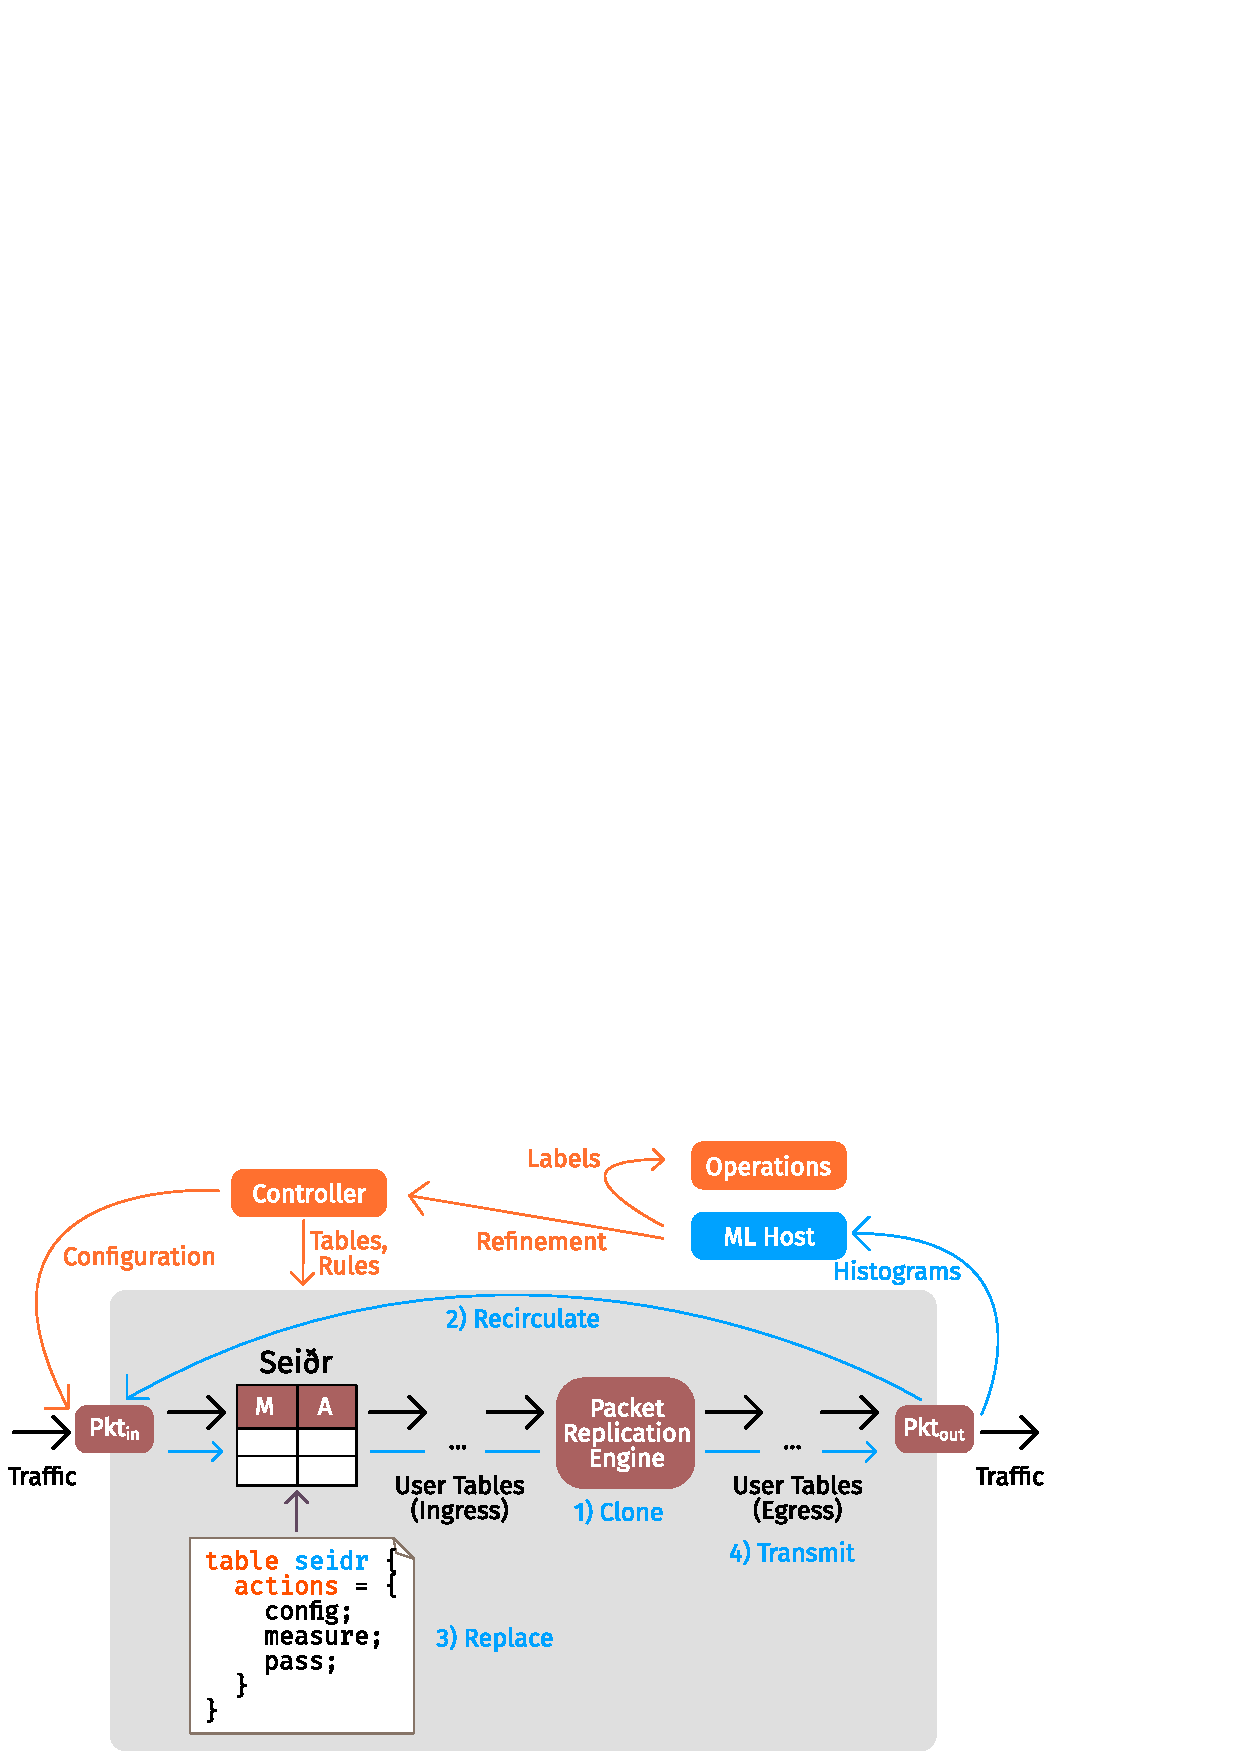
\includegraphics{diagrams/seidr/dp-arch-diagram.pdf}}
    \caption{\seidr{}'s integration with a PSA-compatible~\cite{p4-psa} dataplane.}
    \label{fig:arch}
\end{figure}

% Let's show them a histogram datastructure would look like purely with registers and how would a P4 action populate it - pseudocode or P4 snippet would be nice.

Although packet timing information is useful in understanding network and flow behaviour, without volume or packet rate reduction it is prohibitively expensive for hosts to handle each packet.
Histogramming acts as the \emph{aggregation step} which makes this class of analysis feasible in high-speed networks.
\Cref{fig:arch} demonstrates how \seidr{}, installed as an additional table in any P4 program, records and transmits inter-arrival time histograms.
The format for these histogram packets is outlined in \cref{fig:seidr-headers}; we choose to store individual buckets as \mintinline{rust}{u16}s, and the number of buckets in any histogram is fixed at compile time.
We set this to \num{100} buckets per histogram.
Packets traverse a table which requires \num{3} actions to be implemented:
\begin{enumerate}
    \item \mintinline{rust}{config} reads any matched packets as a \mintinline{rust}{seidr_cfg_t} of type \mintinline{rust}{SET_}\{ \mintinline{rust}{MIN}, \mintinline{rust}{MAX}, \mintinline{rust}{DST}, \mintinline{rust}{SRC}, \mintinline{rust}{LEN} \} by using the P4 parser.
    These update registers \numrange{1}{5} in \cref{tab:registers}, dropping any matched packets.
    
    \item \mintinline{rust}{measure} calculates the inter-arrival time, update per-flow histograms, and transmits finished histograms to the correct host. We describe its operation in \cref{alg:measure}.
    
    \item \mintinline{rust}{pass} ignores packets, and is the default action.
\end{enumerate}
Constructing \seidr{} in this manner allows the control plane to install rules to enable/disable runtime reconfiguration as needed, and to monitor as many or as few flows as desired (\ie, using wildcard rules, or exact matching).

The PSA does not have any mechanisms for generating new packets.
To circumvent this, any packet which would complete a histogram is tagged for cloning at the end of the ingress pipeline, and recirculation at egress (\cref{algline:recirc}).
This truncated copy returns to \seidr{}'s table, where we enable the relevant headers, change L2/3 fields, and write out the histogram contents (\crefrange{algline:rewrite-start}{algline:rewrite-end}).
The P4 deparser outputs the new protocol stack at egress, and transmits the histogram UDP packet into the network.
Event-driven architecture proposals~\cite{DBLP:conf/hotnets/IbanezABM19} may allow a more natural means of packet generation.

\begin{figure}
\centering
\begin{subfigure}{0.45\linewidth}
\centering
\adjustbox{max width = 0.6\linewidth}{
\begin{minipage}{\linewidth}
\begin{minted}[escapeinside=||]{rust}
|\textbf{\textcolor{Keyword}{header}}| seidr_cfg_t {
    bit<8> function;
    bit<144> payload;
}
\end{minted}
\end{minipage}
}
\end{subfigure}
\begin{subfigure}{0.45\linewidth}
\centering
\adjustbox{max width = 0.6\linewidth}{
\begin{minipage}{\linewidth}
\begin{minted}[escapeinside=||]{rust}
|\textbf{\textcolor{Keyword}{header}}| seidr_t {
    bit<128> src_ip;
    bit<128> dst_ip;
    bit<16> src_port;
    bit<16> dst_port;
    bit<16> eth_type;
    bit<BUCKETS * 16> histo;
}
\end{minted}
\end{minipage}
}
\end{subfigure}
\caption{P4 headers for \seidr{} configuration and histograms.}\label{fig:seidr-headers}
\end{figure}

\begin{algorithm}
% \vspace{-0.25cm}
% \DontPrintSemicolon
\KwData{5-tuple, P4 metadata, P4 headers, Registers}
h $\leftarrow$ hash(5-tuple)\;
index $\leftarrow$ BUCKETS * h\;
owner $\leftarrow$ HistoOwner[h]\;
\uIf{metadata.packet\_path = RECIRCULATE}{
    headers.tcp.valid $\leftarrow$ false\label{algline:rewrite-start}\;
    headers.udp.valid $\leftarrow$ true\;
    headers.seidr.valid $\leftarrow$ true\;
    copy 5-tuple into headers.seidr\;
    rewrite headers.ip, headers.udp using HistoSrc/Dest\;
    headers.seidr.histo $\leftarrow$ HistoData[index..]\;
    truncate payload\;
    zero out registers: BucketCount, HistoOwner[h], HistoData[index..]\;\label{algline:rewrite-end}
}
\ElseIf{owner = 0 \textbf{or} owner = 5-tuple}{\label{algline:owner-check}
    HistoOwner[h] $\leftarrow$ 5-tuple\;
    iat $\leftarrow$ LastTimestamp - metadata.mac\_ingress\_time\;
    \If{iat $\ge$ Min \textbf{and} iat $\le$ Max}{
        bucket $\leftarrow$ BUCKETS * (iat - Min) / (Max - Min)\;
        HistoData[index + bucket] $\leftarrow$ HistoData[index + bucket] + 1\;
        BucketCount[h] $\leftarrow$ BucketCount[h] + 1\;
        \If{BucketCount[h] = Len}{
            mark packet for cloning and recirculation\label{algline:recirc}\;
        }
    }
}

\caption{Histogram update and transmission.}\label{alg:measure}
\end{algorithm}

In the event of hash collision (\cref{algline:owner-check}), we ignore packets outside of the tracked flow to ensure that data is accurate.
As later processing and classification directly affect what decisions are made by operators or automatically taken by a policy (possibly leading to incorrect flow limits, QoS, \emph{etc.}), avoiding corruption/cross-contamination of operational data is paramount.
To gain collision resistance, Robin Hood hashing could be used up to a maximum distance in the table, treating a zeroed owner as empty and an illegal source IP as a tombstone value.

\begin{table}
    \centering
    \caption{Register map (Datatype, Amount) for an $h$-bit hash.}
    \resizebox{\linewidth}{!}{\begin{tabular}{@{}ccccccccc@{}}\toprule
        Min & Max & Length & HistoSrc & HistoDest & BucketCount & LastTimestamp & HistoOwner & HistoData \\ \midrule
        \mintinline{rust}{u16} & \mintinline{rust}{u16} & \mintinline{rust}{u16} & \mintinline{rust}{u16 + u128} & \mintinline{rust}{u16 + u128} & \mintinline{rust}{u16} & \mintinline{rust}{u64} & \mintinline{rust}{3 * u16 + 2 * u128} & \mintinline{rust}{BUCKETS * u16} \\
        1 & 1 & 1 & 1 & 1 & $2^h$ & $2^h$ & $2^h$ & $2^h$ \\ \bottomrule
    \end{tabular}}
    \label{tab:registers}
\end{table}

% Basic Logic:
% \begin{itemize}
%     \item table 1: three actions
%     \begin{itemize}
%         \item config: set R1 or R2 (controller installs rule matching a specific port/ip combo)
%         \item measure: take ingress timestamp from metadata, do stuff, write into lasttime, add to bucket and total if within bounds
%         \item pass (default)
%     \end{itemize}
%     \item then pass onto rest of tables
%     \item Why do it this way? can make it all or nothing through control plane.
%     \item How to write and send packet? Same trick as ESNET? (recirc w/ custom metadata to transform pkt)
% \end{itemize}

% ?? NOTE: See PSA \cite{p4-psa} for register format. Some papers, like Dapper, suggest that hash tables should be possible? That would work out very well in our benefit.

% ?? What is configurable? Min, max of the histogramming range

This design allows runtime configuration of all aspects save for the bucket count; at runtime, the only way to increase bucket resolution is to examine a smaller region of IATs.
While in theory this could be configured below a maximum compiled into the firmware, the difficulties introduced in classification/data processing make this infeasible.
Unless using stream-capable classifiers such as LSTMs~\cite{DBLP:journals/neco/HochreiterS97}, changing the input size requires retraining from scratch since new neuron weights must be added and structural properties of the input data change.
Increasing the bucket count requires new firmware installation, as many dataplane P4 implementations cannot allocate variable-length stores due to the lack of a dynamic allocator.

\begin{figure}[t]
    \centering
    \begin{subfigure}[t]{0.49\linewidth}
        \centering
        \resizebox{\linewidth}{!}{\includegraphics{plots/seidr/dt-cubic-1000-app.pdf}}
        \subcaption{TCP Cubic}
        \label{fig:cubic-hist-app}
    \end{subfigure}
    \begin{subfigure}[t]{0.49\linewidth}
        \centering
        \resizebox{\linewidth}{!}{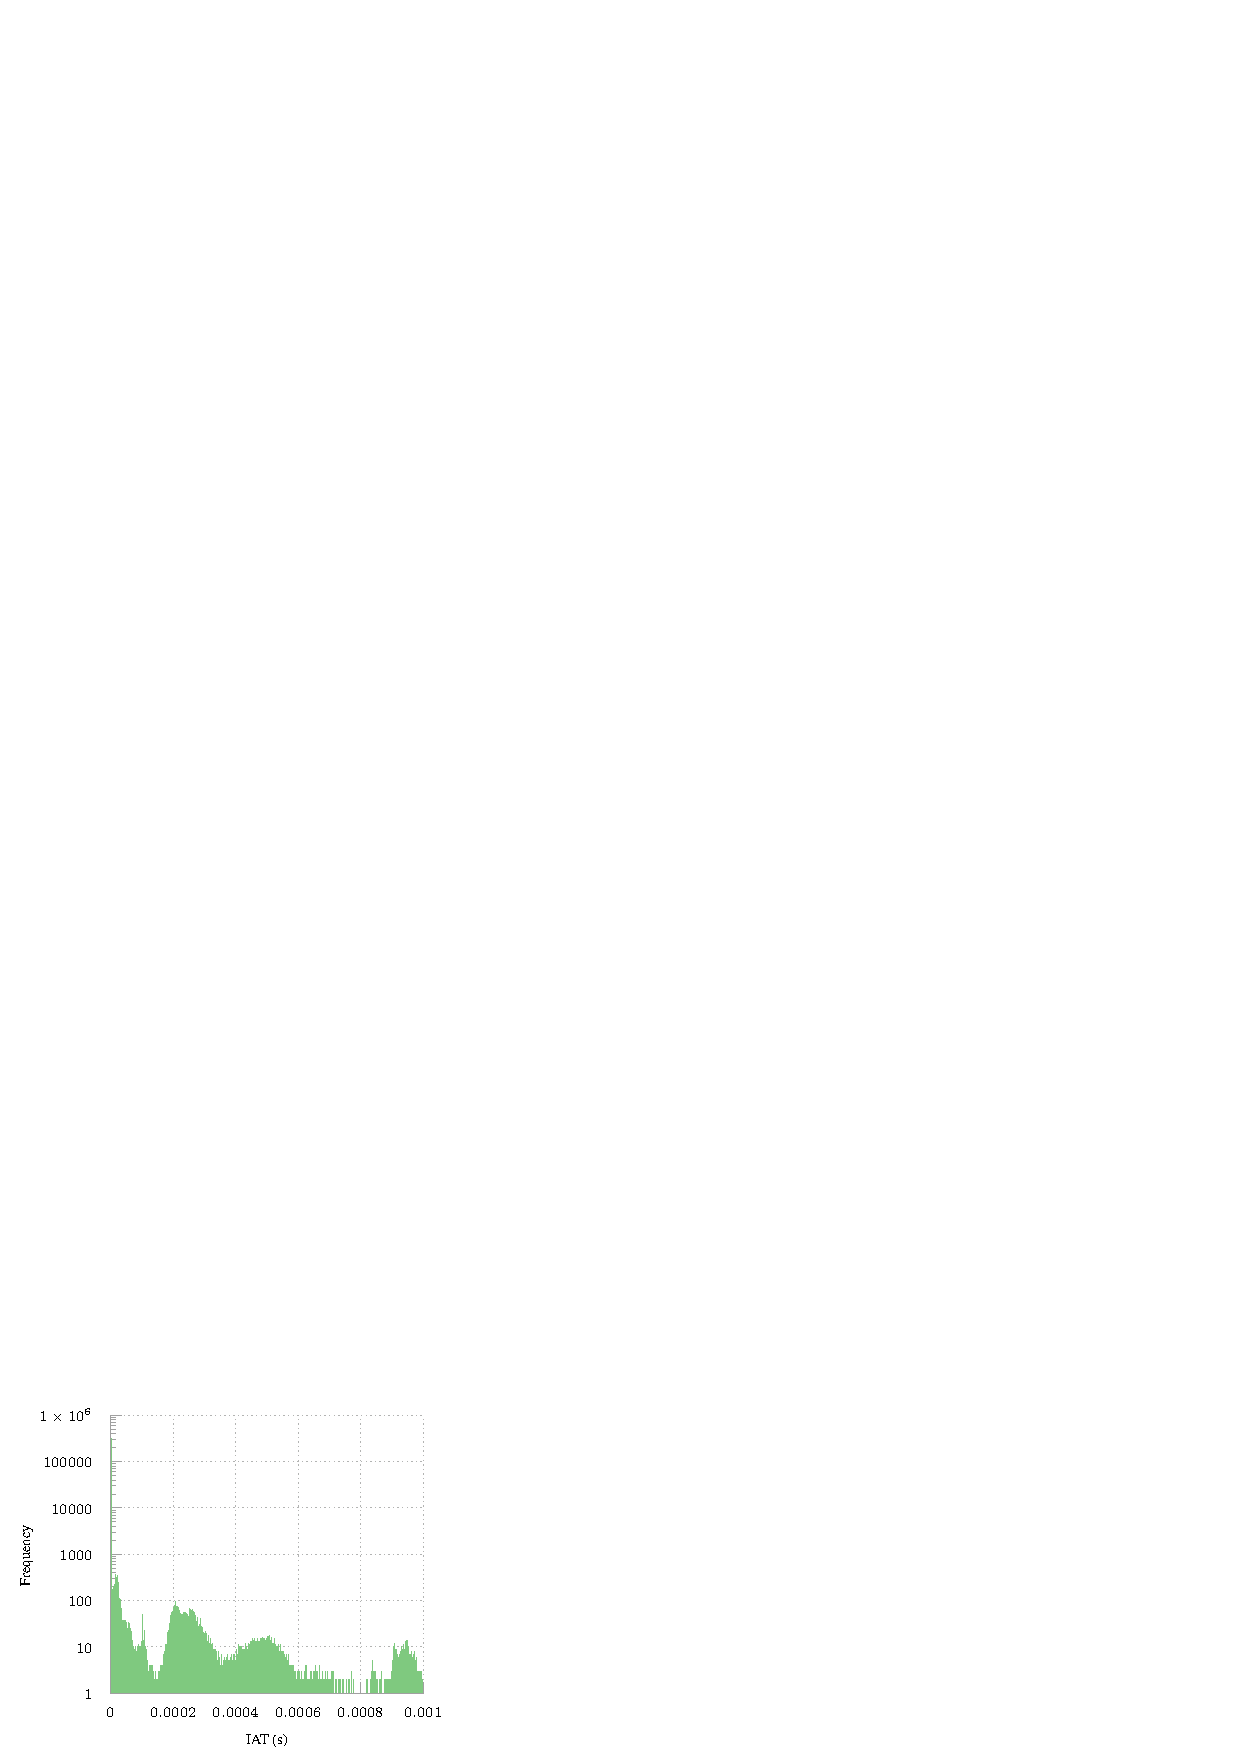
\includegraphics{plots/seidr/dt-bbr-1000-app.pdf}}
        \subcaption{TCP BBR}
        \label{fig:bbr-hist-app}
    \end{subfigure}
    \caption{Example dataplane histograms showing visible differences in inter-arrival times of selected TCP flavours. Our ML solutions are trained to programmatically identify such differences.}
    \label{fig:tcp-hist-app}
\end{figure}

As an example of dataplane-generated histograms, \cref{fig:tcp-hist-app} shows the distribution of inter-arrival times between two TCP congestion control algorithms. The visible differences are programmatically identified using our ML algorithms.

\subsection{Accurate, Precise and High-Resolution Timestamping}

Precise timestamps are critical when detecting temporal properties of flow behaviour, such as microbursts or inferring flow congestion control algorithms.
It is especially important in high speed (\SI{100}{\giga\bit\per\second}) networks, where there can be as little as \SI{6.7}{\nano\second} between packets that need to be analysed.
With a Linux-based software solution (\eg, reading packets from a link with \emph{tcpdump}), the Linux kernel can only provide microsecond-level accuracy with precision in the order of \SI{100}{\micro\second}~\cite{kundel2020p4sta}.
DPDK improves on this, increasing the accuracy to \SI{100}{\nano\second} in the best case~\cite{primorac2017measure}.
However, today's dataplane devices (\eg, Netronome SmartNICs, NetFPGA SUME) allow nanosecond-accurate timestamps to be retrieved from the \emph{Media Access Control} (MAC) modules with a precision of \SI{10}{\nano\second}~\cite{kundel2020p4sta}, a timestamp property \seidr{} relies upon.

% Some platforms provide picosecond-level precision and many solutions allow time synchronisation between multiple devices using the IEEE 1588-2002 (Precision Time Protocol) standard.



\section{TCP congestion control classification}\label{sec:seidr-tcpcc}


% We present an example of first-stage analysis performed for each flow and each packet---stateful TCP analysis.
% This includes numerous metrics which are considered standard when measured at connection endpoints, yet are difficult or invite numerous issues when performed in the network (of which we include a discussion on drawbacks and, curiously, benefits).
% The introduction of accurate timestamps allows us to explore rate-monitoring at a per-packet level, a new view of flow behaviour which may enable flow and hardware characterisation.

% \subsection{Per-Packet Rate Monitoring}

% \begin{figure*}
%     \centering
%     \begin{subfigure}[t]{0.49\linewidth}
%         \centering
%         \resizebox{0.5\linewidth}{!}{
% 	    \begin{tikzpicture}
%     		[packet/.style={draw, fill=uofgsunshine}]
% 		    \node[packet] (p1) {$p_1$: 1500B};
% 		    \node[packet, right= 1cm of p1] (p2) {$p_2$: 800B};
		
% 		    \node at ($(p1.south west) - (0,1)$) (t1) {$t_1$};
% 		    \node at ($(p2.south west) - (0,1)$) (t2) {$t_2$};
		
% 		    \draw[-, dotted] (t1.north)--(p1.south west);
% 		    \draw[-, dotted] (t2.north)--(p2.south west);
		
%     		\draw[<->] (t1.north) -- node[below]{$\mathit{dt}$} (t2.north);
% 	    	\draw[<->] ($(t1.north) + (0,0.2)$) -- node[above]{$s$} ($(t1.north) + (1.8,0.2)$);
% 		    \draw[<->] ($(t1.north) + (1.8,0.2)$) -- node[above]{$g$} ($(t2.north) + (0,0.2)$);
% 	    \end{tikzpicture} 
% 	}
%     \caption{\centering Per-packet rate, visualised. Note that $p_1$ and $p_2$ are not necessarily packets from the same flow.}
%     \label{fig:per-packet-rate}
%     \end{subfigure}
%     \begin{subfigure}[t]{0.49\linewidth}
%     \centering
%     \resizebox{0.9\linewidth}{!}{
% 		\begin{tikzpicture}
% 		[packet/.style={draw, fill=uofgsunshine}]
% 		\node[packet] (p1) {$p_1$: 1500B};
% 		\node[packet, right= 1cm of p1] (p2) {$p_2$: 800B};
% 		\node[right= 1cm of p2] (p3) {...};
% 		\node[packet, right= 1cm of p3] (p4) {$p_{n-1}$: 1500B};
% 		\node[packet, right= 1cm of p4] (p5) {$p_n$: 1500B};
		
% 		\node at ($(p1.south west) - (0,1)$) (t1) {$t_1$};
% 		\node at ($(p2.south west) - (0,1)$) (t2) {$t_2$};
% 		\node at ($(p4.south west) - (0,1)$) (t4) {$t_{n-1}$};
% 		\node at ($(p5.south west) - (0,1)$) (t5) {$t_{n}$};
		
% 		\draw[-, dotted] (t1.north)--(p1.south west);
% 		\draw[-, dotted] (t2.north)--(p2.south west);
% 		\draw[-, dotted] (t4.north)--(p4.south west);
% 		\draw[-, dotted] (t5.north)--(p5.south west);

%         \draw[<->] ($(t2.south) + (0,-0.25)$) -- node[above]{$s$} ($(t2.south) + (6.25,-0.25)$);
%         \draw[<->] ($(t2.south) + (6.25,-0.25)$) -- node[above]{$g$} ($(t5.south) + (0,-0.25)$);
% 		\draw[-, thick] ($(t2.south) - (0,0.5)$) -- node[below]{$W$} ($(t5.south) - (0,0.5)$);
% 		\end{tikzpicture} 
% 	}
%     \caption{\centering Sliding window rate, visualised. Rate estimates are computed using the sizes of the last $W$ packets seen in the current flow. Packets $p_2$ and $p_{n-1}$ belong to the same flow, but $p_n$ is not assumed to.}
%     \label{fig:sliding-window-rate}
%     \end{subfigure}
%     \caption{Comparison of per-packet and sliding window rates. The lengths of packets and inter-packet gaps are not to scale, and are purely demonstrative.}
%     \label{fig:pr-vs-slide}
% \end{figure*}

% Associating each packet with a high-resolution timestamp allows us to introduce the notion of a \emph{per-packet rate}.
% Assuming a packet with size $p$ arrives at time $t_1$ and is followed by another packet (potentially from another flow) which arrives at $t_2$, we measure $\mathit{dt}=t_2-t_1$ for this packet.
% Supposing this first packet spends time $s$ on the wire and assuming that the inter-packet gap $g$ is negligible compared to the length of a packet, then $\mathit{s} = \mathit{dt} - g \approx \mathit{dt}$.
% This packet then has a point rate, $r$:
% \begin{equation}
%     r = \frac{p}{s} \approx \frac{p}{\mathit{dt}}
% \end{equation}
% \Cref{fig:pr-vs-slide} demonstrates how this timing information arises, contrasted with sliding-window rate measurements taken over a longer time period.
% This assumes almost back-to-back traffic, which is realistic in our deployment environment, but to the best of our knowledge no programmable switches expose the timestamp at which the final bit of a packet has been ingested.
% Such a timestamp would allow exact measurement of $s$.

% % ?? we need to be clear about the unintuitive nature of these measurements, include a quick sketch proof which shows that the weighted average of a set of point rates is analytically identical to the sliding window rate/throughput taken over the same period of time.
% While this is an interesting measure to associate with each packet, considering how best to view such rates in aggregate can be counter-intuitive.
% Viewing these rates as time series data reveals interesting distributional characteristics which disagree starkly with our understanding of a flow's rate---for instance, clusters which suggest a different mean.
% Suppose we have a set of measurement indices $C$ with no gaps captured between $t$ and $t'$, partitioned into flows $C = F_1 \cup \dots \cup F_p$.
% To correctly combine a set of point measurements for a flow $F_i$ into an average rate $\overline{r}_{F_i}$, we compute:
% \begin{equation}
%     \overline{r}_{F_i} = \frac{\sum_{a \in F_i} \mathit{dt}_a r_a}{\sum_{c \in C} \mathit{dt}_c}.
% \end{equation}
% In the instance that only one flow is captured (\emph{i.e.}, $F_i = C$), this is a weighted average over point rates, using the $\mathit{dt}$ measured between each packet and the next packet in the same flow as its weight.
% Similarly, this is analytically equivalent to the sliding-window rate measured over the same set of packets:
% \begin{equation}
%     \frac{\sum_{a \in F_i} \mathit{dt}_a r_a}{\sum_{a \in F_i} \mathit{dt}_a} \simeq \frac{\sum_{a \in F_i} p_a}{t' - t}.
% \end{equation}
% % \begin{proof}
% % Given a set of contiguous measurements from the same flow $S \subseteq \mathbb{Z}$, admitting $p_s$, $r_s$, $\mathit{IAT}_s$ and $t_s$, the weighted average of point rates is then
% % $$
% % \overline{r}_S = \frac{\sum_{s \in S} \mathit{IAT}_s r_s}{\sum_{s \in S} \mathit{IAT}_s}
% % $$
% % The sliding-window average:
% % $$
% % \overline{r}_S = \frac{\sum_{s \in S} \mathit{IAT}_s r_s}{\sum_{s \in S} \mathit{IAT}_s}
% % $$
% % \end{proof}

% We assume that inter-packet gaps will be negligible (\emph{i.e.}, that the link is never in a state of very low utilisation), due to typically high utilisation on a WAN.
% % Similarly, we need to discuss the effects of selective monitoring or an abundance of UDP/ICMP traffic (which will distort $dt$s).
% However, this assumption can be distorted if selective TCP flow monitoring is used, or if UDP/ICMP traffic is overabundant; both these scenarios create larger gaps between TCP packets of interest, inflating $g$ to the point where it is comparable in size to $s$.
% This has an impact on our notion of per-packet rates, but not inter-arrival times or other such dependent metrics.
% The effect is small on sliding window rates, particularly at larger window sizes.
% ?? Justify. On paper, it looked like error term was O(1/n), O(g) for an n packet window.


% \section{Inter-Arrival Time}

% Having assigned each packet in a flow with a nanosecond-accurate timestamp ?? tbc

\Cref{fig:tcp-hist-app} suggests that a notable use-case for this type of measurement is \emph{congestion control algorithm} (CCA) detection.
In a TCP connection, each machine is free to choose the CCA it uses to send bytes, and thus how it responds to network congestion signals.
This choice is local, and so is invisible to the other machine (and the network).
In datacentre networks, operators choose these to ensure optimal behaviour.
In a transit network or large WAN however, these hosts (and thus the CCAs in use) are outside the control of network operators, which introduces difficulties when CCA interactions lead to \emph{unfairness}.
Consider the recent (and widespread) introduction of \emph{TCP BBR}~\parencite{DBLP:journals/queue/CardwellCGYJ16}.
\emph{BBR} is a delay/model-based CCA which converges on a fair share of bottleneck bandwidth by reducing its rate if the round-trip time increases, while periodically attempting to increase send rate to account for path/load changes.
However, \emph{BBR} traffic can consume \SI{40}{\percent} of link capacity when multiplexed with loss-based CCAs, regardless of the number of competing flows~\parencite{DBLP:conf/imc/WareMSS19}. 
When ensuring fair transit to all flows, this is hardly a desirable outcome; in fact, it's one which may frustrate clients or violate SLAs.

A curious property of \emph{BBR}'s algorithm which sets it apart from other variants is that packet transmission is \emph{timer-based}.
\texttt{send(packet)}, as defined in the canonical algorithm, asks that on transmission of a packet, the sender should wait for the estimated time that packet would take to reach the recipient.
For instance, at an estimated bottleneck bandwidth of \SI{8}{\mega\bit\per\second}, a \SI{1024}{\kilo\byte} packet would hold back the next packet in the flow until \SI{976.6}{\micro\second} had elapsed.
When packet sizes remain similar this causes strongly periodic behaviour, while mode switches in the \emph{BBR} algorithm cause these periodic bands to shift up or down accordingly.
This effect is stronger than in existing loss- and delay-based algorithms which remain intrinsically tied to the notion of a congestion window (where release of buffered packets follows the receipt of ACK messages).
As a result, timing behaviour of past CCAs may be influenced by (the lack of) packet pacing, periodic components might be made noisier by jitter along the return path, or the behaviour of the receiver might add further noise.

This high-level analysis of \emph{BBR} gives us a strong feature to use as the basis for classification: the \emph{inter-arrival times} (IATs) for each packet in a flow.
We have two options for processing this for classification: we may use a compressed, fixed-size representation such as histograms to capture the aggregate distribution, or we may attempt to capture structural behaviour by using a variable-length stream of IATs.
In many networks, the data and packet rate reduction offered by the former is required to make this possible.
Indeed, in-switch aggregation has seen great success in aiding ML for training~\parencite{DBLP:conf/isca/LiLYCSH19}, and direct execution~\parencite{DBLP:conf/hotnets/XiongZ19}.
We make use of the following standard classification algorithms on a fixed-size representation to attempt to single out the CCA in use:

\begin{itemize}
    \item \emph{$k$-Nearest Neighbours ($k$-NN)}. A simple and well-understood classifier which assigns labels based on the closest members of the training corpus (\ie, by the $L_2$ metric). Linear memory cost in amount of training data, and no training cost other than loading all data points, but capable of learning complex decision boundaries on fixed-length input.
    
    \item \emph{Convolutional Neural Networks (CNNs)}. A neural network approach which learns convolution kernels to classify fixed-length data, particularly when recognising spatial features. Memory cost is fixed for a given architecture irrespective of training data, with a high training cost.
\end{itemize}
% \fakepara{Long Short-Term Memory~\parencite{DBLP:journals/neco/HochreiterS97} units (LSTMs)} A class of recurrent neural network used for stream classification, forecasting, and prediction of variable-length data. Memory cost is fixed, with longer training times (and more data required) than similarly sized CNNs.
% Of these, we apply $k$-NN and CNNs to histograms of packet IATs, and LSTMS to raw IAT streams.

When examining $k$-NN classifiers, we measured accuracy across choices of $k \in \left[2, 8\right]$.
We found $k=2$ to be the most effective choice with our input data using the $L_2$ metric.
Our CNN architecture is described in \cref{tab:cnn-arch}, using ReLu activation and $1 \times 1$ stride in convolutional layers unless stated otherwise.
Training occurred over 5 epochs using the Adam optimiser with categorical cross-entropy as a loss metric, and a batch size of \num{64} histograms (\num{8} for full sequences due to the smaller data volume).
For \emph{BBR vs.\ Cubic}, the complete model consists of \num{104898} 32-bit floating-point parameters (\SI{409.76}{\kibi\byte}), while the full classification task adds a further \num{130} parameters (\SI{0.51}{\kibi\byte}).

\begin{table}
    \centering
    \caption{CNN architecture for \num{100}-entry histograms.}
    \resizebox{0.7\linewidth}{!}{\begin{tabular}{@{}cccc@{}}\toprule
        Layer & Nodes/Filters & Filter Size & Output Dimension \\ \midrule
        Conv2D & 32 & $(3 \times 1)$ & $(98 \times 1 \times 32)$ \\
        MaxPool & --- & $(2 \times 1)$ & $(49 \times 1 \times 32)$ \\
        Conv2D & 64 & $(3 \times 1)$ & $(47 \times 1 \times 64)$ \\
        MaxPool & --- & $(2 \times 1)$ & $(23 \times 1 \times 64)$ \\
        Conv2D & 64 & $(3 \times 1)$ & $(21 \times 1 \times 64)$ \\
        Flatten & --- & --- & \num{1344} \\
        Dense & 64 & --- & \num{64} \\
        Dense (Softmax) & $n_\mathit{classes}$ & --- & $n_\mathit{classes}$ \\
        \bottomrule
    \end{tabular}}
    \label{tab:cnn-arch}
\end{table}


\section{Evaluation}\label{sec:seidr-evaluation}
%Traffic is played back from hosts via Tcpreplay at a bandwidth assigned uniformly from a `good' or `bad' distribution, each using the same pcap file with source and destination IP addresses rewritten.

This work is most naturally compared against Marl, introduced by \textcite{DBLP:journals/eaai/MalialisK15}, the state-of-the-art in \gls{acr:rl}-based \gls{acr:ddos} prevention.
We are most interested in seeing how their approach contrasts with the new agent designs across different topologies and workloads.
Different network environments will also impose different levels of host density, where popular web servers may have orders of magnitude more clients than egress points from their network---I aim to show how these characteristics affect performance and learning rate.
Marl is known to outperform the AIMD~\parencite{DBLP:journals/ton/YauLLY05} strategy, yet the state of the art has long since moved on.
To paint a more current picture, I compare this work against an effective modern approach, \emph{SPIFFY}~\parencite{DBLP:conf/ndss/KangGS16}.
SPIFFY tests a proportion of flows by routing them through an alternate path with higher bandwidth, observing how their speed changes some time later.
This comparison lets us position our new agent designs against the state of the art, observing that SPIFFY has a similar mode of interaction to \gls{acr:rl}-based systems (taking action, observing an effect, and acting once again) and does not rely on protocol characteristics or signatures.
In reimplementing SPIFFY, I make the simplifying assumption that a suitable unused path exists (with identical bandwidth to the server's link).
\qty{10}{\percent} of active flows were tested at a time (according to the authors' observation that there is a factor of \qty{10}{\times} difference between the ideal and achieved bandwidth expansion), excluding flows below \qty{50}{\kilo\bit\per\second} and requiring a \qty{3}{\times} expansion from legitimate flows, making a judgement after \qty{5}{\second}.

To test this, I made use of both traffic models introduced in \cref{sec:a-new-normal} (Opus and \gls{acr:tcp}), both topologies discussed below (1-dest vs.\ Fat-Tree), and vary the amount of hosts typically communicating over each agent's ingress/egress node.
Additionally, these new models were evaluated in multi-agent mode (\emph{separate}, no model sharing), and in single-agent mode (\emph{single}, zero-cost perfect information sharing).
In each case, the algorithm's performance was averaged over \num{10} episodes of length \num{10000} timesteps (setting each agent's $\wvec{}=\mathbf{0}$ between episodes).
Host allocations at the beginning of each episode were generated pseudorandomly to ensure fairness between episodes---a host is malicious with probability $\operatorname{P}\left(\mathit{malicious}\right)$, and is benign otherwise.
Benign hosts generate traffic according to either \cref{sec:tcp-http-traffic-model,sec:udp-opus-traffic-model} depending on the experiment, while malicious hosts generate traffic as described in \cref{sec:attack-traffic-model} (both at experiment-dependent rates).

All experiments were executed on Ubuntu 18.04.2 LTS (GNU/Linux 4.4.3-040403-generic x86\_64), using an Intel Core i7-6700K (\qtyproduct[product-units=single]{4 x 4.2}{\giga\hertz}) which had \SI{32}{\gibi\byte} of \gls{acr:ram}.
%All code underpinning these findings is available on a public repository\footnote{\url{https://github.com/FelixMcFelix/rln-dc-ddos-paper}}.
%All code underpinning these findings is available on a public repository.\footnote{Private until publication.}

\subsection{Single destination}\label{sec:single-dest}
%?? Move description of tree topol to here.
The network is tree-structured, where one server $s$ connects through a dedicated switch to $k$ team leader switches, each connected to $\ell$ intermediate switches, which in turn each connect to $m$ egress switches.
We then have $N_{\mathit{hosts}} = k \ell m n$.
\Cref{fig:marl-topol} demonstrates this.
%Although \citeauthor{DBLP:journals/ccr/MahajanBFIPS02a}, the originators of this topology, make it clear that it exists as a fairly unrepresentative example \cite{DBLP:journals/ccr/MahajanBFIPS02a}, it remains the case that such a network topology allows for functional testing, and indeed is illustrative of one way in which attack traffic might aggregate in the network.
%It is hard, however, to argue its relevance to specific classes of victim or to reason about the interactions it might have with dependent applications.
%We aim to address this through \cref{sec:performance-in-an-emulated-environment}.
The network topology was configured using $k=2$ teams, $\ell=3$ intermediate nodes per team, $m=2$ agents per intermediate node, and $n \in \{2, 4, 8, 16\}$ hosts per learner.
This is a slight simplification of \Textcite{DBLP:journals/eaai/MalialisK15}'s \textquote{online} experiment, choosing fewer teams but remaining as a single server with a fan-out network.
%The algorithm parameters were set at $\gamma=0$ (leading to opportunistic behaviour), $\alpha=0.05$, having linearly annealed $\epsilon=0.2 \rightarrow 0$ by $t=3000$.
%Benign and malicious hosts uploaded between \SIrange{0}{1}{\mega\bit\per\second} and \SIrange{2.5}{6}{\mega\bit\per\second} respectively, and hosts were redrawn at each episode's start with $\operatorname{P}(\mathit{malicious})=0.4$.
%$U_s$  $k \ell mn+2$ \si{\mega\bit\per\second}.
%The performance of each choice of $n$ was averaged over \num{10} episodes of length \num{10000} timesteps (setting each agent's $\wvec{}=\bm{0}$ between episodes).
%Host allocations were generated pseudorandomly to ensure fairness between choices of $n$.
%These parameter choices match those of the original study to enable direct comparison, and are (to the best of our knowledge) arbitrary, but we justify our range of $n$ as capturing increasing scales of host activity.

\begin{figure}
	\centering
	\resizebox{0.9\linewidth}{!}{\begin{tikzpicture}[
	texts/.style = {text=black},
	labeltexts/.style = {text=uofgsandstone},
	treeline/.style = {draw=uofgburgundy},
	treenode/.style = {texts, circle, centered, fill=white, treeline},
	load/.style = {fill=uofgcobalt},
	loadhide/.style = {fill=uofgcobalt!40!white},
	external/.style = {fill=uofgrust},
	externalhide/.style = {fill=uofgrust!40!white},
	hideline/.style = {draw=uofgsandstone!40!white},
	hidenode/.style = {treenode, hideline},
	grow'=right
]
	\node[treenode, label={[texts]above:Server}] (root) {}
	child [treeline] { node [treenode, label={[texts]above:Core}] (sswitch) {}
		child [treeline] { node [treenode, label={[texts]above:Leader}] (teaml) {} 
			child [treeline] { node [treenode, label={[texts]above:Intermediate}] (inter) {}
				child [treeline] { node [treenode, load, label={[texts]above:Agent/Egress}] (agent) {}
					child [treeline] { node [treenode, external] (extern) {}
						child [treeline] { node [treenode, external, label={[texts]above:Host}] (host) {} }
						child [hideline] { node [hidenode, externalhide] (endhost) {} }
					}
				}
				child [hideline] { node [hidenode, loadhide] (endagent) {} }
			}
			child [hideline] { node [hidenode] (endinter) {} }
		}
		child [hideline] { node [hidenode] (endteaml) {} }
		edge from parent
		node[below, labeltexts] {$U_s$}
	};
	
	%\draw[-] (teaml) -- (endteaml);
	\node [labeltexts] (kdots) at ($(teaml)!0.5!(endteaml)$) {$\rvdots$};
	\node [labeltexts, right = -0.1cm of kdots] {$k$};
	\node [labeltexts] (ldots) at ($(inter)!0.5!(endinter)$) {$\rvdots$};
	\node [labeltexts, right = -0.1cm of ldots] {$\ell$};
	\node [labeltexts] (mdots) at ($(agent)!0.5!(endagent)$) {$\rvdots$};
	\node [labeltexts, right = -0.1cm of mdots] {$m$};
	\node [labeltexts] (ndots) at ($(host)!0.5!(endhost)$) {$\rvdots$};
	\node [labeltexts, right = -0.1cm of ndots] {$n$};
\end{tikzpicture}}
	\caption[Tree-structured network topology diagram for evaluating a single-destination network.]{
		Network topology diagram, showing how the server and its core switch's $k$ teams are structured, with $\ell$ intermediate routers per team, connected to $m$ agents which each moderate $n$ hosts beyond a single external switch.
		%	Empty nodes are considered to be internal.
		Red nodes are external, and each blue node hosts an agent.
		\label{fig:marl-topol}
	}
\end{figure}

\subsection{Multiple destinations}
The previous topology allows for direct comparison against the state-of-the-art, and indeed is illustrative of one way in which attack traffic might aggregate in the network.
It is hard, however, to argue its relevance to specific classes of victim or to reason about the interactions it might have with dependent applications.
In contrast, the fat-tree topology~\parencite{DBLP:conf/sigcomm/Al-FaresLV08} sees regular use in real-world data centres and scales well horizontally.
%?? Come up with description of fat-tree (multi-dest) topol.
%?? Why fat tree? regularly appears in modern datacentres.
%?? $k=4$ fat-tree , with one pod hosting two servers $s_0,s_1$.
We use a $k=4$ fat-tree, with one pod hosting two servers $s_0$ and $s_1$.
$n$ external hosts connect through each core switch (where agents are hosted), and communicate with $s_0, s_1$ uniformly randomly.
Both servers host identical services.
We set $n \in \{6, 12, 24, 48\}$ hosts per learner (keeping $N_{\mathit{hosts}}$ identical to each tier of the single-host topology), and restrict $U_{s_0} = U_{s_1} = U_s / 2$.

\subsection{Parameters}
The algorithm parameters were set at $\alpha=0.05$, linearly annealing $\epsilon=$ \num{0.2} $\rightarrow$ 0 by $t=$~\num{3000} in the case of Marl (\num{8000} actions per agent in the \emph{Instant/Guarded} models).

Benign hosts each occupied \qtyrange{0}{1}{\mega\bit\per\second}, and hosts were redrawn at each episode's start with $\operatorname{P}(\mathit{malicious})=$~\num{0.4}.
%The original introduction of this approach to direct-control reinforcement learning as introduced by \textcite{DBLP:journals/eaai/MalialisK15} fails to consider key cases: the absence of a suitable heuristic classifier $g(\cdot)$, disjoint ranges of traffic distribution (i.e., the presence of benign heavy-hitters), the accurate simulation of TCP-like behaviour (and its effects on collateral damage), and high densities of hosts at egress points.
%?? Why? ...
%Of these, the latter two are most deserving of a closer investigation, as they have stronger implications for wide-scale deployment.
%These are important issues, particularly when we consider real-world deployment.
%Heuristic estimates of traffic legitimacy come with computational cost and couple the reward function to the accuracy of the estimator, hosts often show diversity in their own traffic patterns (perhaps being multi-modal), and it is known that TCP is the most used transport protocol for Internet traffic \cite{DBLP:conf/saint/ZhangDJC09}.
%?? NEED TO VERIFY VOLUME OF CONGESTION-AWARE PROTOCOLS
Malicious hosts each sent \qtyrange{2.5}{6}{\mega\bit\per\second} when attacking \gls{acr:udp} traffic, though this was increased to \qtyrange{4}{7}{\mega\bit\per\second} when using \gls{acr:tcp}-like traffic (to meaningfully impact benign flows).
Given $n$ and $\operatorname{P}(\mathit{malicious})$, we see an expected malicious bandwidth \numrange{1.27}{1.87} and \qtyrange{2.03}{2.18}{\times} $U_s$ respectively.
%The expected fraction of $U_s$ consumed by each host is \SI{21.5}{\percent} for $n=2$, and \SI{2.84}{\percent} for $n=16$.
For these choices of $n$ in both topologies, we observe $N_{\mathit{hosts}} \in \left\{24, 48, 96, 192\right\}$, and an expected number of malicious hosts $\mathbb{E}\left[N_{\mathit{attackers}}\right] \in \left\{9.6, 19.2, 38.4, 76.8\right\}$.
For the largest choice of $n$, we see an expected total attack traffic $\mathbb{E}\left[V_{\mathit{attack}}\right] =$ \qtylist{334.05;422.4}{\mega\bit\per\second} for Opus and \gls{acr:http} traffic respectively.

$U_s$ was fixed at $N_{\mathit{hosts}}+2$ \unit{\mega\bit\per\second} (to account for burstiness), and each link had a delay of \qty{10}{\milli\second}.
All links had unbounded capacity, save for each server-switch.
These parameters match those of the original study to enable direct comparison, and many are (to the best of our knowledge) arbitrary, but I justify the range of $n$ as capturing increasing scales of host activity.

% \section{Related Work}\label{sec:related}
% %?? Try and compare my work here when possible?

\fakepara{DDoS Prevention}
\Textcite{DBLP:conf/lcn/BragaMP10} examine the detection of flooding DDoS attacks through \emph{self-organising maps}, using SDN to gather statistics effectively.
Many of their features aren't overly relevant, as their focus is not active defence or discovering \emph{which} hosts contribute to an attack.
%?? Actually talk about Marl (???) to appease reviewer \#1.
The closest available approach within this field is that of \textcite{DBLP:journals/eaai/MalialisK15} (whom we have positioned our work against), and their contribution in applying RL to the task of intrusion prevention is significant: their work helps to show the viability of live, adaptive, feedback-loop-like control of the network to detect and prevent DDoS attacks.
They create a tree overlay topology (subdivided into teams), where each agent applies packet drop to \emph{all} flows inbound to a protected server.
%?? Recap their flaws, since they've been cut form every other aspect.
Our results show that their technique underperforms at high host density and when congestion-aware traffic dominates---that their results do not demonstrate this suggests an evaluation driven purely by traces (rather than live application dynamics).

\emph{SPIFFY} \cite{DBLP:conf/ndss/KangGS16} aims to remedy transit-link attacks by observing how flows from each source respond to a sudden increase in available bandwidth.
\Citeauthor{DBLP:conf/ndss/KangGS16} realise that bots participating in an attack are often unable to match this bandwidth expansion (having already saturated the capacity of their outbound links), while legitimate flows typically speed up to match the new fair-share rate.
%Attackers must either be detected or reduce the throughput of each bot, increasing the cost of launching an attack.
%Unlike our approach (and due to the class of attacks it is designed to defend against), SPIFFY is intended to be deployed within ASes, although .
A weakness of their approach is that computing a route to measure bandwidth expansion on real networks can be costly (up to \SI{14}{\second} for the Cogent topology), and that the low expansion factors in real network can require more ``rounds'' of filtering.
By contrast, our approach takes a constant time to compute an action for a flow regardless of topology size.
Their assumptions about traffic response to such bandwidth expansion do not hold for constant bitrate flows (e.g., VoIP) and may not extend to HTTP DASH flows, both of which make up a sizeable proportion of network traffic.

\emph{Athena} \cite{DBLP:conf/dsn/LeeKSPY17} is a generalised SDN framework for intrusion detection, but has shown the use of a \emph{k-nearest neighbours} classifier to detect individual attack flows.
Although heavyweight (and proven to be effective compared with \textcite{DBLP:conf/lcn/BragaMP10}), their comparison against SPIFFY lacks the quantitative evidence required to understand how the system compares.
\Textcite{DBLP:conf/sp/SmithS18} use AS-level routing to tackle both transit-link and flooding-based attacks.
This view is taken due to the perceived cost of per-stream classification and inherent sensitivity to adversarial examples.
The approach is creative, relying upon BGP \emph{fraudulent route reverse poisoning} to preserve traffic to a target AS, but unlike SPIFFY the approach doesn't actually \emph{remove} the congestion.
Because of this, flooding-based attacks aren't fully alleviated.

%?? Abuses of RL 
\fakepara{RL in Networks}
Earnest, well-considered application of RL towards the challenge of intrusion prevention has seen comparatively little examination.
Past work treats the paradigm as a traditional classifier for anomaly detection \cite{shamshirband2014anomaly} and DDoS prevention \cite{DBLP:conf/mates/ServinK08}.
Given that the main strengths of RL techniques are the ability to control ongoing interaction and adapt by observing the concrete effects of actions, such works don't apply the rich literature on the subject to its fullest potential.

For categorising how RL fits into solving problems, we label works as direct- or indirect-control RL.
A \emph{direct-control} RL problem is one where the RL agent(s) learn optimal control over a set of actions as the \emph{primary} defence or decision-maker---requiring measurements, reward functions and action sets tailored for this purpose.
%We feel there is a shortage of work in this category at present, at least in the field of networks.
To date, the best-fitting example we have encountered is that of \textcite{DBLP:journals/eaai/MalialisK15}.
An \emph{indirect-control} RL problem is one where agents act in service to \emph{another technique} responsible for decision-making, optimising or generalising aspects of its operation beyond that of hand-coded heuristics.
A past example includes learning when best to share knowledge between \emph{hidden Markov model} anomaly detectors \cite{DBLP:conf/paisi/XuSH07}.
%The position of this work is weakened by its reliance on the problematic `DARPA99' dataset \cite{DARPA-IDD, DBLP:conf/cisda/TavallaeeBLG09, DBLP:conf/sp/SommerP10}, but the idea itself is well-treated and this acts as a driver for improvements in this direction.
This work is weakened by its reliance on the problematic `DARPA99' dataset \cite{DBLP:conf/sp/SommerP10}, but the idea itself is well-treated.
Outside of intrusion detection, there has been growing interest in the use of RL in data-driven networking, such as for intra-AS route optimisation \cite{DBLP:conf/hotnets/ValadarskySST17} and resource-constrained process allocation \cite{DBLP:conf/hotnets/MaoAMK16}.
\textcite{DBLP:conf/sigcomm/MaoNA17} employ client-side observations of network state and video performance with RL to optimise bitrate selection for multimedia streaming.
\emph{AuTO} \cite{DBLP:conf/sigcomm/ChenL0L18} employs deep RL to perform traffic optimisation.
Crucially, they find that the vast majority of flows are short-lived, requiring effective decisions in less than a millisecond.
To overcome the high latency of action computation via a neural network, two agents are trained, handling aspects of short and long flows respectively.
The first learns to optimise the flow size thresholds to demarcate long and short flows; these short flows are routed by ECMP.
The second agent makes bespoke decisions about routing, prioritisation etc.\ for each of the remaining long flows.


\section{Summary}\label{sec:seidr-conclustion}
We have presented \seidr{}, a dataplane assisted flow classification solution that can be used to detect fine-grained temporal flow behaviour. We have shown a PSA-compliant way to implement in-network data aggregation in the form of histograms, while using nanosecond-precision timestamping. Our in-network generated histogram datastructure (\eg, on per-flow packet inter-arrival times) has been presented as the input for various ML algorithms, including CNN and $k$-NN. We have shown with our extensive evaluation that \seidr{} can successfully tell apart TCP CCAs, in particular, it identifies BBR from its predecessors with over \SIrange{88}{96}{\percent} accuracy, while only consuming a maximum \SI{15.5}{\mebi\byte} of dataplane memory. We presented the trade-offs between training and inference times, memory requirements, and accuracy in the context of CNN and $k$-NN classifiers and shown that \seidr{} outperforms prior work by increasing classification accuracy on novel TCP CCAs, providing the ability to classify at very high traffic rates (in the order of \SI{10}{\tera\bit\per\second}).
Furthermore, we have identified a key temporal property of \emph{BBR} which allows its easy detection among other flows.
In the future, we aim to examine the use of \seidr{} towards microburst detection and diagnosis~\cite{DBLP:conf/sigcomm/ChenFKRR18} and for the identification of \emph{BBR}-like temporal properties of emerging UDP-based congestion-aware protocols, such as \emph{QUIC}.%~\cite{DBLP:conf/sigcomm/LangleyRWVKZYKS17}.

?? Through this chapter, we have discussed ..., lending credence to one of the claims in my thesis statement: \superrecallthesis{3}


% -----

%\part{Background}
\chapter{Scalable Flow Classification}\label{chap:seidr}

% \section{Motivation}
% \section{Sei\dh{}r Histograms}
% \subsection{Algorithm}
% \subsection{Packet Generation on PSA}
% \section{Use case: TCP CCA Detection}
% \subsection{Observable Differences}
% \subsection{Investigating the BBR Algorithm}
% \section{Methodology}
% \subsection{Testing Environments}
% \subsection{Data Collection/Generation}
% \subsection{ML Model Architecture}
% \section{Evaluation}
% \subsection{Device Memory Costs}
% \subsection{Bandwidth Costs}
% \subsection{CCA Detection Accuracy and Costs}

?? Problem statement: damn, all this ML is cool
?? We can do cool real-time analysis of operational Internet traffic
?? What do we do if we need more complex ML models: i.e., need to use LSTMs, or complex CNNs because we need to make use of complex temporal or structural features of data? We still need to get it to host machonies.
?? Okay... but in that case, how can we reduce data so that PPS and Gbps of data don't overwhelm the host, or that we lose lots of asid data and make poor decisions when we have many (or very fast) flows?

?? Relate some of this \emph{specifically} back to discussion of flow measurement in the dataplane in the INC use-cases? (i.e., considering all th below IPfix, sFLow, etc. etc.)
?? Try to relate some of the same problems.

There has been significant research and development on real-time analysis of operational Internet traffic.
Accurate flow characterisation (or \emph{classification}) can drive intrusion detection, detecting unusual or illegal patterns of network traffic, or to prioritize traffic for certain customers, to provide path-diversity as well as to mark Quality of Service (QoS) of various users and protocols~\parencite{DBLP:journals/ccr/BernailleTASS06,DBLP:conf/lisa/Roesch99}.
However, flow classification solutions today can usually only rely on sampled data provided by routers, such as sFlow, Netflow, or IPFIX, along with imprecise timing (\si{\micro\second} and \si{\milli\second}-level)~\parencite{rfc7011,rfc3954}.
While sampled, low-precision telemetry can be used to classify network traffic based on some flow properties (such as port and protocol numbers)~\parencite{DBLP:conf/iwcmc/RossiV10}, it cannot be used to classify based on fine temporal properties (\eg, identifying bursty flows and senders that can cause microbursts and buffer overflow on the network).

On the other hand, full-software solutions for traffic classification have been proposed by commercial vendors (\eg, Barracuda DPI\footnote{https://www.barracuda.com/glossary/deep-packet-inspection}), the open-source community (\eg, Snort~\parencite{DBLP:conf/lisa/Roesch99}, Zeek (formerly Bro)~\parencite{DBLP:conf/uss/Paxson98,zeek}), and the research community, with extensible feature sets and algorithms for classification~\parencite{DBLP:conf/icccn/HagosEYK18}.
Unfortunately, these software solutions designed for commodity hardware do not provide accurate timing of packets, and therefore make certain time-critical events hard or impossible to detect (\eg, microbursts~\parencite{DBLP:conf/sigcomm/ChenFKRR18} or congestion control properties~\parencite{DBLP:conf/icccn/HagosEYK18}).
Moreover, even the most sophisticated software solutions process packets orders of magnitude slower than current backbone traffic of large operators, making them unusable for large-scale operational analysis~\parencite{DBLP:journals/wpc/ParkA17}.

At the same time, programming and fast reconfiguration of network devices is being explored in all types of networks: datacenter and cloud networks, CDNs and WANs.
Specifically, with the recent developments of generalized dataplanes (\eg, the \emph{Portable Switch Architecture}~\parencite{p4-psa}), target devices (\eg, Barefoot Tofino and Netronome SmartNICs) along with the high-level programming languages presented for them (\eg, P4~\parencite{DBLP:journals/ccr/BosshartDGIMRSTVVW14}), operators can now express in-network functionality running on their devices, including accurate nanosecond-precision packet timing.
However, programming in-network services has its own challenges (\eg, restricted instruction sets, data types and memory), prohibiting the implementation of a fully in-network classification solution.

% To solve the aforementioned challenges, this paper presents an architecture that marries the precision timing and fast data aggregation capabilities of the dataplane with software classifiers that can run complex classification models due on a the reduced data rate.

To solve the aforementioned challenges, we present \seidr{}\sidenote{Pronounced ``SAY-ther''. ?? Explain naming?}, a dataplane assisted flow classification solution.
Our design philosophy of \seidr{} keeps functionality where it belongs: dataplane devices create accurately timestamped, aggregated data structures for our analysis, and we let a scalable software stack perform ML-based classification on commodity machines.\sidenote{?? Yeah this directly contradicts the main theme and line of reasoning of my thesis LMAO}
As in-network aggregation reduces the data rate by a factor of $\sim$\num{740}, our solution can analyse aggregated data from a total rate of \SI{10}{\tera\bit\per\second} original traffic using a single commodity processing machine.

As a concrete use-case, we look at fine dynamics of TCP congestion control algorithms.
Understanding and classifying them is important for network providers as inadequate choices have severe effects on transfer rates, especially in networks with high bandwidth-delay product~\parencite{DBLP:journals/queue/CardwellCGYJ16} and in networks where multiple congestion control algorithms are used~\parencite{DBLP:conf/imc/WareMSS19}. 
By using accurate congestion control diagnostics, operators will be able to infer sender problems (\eg, backlogged or application-limited senders), network inefficiencies (\eg, increased path latency and congestion), as well as receiver issues (\eg, delayed acknowledgements, small receiver windows) and fairness issues between delay-based and loss-based algorithms~\parencite{DBLP:conf/imc/WareMSS19}.

The contributions of this paper are summarized below:
\begin{itemize}
	\item A flexible dataplane-assisted architecture compatible with the \emph{Portable Switch Architecture} (PSA)~\parencite{p4-psa} that allows data aggregation in the form of histograms with nanosecond-accurate timing (\Cref{sec:architecture}),
	\item A high-accuracy method for telling apart timer-based (\eg, BBR) and cwnd-based TCP flavours using our system with machine learning algorithms (\Cref{sec:tcpcc}),
	\item An extensive evaluation of TCP congestion control classification using our solution (\Cref{sec:evaluation}).
\end{itemize}

The work presented in this chapter considers how \gls{acr:pdp} hardware can reduce input, though fine-grained, measurements into digests suitable for \gls{acr:ml} models running on host machines, and is based upon \citetitle{DBLP:conf/globecom/SimpsonCP20}~\parencite{DBLP:conf/globecom/SimpsonCP20}.
?? Then summarise contents from here...

?? Big open qs:
?? relevance of PSA digests? These can emit packets, no? These can emit an arbitrary struct to the ctl plane over P4Runtime API. Might be good if no digest support, . Digests have a few extra benefits: In some dataplanes can be emitted in egress. Is message fusion a possible downside? (unpredictable)
?? Maybe 2 options? Can be in-band or out-of-band. Digests are the out-of-band option, meanwhile in-band allows you to use dataplane to forward to accelerators like BrainWave (don't add extra load to ctl plane in this way?)

?? Header size limits are the other main constraint.
?? THis is probably not a problem with digests.
?? WHen emitting to dataplane, however? Will have plat-dependent limits on output. Header size limits, PHV limits, register access reqs that could prevent digest access? Need to mark in-progress histo emissions, progress for each, and emit bitslices spread over multiple egress pkts. Logic: CLONE LOOP WHile still pkts to write, block updates to histo if progress (1 bit?). Limitation: Histo emission freq must be reduced to prevent massive traffic amp. slicing logic could be extended to include the digest case? Are there PHV limits in the digest case that make this really suck?

%\section{Introduction}\label{sec:seidr-introduction}
%Network anomaly detection and intrusion detection/prevention are continually evolving problems, compounded by the partial, non-\emph{independent and identically distributed} (IID) view of data at each point in the network.
Attacks and anomalous behaviours evolve, becoming more sophisticated or employing new vectors to harm a network or system's confidentiality, integrity, and availability without being detected \cite{DBLP:journals/comsur/BhuyanBK14}.
These attacks and anomalies have measurable consequences and symptoms which allow a skilled analyst to infer new signatures for detection by misuse-based classifiers, but unseen attacks may only be defended against after-the-fact.
This issue is inherent to \emph{misuse-} or \emph{signature-based} intrusion detectors, and it has been long-hoped that \emph{anomaly-based} detectors would surpass this by making effective use of statistical measures \cite{DBLP:journals/comsur/BhuyanBK14}.

While \emph{machine learning} (ML) approaches seem like a sensible fit for this problem, in \citeyear{DBLP:conf/sp/SommerP10} \citeauthor{DBLP:conf/sp/SommerP10} identified the `failure to launch' of ML-based anomaly detection systems---a distinct lack of real-world system deployments \cite{DBLP:conf/sp/SommerP10}.
To quite a large extent, this remains the case today.
They posit that their use is made difficult due to significant operational differences from standard ML tasks, including: the high cost of errors and extraordinarily low tolerance for false positives inherent to network intrusion detection \cite{DBLP:conf/ccs/Axelsson99}; a general lack of recent, openly available (and high-quality) training data; and diversity of network traffic across varying timescales combined with significant burstiness \cite{DBLP:journals/ccr/LelandWTW95}.
Above the aggregate level, the constant deployment of new services and protocols means that traffic is \emph{non-stationary} and displays an evolving notion of normality.
Learning is made harder still by the challenges encountered with unlabelled (often partial) data.
All of these factors greatly inflate the difficulty of the detection problem.

%?? Make it clearer here what problem I specifically want to solve: principally a particular class of DDoS attacks; volume-based DDoS attacks. Amplification attacks are just a specialisation, this can be made more obvious. I think I need to be clearer about the \emph{intended deployment environment} of service hosts (i.e., not ISPs).

For certain classes of problem e.g., volumetric \emph{distributed denial of service} (DDoS) attacks, \emph{reinforcement learning} (RL) offers another perspective.
%?? Unclear explanation of RL here?
RL agents operate by following a \emph{policy} to interact with or control a system, while at the same time using observed performance metrics and deliberate exploration to dynamically improve this policy.
In this way the role of a RL agent differs from that of a standard classifier, adaptively reacting to threats by assuming the role of a feedback loop for network optimisation, typically to safeguard service guarantees.
In a sense, this allows us to ``overcome'' some of the difficulties of the detection problem by monitoring \emph{performance characteristics and consequences} in real-time; by looking for (and controlling) the effect rather than the cause.
Long-term, we expect that the value of RL-based defence systems will be to augment what existing misuse-based solutions can provide, by automatically alerting, recording and controlling what are believed to be illegal system states.
The goal of this work is much less general; we aim to prevent volume-based DDoS attacks with the aid of RL-based techniques (an important goal in its own right), while bringing to light the flexibility and applicability of these techniques in the security domain.
%Whether it takes direct control of the network, or is used indirectly to optimise a key part of another system, more powerful `deep' RL techniques (and well-founded action spaces) aren't yet well explored for network IDS/IPS.
%These range from more modern training algorithms \cite{DBLP:journals/corr/SchulmanWDRK17, DBLP:conf/icml/SchulmanLAJM15}, to evolutionary strategies \cite{DBLP:journals/corr/SalimansHCS17, DBLP:journals/corr/abs-1802-08842}, hierarchical action composition \cite{DBLP:journals/corr/abs-1710-09767}, and competitive multi-agent learning \cite{DBLP:journals/corr/abs-1710-03748}.

To date, there have been few applications of this class of algorithms towards intrusion detection and prevention which make use of their full potential for online control, rather than using them as the basis for a classifier.
We aim to take steps to redress this and establish their proper capabilities, beyond simple ``blind application''.
%?? Expand as required
What approaches do exist are aimed towards the task of adaptive online DDoS mitigation, and rely upon learning to control probabilistic packet drop.
%?? THAT IS A MAJOR CONTRIB, MENTION IT EVERYWHERE YOU CAN

%?? Discuss the most important conclusions before the outline.
We find that the existing work for this task \cite{DBLP:journals/eaai/MalialisK15} fails to account for congestion-aware traffic (i.e., TCP) and environments with high host density per egress point, achieving poor results due to an overly coarse view of the network.
To remedy this, we make throttling decisions on a per-source basis and present the engineering decisions this mandates: updating RL agents from multiple traces per timestep, timed random sequential action computation and a supporting \emph{software-defined network} (SDN) architecture.
In tandem with the development and evaluation of an effective state space and model, we provide the design of a second model inspired by past work on algorithmic DDoS prevention, as an example of the integration of domain-specific knowledge.
Our introduction of per-source decisions improves substantially upon the state-of-the-art when acting upon most internet traffic (i.e., congestion-aware protocols), and we show that our second model achieves excellent performance for high host density in this case.
Crucially, both models remain protocol- and content-agnostic to offer future-proofing against the rollout of future protocols like QUIC \cite{DBLP:conf/sigcomm/LangleyRWVKZYKS17}.
%?? Also algorithmic enhancements such as multiple actions per timestep, 
%?? PROTOCOL-AGNOSTIC -- HOW WILL THESE THINGS COPE WITH QUIC ET AL.?!?!

\subsection{Contributions}
This paper contributes two source-level granularity approaches to RL-driven DDoS prevention (\emph{Instant} and \emph{Guarded} action models), improving upon past aggregate-based models (\cref{sec:ddos-mitigation-with-per-flow-reinforcement-learning}).
These are designed to make effective decisions irrespective of protocol, and act on individual flows at the edge of any network topology.
We offer an in-depth investigation into suitable features for automatic DDoS mitigation, with qualitative and quantitative justification (\cref{sec:rethinking-the-state-space}).
These features have been suggested by past studies, and independently tested in their own contexts.
Our study is the first attempt to quantify the individual efficacy of each in an RL setting.

We implement reactive simulations of HTTP and VoIP web-server traffic, designed to test system characteristics that packet trace playback fails to capture (\cref{sec:a-new-normal}).
To our knowledge, this is the first attempt to study or replicate Opus-based VoIP traffic, which has become commonplace since the codec's release in 2012.
These new traffic models inform an empirical evaluation of our new models against the state-of-the-art in RL-based DDoS mitigation using (\cref{sec:the-results-of-doing-so}), alongside a discussion of security concerns and real-world deployment (\cref{sec:discussion}).
We additionally compare our work against SPIFFY \cite{DBLP:conf/ndss/KangGS16}, reuniting two divergent strands of research and grounding the study of RL-based DDoS defences.

\section{Telemetry creation in the dataplane}\label{sec:seidr-architecture}


%  No need for this... space issues
% \begin{figure}
%     \centering
%     \resizebox{0.7\linewidth}{!}{\includegraphics{plots/Hyllus-architecture.pdf}}
%     \caption{Architecture (placeholder).}
%     \label{fig:arch}
% \end{figure}

% As shown on Figure~\ref{fig:arch},



\subsection{Limitations of Programmable Dataplanes}
While dataplane programming promises easy reconfiguration of network devices, it poses some challenges.
First, network devices support only a limited set of operations and control flows (no loops) without use of platform-specific \mintinline{rust}{extern}s, and restrict the user to specific primitive data types, \ie, no floating-point units due to tight hardware constraints.
Second, these devices have limited low-latency memory (on the order of a few tens of \si{\mega\byte}s~\cite{jin2017netcache}) and do not provide dynamic memory management.
These limitations prohibit complex algorithms from being implemented, but allow certain restricted solutions, such as what is presented in DAPPER~\cite{DBLP:conf/sosr/GhasemiBR17}, where the authors implement a TCP state machine purely in the dataplane.

\subsection{Histogram Generation}

\begin{figure}
    \centering
    \resizebox{0.8\linewidth}{!}{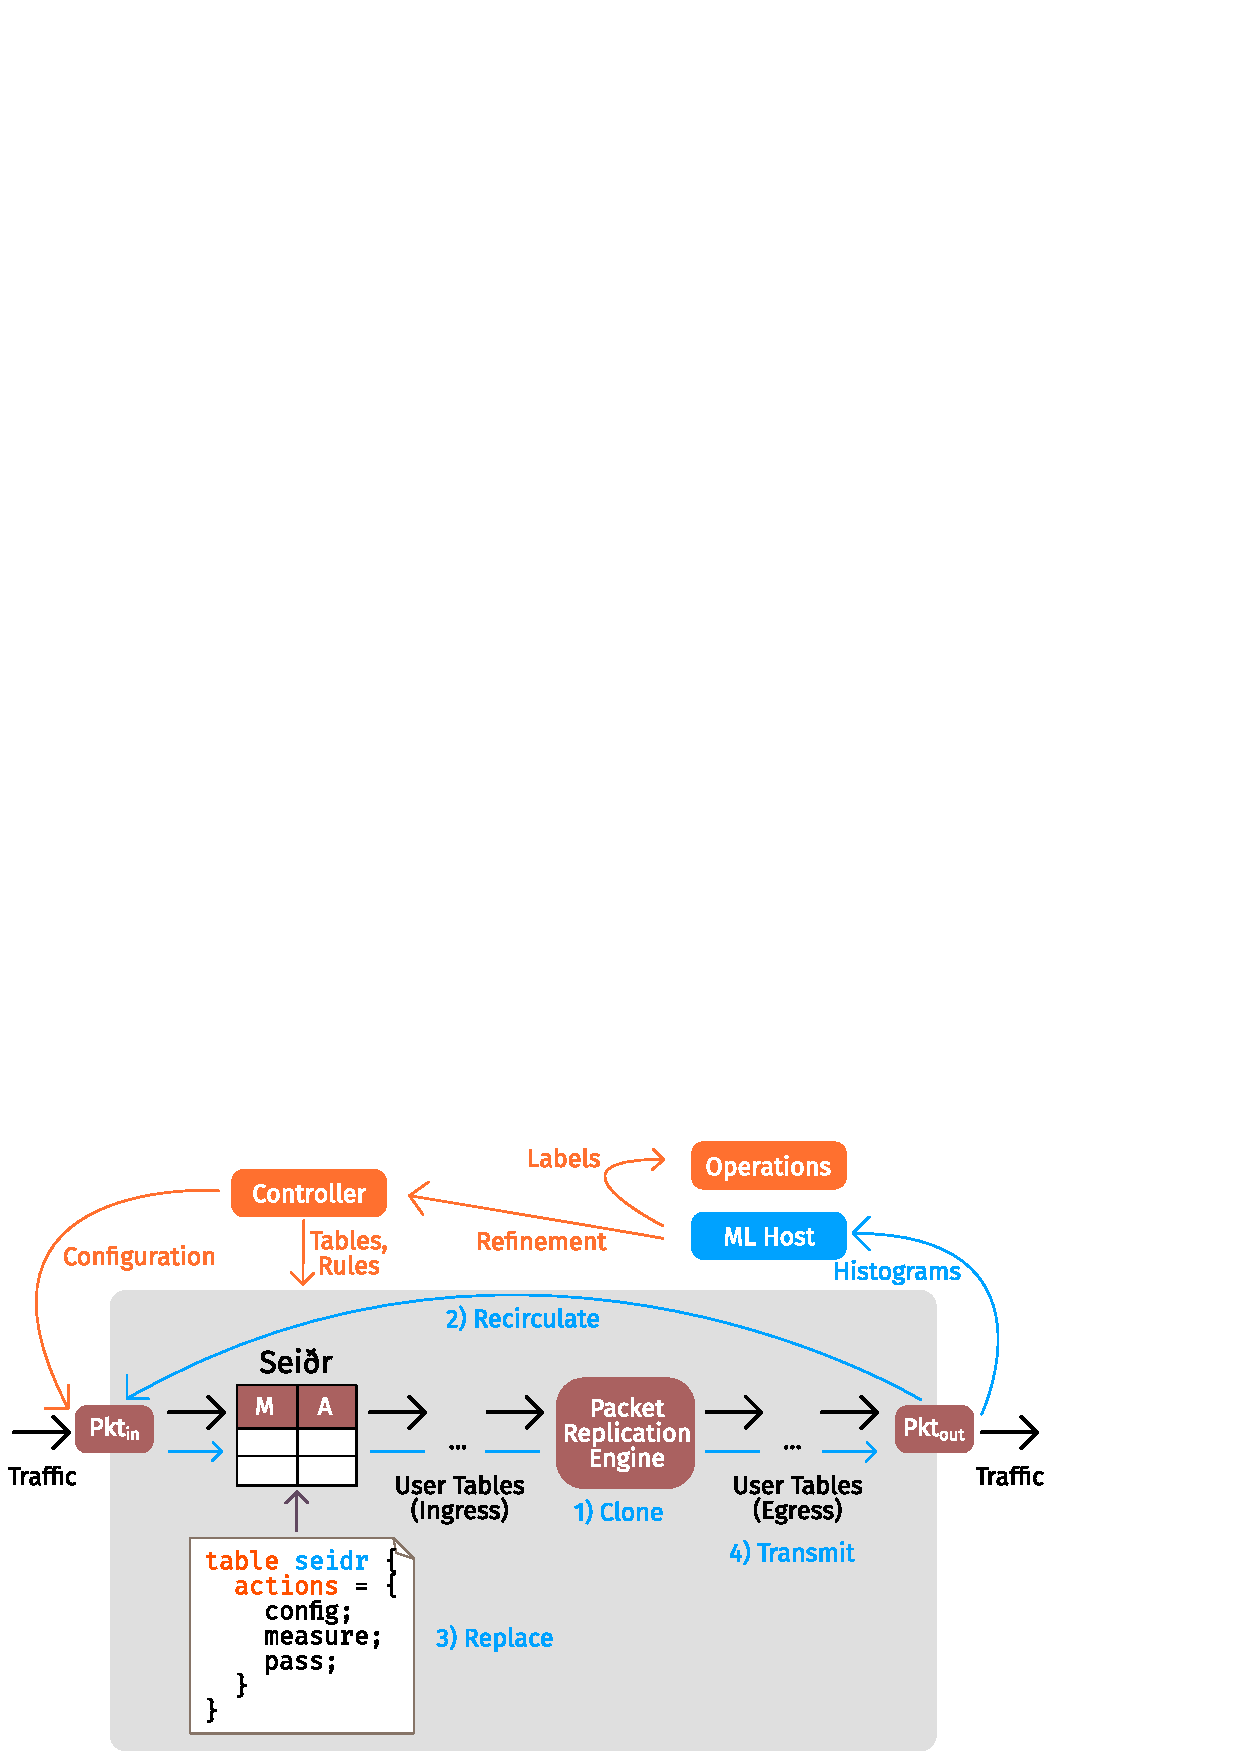
\includegraphics{diagrams/seidr/dp-arch-diagram.pdf}}
    \caption{\seidr{}'s integration with a PSA-compatible~\cite{p4-psa} dataplane.}
    \label{fig:arch}
\end{figure}

% Let's show them a histogram datastructure would look like purely with registers and how would a P4 action populate it - pseudocode or P4 snippet would be nice.

Although packet timing information is useful in understanding network and flow behaviour, without volume or packet rate reduction it is prohibitively expensive for hosts to handle each packet.
Histogramming acts as the \emph{aggregation step} which makes this class of analysis feasible in high-speed networks.
\Cref{fig:arch} demonstrates how \seidr{}, installed as an additional table in any P4 program, records and transmits inter-arrival time histograms.
The format for these histogram packets is outlined in \cref{fig:seidr-headers}; we choose to store individual buckets as \mintinline{rust}{u16}s, and the number of buckets in any histogram is fixed at compile time.
We set this to \num{100} buckets per histogram.
Packets traverse a table which requires \num{3} actions to be implemented:
\begin{enumerate}
    \item \mintinline{rust}{config} reads any matched packets as a \mintinline{rust}{seidr_cfg_t} of type \mintinline{rust}{SET_}\{ \mintinline{rust}{MIN}, \mintinline{rust}{MAX}, \mintinline{rust}{DST}, \mintinline{rust}{SRC}, \mintinline{rust}{LEN} \} by using the P4 parser.
    These update registers \numrange{1}{5} in \cref{tab:registers}, dropping any matched packets.
    
    \item \mintinline{rust}{measure} calculates the inter-arrival time, update per-flow histograms, and transmits finished histograms to the correct host. We describe its operation in \cref{alg:measure}.
    
    \item \mintinline{rust}{pass} ignores packets, and is the default action.
\end{enumerate}
Constructing \seidr{} in this manner allows the control plane to install rules to enable/disable runtime reconfiguration as needed, and to monitor as many or as few flows as desired (\ie, using wildcard rules, or exact matching).

The PSA does not have any mechanisms for generating new packets.
To circumvent this, any packet which would complete a histogram is tagged for cloning at the end of the ingress pipeline, and recirculation at egress (\cref{algline:recirc}).
This truncated copy returns to \seidr{}'s table, where we enable the relevant headers, change L2/3 fields, and write out the histogram contents (\crefrange{algline:rewrite-start}{algline:rewrite-end}).
The P4 deparser outputs the new protocol stack at egress, and transmits the histogram UDP packet into the network.
Event-driven architecture proposals~\cite{DBLP:conf/hotnets/IbanezABM19} may allow a more natural means of packet generation.

\begin{figure}
\centering
\begin{subfigure}{0.45\linewidth}
\centering
\adjustbox{max width = 0.6\linewidth}{
\begin{minipage}{\linewidth}
\begin{minted}[escapeinside=||]{rust}
|\textbf{\textcolor{Keyword}{header}}| seidr_cfg_t {
    bit<8> function;
    bit<144> payload;
}
\end{minted}
\end{minipage}
}
\end{subfigure}
\begin{subfigure}{0.45\linewidth}
\centering
\adjustbox{max width = 0.6\linewidth}{
\begin{minipage}{\linewidth}
\begin{minted}[escapeinside=||]{rust}
|\textbf{\textcolor{Keyword}{header}}| seidr_t {
    bit<128> src_ip;
    bit<128> dst_ip;
    bit<16> src_port;
    bit<16> dst_port;
    bit<16> eth_type;
    bit<BUCKETS * 16> histo;
}
\end{minted}
\end{minipage}
}
\end{subfigure}
\caption{P4 headers for \seidr{} configuration and histograms.}\label{fig:seidr-headers}
\end{figure}

\begin{algorithm}
% \vspace{-0.25cm}
% \DontPrintSemicolon
\KwData{5-tuple, P4 metadata, P4 headers, Registers}
h $\leftarrow$ hash(5-tuple)\;
index $\leftarrow$ BUCKETS * h\;
owner $\leftarrow$ HistoOwner[h]\;
\uIf{metadata.packet\_path = RECIRCULATE}{
    headers.tcp.valid $\leftarrow$ false\label{algline:rewrite-start}\;
    headers.udp.valid $\leftarrow$ true\;
    headers.seidr.valid $\leftarrow$ true\;
    copy 5-tuple into headers.seidr\;
    rewrite headers.ip, headers.udp using HistoSrc/Dest\;
    headers.seidr.histo $\leftarrow$ HistoData[index..]\;
    truncate payload\;
    zero out registers: BucketCount, HistoOwner[h], HistoData[index..]\;\label{algline:rewrite-end}
}
\ElseIf{owner = 0 \textbf{or} owner = 5-tuple}{\label{algline:owner-check}
    HistoOwner[h] $\leftarrow$ 5-tuple\;
    iat $\leftarrow$ LastTimestamp - metadata.mac\_ingress\_time\;
    \If{iat $\ge$ Min \textbf{and} iat $\le$ Max}{
        bucket $\leftarrow$ BUCKETS * (iat - Min) / (Max - Min)\;
        HistoData[index + bucket] $\leftarrow$ HistoData[index + bucket] + 1\;
        BucketCount[h] $\leftarrow$ BucketCount[h] + 1\;
        \If{BucketCount[h] = Len}{
            mark packet for cloning and recirculation\label{algline:recirc}\;
        }
    }
}

\caption{Histogram update and transmission.}\label{alg:measure}
\end{algorithm}

In the event of hash collision (\cref{algline:owner-check}), we ignore packets outside of the tracked flow to ensure that data is accurate.
As later processing and classification directly affect what decisions are made by operators or automatically taken by a policy (possibly leading to incorrect flow limits, QoS, \emph{etc.}), avoiding corruption/cross-contamination of operational data is paramount.
To gain collision resistance, Robin Hood hashing could be used up to a maximum distance in the table, treating a zeroed owner as empty and an illegal source IP as a tombstone value.

\begin{table}
    \centering
    \caption{Register map (Datatype, Amount) for an $h$-bit hash.}
    \resizebox{\linewidth}{!}{\begin{tabular}{@{}ccccccccc@{}}\toprule
        Min & Max & Length & HistoSrc & HistoDest & BucketCount & LastTimestamp & HistoOwner & HistoData \\ \midrule
        \mintinline{rust}{u16} & \mintinline{rust}{u16} & \mintinline{rust}{u16} & \mintinline{rust}{u16 + u128} & \mintinline{rust}{u16 + u128} & \mintinline{rust}{u16} & \mintinline{rust}{u64} & \mintinline{rust}{3 * u16 + 2 * u128} & \mintinline{rust}{BUCKETS * u16} \\
        1 & 1 & 1 & 1 & 1 & $2^h$ & $2^h$ & $2^h$ & $2^h$ \\ \bottomrule
    \end{tabular}}
    \label{tab:registers}
\end{table}

% Basic Logic:
% \begin{itemize}
%     \item table 1: three actions
%     \begin{itemize}
%         \item config: set R1 or R2 (controller installs rule matching a specific port/ip combo)
%         \item measure: take ingress timestamp from metadata, do stuff, write into lasttime, add to bucket and total if within bounds
%         \item pass (default)
%     \end{itemize}
%     \item then pass onto rest of tables
%     \item Why do it this way? can make it all or nothing through control plane.
%     \item How to write and send packet? Same trick as ESNET? (recirc w/ custom metadata to transform pkt)
% \end{itemize}

% ?? NOTE: See PSA \cite{p4-psa} for register format. Some papers, like Dapper, suggest that hash tables should be possible? That would work out very well in our benefit.

% ?? What is configurable? Min, max of the histogramming range

This design allows runtime configuration of all aspects save for the bucket count; at runtime, the only way to increase bucket resolution is to examine a smaller region of IATs.
While in theory this could be configured below a maximum compiled into the firmware, the difficulties introduced in classification/data processing make this infeasible.
Unless using stream-capable classifiers such as LSTMs~\cite{DBLP:journals/neco/HochreiterS97}, changing the input size requires retraining from scratch since new neuron weights must be added and structural properties of the input data change.
Increasing the bucket count requires new firmware installation, as many dataplane P4 implementations cannot allocate variable-length stores due to the lack of a dynamic allocator.

\begin{figure}[t]
    \centering
    \begin{subfigure}[t]{0.49\linewidth}
        \centering
        \resizebox{\linewidth}{!}{\includegraphics{plots/seidr/dt-cubic-1000-app.pdf}}
        \subcaption{TCP Cubic}
        \label{fig:cubic-hist-app}
    \end{subfigure}
    \begin{subfigure}[t]{0.49\linewidth}
        \centering
        \resizebox{\linewidth}{!}{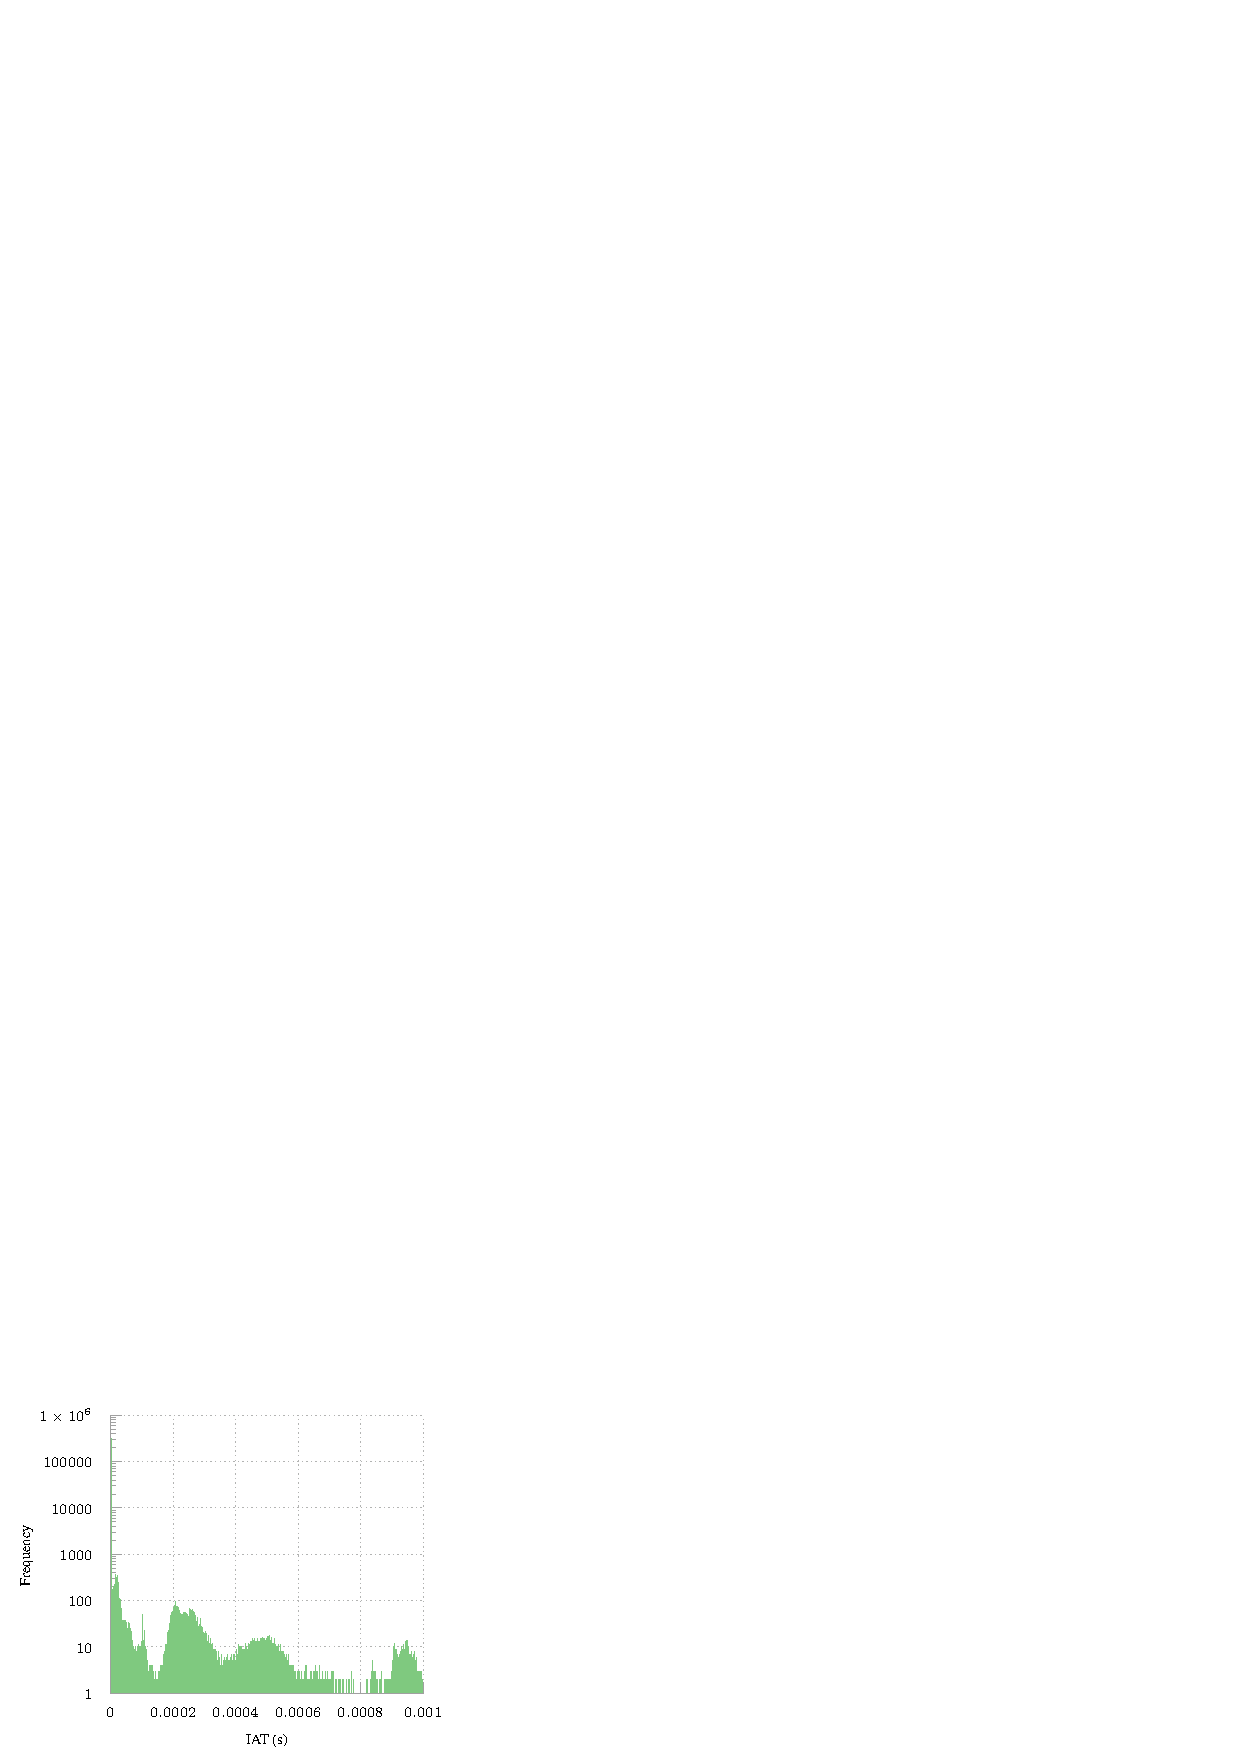
\includegraphics{plots/seidr/dt-bbr-1000-app.pdf}}
        \subcaption{TCP BBR}
        \label{fig:bbr-hist-app}
    \end{subfigure}
    \caption{Example dataplane histograms showing visible differences in inter-arrival times of selected TCP flavours. Our ML solutions are trained to programmatically identify such differences.}
    \label{fig:tcp-hist-app}
\end{figure}

As an example of dataplane-generated histograms, \cref{fig:tcp-hist-app} shows the distribution of inter-arrival times between two TCP congestion control algorithms. The visible differences are programmatically identified using our ML algorithms.

\subsection{Accurate, Precise and High-Resolution Timestamping}

Precise timestamps are critical when detecting temporal properties of flow behaviour, such as microbursts or inferring flow congestion control algorithms.
It is especially important in high speed (\SI{100}{\giga\bit\per\second}) networks, where there can be as little as \SI{6.7}{\nano\second} between packets that need to be analysed.
With a Linux-based software solution (\eg, reading packets from a link with \emph{tcpdump}), the Linux kernel can only provide microsecond-level accuracy with precision in the order of \SI{100}{\micro\second}~\cite{kundel2020p4sta}.
DPDK improves on this, increasing the accuracy to \SI{100}{\nano\second} in the best case~\cite{primorac2017measure}.
However, today's dataplane devices (\eg, Netronome SmartNICs, NetFPGA SUME) allow nanosecond-accurate timestamps to be retrieved from the \emph{Media Access Control} (MAC) modules with a precision of \SI{10}{\nano\second}~\cite{kundel2020p4sta}, a timestamp property \seidr{} relies upon.

% Some platforms provide picosecond-level precision and many solutions allow time synchronisation between multiple devices using the IEEE 1588-2002 (Precision Time Protocol) standard.



\section{TCP congestion control classification}\label{sec:seidr-tcpcc}


% We present an example of first-stage analysis performed for each flow and each packet---stateful TCP analysis.
% This includes numerous metrics which are considered standard when measured at connection endpoints, yet are difficult or invite numerous issues when performed in the network (of which we include a discussion on drawbacks and, curiously, benefits).
% The introduction of accurate timestamps allows us to explore rate-monitoring at a per-packet level, a new view of flow behaviour which may enable flow and hardware characterisation.

% \subsection{Per-Packet Rate Monitoring}

% \begin{figure*}
%     \centering
%     \begin{subfigure}[t]{0.49\linewidth}
%         \centering
%         \resizebox{0.5\linewidth}{!}{
% 	    \begin{tikzpicture}
%     		[packet/.style={draw, fill=uofgsunshine}]
% 		    \node[packet] (p1) {$p_1$: 1500B};
% 		    \node[packet, right= 1cm of p1] (p2) {$p_2$: 800B};
		
% 		    \node at ($(p1.south west) - (0,1)$) (t1) {$t_1$};
% 		    \node at ($(p2.south west) - (0,1)$) (t2) {$t_2$};
		
% 		    \draw[-, dotted] (t1.north)--(p1.south west);
% 		    \draw[-, dotted] (t2.north)--(p2.south west);
		
%     		\draw[<->] (t1.north) -- node[below]{$\mathit{dt}$} (t2.north);
% 	    	\draw[<->] ($(t1.north) + (0,0.2)$) -- node[above]{$s$} ($(t1.north) + (1.8,0.2)$);
% 		    \draw[<->] ($(t1.north) + (1.8,0.2)$) -- node[above]{$g$} ($(t2.north) + (0,0.2)$);
% 	    \end{tikzpicture} 
% 	}
%     \caption{\centering Per-packet rate, visualised. Note that $p_1$ and $p_2$ are not necessarily packets from the same flow.}
%     \label{fig:per-packet-rate}
%     \end{subfigure}
%     \begin{subfigure}[t]{0.49\linewidth}
%     \centering
%     \resizebox{0.9\linewidth}{!}{
% 		\begin{tikzpicture}
% 		[packet/.style={draw, fill=uofgsunshine}]
% 		\node[packet] (p1) {$p_1$: 1500B};
% 		\node[packet, right= 1cm of p1] (p2) {$p_2$: 800B};
% 		\node[right= 1cm of p2] (p3) {...};
% 		\node[packet, right= 1cm of p3] (p4) {$p_{n-1}$: 1500B};
% 		\node[packet, right= 1cm of p4] (p5) {$p_n$: 1500B};
		
% 		\node at ($(p1.south west) - (0,1)$) (t1) {$t_1$};
% 		\node at ($(p2.south west) - (0,1)$) (t2) {$t_2$};
% 		\node at ($(p4.south west) - (0,1)$) (t4) {$t_{n-1}$};
% 		\node at ($(p5.south west) - (0,1)$) (t5) {$t_{n}$};
		
% 		\draw[-, dotted] (t1.north)--(p1.south west);
% 		\draw[-, dotted] (t2.north)--(p2.south west);
% 		\draw[-, dotted] (t4.north)--(p4.south west);
% 		\draw[-, dotted] (t5.north)--(p5.south west);

%         \draw[<->] ($(t2.south) + (0,-0.25)$) -- node[above]{$s$} ($(t2.south) + (6.25,-0.25)$);
%         \draw[<->] ($(t2.south) + (6.25,-0.25)$) -- node[above]{$g$} ($(t5.south) + (0,-0.25)$);
% 		\draw[-, thick] ($(t2.south) - (0,0.5)$) -- node[below]{$W$} ($(t5.south) - (0,0.5)$);
% 		\end{tikzpicture} 
% 	}
%     \caption{\centering Sliding window rate, visualised. Rate estimates are computed using the sizes of the last $W$ packets seen in the current flow. Packets $p_2$ and $p_{n-1}$ belong to the same flow, but $p_n$ is not assumed to.}
%     \label{fig:sliding-window-rate}
%     \end{subfigure}
%     \caption{Comparison of per-packet and sliding window rates. The lengths of packets and inter-packet gaps are not to scale, and are purely demonstrative.}
%     \label{fig:pr-vs-slide}
% \end{figure*}

% Associating each packet with a high-resolution timestamp allows us to introduce the notion of a \emph{per-packet rate}.
% Assuming a packet with size $p$ arrives at time $t_1$ and is followed by another packet (potentially from another flow) which arrives at $t_2$, we measure $\mathit{dt}=t_2-t_1$ for this packet.
% Supposing this first packet spends time $s$ on the wire and assuming that the inter-packet gap $g$ is negligible compared to the length of a packet, then $\mathit{s} = \mathit{dt} - g \approx \mathit{dt}$.
% This packet then has a point rate, $r$:
% \begin{equation}
%     r = \frac{p}{s} \approx \frac{p}{\mathit{dt}}
% \end{equation}
% \Cref{fig:pr-vs-slide} demonstrates how this timing information arises, contrasted with sliding-window rate measurements taken over a longer time period.
% This assumes almost back-to-back traffic, which is realistic in our deployment environment, but to the best of our knowledge no programmable switches expose the timestamp at which the final bit of a packet has been ingested.
% Such a timestamp would allow exact measurement of $s$.

% % ?? we need to be clear about the unintuitive nature of these measurements, include a quick sketch proof which shows that the weighted average of a set of point rates is analytically identical to the sliding window rate/throughput taken over the same period of time.
% While this is an interesting measure to associate with each packet, considering how best to view such rates in aggregate can be counter-intuitive.
% Viewing these rates as time series data reveals interesting distributional characteristics which disagree starkly with our understanding of a flow's rate---for instance, clusters which suggest a different mean.
% Suppose we have a set of measurement indices $C$ with no gaps captured between $t$ and $t'$, partitioned into flows $C = F_1 \cup \dots \cup F_p$.
% To correctly combine a set of point measurements for a flow $F_i$ into an average rate $\overline{r}_{F_i}$, we compute:
% \begin{equation}
%     \overline{r}_{F_i} = \frac{\sum_{a \in F_i} \mathit{dt}_a r_a}{\sum_{c \in C} \mathit{dt}_c}.
% \end{equation}
% In the instance that only one flow is captured (\emph{i.e.}, $F_i = C$), this is a weighted average over point rates, using the $\mathit{dt}$ measured between each packet and the next packet in the same flow as its weight.
% Similarly, this is analytically equivalent to the sliding-window rate measured over the same set of packets:
% \begin{equation}
%     \frac{\sum_{a \in F_i} \mathit{dt}_a r_a}{\sum_{a \in F_i} \mathit{dt}_a} \simeq \frac{\sum_{a \in F_i} p_a}{t' - t}.
% \end{equation}
% % \begin{proof}
% % Given a set of contiguous measurements from the same flow $S \subseteq \mathbb{Z}$, admitting $p_s$, $r_s$, $\mathit{IAT}_s$ and $t_s$, the weighted average of point rates is then
% % $$
% % \overline{r}_S = \frac{\sum_{s \in S} \mathit{IAT}_s r_s}{\sum_{s \in S} \mathit{IAT}_s}
% % $$
% % The sliding-window average:
% % $$
% % \overline{r}_S = \frac{\sum_{s \in S} \mathit{IAT}_s r_s}{\sum_{s \in S} \mathit{IAT}_s}
% % $$
% % \end{proof}

% We assume that inter-packet gaps will be negligible (\emph{i.e.}, that the link is never in a state of very low utilisation), due to typically high utilisation on a WAN.
% % Similarly, we need to discuss the effects of selective monitoring or an abundance of UDP/ICMP traffic (which will distort $dt$s).
% However, this assumption can be distorted if selective TCP flow monitoring is used, or if UDP/ICMP traffic is overabundant; both these scenarios create larger gaps between TCP packets of interest, inflating $g$ to the point where it is comparable in size to $s$.
% This has an impact on our notion of per-packet rates, but not inter-arrival times or other such dependent metrics.
% The effect is small on sliding window rates, particularly at larger window sizes.
% ?? Justify. On paper, it looked like error term was O(1/n), O(g) for an n packet window.


% \section{Inter-Arrival Time}

% Having assigned each packet in a flow with a nanosecond-accurate timestamp ?? tbc

\Cref{fig:tcp-hist-app} suggests that a notable use-case for this type of measurement is \emph{congestion control algorithm} (CCA) detection.
In a TCP connection, each machine is free to choose the CCA it uses to send bytes, and thus how it responds to network congestion signals.
This choice is local, and so is invisible to the other machine (and the network).
In datacentre networks, operators choose these to ensure optimal behaviour.
In a transit network or large WAN however, these hosts (and thus the CCAs in use) are outside the control of network operators, which introduces difficulties when CCA interactions lead to \emph{unfairness}.
Consider the recent (and widespread) introduction of \emph{TCP BBR}~\parencite{DBLP:journals/queue/CardwellCGYJ16}.
\emph{BBR} is a delay/model-based CCA which converges on a fair share of bottleneck bandwidth by reducing its rate if the round-trip time increases, while periodically attempting to increase send rate to account for path/load changes.
However, \emph{BBR} traffic can consume \SI{40}{\percent} of link capacity when multiplexed with loss-based CCAs, regardless of the number of competing flows~\parencite{DBLP:conf/imc/WareMSS19}. 
When ensuring fair transit to all flows, this is hardly a desirable outcome; in fact, it's one which may frustrate clients or violate SLAs.

A curious property of \emph{BBR}'s algorithm which sets it apart from other variants is that packet transmission is \emph{timer-based}.
\texttt{send(packet)}, as defined in the canonical algorithm, asks that on transmission of a packet, the sender should wait for the estimated time that packet would take to reach the recipient.
For instance, at an estimated bottleneck bandwidth of \SI{8}{\mega\bit\per\second}, a \SI{1024}{\kilo\byte} packet would hold back the next packet in the flow until \SI{976.6}{\micro\second} had elapsed.
When packet sizes remain similar this causes strongly periodic behaviour, while mode switches in the \emph{BBR} algorithm cause these periodic bands to shift up or down accordingly.
This effect is stronger than in existing loss- and delay-based algorithms which remain intrinsically tied to the notion of a congestion window (where release of buffered packets follows the receipt of ACK messages).
As a result, timing behaviour of past CCAs may be influenced by (the lack of) packet pacing, periodic components might be made noisier by jitter along the return path, or the behaviour of the receiver might add further noise.

This high-level analysis of \emph{BBR} gives us a strong feature to use as the basis for classification: the \emph{inter-arrival times} (IATs) for each packet in a flow.
We have two options for processing this for classification: we may use a compressed, fixed-size representation such as histograms to capture the aggregate distribution, or we may attempt to capture structural behaviour by using a variable-length stream of IATs.
In many networks, the data and packet rate reduction offered by the former is required to make this possible.
Indeed, in-switch aggregation has seen great success in aiding ML for training~\parencite{DBLP:conf/isca/LiLYCSH19}, and direct execution~\parencite{DBLP:conf/hotnets/XiongZ19}.
We make use of the following standard classification algorithms on a fixed-size representation to attempt to single out the CCA in use:

\begin{itemize}
    \item \emph{$k$-Nearest Neighbours ($k$-NN)}. A simple and well-understood classifier which assigns labels based on the closest members of the training corpus (\ie, by the $L_2$ metric). Linear memory cost in amount of training data, and no training cost other than loading all data points, but capable of learning complex decision boundaries on fixed-length input.
    
    \item \emph{Convolutional Neural Networks (CNNs)}. A neural network approach which learns convolution kernels to classify fixed-length data, particularly when recognising spatial features. Memory cost is fixed for a given architecture irrespective of training data, with a high training cost.
\end{itemize}
% \fakepara{Long Short-Term Memory~\parencite{DBLP:journals/neco/HochreiterS97} units (LSTMs)} A class of recurrent neural network used for stream classification, forecasting, and prediction of variable-length data. Memory cost is fixed, with longer training times (and more data required) than similarly sized CNNs.
% Of these, we apply $k$-NN and CNNs to histograms of packet IATs, and LSTMS to raw IAT streams.

When examining $k$-NN classifiers, we measured accuracy across choices of $k \in \left[2, 8\right]$.
We found $k=2$ to be the most effective choice with our input data using the $L_2$ metric.
Our CNN architecture is described in \cref{tab:cnn-arch}, using ReLu activation and $1 \times 1$ stride in convolutional layers unless stated otherwise.
Training occurred over 5 epochs using the Adam optimiser with categorical cross-entropy as a loss metric, and a batch size of \num{64} histograms (\num{8} for full sequences due to the smaller data volume).
For \emph{BBR vs.\ Cubic}, the complete model consists of \num{104898} 32-bit floating-point parameters (\SI{409.76}{\kibi\byte}), while the full classification task adds a further \num{130} parameters (\SI{0.51}{\kibi\byte}).

\begin{table}
    \centering
    \caption{CNN architecture for \num{100}-entry histograms.}
    \resizebox{0.7\linewidth}{!}{\begin{tabular}{@{}cccc@{}}\toprule
        Layer & Nodes/Filters & Filter Size & Output Dimension \\ \midrule
        Conv2D & 32 & $(3 \times 1)$ & $(98 \times 1 \times 32)$ \\
        MaxPool & --- & $(2 \times 1)$ & $(49 \times 1 \times 32)$ \\
        Conv2D & 64 & $(3 \times 1)$ & $(47 \times 1 \times 64)$ \\
        MaxPool & --- & $(2 \times 1)$ & $(23 \times 1 \times 64)$ \\
        Conv2D & 64 & $(3 \times 1)$ & $(21 \times 1 \times 64)$ \\
        Flatten & --- & --- & \num{1344} \\
        Dense & 64 & --- & \num{64} \\
        Dense (Softmax) & $n_\mathit{classes}$ & --- & $n_\mathit{classes}$ \\
        \bottomrule
    \end{tabular}}
    \label{tab:cnn-arch}
\end{table}


\section{Evaluation}\label{sec:seidr-evaluation}
%Traffic is played back from hosts via Tcpreplay at a bandwidth assigned uniformly from a `good' or `bad' distribution, each using the same pcap file with source and destination IP addresses rewritten.

This work is most naturally compared against Marl, introduced by \textcite{DBLP:journals/eaai/MalialisK15}, the state-of-the-art in \gls{acr:rl}-based \gls{acr:ddos} prevention.
We are most interested in seeing how their approach contrasts with the new agent designs across different topologies and workloads.
Different network environments will also impose different levels of host density, where popular web servers may have orders of magnitude more clients than egress points from their network---I aim to show how these characteristics affect performance and learning rate.
Marl is known to outperform the AIMD~\parencite{DBLP:journals/ton/YauLLY05} strategy, yet the state of the art has long since moved on.
To paint a more current picture, I compare this work against an effective modern approach, \emph{SPIFFY}~\parencite{DBLP:conf/ndss/KangGS16}.
SPIFFY tests a proportion of flows by routing them through an alternate path with higher bandwidth, observing how their speed changes some time later.
This comparison lets us position our new agent designs against the state of the art, observing that SPIFFY has a similar mode of interaction to \gls{acr:rl}-based systems (taking action, observing an effect, and acting once again) and does not rely on protocol characteristics or signatures.
In reimplementing SPIFFY, I make the simplifying assumption that a suitable unused path exists (with identical bandwidth to the server's link).
\qty{10}{\percent} of active flows were tested at a time (according to the authors' observation that there is a factor of \qty{10}{\times} difference between the ideal and achieved bandwidth expansion), excluding flows below \qty{50}{\kilo\bit\per\second} and requiring a \qty{3}{\times} expansion from legitimate flows, making a judgement after \qty{5}{\second}.

To test this, I made use of both traffic models introduced in \cref{sec:a-new-normal} (Opus and \gls{acr:tcp}), both topologies discussed below (1-dest vs.\ Fat-Tree), and vary the amount of hosts typically communicating over each agent's ingress/egress node.
Additionally, these new models were evaluated in multi-agent mode (\emph{separate}, no model sharing), and in single-agent mode (\emph{single}, zero-cost perfect information sharing).
In each case, the algorithm's performance was averaged over \num{10} episodes of length \num{10000} timesteps (setting each agent's $\wvec{}=\mathbf{0}$ between episodes).
Host allocations at the beginning of each episode were generated pseudorandomly to ensure fairness between episodes---a host is malicious with probability $\operatorname{P}\left(\mathit{malicious}\right)$, and is benign otherwise.
Benign hosts generate traffic according to either \cref{sec:tcp-http-traffic-model,sec:udp-opus-traffic-model} depending on the experiment, while malicious hosts generate traffic as described in \cref{sec:attack-traffic-model} (both at experiment-dependent rates).

All experiments were executed on Ubuntu 18.04.2 LTS (GNU/Linux 4.4.3-040403-generic x86\_64), using an Intel Core i7-6700K (\qtyproduct[product-units=single]{4 x 4.2}{\giga\hertz}) which had \SI{32}{\gibi\byte} of \gls{acr:ram}.
%All code underpinning these findings is available on a public repository\footnote{\url{https://github.com/FelixMcFelix/rln-dc-ddos-paper}}.
%All code underpinning these findings is available on a public repository.\footnote{Private until publication.}

\subsection{Single destination}\label{sec:single-dest}
%?? Move description of tree topol to here.
The network is tree-structured, where one server $s$ connects through a dedicated switch to $k$ team leader switches, each connected to $\ell$ intermediate switches, which in turn each connect to $m$ egress switches.
We then have $N_{\mathit{hosts}} = k \ell m n$.
\Cref{fig:marl-topol} demonstrates this.
%Although \citeauthor{DBLP:journals/ccr/MahajanBFIPS02a}, the originators of this topology, make it clear that it exists as a fairly unrepresentative example \cite{DBLP:journals/ccr/MahajanBFIPS02a}, it remains the case that such a network topology allows for functional testing, and indeed is illustrative of one way in which attack traffic might aggregate in the network.
%It is hard, however, to argue its relevance to specific classes of victim or to reason about the interactions it might have with dependent applications.
%We aim to address this through \cref{sec:performance-in-an-emulated-environment}.
The network topology was configured using $k=2$ teams, $\ell=3$ intermediate nodes per team, $m=2$ agents per intermediate node, and $n \in \{2, 4, 8, 16\}$ hosts per learner.
This is a slight simplification of \Textcite{DBLP:journals/eaai/MalialisK15}'s \textquote{online} experiment, choosing fewer teams but remaining as a single server with a fan-out network.
%The algorithm parameters were set at $\gamma=0$ (leading to opportunistic behaviour), $\alpha=0.05$, having linearly annealed $\epsilon=0.2 \rightarrow 0$ by $t=3000$.
%Benign and malicious hosts uploaded between \SIrange{0}{1}{\mega\bit\per\second} and \SIrange{2.5}{6}{\mega\bit\per\second} respectively, and hosts were redrawn at each episode's start with $\operatorname{P}(\mathit{malicious})=0.4$.
%$U_s$  $k \ell mn+2$ \si{\mega\bit\per\second}.
%The performance of each choice of $n$ was averaged over \num{10} episodes of length \num{10000} timesteps (setting each agent's $\wvec{}=\bm{0}$ between episodes).
%Host allocations were generated pseudorandomly to ensure fairness between choices of $n$.
%These parameter choices match those of the original study to enable direct comparison, and are (to the best of our knowledge) arbitrary, but we justify our range of $n$ as capturing increasing scales of host activity.

\begin{figure}
	\centering
	\resizebox{0.9\linewidth}{!}{\begin{tikzpicture}[
	texts/.style = {text=black},
	labeltexts/.style = {text=uofgsandstone},
	treeline/.style = {draw=uofgburgundy},
	treenode/.style = {texts, circle, centered, fill=white, treeline},
	load/.style = {fill=uofgcobalt},
	loadhide/.style = {fill=uofgcobalt!40!white},
	external/.style = {fill=uofgrust},
	externalhide/.style = {fill=uofgrust!40!white},
	hideline/.style = {draw=uofgsandstone!40!white},
	hidenode/.style = {treenode, hideline},
	grow'=right
]
	\node[treenode, label={[texts]above:Server}] (root) {}
	child [treeline] { node [treenode, label={[texts]above:Core}] (sswitch) {}
		child [treeline] { node [treenode, label={[texts]above:Leader}] (teaml) {} 
			child [treeline] { node [treenode, label={[texts]above:Intermediate}] (inter) {}
				child [treeline] { node [treenode, load, label={[texts]above:Agent/Egress}] (agent) {}
					child [treeline] { node [treenode, external] (extern) {}
						child [treeline] { node [treenode, external, label={[texts]above:Host}] (host) {} }
						child [hideline] { node [hidenode, externalhide] (endhost) {} }
					}
				}
				child [hideline] { node [hidenode, loadhide] (endagent) {} }
			}
			child [hideline] { node [hidenode] (endinter) {} }
		}
		child [hideline] { node [hidenode] (endteaml) {} }
		edge from parent
		node[below, labeltexts] {$U_s$}
	};
	
	%\draw[-] (teaml) -- (endteaml);
	\node [labeltexts] (kdots) at ($(teaml)!0.5!(endteaml)$) {$\rvdots$};
	\node [labeltexts, right = -0.1cm of kdots] {$k$};
	\node [labeltexts] (ldots) at ($(inter)!0.5!(endinter)$) {$\rvdots$};
	\node [labeltexts, right = -0.1cm of ldots] {$\ell$};
	\node [labeltexts] (mdots) at ($(agent)!0.5!(endagent)$) {$\rvdots$};
	\node [labeltexts, right = -0.1cm of mdots] {$m$};
	\node [labeltexts] (ndots) at ($(host)!0.5!(endhost)$) {$\rvdots$};
	\node [labeltexts, right = -0.1cm of ndots] {$n$};
\end{tikzpicture}}
	\caption[Tree-structured network topology diagram for evaluating a single-destination network.]{
		Network topology diagram, showing how the server and its core switch's $k$ teams are structured, with $\ell$ intermediate routers per team, connected to $m$ agents which each moderate $n$ hosts beyond a single external switch.
		%	Empty nodes are considered to be internal.
		Red nodes are external, and each blue node hosts an agent.
		\label{fig:marl-topol}
	}
\end{figure}

\subsection{Multiple destinations}
The previous topology allows for direct comparison against the state-of-the-art, and indeed is illustrative of one way in which attack traffic might aggregate in the network.
It is hard, however, to argue its relevance to specific classes of victim or to reason about the interactions it might have with dependent applications.
In contrast, the fat-tree topology~\parencite{DBLP:conf/sigcomm/Al-FaresLV08} sees regular use in real-world data centres and scales well horizontally.
%?? Come up with description of fat-tree (multi-dest) topol.
%?? Why fat tree? regularly appears in modern datacentres.
%?? $k=4$ fat-tree , with one pod hosting two servers $s_0,s_1$.
We use a $k=4$ fat-tree, with one pod hosting two servers $s_0$ and $s_1$.
$n$ external hosts connect through each core switch (where agents are hosted), and communicate with $s_0, s_1$ uniformly randomly.
Both servers host identical services.
We set $n \in \{6, 12, 24, 48\}$ hosts per learner (keeping $N_{\mathit{hosts}}$ identical to each tier of the single-host topology), and restrict $U_{s_0} = U_{s_1} = U_s / 2$.

\subsection{Parameters}
The algorithm parameters were set at $\alpha=0.05$, linearly annealing $\epsilon=$ \num{0.2} $\rightarrow$ 0 by $t=$~\num{3000} in the case of Marl (\num{8000} actions per agent in the \emph{Instant/Guarded} models).

Benign hosts each occupied \qtyrange{0}{1}{\mega\bit\per\second}, and hosts were redrawn at each episode's start with $\operatorname{P}(\mathit{malicious})=$~\num{0.4}.
%The original introduction of this approach to direct-control reinforcement learning as introduced by \textcite{DBLP:journals/eaai/MalialisK15} fails to consider key cases: the absence of a suitable heuristic classifier $g(\cdot)$, disjoint ranges of traffic distribution (i.e., the presence of benign heavy-hitters), the accurate simulation of TCP-like behaviour (and its effects on collateral damage), and high densities of hosts at egress points.
%?? Why? ...
%Of these, the latter two are most deserving of a closer investigation, as they have stronger implications for wide-scale deployment.
%These are important issues, particularly when we consider real-world deployment.
%Heuristic estimates of traffic legitimacy come with computational cost and couple the reward function to the accuracy of the estimator, hosts often show diversity in their own traffic patterns (perhaps being multi-modal), and it is known that TCP is the most used transport protocol for Internet traffic \cite{DBLP:conf/saint/ZhangDJC09}.
%?? NEED TO VERIFY VOLUME OF CONGESTION-AWARE PROTOCOLS
Malicious hosts each sent \qtyrange{2.5}{6}{\mega\bit\per\second} when attacking \gls{acr:udp} traffic, though this was increased to \qtyrange{4}{7}{\mega\bit\per\second} when using \gls{acr:tcp}-like traffic (to meaningfully impact benign flows).
Given $n$ and $\operatorname{P}(\mathit{malicious})$, we see an expected malicious bandwidth \numrange{1.27}{1.87} and \qtyrange{2.03}{2.18}{\times} $U_s$ respectively.
%The expected fraction of $U_s$ consumed by each host is \SI{21.5}{\percent} for $n=2$, and \SI{2.84}{\percent} for $n=16$.
For these choices of $n$ in both topologies, we observe $N_{\mathit{hosts}} \in \left\{24, 48, 96, 192\right\}$, and an expected number of malicious hosts $\mathbb{E}\left[N_{\mathit{attackers}}\right] \in \left\{9.6, 19.2, 38.4, 76.8\right\}$.
For the largest choice of $n$, we see an expected total attack traffic $\mathbb{E}\left[V_{\mathit{attack}}\right] =$ \qtylist{334.05;422.4}{\mega\bit\per\second} for Opus and \gls{acr:http} traffic respectively.

$U_s$ was fixed at $N_{\mathit{hosts}}+2$ \unit{\mega\bit\per\second} (to account for burstiness), and each link had a delay of \qty{10}{\milli\second}.
All links had unbounded capacity, save for each server-switch.
These parameters match those of the original study to enable direct comparison, and many are (to the best of our knowledge) arbitrary, but I justify the range of $n$ as capturing increasing scales of host activity.

% \section{Related Work}\label{sec:related}
% %?? Try and compare my work here when possible?

\fakepara{DDoS Prevention}
\Textcite{DBLP:conf/lcn/BragaMP10} examine the detection of flooding DDoS attacks through \emph{self-organising maps}, using SDN to gather statistics effectively.
Many of their features aren't overly relevant, as their focus is not active defence or discovering \emph{which} hosts contribute to an attack.
%?? Actually talk about Marl (???) to appease reviewer \#1.
The closest available approach within this field is that of \textcite{DBLP:journals/eaai/MalialisK15} (whom we have positioned our work against), and their contribution in applying RL to the task of intrusion prevention is significant: their work helps to show the viability of live, adaptive, feedback-loop-like control of the network to detect and prevent DDoS attacks.
They create a tree overlay topology (subdivided into teams), where each agent applies packet drop to \emph{all} flows inbound to a protected server.
%?? Recap their flaws, since they've been cut form every other aspect.
Our results show that their technique underperforms at high host density and when congestion-aware traffic dominates---that their results do not demonstrate this suggests an evaluation driven purely by traces (rather than live application dynamics).

\emph{SPIFFY} \cite{DBLP:conf/ndss/KangGS16} aims to remedy transit-link attacks by observing how flows from each source respond to a sudden increase in available bandwidth.
\Citeauthor{DBLP:conf/ndss/KangGS16} realise that bots participating in an attack are often unable to match this bandwidth expansion (having already saturated the capacity of their outbound links), while legitimate flows typically speed up to match the new fair-share rate.
%Attackers must either be detected or reduce the throughput of each bot, increasing the cost of launching an attack.
%Unlike our approach (and due to the class of attacks it is designed to defend against), SPIFFY is intended to be deployed within ASes, although .
A weakness of their approach is that computing a route to measure bandwidth expansion on real networks can be costly (up to \SI{14}{\second} for the Cogent topology), and that the low expansion factors in real network can require more ``rounds'' of filtering.
By contrast, our approach takes a constant time to compute an action for a flow regardless of topology size.
Their assumptions about traffic response to such bandwidth expansion do not hold for constant bitrate flows (e.g., VoIP) and may not extend to HTTP DASH flows, both of which make up a sizeable proportion of network traffic.

\emph{Athena} \cite{DBLP:conf/dsn/LeeKSPY17} is a generalised SDN framework for intrusion detection, but has shown the use of a \emph{k-nearest neighbours} classifier to detect individual attack flows.
Although heavyweight (and proven to be effective compared with \textcite{DBLP:conf/lcn/BragaMP10}), their comparison against SPIFFY lacks the quantitative evidence required to understand how the system compares.
\Textcite{DBLP:conf/sp/SmithS18} use AS-level routing to tackle both transit-link and flooding-based attacks.
This view is taken due to the perceived cost of per-stream classification and inherent sensitivity to adversarial examples.
The approach is creative, relying upon BGP \emph{fraudulent route reverse poisoning} to preserve traffic to a target AS, but unlike SPIFFY the approach doesn't actually \emph{remove} the congestion.
Because of this, flooding-based attacks aren't fully alleviated.

%?? Abuses of RL 
\fakepara{RL in Networks}
Earnest, well-considered application of RL towards the challenge of intrusion prevention has seen comparatively little examination.
Past work treats the paradigm as a traditional classifier for anomaly detection \cite{shamshirband2014anomaly} and DDoS prevention \cite{DBLP:conf/mates/ServinK08}.
Given that the main strengths of RL techniques are the ability to control ongoing interaction and adapt by observing the concrete effects of actions, such works don't apply the rich literature on the subject to its fullest potential.

For categorising how RL fits into solving problems, we label works as direct- or indirect-control RL.
A \emph{direct-control} RL problem is one where the RL agent(s) learn optimal control over a set of actions as the \emph{primary} defence or decision-maker---requiring measurements, reward functions and action sets tailored for this purpose.
%We feel there is a shortage of work in this category at present, at least in the field of networks.
To date, the best-fitting example we have encountered is that of \textcite{DBLP:journals/eaai/MalialisK15}.
An \emph{indirect-control} RL problem is one where agents act in service to \emph{another technique} responsible for decision-making, optimising or generalising aspects of its operation beyond that of hand-coded heuristics.
A past example includes learning when best to share knowledge between \emph{hidden Markov model} anomaly detectors \cite{DBLP:conf/paisi/XuSH07}.
%The position of this work is weakened by its reliance on the problematic `DARPA99' dataset \cite{DARPA-IDD, DBLP:conf/cisda/TavallaeeBLG09, DBLP:conf/sp/SommerP10}, but the idea itself is well-treated and this acts as a driver for improvements in this direction.
This work is weakened by its reliance on the problematic `DARPA99' dataset \cite{DBLP:conf/sp/SommerP10}, but the idea itself is well-treated.
Outside of intrusion detection, there has been growing interest in the use of RL in data-driven networking, such as for intra-AS route optimisation \cite{DBLP:conf/hotnets/ValadarskySST17} and resource-constrained process allocation \cite{DBLP:conf/hotnets/MaoAMK16}.
\textcite{DBLP:conf/sigcomm/MaoNA17} employ client-side observations of network state and video performance with RL to optimise bitrate selection for multimedia streaming.
\emph{AuTO} \cite{DBLP:conf/sigcomm/ChenL0L18} employs deep RL to perform traffic optimisation.
Crucially, they find that the vast majority of flows are short-lived, requiring effective decisions in less than a millisecond.
To overcome the high latency of action computation via a neural network, two agents are trained, handling aspects of short and long flows respectively.
The first learns to optimise the flow size thresholds to demarcate long and short flows; these short flows are routed by ECMP.
The second agent makes bespoke decisions about routing, prioritisation etc.\ for each of the remaining long flows.


\section{Summary}\label{sec:seidr-conclustion}
We have presented \seidr{}, a dataplane assisted flow classification solution that can be used to detect fine-grained temporal flow behaviour. We have shown a PSA-compliant way to implement in-network data aggregation in the form of histograms, while using nanosecond-precision timestamping. Our in-network generated histogram datastructure (\eg, on per-flow packet inter-arrival times) has been presented as the input for various ML algorithms, including CNN and $k$-NN. We have shown with our extensive evaluation that \seidr{} can successfully tell apart TCP CCAs, in particular, it identifies BBR from its predecessors with over \SIrange{88}{96}{\percent} accuracy, while only consuming a maximum \SI{15.5}{\mebi\byte} of dataplane memory. We presented the trade-offs between training and inference times, memory requirements, and accuracy in the context of CNN and $k$-NN classifiers and shown that \seidr{} outperforms prior work by increasing classification accuracy on novel TCP CCAs, providing the ability to classify at very high traffic rates (in the order of \SI{10}{\tera\bit\per\second}).
Furthermore, we have identified a key temporal property of \emph{BBR} which allows its easy detection among other flows.
In the future, we aim to examine the use of \seidr{} towards microburst detection and diagnosis~\cite{DBLP:conf/sigcomm/ChenFKRR18} and for the identification of \emph{BBR}-like temporal properties of emerging UDP-based congestion-aware protocols, such as \emph{QUIC}.%~\cite{DBLP:conf/sigcomm/LangleyRWVKZYKS17}.

?? Through this chapter, we have discussed ..., lending credence to one of the claims in my thesis statement: \superrecallthesis{3}

\chapter{Scalable Flow Classification}\label{chap:seidr}

% \section{Motivation}
% \section{Sei\dh{}r Histograms}
% \subsection{Algorithm}
% \subsection{Packet Generation on PSA}
% \section{Use case: TCP CCA Detection}
% \subsection{Observable Differences}
% \subsection{Investigating the BBR Algorithm}
% \section{Methodology}
% \subsection{Testing Environments}
% \subsection{Data Collection/Generation}
% \subsection{ML Model Architecture}
% \section{Evaluation}
% \subsection{Device Memory Costs}
% \subsection{Bandwidth Costs}
% \subsection{CCA Detection Accuracy and Costs}

?? Problem statement: damn, all this ML is cool
?? We can do cool real-time analysis of operational Internet traffic
?? What do we do if we need more complex ML models: i.e., need to use LSTMs, or complex CNNs because we need to make use of complex temporal or structural features of data? We still need to get it to host machonies.
?? Okay... but in that case, how can we reduce data so that PPS and Gbps of data don't overwhelm the host, or that we lose lots of asid data and make poor decisions when we have many (or very fast) flows?

?? Relate some of this \emph{specifically} back to discussion of flow measurement in the dataplane in the INC use-cases? (i.e., considering all th below IPfix, sFLow, etc. etc.)
?? Try to relate some of the same problems.

There has been significant research and development on real-time analysis of operational Internet traffic.
Accurate flow characterisation (or \emph{classification}) can drive intrusion detection, detecting unusual or illegal patterns of network traffic, or to prioritize traffic for certain customers, to provide path-diversity as well as to mark Quality of Service (QoS) of various users and protocols~\parencite{DBLP:journals/ccr/BernailleTASS06,DBLP:conf/lisa/Roesch99}.
However, flow classification solutions today can usually only rely on sampled data provided by routers, such as sFlow, Netflow, or IPFIX, along with imprecise timing (\si{\micro\second} and \si{\milli\second}-level)~\parencite{rfc7011,rfc3954}.
While sampled, low-precision telemetry can be used to classify network traffic based on some flow properties (such as port and protocol numbers)~\parencite{DBLP:conf/iwcmc/RossiV10}, it cannot be used to classify based on fine temporal properties (\eg, identifying bursty flows and senders that can cause microbursts and buffer overflow on the network).

On the other hand, full-software solutions for traffic classification have been proposed by commercial vendors (\eg, Barracuda DPI\footnote{https://www.barracuda.com/glossary/deep-packet-inspection}), the open-source community (\eg, Snort~\parencite{DBLP:conf/lisa/Roesch99}, Zeek (formerly Bro)~\parencite{DBLP:conf/uss/Paxson98,zeek}), and the research community, with extensible feature sets and algorithms for classification~\parencite{DBLP:conf/icccn/HagosEYK18}.
Unfortunately, these software solutions designed for commodity hardware do not provide accurate timing of packets, and therefore make certain time-critical events hard or impossible to detect (\eg, microbursts~\parencite{DBLP:conf/sigcomm/ChenFKRR18} or congestion control properties~\parencite{DBLP:conf/icccn/HagosEYK18}).
Moreover, even the most sophisticated software solutions process packets orders of magnitude slower than current backbone traffic of large operators, making them unusable for large-scale operational analysis~\parencite{DBLP:journals/wpc/ParkA17}.

At the same time, programming and fast reconfiguration of network devices is being explored in all types of networks: datacenter and cloud networks, CDNs and WANs.
Specifically, with the recent developments of generalized dataplanes (\eg, the \emph{Portable Switch Architecture}~\parencite{p4-psa}), target devices (\eg, Barefoot Tofino and Netronome SmartNICs) along with the high-level programming languages presented for them (\eg, P4~\parencite{DBLP:journals/ccr/BosshartDGIMRSTVVW14}), operators can now express in-network functionality running on their devices, including accurate nanosecond-precision packet timing.
However, programming in-network services has its own challenges (\eg, restricted instruction sets, data types and memory), prohibiting the implementation of a fully in-network classification solution.

% To solve the aforementioned challenges, this paper presents an architecture that marries the precision timing and fast data aggregation capabilities of the dataplane with software classifiers that can run complex classification models due on a the reduced data rate.

To solve the aforementioned challenges, we present \seidr{}\sidenote{Pronounced ``SAY-ther''. ?? Explain naming?}, a dataplane assisted flow classification solution.
Our design philosophy of \seidr{} keeps functionality where it belongs: dataplane devices create accurately timestamped, aggregated data structures for our analysis, and we let a scalable software stack perform ML-based classification on commodity machines.\sidenote{?? Yeah this directly contradicts the main theme and line of reasoning of my thesis LMAO}
As in-network aggregation reduces the data rate by a factor of $\sim$\num{740}, our solution can analyse aggregated data from a total rate of \SI{10}{\tera\bit\per\second} original traffic using a single commodity processing machine.

As a concrete use-case, we look at fine dynamics of TCP congestion control algorithms.
Understanding and classifying them is important for network providers as inadequate choices have severe effects on transfer rates, especially in networks with high bandwidth-delay product~\parencite{DBLP:journals/queue/CardwellCGYJ16} and in networks where multiple congestion control algorithms are used~\parencite{DBLP:conf/imc/WareMSS19}. 
By using accurate congestion control diagnostics, operators will be able to infer sender problems (\eg, backlogged or application-limited senders), network inefficiencies (\eg, increased path latency and congestion), as well as receiver issues (\eg, delayed acknowledgements, small receiver windows) and fairness issues between delay-based and loss-based algorithms~\parencite{DBLP:conf/imc/WareMSS19}.

The contributions of this paper are summarized below:
\begin{itemize}
	\item A flexible dataplane-assisted architecture compatible with the \emph{Portable Switch Architecture} (PSA)~\parencite{p4-psa} that allows data aggregation in the form of histograms with nanosecond-accurate timing (\Cref{sec:architecture}),
	\item A high-accuracy method for telling apart timer-based (\eg, BBR) and cwnd-based TCP flavours using our system with machine learning algorithms (\Cref{sec:tcpcc}),
	\item An extensive evaluation of TCP congestion control classification using our solution (\Cref{sec:evaluation}).
\end{itemize}

The work presented in this chapter considers how \gls{acr:pdp} hardware can reduce input, though fine-grained, measurements into digests suitable for \gls{acr:ml} models running on host machines, and is based upon \citetitle{DBLP:conf/globecom/SimpsonCP20}~\parencite{DBLP:conf/globecom/SimpsonCP20}.
?? Then summarise contents from here...

?? Big open qs:
?? relevance of PSA digests? These can emit packets, no? These can emit an arbitrary struct to the ctl plane over P4Runtime API. Might be good if no digest support, . Digests have a few extra benefits: In some dataplanes can be emitted in egress. Is message fusion a possible downside? (unpredictable)
?? Maybe 2 options? Can be in-band or out-of-band. Digests are the out-of-band option, meanwhile in-band allows you to use dataplane to forward to accelerators like BrainWave (don't add extra load to ctl plane in this way?)

?? Header size limits are the other main constraint.
?? THis is probably not a problem with digests.
?? WHen emitting to dataplane, however? Will have plat-dependent limits on output. Header size limits, PHV limits, register access reqs that could prevent digest access? Need to mark in-progress histo emissions, progress for each, and emit bitslices spread over multiple egress pkts. Logic: CLONE LOOP WHile still pkts to write, block updates to histo if progress (1 bit?). Limitation: Histo emission freq must be reduced to prevent massive traffic amp. slicing logic could be extended to include the digest case? Are there PHV limits in the digest case that make this really suck?

%\section{Introduction}\label{sec:seidr-introduction}
%Network anomaly detection and intrusion detection/prevention are continually evolving problems, compounded by the partial, non-\emph{independent and identically distributed} (IID) view of data at each point in the network.
Attacks and anomalous behaviours evolve, becoming more sophisticated or employing new vectors to harm a network or system's confidentiality, integrity, and availability without being detected \cite{DBLP:journals/comsur/BhuyanBK14}.
These attacks and anomalies have measurable consequences and symptoms which allow a skilled analyst to infer new signatures for detection by misuse-based classifiers, but unseen attacks may only be defended against after-the-fact.
This issue is inherent to \emph{misuse-} or \emph{signature-based} intrusion detectors, and it has been long-hoped that \emph{anomaly-based} detectors would surpass this by making effective use of statistical measures \cite{DBLP:journals/comsur/BhuyanBK14}.

While \emph{machine learning} (ML) approaches seem like a sensible fit for this problem, in \citeyear{DBLP:conf/sp/SommerP10} \citeauthor{DBLP:conf/sp/SommerP10} identified the `failure to launch' of ML-based anomaly detection systems---a distinct lack of real-world system deployments \cite{DBLP:conf/sp/SommerP10}.
To quite a large extent, this remains the case today.
They posit that their use is made difficult due to significant operational differences from standard ML tasks, including: the high cost of errors and extraordinarily low tolerance for false positives inherent to network intrusion detection \cite{DBLP:conf/ccs/Axelsson99}; a general lack of recent, openly available (and high-quality) training data; and diversity of network traffic across varying timescales combined with significant burstiness \cite{DBLP:journals/ccr/LelandWTW95}.
Above the aggregate level, the constant deployment of new services and protocols means that traffic is \emph{non-stationary} and displays an evolving notion of normality.
Learning is made harder still by the challenges encountered with unlabelled (often partial) data.
All of these factors greatly inflate the difficulty of the detection problem.

%?? Make it clearer here what problem I specifically want to solve: principally a particular class of DDoS attacks; volume-based DDoS attacks. Amplification attacks are just a specialisation, this can be made more obvious. I think I need to be clearer about the \emph{intended deployment environment} of service hosts (i.e., not ISPs).

For certain classes of problem e.g., volumetric \emph{distributed denial of service} (DDoS) attacks, \emph{reinforcement learning} (RL) offers another perspective.
%?? Unclear explanation of RL here?
RL agents operate by following a \emph{policy} to interact with or control a system, while at the same time using observed performance metrics and deliberate exploration to dynamically improve this policy.
In this way the role of a RL agent differs from that of a standard classifier, adaptively reacting to threats by assuming the role of a feedback loop for network optimisation, typically to safeguard service guarantees.
In a sense, this allows us to ``overcome'' some of the difficulties of the detection problem by monitoring \emph{performance characteristics and consequences} in real-time; by looking for (and controlling) the effect rather than the cause.
Long-term, we expect that the value of RL-based defence systems will be to augment what existing misuse-based solutions can provide, by automatically alerting, recording and controlling what are believed to be illegal system states.
The goal of this work is much less general; we aim to prevent volume-based DDoS attacks with the aid of RL-based techniques (an important goal in its own right), while bringing to light the flexibility and applicability of these techniques in the security domain.
%Whether it takes direct control of the network, or is used indirectly to optimise a key part of another system, more powerful `deep' RL techniques (and well-founded action spaces) aren't yet well explored for network IDS/IPS.
%These range from more modern training algorithms \cite{DBLP:journals/corr/SchulmanWDRK17, DBLP:conf/icml/SchulmanLAJM15}, to evolutionary strategies \cite{DBLP:journals/corr/SalimansHCS17, DBLP:journals/corr/abs-1802-08842}, hierarchical action composition \cite{DBLP:journals/corr/abs-1710-09767}, and competitive multi-agent learning \cite{DBLP:journals/corr/abs-1710-03748}.

To date, there have been few applications of this class of algorithms towards intrusion detection and prevention which make use of their full potential for online control, rather than using them as the basis for a classifier.
We aim to take steps to redress this and establish their proper capabilities, beyond simple ``blind application''.
%?? Expand as required
What approaches do exist are aimed towards the task of adaptive online DDoS mitigation, and rely upon learning to control probabilistic packet drop.
%?? THAT IS A MAJOR CONTRIB, MENTION IT EVERYWHERE YOU CAN

%?? Discuss the most important conclusions before the outline.
We find that the existing work for this task \cite{DBLP:journals/eaai/MalialisK15} fails to account for congestion-aware traffic (i.e., TCP) and environments with high host density per egress point, achieving poor results due to an overly coarse view of the network.
To remedy this, we make throttling decisions on a per-source basis and present the engineering decisions this mandates: updating RL agents from multiple traces per timestep, timed random sequential action computation and a supporting \emph{software-defined network} (SDN) architecture.
In tandem with the development and evaluation of an effective state space and model, we provide the design of a second model inspired by past work on algorithmic DDoS prevention, as an example of the integration of domain-specific knowledge.
Our introduction of per-source decisions improves substantially upon the state-of-the-art when acting upon most internet traffic (i.e., congestion-aware protocols), and we show that our second model achieves excellent performance for high host density in this case.
Crucially, both models remain protocol- and content-agnostic to offer future-proofing against the rollout of future protocols like QUIC \cite{DBLP:conf/sigcomm/LangleyRWVKZYKS17}.
%?? Also algorithmic enhancements such as multiple actions per timestep, 
%?? PROTOCOL-AGNOSTIC -- HOW WILL THESE THINGS COPE WITH QUIC ET AL.?!?!

\subsection{Contributions}
This paper contributes two source-level granularity approaches to RL-driven DDoS prevention (\emph{Instant} and \emph{Guarded} action models), improving upon past aggregate-based models (\cref{sec:ddos-mitigation-with-per-flow-reinforcement-learning}).
These are designed to make effective decisions irrespective of protocol, and act on individual flows at the edge of any network topology.
We offer an in-depth investigation into suitable features for automatic DDoS mitigation, with qualitative and quantitative justification (\cref{sec:rethinking-the-state-space}).
These features have been suggested by past studies, and independently tested in their own contexts.
Our study is the first attempt to quantify the individual efficacy of each in an RL setting.

We implement reactive simulations of HTTP and VoIP web-server traffic, designed to test system characteristics that packet trace playback fails to capture (\cref{sec:a-new-normal}).
To our knowledge, this is the first attempt to study or replicate Opus-based VoIP traffic, which has become commonplace since the codec's release in 2012.
These new traffic models inform an empirical evaluation of our new models against the state-of-the-art in RL-based DDoS mitigation using (\cref{sec:the-results-of-doing-so}), alongside a discussion of security concerns and real-world deployment (\cref{sec:discussion}).
We additionally compare our work against SPIFFY \cite{DBLP:conf/ndss/KangGS16}, reuniting two divergent strands of research and grounding the study of RL-based DDoS defences.

\section{Telemetry creation in the dataplane}\label{sec:seidr-architecture}


%  No need for this... space issues
% \begin{figure}
%     \centering
%     \resizebox{0.7\linewidth}{!}{\includegraphics{plots/Hyllus-architecture.pdf}}
%     \caption{Architecture (placeholder).}
%     \label{fig:arch}
% \end{figure}

% As shown on Figure~\ref{fig:arch},



\subsection{Limitations of Programmable Dataplanes}
While dataplane programming promises easy reconfiguration of network devices, it poses some challenges.
First, network devices support only a limited set of operations and control flows (no loops) without use of platform-specific \mintinline{rust}{extern}s, and restrict the user to specific primitive data types, \ie, no floating-point units due to tight hardware constraints.
Second, these devices have limited low-latency memory (on the order of a few tens of \si{\mega\byte}s~\cite{jin2017netcache}) and do not provide dynamic memory management.
These limitations prohibit complex algorithms from being implemented, but allow certain restricted solutions, such as what is presented in DAPPER~\cite{DBLP:conf/sosr/GhasemiBR17}, where the authors implement a TCP state machine purely in the dataplane.

\subsection{Histogram Generation}

\begin{figure}
    \centering
    \resizebox{0.8\linewidth}{!}{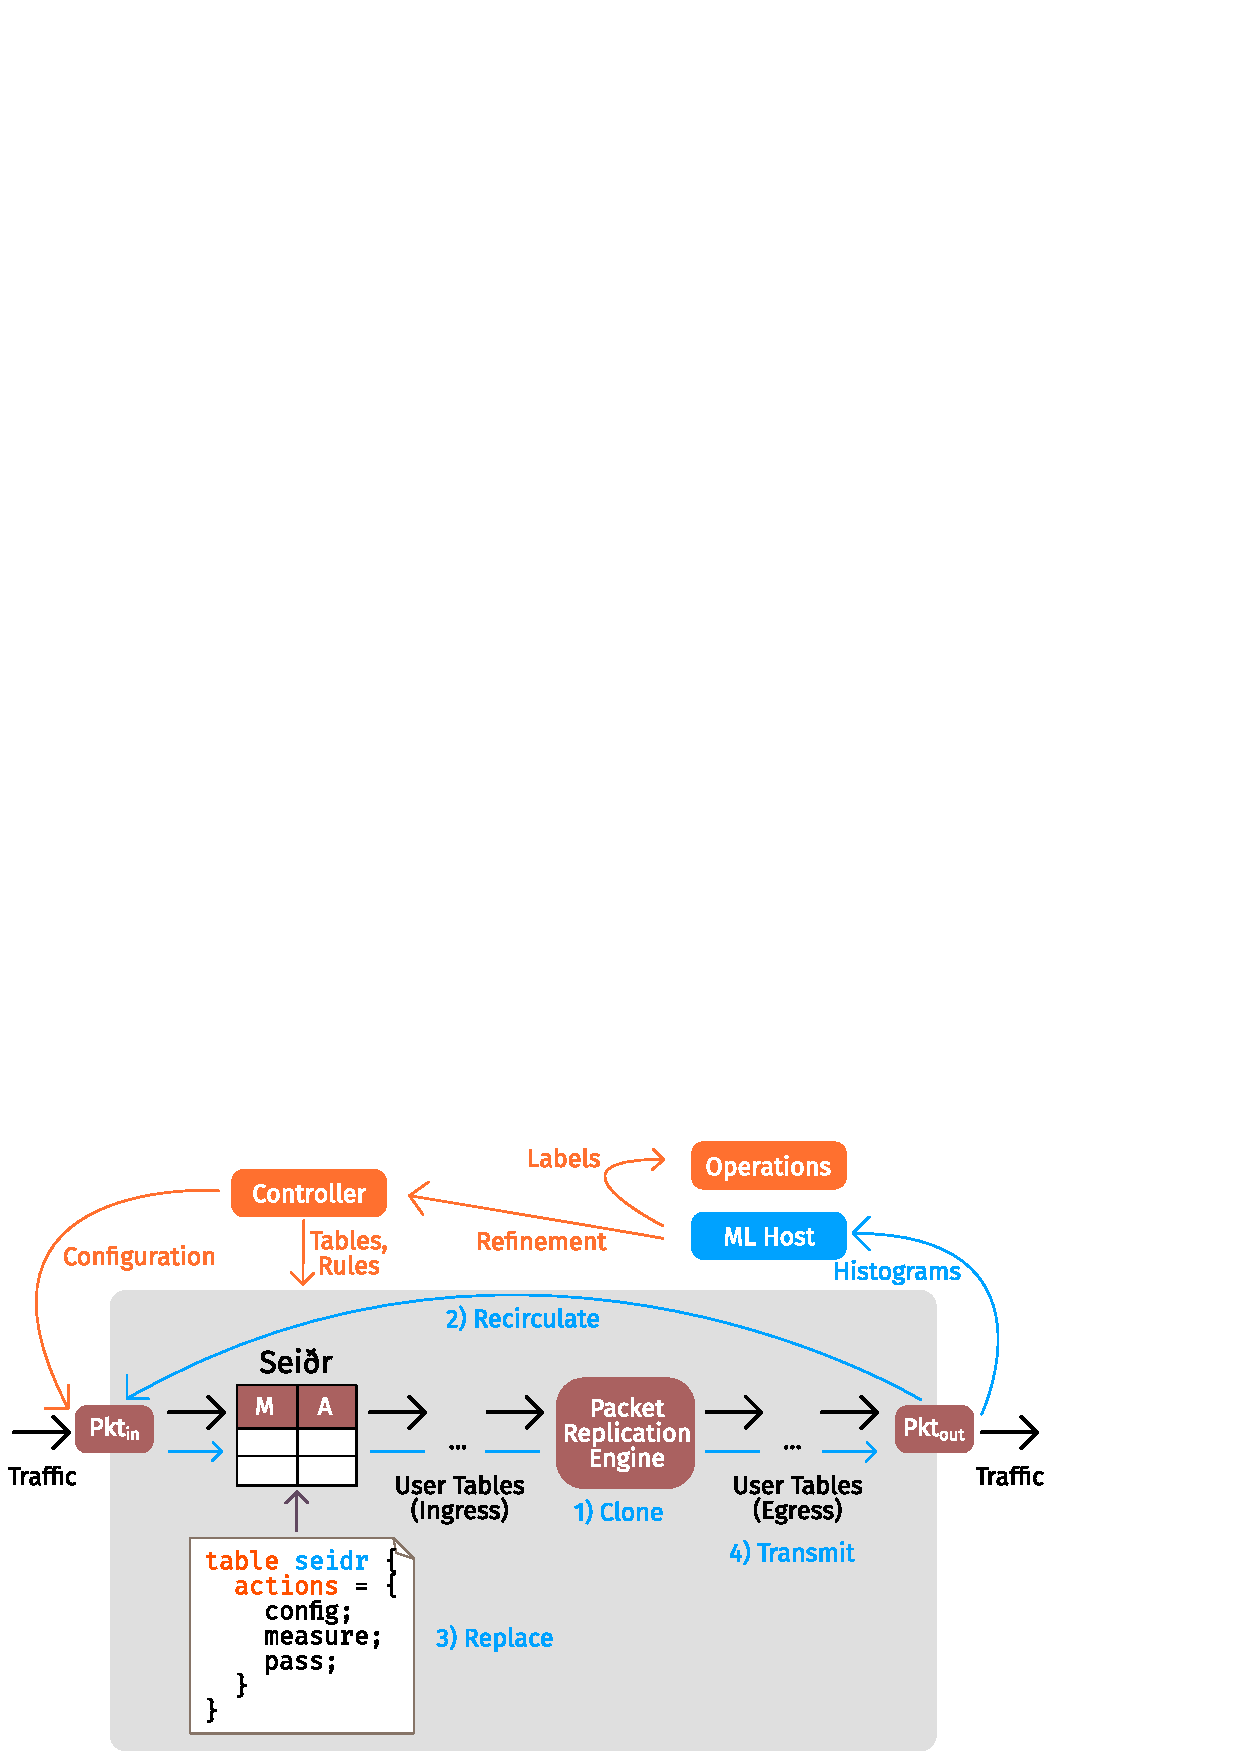
\includegraphics{diagrams/seidr/dp-arch-diagram.pdf}}
    \caption{\seidr{}'s integration with a PSA-compatible~\cite{p4-psa} dataplane.}
    \label{fig:arch}
\end{figure}

% Let's show them a histogram datastructure would look like purely with registers and how would a P4 action populate it - pseudocode or P4 snippet would be nice.

Although packet timing information is useful in understanding network and flow behaviour, without volume or packet rate reduction it is prohibitively expensive for hosts to handle each packet.
Histogramming acts as the \emph{aggregation step} which makes this class of analysis feasible in high-speed networks.
\Cref{fig:arch} demonstrates how \seidr{}, installed as an additional table in any P4 program, records and transmits inter-arrival time histograms.
The format for these histogram packets is outlined in \cref{fig:seidr-headers}; we choose to store individual buckets as \mintinline{rust}{u16}s, and the number of buckets in any histogram is fixed at compile time.
We set this to \num{100} buckets per histogram.
Packets traverse a table which requires \num{3} actions to be implemented:
\begin{enumerate}
    \item \mintinline{rust}{config} reads any matched packets as a \mintinline{rust}{seidr_cfg_t} of type \mintinline{rust}{SET_}\{ \mintinline{rust}{MIN}, \mintinline{rust}{MAX}, \mintinline{rust}{DST}, \mintinline{rust}{SRC}, \mintinline{rust}{LEN} \} by using the P4 parser.
    These update registers \numrange{1}{5} in \cref{tab:registers}, dropping any matched packets.
    
    \item \mintinline{rust}{measure} calculates the inter-arrival time, update per-flow histograms, and transmits finished histograms to the correct host. We describe its operation in \cref{alg:measure}.
    
    \item \mintinline{rust}{pass} ignores packets, and is the default action.
\end{enumerate}
Constructing \seidr{} in this manner allows the control plane to install rules to enable/disable runtime reconfiguration as needed, and to monitor as many or as few flows as desired (\ie, using wildcard rules, or exact matching).

The PSA does not have any mechanisms for generating new packets.
To circumvent this, any packet which would complete a histogram is tagged for cloning at the end of the ingress pipeline, and recirculation at egress (\cref{algline:recirc}).
This truncated copy returns to \seidr{}'s table, where we enable the relevant headers, change L2/3 fields, and write out the histogram contents (\crefrange{algline:rewrite-start}{algline:rewrite-end}).
The P4 deparser outputs the new protocol stack at egress, and transmits the histogram UDP packet into the network.
Event-driven architecture proposals~\cite{DBLP:conf/hotnets/IbanezABM19} may allow a more natural means of packet generation.

\begin{figure}
\centering
\begin{subfigure}{0.45\linewidth}
\centering
\adjustbox{max width = 0.6\linewidth}{
\begin{minipage}{\linewidth}
\begin{minted}[escapeinside=||]{rust}
|\textbf{\textcolor{Keyword}{header}}| seidr_cfg_t {
    bit<8> function;
    bit<144> payload;
}
\end{minted}
\end{minipage}
}
\end{subfigure}
\begin{subfigure}{0.45\linewidth}
\centering
\adjustbox{max width = 0.6\linewidth}{
\begin{minipage}{\linewidth}
\begin{minted}[escapeinside=||]{rust}
|\textbf{\textcolor{Keyword}{header}}| seidr_t {
    bit<128> src_ip;
    bit<128> dst_ip;
    bit<16> src_port;
    bit<16> dst_port;
    bit<16> eth_type;
    bit<BUCKETS * 16> histo;
}
\end{minted}
\end{minipage}
}
\end{subfigure}
\caption{P4 headers for \seidr{} configuration and histograms.}\label{fig:seidr-headers}
\end{figure}

\begin{algorithm}
% \vspace{-0.25cm}
% \DontPrintSemicolon
\KwData{5-tuple, P4 metadata, P4 headers, Registers}
h $\leftarrow$ hash(5-tuple)\;
index $\leftarrow$ BUCKETS * h\;
owner $\leftarrow$ HistoOwner[h]\;
\uIf{metadata.packet\_path = RECIRCULATE}{
    headers.tcp.valid $\leftarrow$ false\label{algline:rewrite-start}\;
    headers.udp.valid $\leftarrow$ true\;
    headers.seidr.valid $\leftarrow$ true\;
    copy 5-tuple into headers.seidr\;
    rewrite headers.ip, headers.udp using HistoSrc/Dest\;
    headers.seidr.histo $\leftarrow$ HistoData[index..]\;
    truncate payload\;
    zero out registers: BucketCount, HistoOwner[h], HistoData[index..]\;\label{algline:rewrite-end}
}
\ElseIf{owner = 0 \textbf{or} owner = 5-tuple}{\label{algline:owner-check}
    HistoOwner[h] $\leftarrow$ 5-tuple\;
    iat $\leftarrow$ LastTimestamp - metadata.mac\_ingress\_time\;
    \If{iat $\ge$ Min \textbf{and} iat $\le$ Max}{
        bucket $\leftarrow$ BUCKETS * (iat - Min) / (Max - Min)\;
        HistoData[index + bucket] $\leftarrow$ HistoData[index + bucket] + 1\;
        BucketCount[h] $\leftarrow$ BucketCount[h] + 1\;
        \If{BucketCount[h] = Len}{
            mark packet for cloning and recirculation\label{algline:recirc}\;
        }
    }
}

\caption{Histogram update and transmission.}\label{alg:measure}
\end{algorithm}

In the event of hash collision (\cref{algline:owner-check}), we ignore packets outside of the tracked flow to ensure that data is accurate.
As later processing and classification directly affect what decisions are made by operators or automatically taken by a policy (possibly leading to incorrect flow limits, QoS, \emph{etc.}), avoiding corruption/cross-contamination of operational data is paramount.
To gain collision resistance, Robin Hood hashing could be used up to a maximum distance in the table, treating a zeroed owner as empty and an illegal source IP as a tombstone value.

\begin{table}
    \centering
    \caption{Register map (Datatype, Amount) for an $h$-bit hash.}
    \resizebox{\linewidth}{!}{\begin{tabular}{@{}ccccccccc@{}}\toprule
        Min & Max & Length & HistoSrc & HistoDest & BucketCount & LastTimestamp & HistoOwner & HistoData \\ \midrule
        \mintinline{rust}{u16} & \mintinline{rust}{u16} & \mintinline{rust}{u16} & \mintinline{rust}{u16 + u128} & \mintinline{rust}{u16 + u128} & \mintinline{rust}{u16} & \mintinline{rust}{u64} & \mintinline{rust}{3 * u16 + 2 * u128} & \mintinline{rust}{BUCKETS * u16} \\
        1 & 1 & 1 & 1 & 1 & $2^h$ & $2^h$ & $2^h$ & $2^h$ \\ \bottomrule
    \end{tabular}}
    \label{tab:registers}
\end{table}

% Basic Logic:
% \begin{itemize}
%     \item table 1: three actions
%     \begin{itemize}
%         \item config: set R1 or R2 (controller installs rule matching a specific port/ip combo)
%         \item measure: take ingress timestamp from metadata, do stuff, write into lasttime, add to bucket and total if within bounds
%         \item pass (default)
%     \end{itemize}
%     \item then pass onto rest of tables
%     \item Why do it this way? can make it all or nothing through control plane.
%     \item How to write and send packet? Same trick as ESNET? (recirc w/ custom metadata to transform pkt)
% \end{itemize}

% ?? NOTE: See PSA \cite{p4-psa} for register format. Some papers, like Dapper, suggest that hash tables should be possible? That would work out very well in our benefit.

% ?? What is configurable? Min, max of the histogramming range

This design allows runtime configuration of all aspects save for the bucket count; at runtime, the only way to increase bucket resolution is to examine a smaller region of IATs.
While in theory this could be configured below a maximum compiled into the firmware, the difficulties introduced in classification/data processing make this infeasible.
Unless using stream-capable classifiers such as LSTMs~\cite{DBLP:journals/neco/HochreiterS97}, changing the input size requires retraining from scratch since new neuron weights must be added and structural properties of the input data change.
Increasing the bucket count requires new firmware installation, as many dataplane P4 implementations cannot allocate variable-length stores due to the lack of a dynamic allocator.

\begin{figure}[t]
    \centering
    \begin{subfigure}[t]{0.49\linewidth}
        \centering
        \resizebox{\linewidth}{!}{\includegraphics{plots/seidr/dt-cubic-1000-app.pdf}}
        \subcaption{TCP Cubic}
        \label{fig:cubic-hist-app}
    \end{subfigure}
    \begin{subfigure}[t]{0.49\linewidth}
        \centering
        \resizebox{\linewidth}{!}{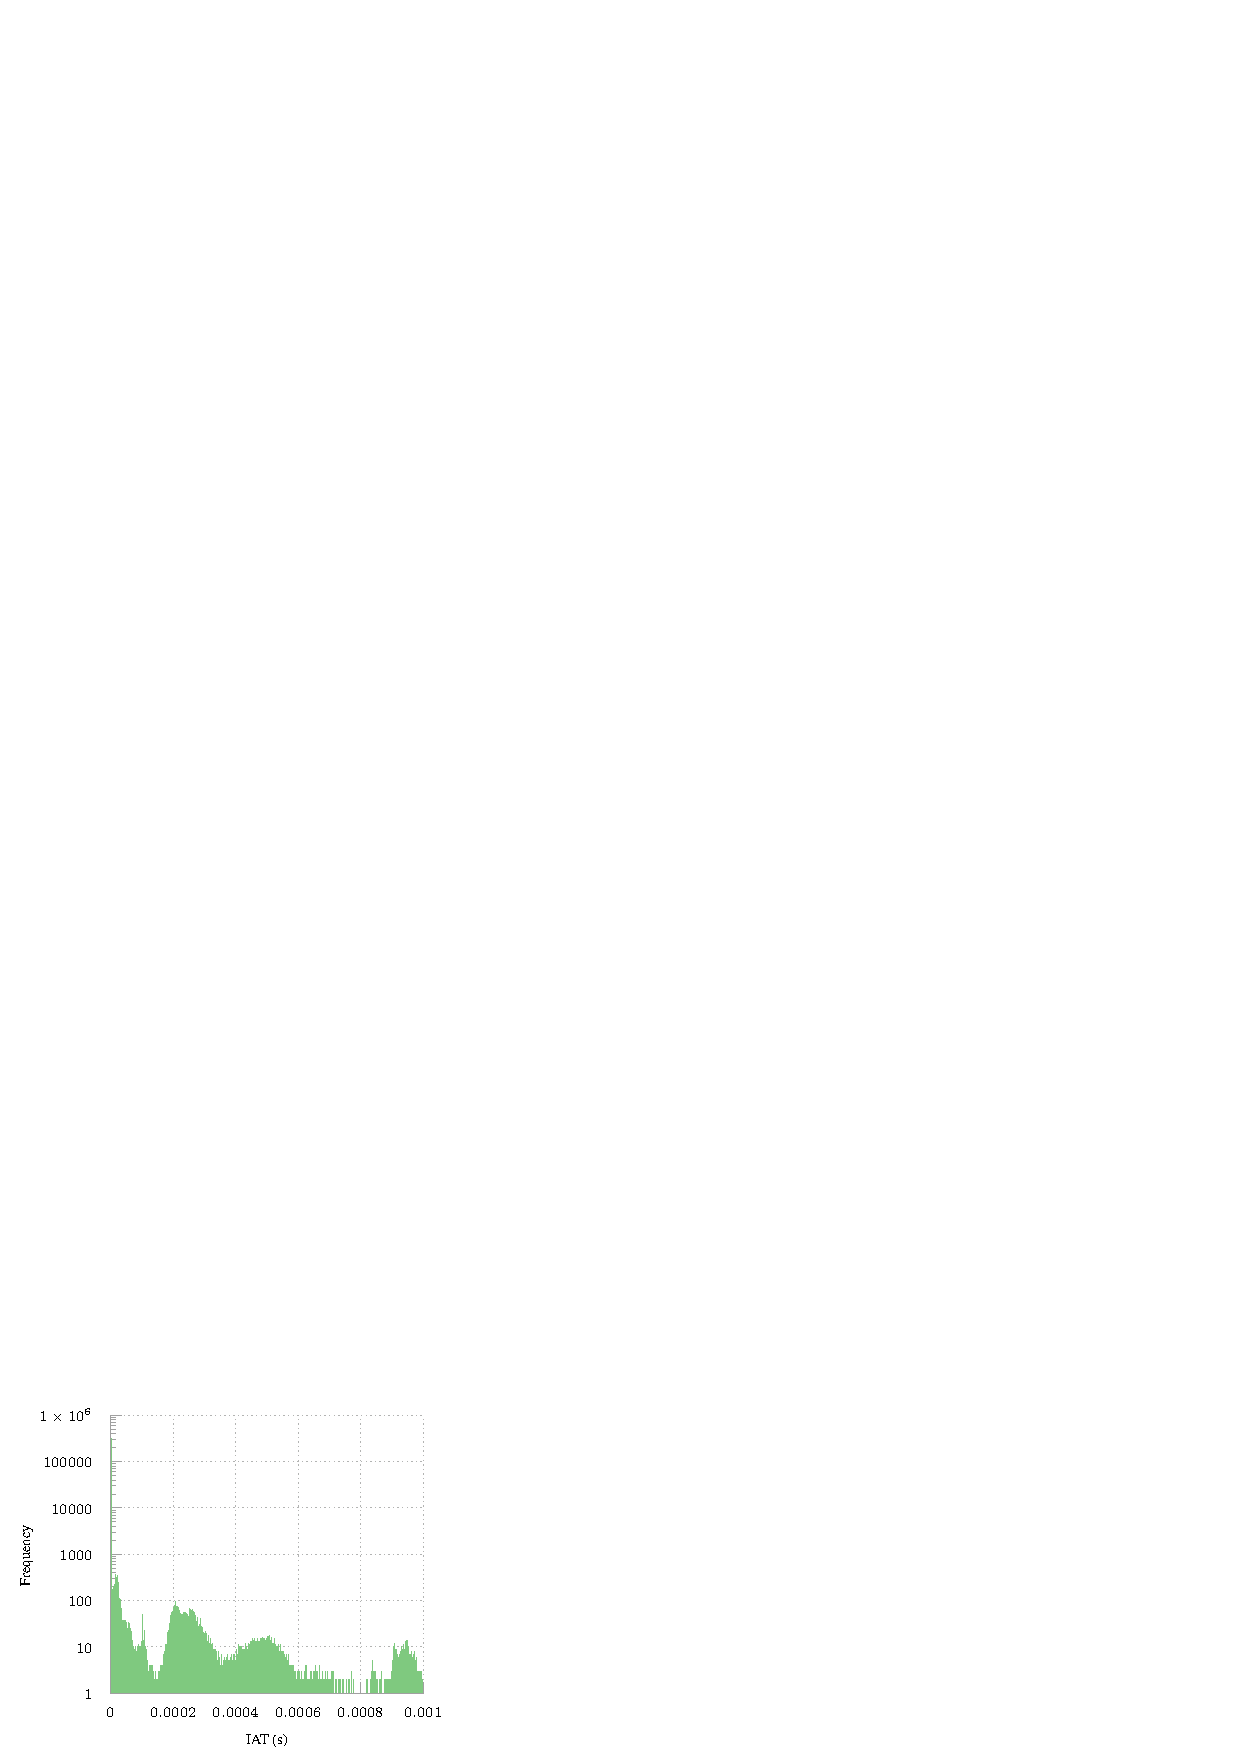
\includegraphics{plots/seidr/dt-bbr-1000-app.pdf}}
        \subcaption{TCP BBR}
        \label{fig:bbr-hist-app}
    \end{subfigure}
    \caption{Example dataplane histograms showing visible differences in inter-arrival times of selected TCP flavours. Our ML solutions are trained to programmatically identify such differences.}
    \label{fig:tcp-hist-app}
\end{figure}

As an example of dataplane-generated histograms, \cref{fig:tcp-hist-app} shows the distribution of inter-arrival times between two TCP congestion control algorithms. The visible differences are programmatically identified using our ML algorithms.

\subsection{Accurate, Precise and High-Resolution Timestamping}

Precise timestamps are critical when detecting temporal properties of flow behaviour, such as microbursts or inferring flow congestion control algorithms.
It is especially important in high speed (\SI{100}{\giga\bit\per\second}) networks, where there can be as little as \SI{6.7}{\nano\second} between packets that need to be analysed.
With a Linux-based software solution (\eg, reading packets from a link with \emph{tcpdump}), the Linux kernel can only provide microsecond-level accuracy with precision in the order of \SI{100}{\micro\second}~\cite{kundel2020p4sta}.
DPDK improves on this, increasing the accuracy to \SI{100}{\nano\second} in the best case~\cite{primorac2017measure}.
However, today's dataplane devices (\eg, Netronome SmartNICs, NetFPGA SUME) allow nanosecond-accurate timestamps to be retrieved from the \emph{Media Access Control} (MAC) modules with a precision of \SI{10}{\nano\second}~\cite{kundel2020p4sta}, a timestamp property \seidr{} relies upon.

% Some platforms provide picosecond-level precision and many solutions allow time synchronisation between multiple devices using the IEEE 1588-2002 (Precision Time Protocol) standard.



\section{TCP congestion control classification}\label{sec:seidr-tcpcc}


% We present an example of first-stage analysis performed for each flow and each packet---stateful TCP analysis.
% This includes numerous metrics which are considered standard when measured at connection endpoints, yet are difficult or invite numerous issues when performed in the network (of which we include a discussion on drawbacks and, curiously, benefits).
% The introduction of accurate timestamps allows us to explore rate-monitoring at a per-packet level, a new view of flow behaviour which may enable flow and hardware characterisation.

% \subsection{Per-Packet Rate Monitoring}

% \begin{figure*}
%     \centering
%     \begin{subfigure}[t]{0.49\linewidth}
%         \centering
%         \resizebox{0.5\linewidth}{!}{
% 	    \begin{tikzpicture}
%     		[packet/.style={draw, fill=uofgsunshine}]
% 		    \node[packet] (p1) {$p_1$: 1500B};
% 		    \node[packet, right= 1cm of p1] (p2) {$p_2$: 800B};
		
% 		    \node at ($(p1.south west) - (0,1)$) (t1) {$t_1$};
% 		    \node at ($(p2.south west) - (0,1)$) (t2) {$t_2$};
		
% 		    \draw[-, dotted] (t1.north)--(p1.south west);
% 		    \draw[-, dotted] (t2.north)--(p2.south west);
		
%     		\draw[<->] (t1.north) -- node[below]{$\mathit{dt}$} (t2.north);
% 	    	\draw[<->] ($(t1.north) + (0,0.2)$) -- node[above]{$s$} ($(t1.north) + (1.8,0.2)$);
% 		    \draw[<->] ($(t1.north) + (1.8,0.2)$) -- node[above]{$g$} ($(t2.north) + (0,0.2)$);
% 	    \end{tikzpicture} 
% 	}
%     \caption{\centering Per-packet rate, visualised. Note that $p_1$ and $p_2$ are not necessarily packets from the same flow.}
%     \label{fig:per-packet-rate}
%     \end{subfigure}
%     \begin{subfigure}[t]{0.49\linewidth}
%     \centering
%     \resizebox{0.9\linewidth}{!}{
% 		\begin{tikzpicture}
% 		[packet/.style={draw, fill=uofgsunshine}]
% 		\node[packet] (p1) {$p_1$: 1500B};
% 		\node[packet, right= 1cm of p1] (p2) {$p_2$: 800B};
% 		\node[right= 1cm of p2] (p3) {...};
% 		\node[packet, right= 1cm of p3] (p4) {$p_{n-1}$: 1500B};
% 		\node[packet, right= 1cm of p4] (p5) {$p_n$: 1500B};
		
% 		\node at ($(p1.south west) - (0,1)$) (t1) {$t_1$};
% 		\node at ($(p2.south west) - (0,1)$) (t2) {$t_2$};
% 		\node at ($(p4.south west) - (0,1)$) (t4) {$t_{n-1}$};
% 		\node at ($(p5.south west) - (0,1)$) (t5) {$t_{n}$};
		
% 		\draw[-, dotted] (t1.north)--(p1.south west);
% 		\draw[-, dotted] (t2.north)--(p2.south west);
% 		\draw[-, dotted] (t4.north)--(p4.south west);
% 		\draw[-, dotted] (t5.north)--(p5.south west);

%         \draw[<->] ($(t2.south) + (0,-0.25)$) -- node[above]{$s$} ($(t2.south) + (6.25,-0.25)$);
%         \draw[<->] ($(t2.south) + (6.25,-0.25)$) -- node[above]{$g$} ($(t5.south) + (0,-0.25)$);
% 		\draw[-, thick] ($(t2.south) - (0,0.5)$) -- node[below]{$W$} ($(t5.south) - (0,0.5)$);
% 		\end{tikzpicture} 
% 	}
%     \caption{\centering Sliding window rate, visualised. Rate estimates are computed using the sizes of the last $W$ packets seen in the current flow. Packets $p_2$ and $p_{n-1}$ belong to the same flow, but $p_n$ is not assumed to.}
%     \label{fig:sliding-window-rate}
%     \end{subfigure}
%     \caption{Comparison of per-packet and sliding window rates. The lengths of packets and inter-packet gaps are not to scale, and are purely demonstrative.}
%     \label{fig:pr-vs-slide}
% \end{figure*}

% Associating each packet with a high-resolution timestamp allows us to introduce the notion of a \emph{per-packet rate}.
% Assuming a packet with size $p$ arrives at time $t_1$ and is followed by another packet (potentially from another flow) which arrives at $t_2$, we measure $\mathit{dt}=t_2-t_1$ for this packet.
% Supposing this first packet spends time $s$ on the wire and assuming that the inter-packet gap $g$ is negligible compared to the length of a packet, then $\mathit{s} = \mathit{dt} - g \approx \mathit{dt}$.
% This packet then has a point rate, $r$:
% \begin{equation}
%     r = \frac{p}{s} \approx \frac{p}{\mathit{dt}}
% \end{equation}
% \Cref{fig:pr-vs-slide} demonstrates how this timing information arises, contrasted with sliding-window rate measurements taken over a longer time period.
% This assumes almost back-to-back traffic, which is realistic in our deployment environment, but to the best of our knowledge no programmable switches expose the timestamp at which the final bit of a packet has been ingested.
% Such a timestamp would allow exact measurement of $s$.

% % ?? we need to be clear about the unintuitive nature of these measurements, include a quick sketch proof which shows that the weighted average of a set of point rates is analytically identical to the sliding window rate/throughput taken over the same period of time.
% While this is an interesting measure to associate with each packet, considering how best to view such rates in aggregate can be counter-intuitive.
% Viewing these rates as time series data reveals interesting distributional characteristics which disagree starkly with our understanding of a flow's rate---for instance, clusters which suggest a different mean.
% Suppose we have a set of measurement indices $C$ with no gaps captured between $t$ and $t'$, partitioned into flows $C = F_1 \cup \dots \cup F_p$.
% To correctly combine a set of point measurements for a flow $F_i$ into an average rate $\overline{r}_{F_i}$, we compute:
% \begin{equation}
%     \overline{r}_{F_i} = \frac{\sum_{a \in F_i} \mathit{dt}_a r_a}{\sum_{c \in C} \mathit{dt}_c}.
% \end{equation}
% In the instance that only one flow is captured (\emph{i.e.}, $F_i = C$), this is a weighted average over point rates, using the $\mathit{dt}$ measured between each packet and the next packet in the same flow as its weight.
% Similarly, this is analytically equivalent to the sliding-window rate measured over the same set of packets:
% \begin{equation}
%     \frac{\sum_{a \in F_i} \mathit{dt}_a r_a}{\sum_{a \in F_i} \mathit{dt}_a} \simeq \frac{\sum_{a \in F_i} p_a}{t' - t}.
% \end{equation}
% % \begin{proof}
% % Given a set of contiguous measurements from the same flow $S \subseteq \mathbb{Z}$, admitting $p_s$, $r_s$, $\mathit{IAT}_s$ and $t_s$, the weighted average of point rates is then
% % $$
% % \overline{r}_S = \frac{\sum_{s \in S} \mathit{IAT}_s r_s}{\sum_{s \in S} \mathit{IAT}_s}
% % $$
% % The sliding-window average:
% % $$
% % \overline{r}_S = \frac{\sum_{s \in S} \mathit{IAT}_s r_s}{\sum_{s \in S} \mathit{IAT}_s}
% % $$
% % \end{proof}

% We assume that inter-packet gaps will be negligible (\emph{i.e.}, that the link is never in a state of very low utilisation), due to typically high utilisation on a WAN.
% % Similarly, we need to discuss the effects of selective monitoring or an abundance of UDP/ICMP traffic (which will distort $dt$s).
% However, this assumption can be distorted if selective TCP flow monitoring is used, or if UDP/ICMP traffic is overabundant; both these scenarios create larger gaps between TCP packets of interest, inflating $g$ to the point where it is comparable in size to $s$.
% This has an impact on our notion of per-packet rates, but not inter-arrival times or other such dependent metrics.
% The effect is small on sliding window rates, particularly at larger window sizes.
% ?? Justify. On paper, it looked like error term was O(1/n), O(g) for an n packet window.


% \section{Inter-Arrival Time}

% Having assigned each packet in a flow with a nanosecond-accurate timestamp ?? tbc

\Cref{fig:tcp-hist-app} suggests that a notable use-case for this type of measurement is \emph{congestion control algorithm} (CCA) detection.
In a TCP connection, each machine is free to choose the CCA it uses to send bytes, and thus how it responds to network congestion signals.
This choice is local, and so is invisible to the other machine (and the network).
In datacentre networks, operators choose these to ensure optimal behaviour.
In a transit network or large WAN however, these hosts (and thus the CCAs in use) are outside the control of network operators, which introduces difficulties when CCA interactions lead to \emph{unfairness}.
Consider the recent (and widespread) introduction of \emph{TCP BBR}~\parencite{DBLP:journals/queue/CardwellCGYJ16}.
\emph{BBR} is a delay/model-based CCA which converges on a fair share of bottleneck bandwidth by reducing its rate if the round-trip time increases, while periodically attempting to increase send rate to account for path/load changes.
However, \emph{BBR} traffic can consume \SI{40}{\percent} of link capacity when multiplexed with loss-based CCAs, regardless of the number of competing flows~\parencite{DBLP:conf/imc/WareMSS19}. 
When ensuring fair transit to all flows, this is hardly a desirable outcome; in fact, it's one which may frustrate clients or violate SLAs.

A curious property of \emph{BBR}'s algorithm which sets it apart from other variants is that packet transmission is \emph{timer-based}.
\texttt{send(packet)}, as defined in the canonical algorithm, asks that on transmission of a packet, the sender should wait for the estimated time that packet would take to reach the recipient.
For instance, at an estimated bottleneck bandwidth of \SI{8}{\mega\bit\per\second}, a \SI{1024}{\kilo\byte} packet would hold back the next packet in the flow until \SI{976.6}{\micro\second} had elapsed.
When packet sizes remain similar this causes strongly periodic behaviour, while mode switches in the \emph{BBR} algorithm cause these periodic bands to shift up or down accordingly.
This effect is stronger than in existing loss- and delay-based algorithms which remain intrinsically tied to the notion of a congestion window (where release of buffered packets follows the receipt of ACK messages).
As a result, timing behaviour of past CCAs may be influenced by (the lack of) packet pacing, periodic components might be made noisier by jitter along the return path, or the behaviour of the receiver might add further noise.

This high-level analysis of \emph{BBR} gives us a strong feature to use as the basis for classification: the \emph{inter-arrival times} (IATs) for each packet in a flow.
We have two options for processing this for classification: we may use a compressed, fixed-size representation such as histograms to capture the aggregate distribution, or we may attempt to capture structural behaviour by using a variable-length stream of IATs.
In many networks, the data and packet rate reduction offered by the former is required to make this possible.
Indeed, in-switch aggregation has seen great success in aiding ML for training~\parencite{DBLP:conf/isca/LiLYCSH19}, and direct execution~\parencite{DBLP:conf/hotnets/XiongZ19}.
We make use of the following standard classification algorithms on a fixed-size representation to attempt to single out the CCA in use:

\begin{itemize}
    \item \emph{$k$-Nearest Neighbours ($k$-NN)}. A simple and well-understood classifier which assigns labels based on the closest members of the training corpus (\ie, by the $L_2$ metric). Linear memory cost in amount of training data, and no training cost other than loading all data points, but capable of learning complex decision boundaries on fixed-length input.
    
    \item \emph{Convolutional Neural Networks (CNNs)}. A neural network approach which learns convolution kernels to classify fixed-length data, particularly when recognising spatial features. Memory cost is fixed for a given architecture irrespective of training data, with a high training cost.
\end{itemize}
% \fakepara{Long Short-Term Memory~\parencite{DBLP:journals/neco/HochreiterS97} units (LSTMs)} A class of recurrent neural network used for stream classification, forecasting, and prediction of variable-length data. Memory cost is fixed, with longer training times (and more data required) than similarly sized CNNs.
% Of these, we apply $k$-NN and CNNs to histograms of packet IATs, and LSTMS to raw IAT streams.

When examining $k$-NN classifiers, we measured accuracy across choices of $k \in \left[2, 8\right]$.
We found $k=2$ to be the most effective choice with our input data using the $L_2$ metric.
Our CNN architecture is described in \cref{tab:cnn-arch}, using ReLu activation and $1 \times 1$ stride in convolutional layers unless stated otherwise.
Training occurred over 5 epochs using the Adam optimiser with categorical cross-entropy as a loss metric, and a batch size of \num{64} histograms (\num{8} for full sequences due to the smaller data volume).
For \emph{BBR vs.\ Cubic}, the complete model consists of \num{104898} 32-bit floating-point parameters (\SI{409.76}{\kibi\byte}), while the full classification task adds a further \num{130} parameters (\SI{0.51}{\kibi\byte}).

\begin{table}
    \centering
    \caption{CNN architecture for \num{100}-entry histograms.}
    \resizebox{0.7\linewidth}{!}{\begin{tabular}{@{}cccc@{}}\toprule
        Layer & Nodes/Filters & Filter Size & Output Dimension \\ \midrule
        Conv2D & 32 & $(3 \times 1)$ & $(98 \times 1 \times 32)$ \\
        MaxPool & --- & $(2 \times 1)$ & $(49 \times 1 \times 32)$ \\
        Conv2D & 64 & $(3 \times 1)$ & $(47 \times 1 \times 64)$ \\
        MaxPool & --- & $(2 \times 1)$ & $(23 \times 1 \times 64)$ \\
        Conv2D & 64 & $(3 \times 1)$ & $(21 \times 1 \times 64)$ \\
        Flatten & --- & --- & \num{1344} \\
        Dense & 64 & --- & \num{64} \\
        Dense (Softmax) & $n_\mathit{classes}$ & --- & $n_\mathit{classes}$ \\
        \bottomrule
    \end{tabular}}
    \label{tab:cnn-arch}
\end{table}


\section{Evaluation}\label{sec:seidr-evaluation}
%Traffic is played back from hosts via Tcpreplay at a bandwidth assigned uniformly from a `good' or `bad' distribution, each using the same pcap file with source and destination IP addresses rewritten.

This work is most naturally compared against Marl, introduced by \textcite{DBLP:journals/eaai/MalialisK15}, the state-of-the-art in \gls{acr:rl}-based \gls{acr:ddos} prevention.
We are most interested in seeing how their approach contrasts with the new agent designs across different topologies and workloads.
Different network environments will also impose different levels of host density, where popular web servers may have orders of magnitude more clients than egress points from their network---I aim to show how these characteristics affect performance and learning rate.
Marl is known to outperform the AIMD~\parencite{DBLP:journals/ton/YauLLY05} strategy, yet the state of the art has long since moved on.
To paint a more current picture, I compare this work against an effective modern approach, \emph{SPIFFY}~\parencite{DBLP:conf/ndss/KangGS16}.
SPIFFY tests a proportion of flows by routing them through an alternate path with higher bandwidth, observing how their speed changes some time later.
This comparison lets us position our new agent designs against the state of the art, observing that SPIFFY has a similar mode of interaction to \gls{acr:rl}-based systems (taking action, observing an effect, and acting once again) and does not rely on protocol characteristics or signatures.
In reimplementing SPIFFY, I make the simplifying assumption that a suitable unused path exists (with identical bandwidth to the server's link).
\qty{10}{\percent} of active flows were tested at a time (according to the authors' observation that there is a factor of \qty{10}{\times} difference between the ideal and achieved bandwidth expansion), excluding flows below \qty{50}{\kilo\bit\per\second} and requiring a \qty{3}{\times} expansion from legitimate flows, making a judgement after \qty{5}{\second}.

To test this, I made use of both traffic models introduced in \cref{sec:a-new-normal} (Opus and \gls{acr:tcp}), both topologies discussed below (1-dest vs.\ Fat-Tree), and vary the amount of hosts typically communicating over each agent's ingress/egress node.
Additionally, these new models were evaluated in multi-agent mode (\emph{separate}, no model sharing), and in single-agent mode (\emph{single}, zero-cost perfect information sharing).
In each case, the algorithm's performance was averaged over \num{10} episodes of length \num{10000} timesteps (setting each agent's $\wvec{}=\mathbf{0}$ between episodes).
Host allocations at the beginning of each episode were generated pseudorandomly to ensure fairness between episodes---a host is malicious with probability $\operatorname{P}\left(\mathit{malicious}\right)$, and is benign otherwise.
Benign hosts generate traffic according to either \cref{sec:tcp-http-traffic-model,sec:udp-opus-traffic-model} depending on the experiment, while malicious hosts generate traffic as described in \cref{sec:attack-traffic-model} (both at experiment-dependent rates).

All experiments were executed on Ubuntu 18.04.2 LTS (GNU/Linux 4.4.3-040403-generic x86\_64), using an Intel Core i7-6700K (\qtyproduct[product-units=single]{4 x 4.2}{\giga\hertz}) which had \SI{32}{\gibi\byte} of \gls{acr:ram}.
%All code underpinning these findings is available on a public repository\footnote{\url{https://github.com/FelixMcFelix/rln-dc-ddos-paper}}.
%All code underpinning these findings is available on a public repository.\footnote{Private until publication.}

\subsection{Single destination}\label{sec:single-dest}
%?? Move description of tree topol to here.
The network is tree-structured, where one server $s$ connects through a dedicated switch to $k$ team leader switches, each connected to $\ell$ intermediate switches, which in turn each connect to $m$ egress switches.
We then have $N_{\mathit{hosts}} = k \ell m n$.
\Cref{fig:marl-topol} demonstrates this.
%Although \citeauthor{DBLP:journals/ccr/MahajanBFIPS02a}, the originators of this topology, make it clear that it exists as a fairly unrepresentative example \cite{DBLP:journals/ccr/MahajanBFIPS02a}, it remains the case that such a network topology allows for functional testing, and indeed is illustrative of one way in which attack traffic might aggregate in the network.
%It is hard, however, to argue its relevance to specific classes of victim or to reason about the interactions it might have with dependent applications.
%We aim to address this through \cref{sec:performance-in-an-emulated-environment}.
The network topology was configured using $k=2$ teams, $\ell=3$ intermediate nodes per team, $m=2$ agents per intermediate node, and $n \in \{2, 4, 8, 16\}$ hosts per learner.
This is a slight simplification of \Textcite{DBLP:journals/eaai/MalialisK15}'s \textquote{online} experiment, choosing fewer teams but remaining as a single server with a fan-out network.
%The algorithm parameters were set at $\gamma=0$ (leading to opportunistic behaviour), $\alpha=0.05$, having linearly annealed $\epsilon=0.2 \rightarrow 0$ by $t=3000$.
%Benign and malicious hosts uploaded between \SIrange{0}{1}{\mega\bit\per\second} and \SIrange{2.5}{6}{\mega\bit\per\second} respectively, and hosts were redrawn at each episode's start with $\operatorname{P}(\mathit{malicious})=0.4$.
%$U_s$  $k \ell mn+2$ \si{\mega\bit\per\second}.
%The performance of each choice of $n$ was averaged over \num{10} episodes of length \num{10000} timesteps (setting each agent's $\wvec{}=\bm{0}$ between episodes).
%Host allocations were generated pseudorandomly to ensure fairness between choices of $n$.
%These parameter choices match those of the original study to enable direct comparison, and are (to the best of our knowledge) arbitrary, but we justify our range of $n$ as capturing increasing scales of host activity.

\begin{figure}
	\centering
	\resizebox{0.9\linewidth}{!}{\begin{tikzpicture}[
	texts/.style = {text=black},
	labeltexts/.style = {text=uofgsandstone},
	treeline/.style = {draw=uofgburgundy},
	treenode/.style = {texts, circle, centered, fill=white, treeline},
	load/.style = {fill=uofgcobalt},
	loadhide/.style = {fill=uofgcobalt!40!white},
	external/.style = {fill=uofgrust},
	externalhide/.style = {fill=uofgrust!40!white},
	hideline/.style = {draw=uofgsandstone!40!white},
	hidenode/.style = {treenode, hideline},
	grow'=right
]
	\node[treenode, label={[texts]above:Server}] (root) {}
	child [treeline] { node [treenode, label={[texts]above:Core}] (sswitch) {}
		child [treeline] { node [treenode, label={[texts]above:Leader}] (teaml) {} 
			child [treeline] { node [treenode, label={[texts]above:Intermediate}] (inter) {}
				child [treeline] { node [treenode, load, label={[texts]above:Agent/Egress}] (agent) {}
					child [treeline] { node [treenode, external] (extern) {}
						child [treeline] { node [treenode, external, label={[texts]above:Host}] (host) {} }
						child [hideline] { node [hidenode, externalhide] (endhost) {} }
					}
				}
				child [hideline] { node [hidenode, loadhide] (endagent) {} }
			}
			child [hideline] { node [hidenode] (endinter) {} }
		}
		child [hideline] { node [hidenode] (endteaml) {} }
		edge from parent
		node[below, labeltexts] {$U_s$}
	};
	
	%\draw[-] (teaml) -- (endteaml);
	\node [labeltexts] (kdots) at ($(teaml)!0.5!(endteaml)$) {$\rvdots$};
	\node [labeltexts, right = -0.1cm of kdots] {$k$};
	\node [labeltexts] (ldots) at ($(inter)!0.5!(endinter)$) {$\rvdots$};
	\node [labeltexts, right = -0.1cm of ldots] {$\ell$};
	\node [labeltexts] (mdots) at ($(agent)!0.5!(endagent)$) {$\rvdots$};
	\node [labeltexts, right = -0.1cm of mdots] {$m$};
	\node [labeltexts] (ndots) at ($(host)!0.5!(endhost)$) {$\rvdots$};
	\node [labeltexts, right = -0.1cm of ndots] {$n$};
\end{tikzpicture}}
	\caption[Tree-structured network topology diagram for evaluating a single-destination network.]{
		Network topology diagram, showing how the server and its core switch's $k$ teams are structured, with $\ell$ intermediate routers per team, connected to $m$ agents which each moderate $n$ hosts beyond a single external switch.
		%	Empty nodes are considered to be internal.
		Red nodes are external, and each blue node hosts an agent.
		\label{fig:marl-topol}
	}
\end{figure}

\subsection{Multiple destinations}
The previous topology allows for direct comparison against the state-of-the-art, and indeed is illustrative of one way in which attack traffic might aggregate in the network.
It is hard, however, to argue its relevance to specific classes of victim or to reason about the interactions it might have with dependent applications.
In contrast, the fat-tree topology~\parencite{DBLP:conf/sigcomm/Al-FaresLV08} sees regular use in real-world data centres and scales well horizontally.
%?? Come up with description of fat-tree (multi-dest) topol.
%?? Why fat tree? regularly appears in modern datacentres.
%?? $k=4$ fat-tree , with one pod hosting two servers $s_0,s_1$.
We use a $k=4$ fat-tree, with one pod hosting two servers $s_0$ and $s_1$.
$n$ external hosts connect through each core switch (where agents are hosted), and communicate with $s_0, s_1$ uniformly randomly.
Both servers host identical services.
We set $n \in \{6, 12, 24, 48\}$ hosts per learner (keeping $N_{\mathit{hosts}}$ identical to each tier of the single-host topology), and restrict $U_{s_0} = U_{s_1} = U_s / 2$.

\subsection{Parameters}
The algorithm parameters were set at $\alpha=0.05$, linearly annealing $\epsilon=$ \num{0.2} $\rightarrow$ 0 by $t=$~\num{3000} in the case of Marl (\num{8000} actions per agent in the \emph{Instant/Guarded} models).

Benign hosts each occupied \qtyrange{0}{1}{\mega\bit\per\second}, and hosts were redrawn at each episode's start with $\operatorname{P}(\mathit{malicious})=$~\num{0.4}.
%The original introduction of this approach to direct-control reinforcement learning as introduced by \textcite{DBLP:journals/eaai/MalialisK15} fails to consider key cases: the absence of a suitable heuristic classifier $g(\cdot)$, disjoint ranges of traffic distribution (i.e., the presence of benign heavy-hitters), the accurate simulation of TCP-like behaviour (and its effects on collateral damage), and high densities of hosts at egress points.
%?? Why? ...
%Of these, the latter two are most deserving of a closer investigation, as they have stronger implications for wide-scale deployment.
%These are important issues, particularly when we consider real-world deployment.
%Heuristic estimates of traffic legitimacy come with computational cost and couple the reward function to the accuracy of the estimator, hosts often show diversity in their own traffic patterns (perhaps being multi-modal), and it is known that TCP is the most used transport protocol for Internet traffic \cite{DBLP:conf/saint/ZhangDJC09}.
%?? NEED TO VERIFY VOLUME OF CONGESTION-AWARE PROTOCOLS
Malicious hosts each sent \qtyrange{2.5}{6}{\mega\bit\per\second} when attacking \gls{acr:udp} traffic, though this was increased to \qtyrange{4}{7}{\mega\bit\per\second} when using \gls{acr:tcp}-like traffic (to meaningfully impact benign flows).
Given $n$ and $\operatorname{P}(\mathit{malicious})$, we see an expected malicious bandwidth \numrange{1.27}{1.87} and \qtyrange{2.03}{2.18}{\times} $U_s$ respectively.
%The expected fraction of $U_s$ consumed by each host is \SI{21.5}{\percent} for $n=2$, and \SI{2.84}{\percent} for $n=16$.
For these choices of $n$ in both topologies, we observe $N_{\mathit{hosts}} \in \left\{24, 48, 96, 192\right\}$, and an expected number of malicious hosts $\mathbb{E}\left[N_{\mathit{attackers}}\right] \in \left\{9.6, 19.2, 38.4, 76.8\right\}$.
For the largest choice of $n$, we see an expected total attack traffic $\mathbb{E}\left[V_{\mathit{attack}}\right] =$ \qtylist{334.05;422.4}{\mega\bit\per\second} for Opus and \gls{acr:http} traffic respectively.

$U_s$ was fixed at $N_{\mathit{hosts}}+2$ \unit{\mega\bit\per\second} (to account for burstiness), and each link had a delay of \qty{10}{\milli\second}.
All links had unbounded capacity, save for each server-switch.
These parameters match those of the original study to enable direct comparison, and many are (to the best of our knowledge) arbitrary, but I justify the range of $n$ as capturing increasing scales of host activity.

% \section{Related Work}\label{sec:related}
% %?? Try and compare my work here when possible?

\fakepara{DDoS Prevention}
\Textcite{DBLP:conf/lcn/BragaMP10} examine the detection of flooding DDoS attacks through \emph{self-organising maps}, using SDN to gather statistics effectively.
Many of their features aren't overly relevant, as their focus is not active defence or discovering \emph{which} hosts contribute to an attack.
%?? Actually talk about Marl (???) to appease reviewer \#1.
The closest available approach within this field is that of \textcite{DBLP:journals/eaai/MalialisK15} (whom we have positioned our work against), and their contribution in applying RL to the task of intrusion prevention is significant: their work helps to show the viability of live, adaptive, feedback-loop-like control of the network to detect and prevent DDoS attacks.
They create a tree overlay topology (subdivided into teams), where each agent applies packet drop to \emph{all} flows inbound to a protected server.
%?? Recap their flaws, since they've been cut form every other aspect.
Our results show that their technique underperforms at high host density and when congestion-aware traffic dominates---that their results do not demonstrate this suggests an evaluation driven purely by traces (rather than live application dynamics).

\emph{SPIFFY} \cite{DBLP:conf/ndss/KangGS16} aims to remedy transit-link attacks by observing how flows from each source respond to a sudden increase in available bandwidth.
\Citeauthor{DBLP:conf/ndss/KangGS16} realise that bots participating in an attack are often unable to match this bandwidth expansion (having already saturated the capacity of their outbound links), while legitimate flows typically speed up to match the new fair-share rate.
%Attackers must either be detected or reduce the throughput of each bot, increasing the cost of launching an attack.
%Unlike our approach (and due to the class of attacks it is designed to defend against), SPIFFY is intended to be deployed within ASes, although .
A weakness of their approach is that computing a route to measure bandwidth expansion on real networks can be costly (up to \SI{14}{\second} for the Cogent topology), and that the low expansion factors in real network can require more ``rounds'' of filtering.
By contrast, our approach takes a constant time to compute an action for a flow regardless of topology size.
Their assumptions about traffic response to such bandwidth expansion do not hold for constant bitrate flows (e.g., VoIP) and may not extend to HTTP DASH flows, both of which make up a sizeable proportion of network traffic.

\emph{Athena} \cite{DBLP:conf/dsn/LeeKSPY17} is a generalised SDN framework for intrusion detection, but has shown the use of a \emph{k-nearest neighbours} classifier to detect individual attack flows.
Although heavyweight (and proven to be effective compared with \textcite{DBLP:conf/lcn/BragaMP10}), their comparison against SPIFFY lacks the quantitative evidence required to understand how the system compares.
\Textcite{DBLP:conf/sp/SmithS18} use AS-level routing to tackle both transit-link and flooding-based attacks.
This view is taken due to the perceived cost of per-stream classification and inherent sensitivity to adversarial examples.
The approach is creative, relying upon BGP \emph{fraudulent route reverse poisoning} to preserve traffic to a target AS, but unlike SPIFFY the approach doesn't actually \emph{remove} the congestion.
Because of this, flooding-based attacks aren't fully alleviated.

%?? Abuses of RL 
\fakepara{RL in Networks}
Earnest, well-considered application of RL towards the challenge of intrusion prevention has seen comparatively little examination.
Past work treats the paradigm as a traditional classifier for anomaly detection \cite{shamshirband2014anomaly} and DDoS prevention \cite{DBLP:conf/mates/ServinK08}.
Given that the main strengths of RL techniques are the ability to control ongoing interaction and adapt by observing the concrete effects of actions, such works don't apply the rich literature on the subject to its fullest potential.

For categorising how RL fits into solving problems, we label works as direct- or indirect-control RL.
A \emph{direct-control} RL problem is one where the RL agent(s) learn optimal control over a set of actions as the \emph{primary} defence or decision-maker---requiring measurements, reward functions and action sets tailored for this purpose.
%We feel there is a shortage of work in this category at present, at least in the field of networks.
To date, the best-fitting example we have encountered is that of \textcite{DBLP:journals/eaai/MalialisK15}.
An \emph{indirect-control} RL problem is one where agents act in service to \emph{another technique} responsible for decision-making, optimising or generalising aspects of its operation beyond that of hand-coded heuristics.
A past example includes learning when best to share knowledge between \emph{hidden Markov model} anomaly detectors \cite{DBLP:conf/paisi/XuSH07}.
%The position of this work is weakened by its reliance on the problematic `DARPA99' dataset \cite{DARPA-IDD, DBLP:conf/cisda/TavallaeeBLG09, DBLP:conf/sp/SommerP10}, but the idea itself is well-treated and this acts as a driver for improvements in this direction.
This work is weakened by its reliance on the problematic `DARPA99' dataset \cite{DBLP:conf/sp/SommerP10}, but the idea itself is well-treated.
Outside of intrusion detection, there has been growing interest in the use of RL in data-driven networking, such as for intra-AS route optimisation \cite{DBLP:conf/hotnets/ValadarskySST17} and resource-constrained process allocation \cite{DBLP:conf/hotnets/MaoAMK16}.
\textcite{DBLP:conf/sigcomm/MaoNA17} employ client-side observations of network state and video performance with RL to optimise bitrate selection for multimedia streaming.
\emph{AuTO} \cite{DBLP:conf/sigcomm/ChenL0L18} employs deep RL to perform traffic optimisation.
Crucially, they find that the vast majority of flows are short-lived, requiring effective decisions in less than a millisecond.
To overcome the high latency of action computation via a neural network, two agents are trained, handling aspects of short and long flows respectively.
The first learns to optimise the flow size thresholds to demarcate long and short flows; these short flows are routed by ECMP.
The second agent makes bespoke decisions about routing, prioritisation etc.\ for each of the remaining long flows.


\section{Summary}\label{sec:seidr-conclustion}
We have presented \seidr{}, a dataplane assisted flow classification solution that can be used to detect fine-grained temporal flow behaviour. We have shown a PSA-compliant way to implement in-network data aggregation in the form of histograms, while using nanosecond-precision timestamping. Our in-network generated histogram datastructure (\eg, on per-flow packet inter-arrival times) has been presented as the input for various ML algorithms, including CNN and $k$-NN. We have shown with our extensive evaluation that \seidr{} can successfully tell apart TCP CCAs, in particular, it identifies BBR from its predecessors with over \SIrange{88}{96}{\percent} accuracy, while only consuming a maximum \SI{15.5}{\mebi\byte} of dataplane memory. We presented the trade-offs between training and inference times, memory requirements, and accuracy in the context of CNN and $k$-NN classifiers and shown that \seidr{} outperforms prior work by increasing classification accuracy on novel TCP CCAs, providing the ability to classify at very high traffic rates (in the order of \SI{10}{\tera\bit\per\second}).
Furthermore, we have identified a key temporal property of \emph{BBR} which allows its easy detection among other flows.
In the future, we aim to examine the use of \seidr{} towards microburst detection and diagnosis~\cite{DBLP:conf/sigcomm/ChenFKRR18} and for the identification of \emph{BBR}-like temporal properties of emerging UDP-based congestion-aware protocols, such as \emph{QUIC}.%~\cite{DBLP:conf/sigcomm/LangleyRWVKZYKS17}.

?? Through this chapter, we have discussed ..., lending credence to one of the claims in my thesis statement: \superrecallthesis{3}


% -----

%\part{Improving Deployability}

\chapter{Scalable Flow Classification}\label{chap:seidr}

% \section{Motivation}
% \section{Sei\dh{}r Histograms}
% \subsection{Algorithm}
% \subsection{Packet Generation on PSA}
% \section{Use case: TCP CCA Detection}
% \subsection{Observable Differences}
% \subsection{Investigating the BBR Algorithm}
% \section{Methodology}
% \subsection{Testing Environments}
% \subsection{Data Collection/Generation}
% \subsection{ML Model Architecture}
% \section{Evaluation}
% \subsection{Device Memory Costs}
% \subsection{Bandwidth Costs}
% \subsection{CCA Detection Accuracy and Costs}

?? Problem statement: damn, all this ML is cool
?? We can do cool real-time analysis of operational Internet traffic
?? What do we do if we need more complex ML models: i.e., need to use LSTMs, or complex CNNs because we need to make use of complex temporal or structural features of data? We still need to get it to host machonies.
?? Okay... but in that case, how can we reduce data so that PPS and Gbps of data don't overwhelm the host, or that we lose lots of asid data and make poor decisions when we have many (or very fast) flows?

?? Relate some of this \emph{specifically} back to discussion of flow measurement in the dataplane in the INC use-cases? (i.e., considering all th below IPfix, sFLow, etc. etc.)
?? Try to relate some of the same problems.

There has been significant research and development on real-time analysis of operational Internet traffic.
Accurate flow characterisation (or \emph{classification}) can drive intrusion detection, detecting unusual or illegal patterns of network traffic, or to prioritize traffic for certain customers, to provide path-diversity as well as to mark Quality of Service (QoS) of various users and protocols~\parencite{DBLP:journals/ccr/BernailleTASS06,DBLP:conf/lisa/Roesch99}.
However, flow classification solutions today can usually only rely on sampled data provided by routers, such as sFlow, Netflow, or IPFIX, along with imprecise timing (\si{\micro\second} and \si{\milli\second}-level)~\parencite{rfc7011,rfc3954}.
While sampled, low-precision telemetry can be used to classify network traffic based on some flow properties (such as port and protocol numbers)~\parencite{DBLP:conf/iwcmc/RossiV10}, it cannot be used to classify based on fine temporal properties (\eg, identifying bursty flows and senders that can cause microbursts and buffer overflow on the network).

On the other hand, full-software solutions for traffic classification have been proposed by commercial vendors (\eg, Barracuda DPI\footnote{https://www.barracuda.com/glossary/deep-packet-inspection}), the open-source community (\eg, Snort~\parencite{DBLP:conf/lisa/Roesch99}, Zeek (formerly Bro)~\parencite{DBLP:conf/uss/Paxson98,zeek}), and the research community, with extensible feature sets and algorithms for classification~\parencite{DBLP:conf/icccn/HagosEYK18}.
Unfortunately, these software solutions designed for commodity hardware do not provide accurate timing of packets, and therefore make certain time-critical events hard or impossible to detect (\eg, microbursts~\parencite{DBLP:conf/sigcomm/ChenFKRR18} or congestion control properties~\parencite{DBLP:conf/icccn/HagosEYK18}).
Moreover, even the most sophisticated software solutions process packets orders of magnitude slower than current backbone traffic of large operators, making them unusable for large-scale operational analysis~\parencite{DBLP:journals/wpc/ParkA17}.

At the same time, programming and fast reconfiguration of network devices is being explored in all types of networks: datacenter and cloud networks, CDNs and WANs.
Specifically, with the recent developments of generalized dataplanes (\eg, the \emph{Portable Switch Architecture}~\parencite{p4-psa}), target devices (\eg, Barefoot Tofino and Netronome SmartNICs) along with the high-level programming languages presented for them (\eg, P4~\parencite{DBLP:journals/ccr/BosshartDGIMRSTVVW14}), operators can now express in-network functionality running on their devices, including accurate nanosecond-precision packet timing.
However, programming in-network services has its own challenges (\eg, restricted instruction sets, data types and memory), prohibiting the implementation of a fully in-network classification solution.

% To solve the aforementioned challenges, this paper presents an architecture that marries the precision timing and fast data aggregation capabilities of the dataplane with software classifiers that can run complex classification models due on a the reduced data rate.

To solve the aforementioned challenges, we present \seidr{}\sidenote{Pronounced ``SAY-ther''. ?? Explain naming?}, a dataplane assisted flow classification solution.
Our design philosophy of \seidr{} keeps functionality where it belongs: dataplane devices create accurately timestamped, aggregated data structures for our analysis, and we let a scalable software stack perform ML-based classification on commodity machines.\sidenote{?? Yeah this directly contradicts the main theme and line of reasoning of my thesis LMAO}
As in-network aggregation reduces the data rate by a factor of $\sim$\num{740}, our solution can analyse aggregated data from a total rate of \SI{10}{\tera\bit\per\second} original traffic using a single commodity processing machine.

As a concrete use-case, we look at fine dynamics of TCP congestion control algorithms.
Understanding and classifying them is important for network providers as inadequate choices have severe effects on transfer rates, especially in networks with high bandwidth-delay product~\parencite{DBLP:journals/queue/CardwellCGYJ16} and in networks where multiple congestion control algorithms are used~\parencite{DBLP:conf/imc/WareMSS19}. 
By using accurate congestion control diagnostics, operators will be able to infer sender problems (\eg, backlogged or application-limited senders), network inefficiencies (\eg, increased path latency and congestion), as well as receiver issues (\eg, delayed acknowledgements, small receiver windows) and fairness issues between delay-based and loss-based algorithms~\parencite{DBLP:conf/imc/WareMSS19}.

The contributions of this paper are summarized below:
\begin{itemize}
	\item A flexible dataplane-assisted architecture compatible with the \emph{Portable Switch Architecture} (PSA)~\parencite{p4-psa} that allows data aggregation in the form of histograms with nanosecond-accurate timing (\Cref{sec:architecture}),
	\item A high-accuracy method for telling apart timer-based (\eg, BBR) and cwnd-based TCP flavours using our system with machine learning algorithms (\Cref{sec:tcpcc}),
	\item An extensive evaluation of TCP congestion control classification using our solution (\Cref{sec:evaluation}).
\end{itemize}

The work presented in this chapter considers how \gls{acr:pdp} hardware can reduce input, though fine-grained, measurements into digests suitable for \gls{acr:ml} models running on host machines, and is based upon \citetitle{DBLP:conf/globecom/SimpsonCP20}~\parencite{DBLP:conf/globecom/SimpsonCP20}.
?? Then summarise contents from here...

?? Big open qs:
?? relevance of PSA digests? These can emit packets, no? These can emit an arbitrary struct to the ctl plane over P4Runtime API. Might be good if no digest support, . Digests have a few extra benefits: In some dataplanes can be emitted in egress. Is message fusion a possible downside? (unpredictable)
?? Maybe 2 options? Can be in-band or out-of-band. Digests are the out-of-band option, meanwhile in-band allows you to use dataplane to forward to accelerators like BrainWave (don't add extra load to ctl plane in this way?)

?? Header size limits are the other main constraint.
?? THis is probably not a problem with digests.
?? WHen emitting to dataplane, however? Will have plat-dependent limits on output. Header size limits, PHV limits, register access reqs that could prevent digest access? Need to mark in-progress histo emissions, progress for each, and emit bitslices spread over multiple egress pkts. Logic: CLONE LOOP WHile still pkts to write, block updates to histo if progress (1 bit?). Limitation: Histo emission freq must be reduced to prevent massive traffic amp. slicing logic could be extended to include the digest case? Are there PHV limits in the digest case that make this really suck?

%\section{Introduction}\label{sec:seidr-introduction}
%Network anomaly detection and intrusion detection/prevention are continually evolving problems, compounded by the partial, non-\emph{independent and identically distributed} (IID) view of data at each point in the network.
Attacks and anomalous behaviours evolve, becoming more sophisticated or employing new vectors to harm a network or system's confidentiality, integrity, and availability without being detected \cite{DBLP:journals/comsur/BhuyanBK14}.
These attacks and anomalies have measurable consequences and symptoms which allow a skilled analyst to infer new signatures for detection by misuse-based classifiers, but unseen attacks may only be defended against after-the-fact.
This issue is inherent to \emph{misuse-} or \emph{signature-based} intrusion detectors, and it has been long-hoped that \emph{anomaly-based} detectors would surpass this by making effective use of statistical measures \cite{DBLP:journals/comsur/BhuyanBK14}.

While \emph{machine learning} (ML) approaches seem like a sensible fit for this problem, in \citeyear{DBLP:conf/sp/SommerP10} \citeauthor{DBLP:conf/sp/SommerP10} identified the `failure to launch' of ML-based anomaly detection systems---a distinct lack of real-world system deployments \cite{DBLP:conf/sp/SommerP10}.
To quite a large extent, this remains the case today.
They posit that their use is made difficult due to significant operational differences from standard ML tasks, including: the high cost of errors and extraordinarily low tolerance for false positives inherent to network intrusion detection \cite{DBLP:conf/ccs/Axelsson99}; a general lack of recent, openly available (and high-quality) training data; and diversity of network traffic across varying timescales combined with significant burstiness \cite{DBLP:journals/ccr/LelandWTW95}.
Above the aggregate level, the constant deployment of new services and protocols means that traffic is \emph{non-stationary} and displays an evolving notion of normality.
Learning is made harder still by the challenges encountered with unlabelled (often partial) data.
All of these factors greatly inflate the difficulty of the detection problem.

%?? Make it clearer here what problem I specifically want to solve: principally a particular class of DDoS attacks; volume-based DDoS attacks. Amplification attacks are just a specialisation, this can be made more obvious. I think I need to be clearer about the \emph{intended deployment environment} of service hosts (i.e., not ISPs).

For certain classes of problem e.g., volumetric \emph{distributed denial of service} (DDoS) attacks, \emph{reinforcement learning} (RL) offers another perspective.
%?? Unclear explanation of RL here?
RL agents operate by following a \emph{policy} to interact with or control a system, while at the same time using observed performance metrics and deliberate exploration to dynamically improve this policy.
In this way the role of a RL agent differs from that of a standard classifier, adaptively reacting to threats by assuming the role of a feedback loop for network optimisation, typically to safeguard service guarantees.
In a sense, this allows us to ``overcome'' some of the difficulties of the detection problem by monitoring \emph{performance characteristics and consequences} in real-time; by looking for (and controlling) the effect rather than the cause.
Long-term, we expect that the value of RL-based defence systems will be to augment what existing misuse-based solutions can provide, by automatically alerting, recording and controlling what are believed to be illegal system states.
The goal of this work is much less general; we aim to prevent volume-based DDoS attacks with the aid of RL-based techniques (an important goal in its own right), while bringing to light the flexibility and applicability of these techniques in the security domain.
%Whether it takes direct control of the network, or is used indirectly to optimise a key part of another system, more powerful `deep' RL techniques (and well-founded action spaces) aren't yet well explored for network IDS/IPS.
%These range from more modern training algorithms \cite{DBLP:journals/corr/SchulmanWDRK17, DBLP:conf/icml/SchulmanLAJM15}, to evolutionary strategies \cite{DBLP:journals/corr/SalimansHCS17, DBLP:journals/corr/abs-1802-08842}, hierarchical action composition \cite{DBLP:journals/corr/abs-1710-09767}, and competitive multi-agent learning \cite{DBLP:journals/corr/abs-1710-03748}.

To date, there have been few applications of this class of algorithms towards intrusion detection and prevention which make use of their full potential for online control, rather than using them as the basis for a classifier.
We aim to take steps to redress this and establish their proper capabilities, beyond simple ``blind application''.
%?? Expand as required
What approaches do exist are aimed towards the task of adaptive online DDoS mitigation, and rely upon learning to control probabilistic packet drop.
%?? THAT IS A MAJOR CONTRIB, MENTION IT EVERYWHERE YOU CAN

%?? Discuss the most important conclusions before the outline.
We find that the existing work for this task \cite{DBLP:journals/eaai/MalialisK15} fails to account for congestion-aware traffic (i.e., TCP) and environments with high host density per egress point, achieving poor results due to an overly coarse view of the network.
To remedy this, we make throttling decisions on a per-source basis and present the engineering decisions this mandates: updating RL agents from multiple traces per timestep, timed random sequential action computation and a supporting \emph{software-defined network} (SDN) architecture.
In tandem with the development and evaluation of an effective state space and model, we provide the design of a second model inspired by past work on algorithmic DDoS prevention, as an example of the integration of domain-specific knowledge.
Our introduction of per-source decisions improves substantially upon the state-of-the-art when acting upon most internet traffic (i.e., congestion-aware protocols), and we show that our second model achieves excellent performance for high host density in this case.
Crucially, both models remain protocol- and content-agnostic to offer future-proofing against the rollout of future protocols like QUIC \cite{DBLP:conf/sigcomm/LangleyRWVKZYKS17}.
%?? Also algorithmic enhancements such as multiple actions per timestep, 
%?? PROTOCOL-AGNOSTIC -- HOW WILL THESE THINGS COPE WITH QUIC ET AL.?!?!

\subsection{Contributions}
This paper contributes two source-level granularity approaches to RL-driven DDoS prevention (\emph{Instant} and \emph{Guarded} action models), improving upon past aggregate-based models (\cref{sec:ddos-mitigation-with-per-flow-reinforcement-learning}).
These are designed to make effective decisions irrespective of protocol, and act on individual flows at the edge of any network topology.
We offer an in-depth investigation into suitable features for automatic DDoS mitigation, with qualitative and quantitative justification (\cref{sec:rethinking-the-state-space}).
These features have been suggested by past studies, and independently tested in their own contexts.
Our study is the first attempt to quantify the individual efficacy of each in an RL setting.

We implement reactive simulations of HTTP and VoIP web-server traffic, designed to test system characteristics that packet trace playback fails to capture (\cref{sec:a-new-normal}).
To our knowledge, this is the first attempt to study or replicate Opus-based VoIP traffic, which has become commonplace since the codec's release in 2012.
These new traffic models inform an empirical evaluation of our new models against the state-of-the-art in RL-based DDoS mitigation using (\cref{sec:the-results-of-doing-so}), alongside a discussion of security concerns and real-world deployment (\cref{sec:discussion}).
We additionally compare our work against SPIFFY \cite{DBLP:conf/ndss/KangGS16}, reuniting two divergent strands of research and grounding the study of RL-based DDoS defences.

\section{Telemetry creation in the dataplane}\label{sec:seidr-architecture}


%  No need for this... space issues
% \begin{figure}
%     \centering
%     \resizebox{0.7\linewidth}{!}{\includegraphics{plots/Hyllus-architecture.pdf}}
%     \caption{Architecture (placeholder).}
%     \label{fig:arch}
% \end{figure}

% As shown on Figure~\ref{fig:arch},



\subsection{Limitations of Programmable Dataplanes}
While dataplane programming promises easy reconfiguration of network devices, it poses some challenges.
First, network devices support only a limited set of operations and control flows (no loops) without use of platform-specific \mintinline{rust}{extern}s, and restrict the user to specific primitive data types, \ie, no floating-point units due to tight hardware constraints.
Second, these devices have limited low-latency memory (on the order of a few tens of \si{\mega\byte}s~\cite{jin2017netcache}) and do not provide dynamic memory management.
These limitations prohibit complex algorithms from being implemented, but allow certain restricted solutions, such as what is presented in DAPPER~\cite{DBLP:conf/sosr/GhasemiBR17}, where the authors implement a TCP state machine purely in the dataplane.

\subsection{Histogram Generation}

\begin{figure}
    \centering
    \resizebox{0.8\linewidth}{!}{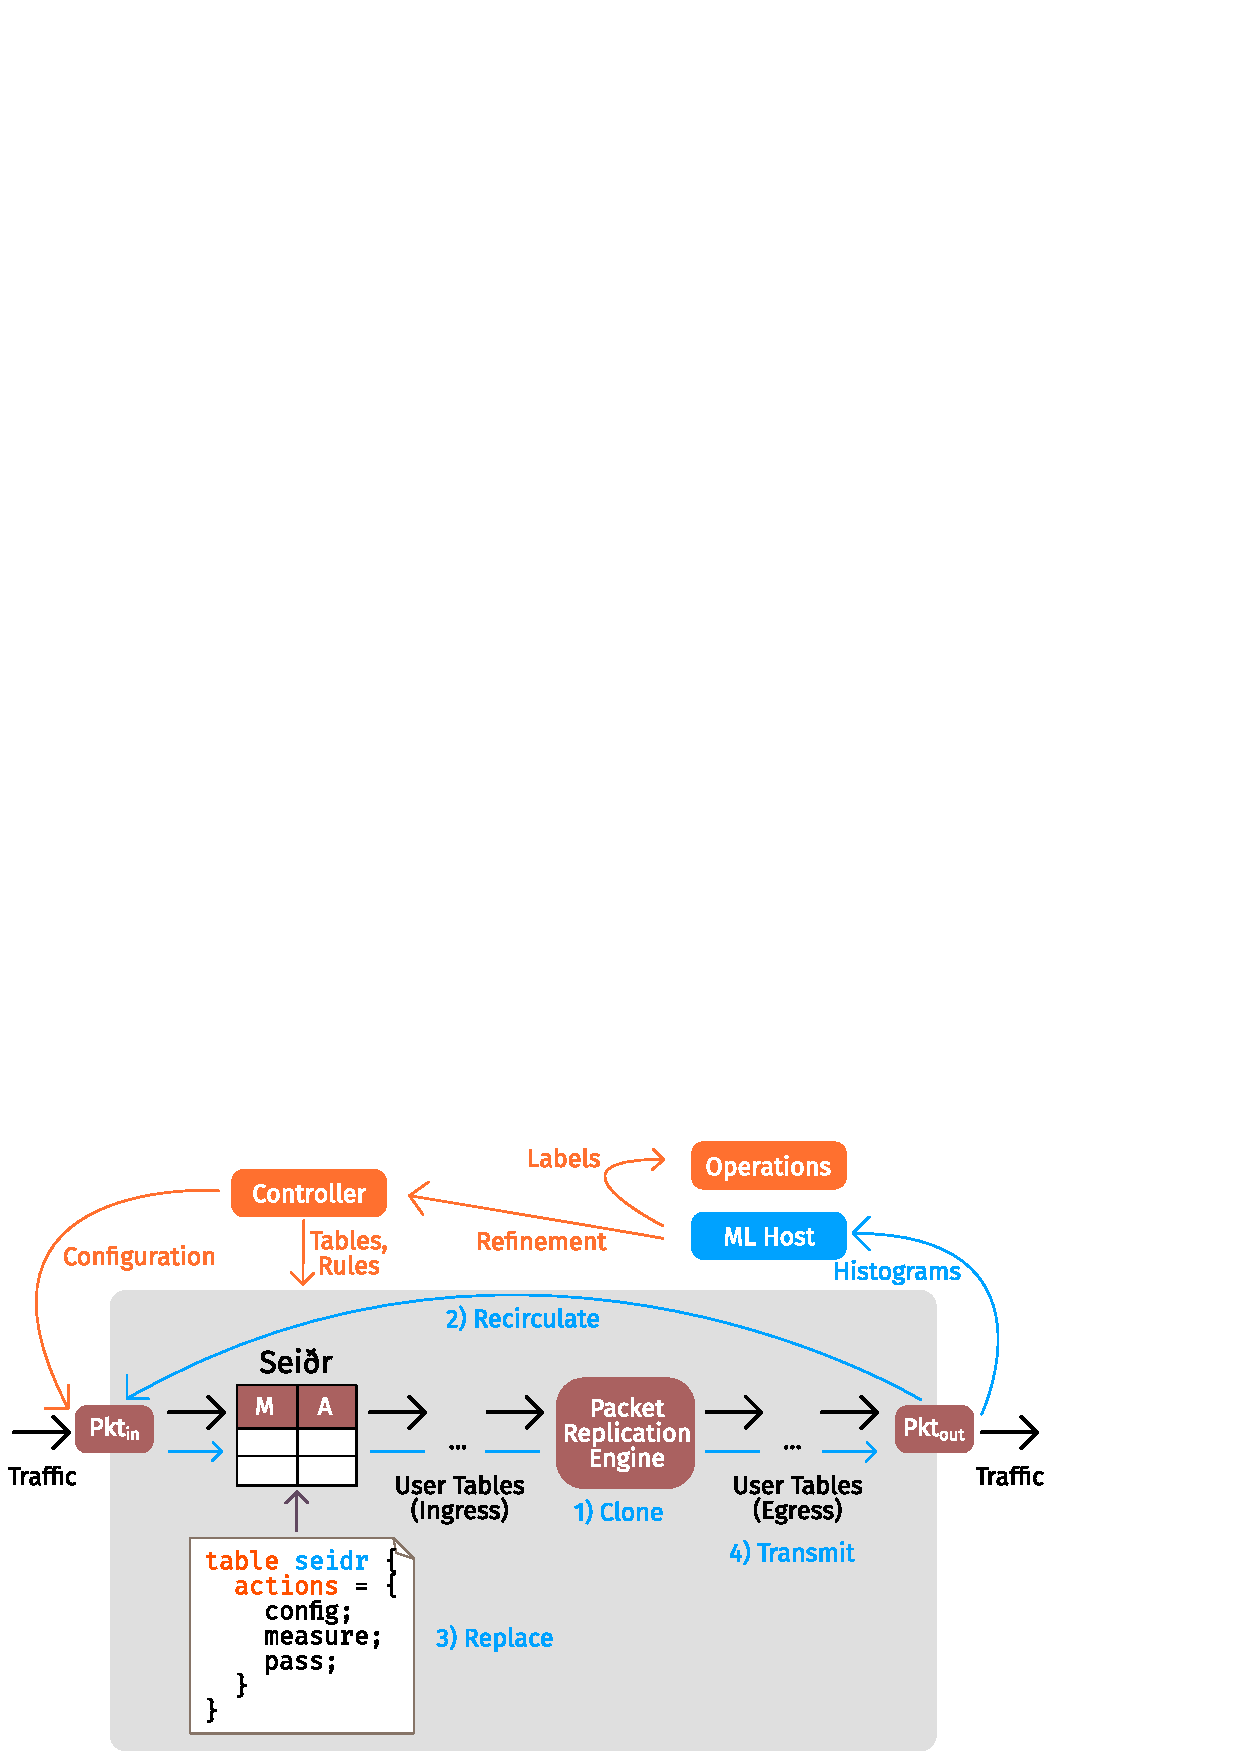
\includegraphics{diagrams/seidr/dp-arch-diagram.pdf}}
    \caption{\seidr{}'s integration with a PSA-compatible~\cite{p4-psa} dataplane.}
    \label{fig:arch}
\end{figure}

% Let's show them a histogram datastructure would look like purely with registers and how would a P4 action populate it - pseudocode or P4 snippet would be nice.

Although packet timing information is useful in understanding network and flow behaviour, without volume or packet rate reduction it is prohibitively expensive for hosts to handle each packet.
Histogramming acts as the \emph{aggregation step} which makes this class of analysis feasible in high-speed networks.
\Cref{fig:arch} demonstrates how \seidr{}, installed as an additional table in any P4 program, records and transmits inter-arrival time histograms.
The format for these histogram packets is outlined in \cref{fig:seidr-headers}; we choose to store individual buckets as \mintinline{rust}{u16}s, and the number of buckets in any histogram is fixed at compile time.
We set this to \num{100} buckets per histogram.
Packets traverse a table which requires \num{3} actions to be implemented:
\begin{enumerate}
    \item \mintinline{rust}{config} reads any matched packets as a \mintinline{rust}{seidr_cfg_t} of type \mintinline{rust}{SET_}\{ \mintinline{rust}{MIN}, \mintinline{rust}{MAX}, \mintinline{rust}{DST}, \mintinline{rust}{SRC}, \mintinline{rust}{LEN} \} by using the P4 parser.
    These update registers \numrange{1}{5} in \cref{tab:registers}, dropping any matched packets.
    
    \item \mintinline{rust}{measure} calculates the inter-arrival time, update per-flow histograms, and transmits finished histograms to the correct host. We describe its operation in \cref{alg:measure}.
    
    \item \mintinline{rust}{pass} ignores packets, and is the default action.
\end{enumerate}
Constructing \seidr{} in this manner allows the control plane to install rules to enable/disable runtime reconfiguration as needed, and to monitor as many or as few flows as desired (\ie, using wildcard rules, or exact matching).

The PSA does not have any mechanisms for generating new packets.
To circumvent this, any packet which would complete a histogram is tagged for cloning at the end of the ingress pipeline, and recirculation at egress (\cref{algline:recirc}).
This truncated copy returns to \seidr{}'s table, where we enable the relevant headers, change L2/3 fields, and write out the histogram contents (\crefrange{algline:rewrite-start}{algline:rewrite-end}).
The P4 deparser outputs the new protocol stack at egress, and transmits the histogram UDP packet into the network.
Event-driven architecture proposals~\cite{DBLP:conf/hotnets/IbanezABM19} may allow a more natural means of packet generation.

\begin{figure}
\centering
\begin{subfigure}{0.45\linewidth}
\centering
\adjustbox{max width = 0.6\linewidth}{
\begin{minipage}{\linewidth}
\begin{minted}[escapeinside=||]{rust}
|\textbf{\textcolor{Keyword}{header}}| seidr_cfg_t {
    bit<8> function;
    bit<144> payload;
}
\end{minted}
\end{minipage}
}
\end{subfigure}
\begin{subfigure}{0.45\linewidth}
\centering
\adjustbox{max width = 0.6\linewidth}{
\begin{minipage}{\linewidth}
\begin{minted}[escapeinside=||]{rust}
|\textbf{\textcolor{Keyword}{header}}| seidr_t {
    bit<128> src_ip;
    bit<128> dst_ip;
    bit<16> src_port;
    bit<16> dst_port;
    bit<16> eth_type;
    bit<BUCKETS * 16> histo;
}
\end{minted}
\end{minipage}
}
\end{subfigure}
\caption{P4 headers for \seidr{} configuration and histograms.}\label{fig:seidr-headers}
\end{figure}

\begin{algorithm}
% \vspace{-0.25cm}
% \DontPrintSemicolon
\KwData{5-tuple, P4 metadata, P4 headers, Registers}
h $\leftarrow$ hash(5-tuple)\;
index $\leftarrow$ BUCKETS * h\;
owner $\leftarrow$ HistoOwner[h]\;
\uIf{metadata.packet\_path = RECIRCULATE}{
    headers.tcp.valid $\leftarrow$ false\label{algline:rewrite-start}\;
    headers.udp.valid $\leftarrow$ true\;
    headers.seidr.valid $\leftarrow$ true\;
    copy 5-tuple into headers.seidr\;
    rewrite headers.ip, headers.udp using HistoSrc/Dest\;
    headers.seidr.histo $\leftarrow$ HistoData[index..]\;
    truncate payload\;
    zero out registers: BucketCount, HistoOwner[h], HistoData[index..]\;\label{algline:rewrite-end}
}
\ElseIf{owner = 0 \textbf{or} owner = 5-tuple}{\label{algline:owner-check}
    HistoOwner[h] $\leftarrow$ 5-tuple\;
    iat $\leftarrow$ LastTimestamp - metadata.mac\_ingress\_time\;
    \If{iat $\ge$ Min \textbf{and} iat $\le$ Max}{
        bucket $\leftarrow$ BUCKETS * (iat - Min) / (Max - Min)\;
        HistoData[index + bucket] $\leftarrow$ HistoData[index + bucket] + 1\;
        BucketCount[h] $\leftarrow$ BucketCount[h] + 1\;
        \If{BucketCount[h] = Len}{
            mark packet for cloning and recirculation\label{algline:recirc}\;
        }
    }
}

\caption{Histogram update and transmission.}\label{alg:measure}
\end{algorithm}

In the event of hash collision (\cref{algline:owner-check}), we ignore packets outside of the tracked flow to ensure that data is accurate.
As later processing and classification directly affect what decisions are made by operators or automatically taken by a policy (possibly leading to incorrect flow limits, QoS, \emph{etc.}), avoiding corruption/cross-contamination of operational data is paramount.
To gain collision resistance, Robin Hood hashing could be used up to a maximum distance in the table, treating a zeroed owner as empty and an illegal source IP as a tombstone value.

\begin{table}
    \centering
    \caption{Register map (Datatype, Amount) for an $h$-bit hash.}
    \resizebox{\linewidth}{!}{\begin{tabular}{@{}ccccccccc@{}}\toprule
        Min & Max & Length & HistoSrc & HistoDest & BucketCount & LastTimestamp & HistoOwner & HistoData \\ \midrule
        \mintinline{rust}{u16} & \mintinline{rust}{u16} & \mintinline{rust}{u16} & \mintinline{rust}{u16 + u128} & \mintinline{rust}{u16 + u128} & \mintinline{rust}{u16} & \mintinline{rust}{u64} & \mintinline{rust}{3 * u16 + 2 * u128} & \mintinline{rust}{BUCKETS * u16} \\
        1 & 1 & 1 & 1 & 1 & $2^h$ & $2^h$ & $2^h$ & $2^h$ \\ \bottomrule
    \end{tabular}}
    \label{tab:registers}
\end{table}

% Basic Logic:
% \begin{itemize}
%     \item table 1: three actions
%     \begin{itemize}
%         \item config: set R1 or R2 (controller installs rule matching a specific port/ip combo)
%         \item measure: take ingress timestamp from metadata, do stuff, write into lasttime, add to bucket and total if within bounds
%         \item pass (default)
%     \end{itemize}
%     \item then pass onto rest of tables
%     \item Why do it this way? can make it all or nothing through control plane.
%     \item How to write and send packet? Same trick as ESNET? (recirc w/ custom metadata to transform pkt)
% \end{itemize}

% ?? NOTE: See PSA \cite{p4-psa} for register format. Some papers, like Dapper, suggest that hash tables should be possible? That would work out very well in our benefit.

% ?? What is configurable? Min, max of the histogramming range

This design allows runtime configuration of all aspects save for the bucket count; at runtime, the only way to increase bucket resolution is to examine a smaller region of IATs.
While in theory this could be configured below a maximum compiled into the firmware, the difficulties introduced in classification/data processing make this infeasible.
Unless using stream-capable classifiers such as LSTMs~\cite{DBLP:journals/neco/HochreiterS97}, changing the input size requires retraining from scratch since new neuron weights must be added and structural properties of the input data change.
Increasing the bucket count requires new firmware installation, as many dataplane P4 implementations cannot allocate variable-length stores due to the lack of a dynamic allocator.

\begin{figure}[t]
    \centering
    \begin{subfigure}[t]{0.49\linewidth}
        \centering
        \resizebox{\linewidth}{!}{\includegraphics{plots/seidr/dt-cubic-1000-app.pdf}}
        \subcaption{TCP Cubic}
        \label{fig:cubic-hist-app}
    \end{subfigure}
    \begin{subfigure}[t]{0.49\linewidth}
        \centering
        \resizebox{\linewidth}{!}{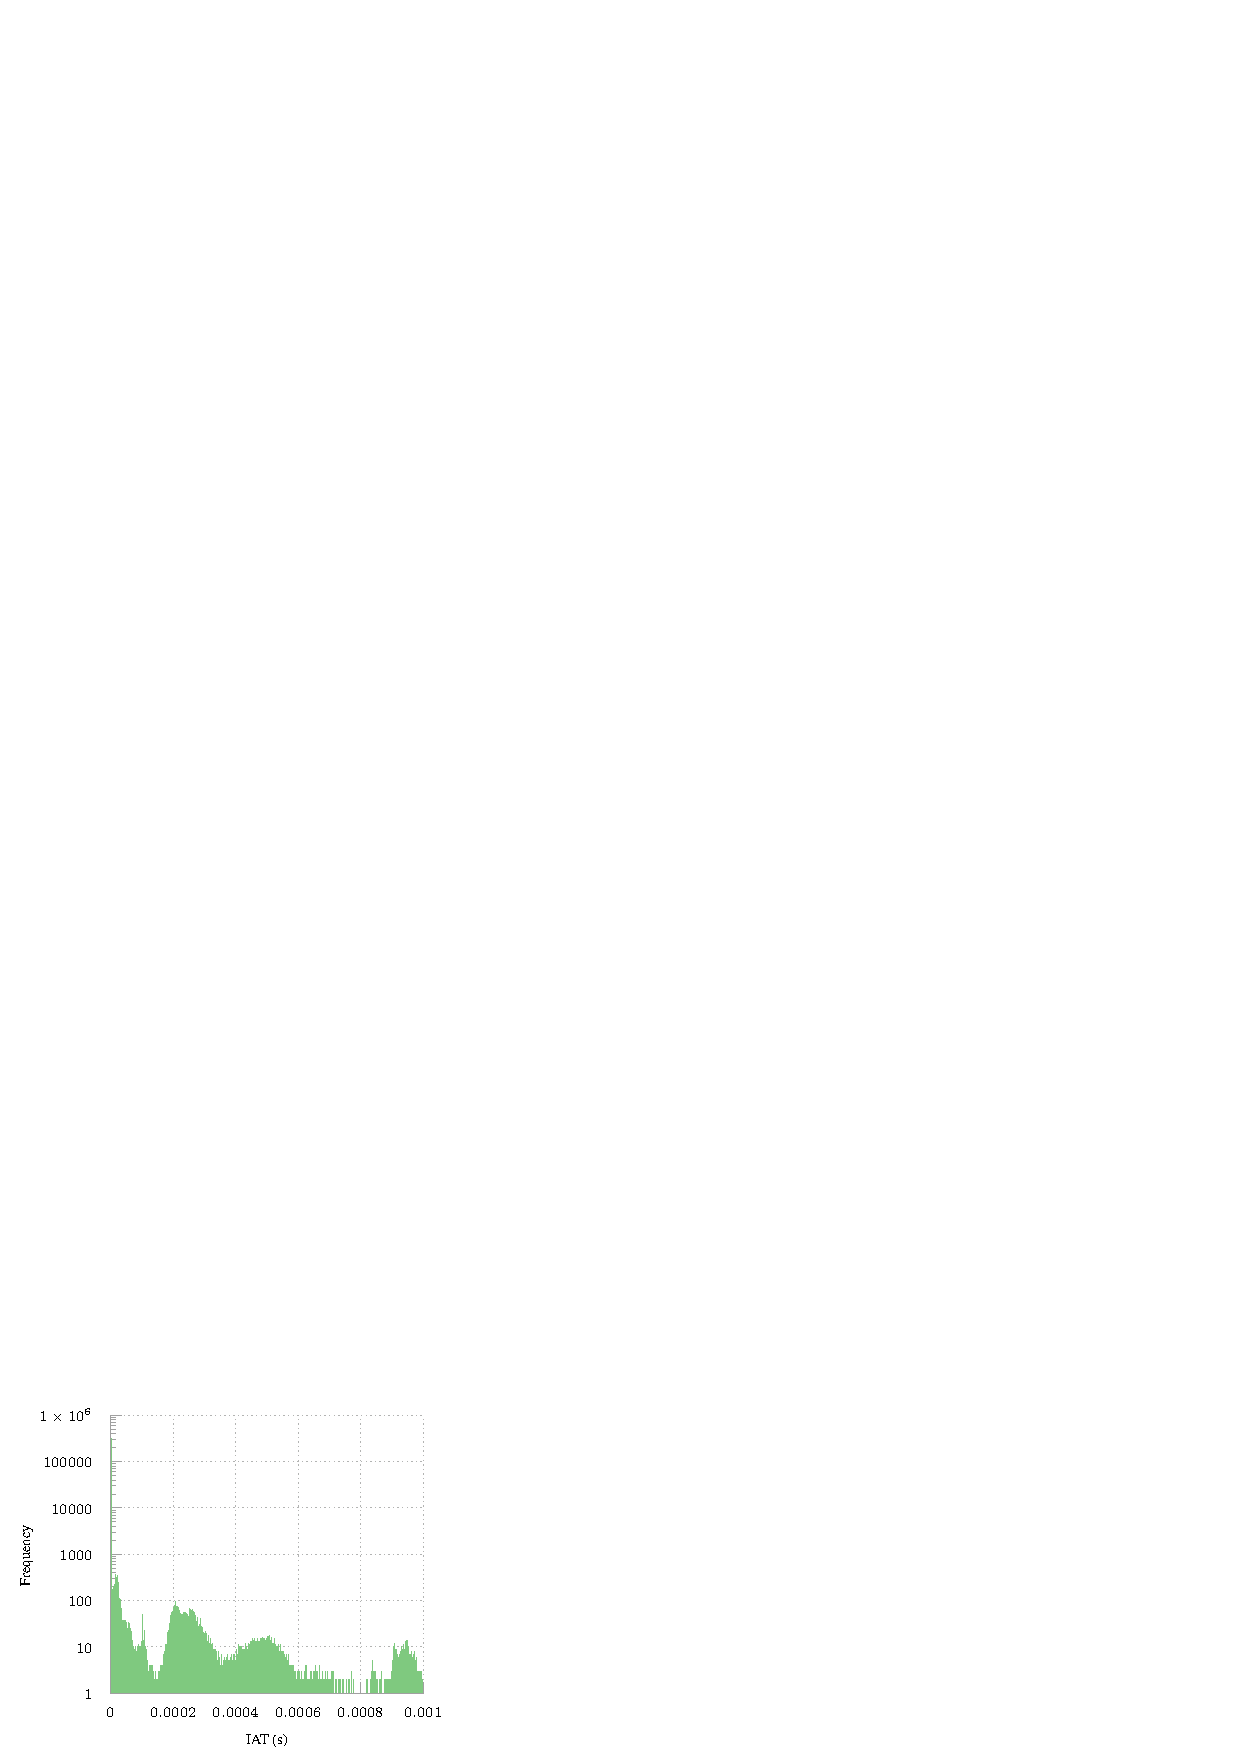
\includegraphics{plots/seidr/dt-bbr-1000-app.pdf}}
        \subcaption{TCP BBR}
        \label{fig:bbr-hist-app}
    \end{subfigure}
    \caption{Example dataplane histograms showing visible differences in inter-arrival times of selected TCP flavours. Our ML solutions are trained to programmatically identify such differences.}
    \label{fig:tcp-hist-app}
\end{figure}

As an example of dataplane-generated histograms, \cref{fig:tcp-hist-app} shows the distribution of inter-arrival times between two TCP congestion control algorithms. The visible differences are programmatically identified using our ML algorithms.

\subsection{Accurate, Precise and High-Resolution Timestamping}

Precise timestamps are critical when detecting temporal properties of flow behaviour, such as microbursts or inferring flow congestion control algorithms.
It is especially important in high speed (\SI{100}{\giga\bit\per\second}) networks, where there can be as little as \SI{6.7}{\nano\second} between packets that need to be analysed.
With a Linux-based software solution (\eg, reading packets from a link with \emph{tcpdump}), the Linux kernel can only provide microsecond-level accuracy with precision in the order of \SI{100}{\micro\second}~\cite{kundel2020p4sta}.
DPDK improves on this, increasing the accuracy to \SI{100}{\nano\second} in the best case~\cite{primorac2017measure}.
However, today's dataplane devices (\eg, Netronome SmartNICs, NetFPGA SUME) allow nanosecond-accurate timestamps to be retrieved from the \emph{Media Access Control} (MAC) modules with a precision of \SI{10}{\nano\second}~\cite{kundel2020p4sta}, a timestamp property \seidr{} relies upon.

% Some platforms provide picosecond-level precision and many solutions allow time synchronisation between multiple devices using the IEEE 1588-2002 (Precision Time Protocol) standard.



\section{TCP congestion control classification}\label{sec:seidr-tcpcc}


% We present an example of first-stage analysis performed for each flow and each packet---stateful TCP analysis.
% This includes numerous metrics which are considered standard when measured at connection endpoints, yet are difficult or invite numerous issues when performed in the network (of which we include a discussion on drawbacks and, curiously, benefits).
% The introduction of accurate timestamps allows us to explore rate-monitoring at a per-packet level, a new view of flow behaviour which may enable flow and hardware characterisation.

% \subsection{Per-Packet Rate Monitoring}

% \begin{figure*}
%     \centering
%     \begin{subfigure}[t]{0.49\linewidth}
%         \centering
%         \resizebox{0.5\linewidth}{!}{
% 	    \begin{tikzpicture}
%     		[packet/.style={draw, fill=uofgsunshine}]
% 		    \node[packet] (p1) {$p_1$: 1500B};
% 		    \node[packet, right= 1cm of p1] (p2) {$p_2$: 800B};
		
% 		    \node at ($(p1.south west) - (0,1)$) (t1) {$t_1$};
% 		    \node at ($(p2.south west) - (0,1)$) (t2) {$t_2$};
		
% 		    \draw[-, dotted] (t1.north)--(p1.south west);
% 		    \draw[-, dotted] (t2.north)--(p2.south west);
		
%     		\draw[<->] (t1.north) -- node[below]{$\mathit{dt}$} (t2.north);
% 	    	\draw[<->] ($(t1.north) + (0,0.2)$) -- node[above]{$s$} ($(t1.north) + (1.8,0.2)$);
% 		    \draw[<->] ($(t1.north) + (1.8,0.2)$) -- node[above]{$g$} ($(t2.north) + (0,0.2)$);
% 	    \end{tikzpicture} 
% 	}
%     \caption{\centering Per-packet rate, visualised. Note that $p_1$ and $p_2$ are not necessarily packets from the same flow.}
%     \label{fig:per-packet-rate}
%     \end{subfigure}
%     \begin{subfigure}[t]{0.49\linewidth}
%     \centering
%     \resizebox{0.9\linewidth}{!}{
% 		\begin{tikzpicture}
% 		[packet/.style={draw, fill=uofgsunshine}]
% 		\node[packet] (p1) {$p_1$: 1500B};
% 		\node[packet, right= 1cm of p1] (p2) {$p_2$: 800B};
% 		\node[right= 1cm of p2] (p3) {...};
% 		\node[packet, right= 1cm of p3] (p4) {$p_{n-1}$: 1500B};
% 		\node[packet, right= 1cm of p4] (p5) {$p_n$: 1500B};
		
% 		\node at ($(p1.south west) - (0,1)$) (t1) {$t_1$};
% 		\node at ($(p2.south west) - (0,1)$) (t2) {$t_2$};
% 		\node at ($(p4.south west) - (0,1)$) (t4) {$t_{n-1}$};
% 		\node at ($(p5.south west) - (0,1)$) (t5) {$t_{n}$};
		
% 		\draw[-, dotted] (t1.north)--(p1.south west);
% 		\draw[-, dotted] (t2.north)--(p2.south west);
% 		\draw[-, dotted] (t4.north)--(p4.south west);
% 		\draw[-, dotted] (t5.north)--(p5.south west);

%         \draw[<->] ($(t2.south) + (0,-0.25)$) -- node[above]{$s$} ($(t2.south) + (6.25,-0.25)$);
%         \draw[<->] ($(t2.south) + (6.25,-0.25)$) -- node[above]{$g$} ($(t5.south) + (0,-0.25)$);
% 		\draw[-, thick] ($(t2.south) - (0,0.5)$) -- node[below]{$W$} ($(t5.south) - (0,0.5)$);
% 		\end{tikzpicture} 
% 	}
%     \caption{\centering Sliding window rate, visualised. Rate estimates are computed using the sizes of the last $W$ packets seen in the current flow. Packets $p_2$ and $p_{n-1}$ belong to the same flow, but $p_n$ is not assumed to.}
%     \label{fig:sliding-window-rate}
%     \end{subfigure}
%     \caption{Comparison of per-packet and sliding window rates. The lengths of packets and inter-packet gaps are not to scale, and are purely demonstrative.}
%     \label{fig:pr-vs-slide}
% \end{figure*}

% Associating each packet with a high-resolution timestamp allows us to introduce the notion of a \emph{per-packet rate}.
% Assuming a packet with size $p$ arrives at time $t_1$ and is followed by another packet (potentially from another flow) which arrives at $t_2$, we measure $\mathit{dt}=t_2-t_1$ for this packet.
% Supposing this first packet spends time $s$ on the wire and assuming that the inter-packet gap $g$ is negligible compared to the length of a packet, then $\mathit{s} = \mathit{dt} - g \approx \mathit{dt}$.
% This packet then has a point rate, $r$:
% \begin{equation}
%     r = \frac{p}{s} \approx \frac{p}{\mathit{dt}}
% \end{equation}
% \Cref{fig:pr-vs-slide} demonstrates how this timing information arises, contrasted with sliding-window rate measurements taken over a longer time period.
% This assumes almost back-to-back traffic, which is realistic in our deployment environment, but to the best of our knowledge no programmable switches expose the timestamp at which the final bit of a packet has been ingested.
% Such a timestamp would allow exact measurement of $s$.

% % ?? we need to be clear about the unintuitive nature of these measurements, include a quick sketch proof which shows that the weighted average of a set of point rates is analytically identical to the sliding window rate/throughput taken over the same period of time.
% While this is an interesting measure to associate with each packet, considering how best to view such rates in aggregate can be counter-intuitive.
% Viewing these rates as time series data reveals interesting distributional characteristics which disagree starkly with our understanding of a flow's rate---for instance, clusters which suggest a different mean.
% Suppose we have a set of measurement indices $C$ with no gaps captured between $t$ and $t'$, partitioned into flows $C = F_1 \cup \dots \cup F_p$.
% To correctly combine a set of point measurements for a flow $F_i$ into an average rate $\overline{r}_{F_i}$, we compute:
% \begin{equation}
%     \overline{r}_{F_i} = \frac{\sum_{a \in F_i} \mathit{dt}_a r_a}{\sum_{c \in C} \mathit{dt}_c}.
% \end{equation}
% In the instance that only one flow is captured (\emph{i.e.}, $F_i = C$), this is a weighted average over point rates, using the $\mathit{dt}$ measured between each packet and the next packet in the same flow as its weight.
% Similarly, this is analytically equivalent to the sliding-window rate measured over the same set of packets:
% \begin{equation}
%     \frac{\sum_{a \in F_i} \mathit{dt}_a r_a}{\sum_{a \in F_i} \mathit{dt}_a} \simeq \frac{\sum_{a \in F_i} p_a}{t' - t}.
% \end{equation}
% % \begin{proof}
% % Given a set of contiguous measurements from the same flow $S \subseteq \mathbb{Z}$, admitting $p_s$, $r_s$, $\mathit{IAT}_s$ and $t_s$, the weighted average of point rates is then
% % $$
% % \overline{r}_S = \frac{\sum_{s \in S} \mathit{IAT}_s r_s}{\sum_{s \in S} \mathit{IAT}_s}
% % $$
% % The sliding-window average:
% % $$
% % \overline{r}_S = \frac{\sum_{s \in S} \mathit{IAT}_s r_s}{\sum_{s \in S} \mathit{IAT}_s}
% % $$
% % \end{proof}

% We assume that inter-packet gaps will be negligible (\emph{i.e.}, that the link is never in a state of very low utilisation), due to typically high utilisation on a WAN.
% % Similarly, we need to discuss the effects of selective monitoring or an abundance of UDP/ICMP traffic (which will distort $dt$s).
% However, this assumption can be distorted if selective TCP flow monitoring is used, or if UDP/ICMP traffic is overabundant; both these scenarios create larger gaps between TCP packets of interest, inflating $g$ to the point where it is comparable in size to $s$.
% This has an impact on our notion of per-packet rates, but not inter-arrival times or other such dependent metrics.
% The effect is small on sliding window rates, particularly at larger window sizes.
% ?? Justify. On paper, it looked like error term was O(1/n), O(g) for an n packet window.


% \section{Inter-Arrival Time}

% Having assigned each packet in a flow with a nanosecond-accurate timestamp ?? tbc

\Cref{fig:tcp-hist-app} suggests that a notable use-case for this type of measurement is \emph{congestion control algorithm} (CCA) detection.
In a TCP connection, each machine is free to choose the CCA it uses to send bytes, and thus how it responds to network congestion signals.
This choice is local, and so is invisible to the other machine (and the network).
In datacentre networks, operators choose these to ensure optimal behaviour.
In a transit network or large WAN however, these hosts (and thus the CCAs in use) are outside the control of network operators, which introduces difficulties when CCA interactions lead to \emph{unfairness}.
Consider the recent (and widespread) introduction of \emph{TCP BBR}~\parencite{DBLP:journals/queue/CardwellCGYJ16}.
\emph{BBR} is a delay/model-based CCA which converges on a fair share of bottleneck bandwidth by reducing its rate if the round-trip time increases, while periodically attempting to increase send rate to account for path/load changes.
However, \emph{BBR} traffic can consume \SI{40}{\percent} of link capacity when multiplexed with loss-based CCAs, regardless of the number of competing flows~\parencite{DBLP:conf/imc/WareMSS19}. 
When ensuring fair transit to all flows, this is hardly a desirable outcome; in fact, it's one which may frustrate clients or violate SLAs.

A curious property of \emph{BBR}'s algorithm which sets it apart from other variants is that packet transmission is \emph{timer-based}.
\texttt{send(packet)}, as defined in the canonical algorithm, asks that on transmission of a packet, the sender should wait for the estimated time that packet would take to reach the recipient.
For instance, at an estimated bottleneck bandwidth of \SI{8}{\mega\bit\per\second}, a \SI{1024}{\kilo\byte} packet would hold back the next packet in the flow until \SI{976.6}{\micro\second} had elapsed.
When packet sizes remain similar this causes strongly periodic behaviour, while mode switches in the \emph{BBR} algorithm cause these periodic bands to shift up or down accordingly.
This effect is stronger than in existing loss- and delay-based algorithms which remain intrinsically tied to the notion of a congestion window (where release of buffered packets follows the receipt of ACK messages).
As a result, timing behaviour of past CCAs may be influenced by (the lack of) packet pacing, periodic components might be made noisier by jitter along the return path, or the behaviour of the receiver might add further noise.

This high-level analysis of \emph{BBR} gives us a strong feature to use as the basis for classification: the \emph{inter-arrival times} (IATs) for each packet in a flow.
We have two options for processing this for classification: we may use a compressed, fixed-size representation such as histograms to capture the aggregate distribution, or we may attempt to capture structural behaviour by using a variable-length stream of IATs.
In many networks, the data and packet rate reduction offered by the former is required to make this possible.
Indeed, in-switch aggregation has seen great success in aiding ML for training~\parencite{DBLP:conf/isca/LiLYCSH19}, and direct execution~\parencite{DBLP:conf/hotnets/XiongZ19}.
We make use of the following standard classification algorithms on a fixed-size representation to attempt to single out the CCA in use:

\begin{itemize}
    \item \emph{$k$-Nearest Neighbours ($k$-NN)}. A simple and well-understood classifier which assigns labels based on the closest members of the training corpus (\ie, by the $L_2$ metric). Linear memory cost in amount of training data, and no training cost other than loading all data points, but capable of learning complex decision boundaries on fixed-length input.
    
    \item \emph{Convolutional Neural Networks (CNNs)}. A neural network approach which learns convolution kernels to classify fixed-length data, particularly when recognising spatial features. Memory cost is fixed for a given architecture irrespective of training data, with a high training cost.
\end{itemize}
% \fakepara{Long Short-Term Memory~\parencite{DBLP:journals/neco/HochreiterS97} units (LSTMs)} A class of recurrent neural network used for stream classification, forecasting, and prediction of variable-length data. Memory cost is fixed, with longer training times (and more data required) than similarly sized CNNs.
% Of these, we apply $k$-NN and CNNs to histograms of packet IATs, and LSTMS to raw IAT streams.

When examining $k$-NN classifiers, we measured accuracy across choices of $k \in \left[2, 8\right]$.
We found $k=2$ to be the most effective choice with our input data using the $L_2$ metric.
Our CNN architecture is described in \cref{tab:cnn-arch}, using ReLu activation and $1 \times 1$ stride in convolutional layers unless stated otherwise.
Training occurred over 5 epochs using the Adam optimiser with categorical cross-entropy as a loss metric, and a batch size of \num{64} histograms (\num{8} for full sequences due to the smaller data volume).
For \emph{BBR vs.\ Cubic}, the complete model consists of \num{104898} 32-bit floating-point parameters (\SI{409.76}{\kibi\byte}), while the full classification task adds a further \num{130} parameters (\SI{0.51}{\kibi\byte}).

\begin{table}
    \centering
    \caption{CNN architecture for \num{100}-entry histograms.}
    \resizebox{0.7\linewidth}{!}{\begin{tabular}{@{}cccc@{}}\toprule
        Layer & Nodes/Filters & Filter Size & Output Dimension \\ \midrule
        Conv2D & 32 & $(3 \times 1)$ & $(98 \times 1 \times 32)$ \\
        MaxPool & --- & $(2 \times 1)$ & $(49 \times 1 \times 32)$ \\
        Conv2D & 64 & $(3 \times 1)$ & $(47 \times 1 \times 64)$ \\
        MaxPool & --- & $(2 \times 1)$ & $(23 \times 1 \times 64)$ \\
        Conv2D & 64 & $(3 \times 1)$ & $(21 \times 1 \times 64)$ \\
        Flatten & --- & --- & \num{1344} \\
        Dense & 64 & --- & \num{64} \\
        Dense (Softmax) & $n_\mathit{classes}$ & --- & $n_\mathit{classes}$ \\
        \bottomrule
    \end{tabular}}
    \label{tab:cnn-arch}
\end{table}


\section{Evaluation}\label{sec:seidr-evaluation}
%Traffic is played back from hosts via Tcpreplay at a bandwidth assigned uniformly from a `good' or `bad' distribution, each using the same pcap file with source and destination IP addresses rewritten.

This work is most naturally compared against Marl, introduced by \textcite{DBLP:journals/eaai/MalialisK15}, the state-of-the-art in \gls{acr:rl}-based \gls{acr:ddos} prevention.
We are most interested in seeing how their approach contrasts with the new agent designs across different topologies and workloads.
Different network environments will also impose different levels of host density, where popular web servers may have orders of magnitude more clients than egress points from their network---I aim to show how these characteristics affect performance and learning rate.
Marl is known to outperform the AIMD~\parencite{DBLP:journals/ton/YauLLY05} strategy, yet the state of the art has long since moved on.
To paint a more current picture, I compare this work against an effective modern approach, \emph{SPIFFY}~\parencite{DBLP:conf/ndss/KangGS16}.
SPIFFY tests a proportion of flows by routing them through an alternate path with higher bandwidth, observing how their speed changes some time later.
This comparison lets us position our new agent designs against the state of the art, observing that SPIFFY has a similar mode of interaction to \gls{acr:rl}-based systems (taking action, observing an effect, and acting once again) and does not rely on protocol characteristics or signatures.
In reimplementing SPIFFY, I make the simplifying assumption that a suitable unused path exists (with identical bandwidth to the server's link).
\qty{10}{\percent} of active flows were tested at a time (according to the authors' observation that there is a factor of \qty{10}{\times} difference between the ideal and achieved bandwidth expansion), excluding flows below \qty{50}{\kilo\bit\per\second} and requiring a \qty{3}{\times} expansion from legitimate flows, making a judgement after \qty{5}{\second}.

To test this, I made use of both traffic models introduced in \cref{sec:a-new-normal} (Opus and \gls{acr:tcp}), both topologies discussed below (1-dest vs.\ Fat-Tree), and vary the amount of hosts typically communicating over each agent's ingress/egress node.
Additionally, these new models were evaluated in multi-agent mode (\emph{separate}, no model sharing), and in single-agent mode (\emph{single}, zero-cost perfect information sharing).
In each case, the algorithm's performance was averaged over \num{10} episodes of length \num{10000} timesteps (setting each agent's $\wvec{}=\mathbf{0}$ between episodes).
Host allocations at the beginning of each episode were generated pseudorandomly to ensure fairness between episodes---a host is malicious with probability $\operatorname{P}\left(\mathit{malicious}\right)$, and is benign otherwise.
Benign hosts generate traffic according to either \cref{sec:tcp-http-traffic-model,sec:udp-opus-traffic-model} depending on the experiment, while malicious hosts generate traffic as described in \cref{sec:attack-traffic-model} (both at experiment-dependent rates).

All experiments were executed on Ubuntu 18.04.2 LTS (GNU/Linux 4.4.3-040403-generic x86\_64), using an Intel Core i7-6700K (\qtyproduct[product-units=single]{4 x 4.2}{\giga\hertz}) which had \SI{32}{\gibi\byte} of \gls{acr:ram}.
%All code underpinning these findings is available on a public repository\footnote{\url{https://github.com/FelixMcFelix/rln-dc-ddos-paper}}.
%All code underpinning these findings is available on a public repository.\footnote{Private until publication.}

\subsection{Single destination}\label{sec:single-dest}
%?? Move description of tree topol to here.
The network is tree-structured, where one server $s$ connects through a dedicated switch to $k$ team leader switches, each connected to $\ell$ intermediate switches, which in turn each connect to $m$ egress switches.
We then have $N_{\mathit{hosts}} = k \ell m n$.
\Cref{fig:marl-topol} demonstrates this.
%Although \citeauthor{DBLP:journals/ccr/MahajanBFIPS02a}, the originators of this topology, make it clear that it exists as a fairly unrepresentative example \cite{DBLP:journals/ccr/MahajanBFIPS02a}, it remains the case that such a network topology allows for functional testing, and indeed is illustrative of one way in which attack traffic might aggregate in the network.
%It is hard, however, to argue its relevance to specific classes of victim or to reason about the interactions it might have with dependent applications.
%We aim to address this through \cref{sec:performance-in-an-emulated-environment}.
The network topology was configured using $k=2$ teams, $\ell=3$ intermediate nodes per team, $m=2$ agents per intermediate node, and $n \in \{2, 4, 8, 16\}$ hosts per learner.
This is a slight simplification of \Textcite{DBLP:journals/eaai/MalialisK15}'s \textquote{online} experiment, choosing fewer teams but remaining as a single server with a fan-out network.
%The algorithm parameters were set at $\gamma=0$ (leading to opportunistic behaviour), $\alpha=0.05$, having linearly annealed $\epsilon=0.2 \rightarrow 0$ by $t=3000$.
%Benign and malicious hosts uploaded between \SIrange{0}{1}{\mega\bit\per\second} and \SIrange{2.5}{6}{\mega\bit\per\second} respectively, and hosts were redrawn at each episode's start with $\operatorname{P}(\mathit{malicious})=0.4$.
%$U_s$  $k \ell mn+2$ \si{\mega\bit\per\second}.
%The performance of each choice of $n$ was averaged over \num{10} episodes of length \num{10000} timesteps (setting each agent's $\wvec{}=\bm{0}$ between episodes).
%Host allocations were generated pseudorandomly to ensure fairness between choices of $n$.
%These parameter choices match those of the original study to enable direct comparison, and are (to the best of our knowledge) arbitrary, but we justify our range of $n$ as capturing increasing scales of host activity.

\begin{figure}
	\centering
	\resizebox{0.9\linewidth}{!}{\begin{tikzpicture}[
	texts/.style = {text=black},
	labeltexts/.style = {text=uofgsandstone},
	treeline/.style = {draw=uofgburgundy},
	treenode/.style = {texts, circle, centered, fill=white, treeline},
	load/.style = {fill=uofgcobalt},
	loadhide/.style = {fill=uofgcobalt!40!white},
	external/.style = {fill=uofgrust},
	externalhide/.style = {fill=uofgrust!40!white},
	hideline/.style = {draw=uofgsandstone!40!white},
	hidenode/.style = {treenode, hideline},
	grow'=right
]
	\node[treenode, label={[texts]above:Server}] (root) {}
	child [treeline] { node [treenode, label={[texts]above:Core}] (sswitch) {}
		child [treeline] { node [treenode, label={[texts]above:Leader}] (teaml) {} 
			child [treeline] { node [treenode, label={[texts]above:Intermediate}] (inter) {}
				child [treeline] { node [treenode, load, label={[texts]above:Agent/Egress}] (agent) {}
					child [treeline] { node [treenode, external] (extern) {}
						child [treeline] { node [treenode, external, label={[texts]above:Host}] (host) {} }
						child [hideline] { node [hidenode, externalhide] (endhost) {} }
					}
				}
				child [hideline] { node [hidenode, loadhide] (endagent) {} }
			}
			child [hideline] { node [hidenode] (endinter) {} }
		}
		child [hideline] { node [hidenode] (endteaml) {} }
		edge from parent
		node[below, labeltexts] {$U_s$}
	};
	
	%\draw[-] (teaml) -- (endteaml);
	\node [labeltexts] (kdots) at ($(teaml)!0.5!(endteaml)$) {$\rvdots$};
	\node [labeltexts, right = -0.1cm of kdots] {$k$};
	\node [labeltexts] (ldots) at ($(inter)!0.5!(endinter)$) {$\rvdots$};
	\node [labeltexts, right = -0.1cm of ldots] {$\ell$};
	\node [labeltexts] (mdots) at ($(agent)!0.5!(endagent)$) {$\rvdots$};
	\node [labeltexts, right = -0.1cm of mdots] {$m$};
	\node [labeltexts] (ndots) at ($(host)!0.5!(endhost)$) {$\rvdots$};
	\node [labeltexts, right = -0.1cm of ndots] {$n$};
\end{tikzpicture}}
	\caption[Tree-structured network topology diagram for evaluating a single-destination network.]{
		Network topology diagram, showing how the server and its core switch's $k$ teams are structured, with $\ell$ intermediate routers per team, connected to $m$ agents which each moderate $n$ hosts beyond a single external switch.
		%	Empty nodes are considered to be internal.
		Red nodes are external, and each blue node hosts an agent.
		\label{fig:marl-topol}
	}
\end{figure}

\subsection{Multiple destinations}
The previous topology allows for direct comparison against the state-of-the-art, and indeed is illustrative of one way in which attack traffic might aggregate in the network.
It is hard, however, to argue its relevance to specific classes of victim or to reason about the interactions it might have with dependent applications.
In contrast, the fat-tree topology~\parencite{DBLP:conf/sigcomm/Al-FaresLV08} sees regular use in real-world data centres and scales well horizontally.
%?? Come up with description of fat-tree (multi-dest) topol.
%?? Why fat tree? regularly appears in modern datacentres.
%?? $k=4$ fat-tree , with one pod hosting two servers $s_0,s_1$.
We use a $k=4$ fat-tree, with one pod hosting two servers $s_0$ and $s_1$.
$n$ external hosts connect through each core switch (where agents are hosted), and communicate with $s_0, s_1$ uniformly randomly.
Both servers host identical services.
We set $n \in \{6, 12, 24, 48\}$ hosts per learner (keeping $N_{\mathit{hosts}}$ identical to each tier of the single-host topology), and restrict $U_{s_0} = U_{s_1} = U_s / 2$.

\subsection{Parameters}
The algorithm parameters were set at $\alpha=0.05$, linearly annealing $\epsilon=$ \num{0.2} $\rightarrow$ 0 by $t=$~\num{3000} in the case of Marl (\num{8000} actions per agent in the \emph{Instant/Guarded} models).

Benign hosts each occupied \qtyrange{0}{1}{\mega\bit\per\second}, and hosts were redrawn at each episode's start with $\operatorname{P}(\mathit{malicious})=$~\num{0.4}.
%The original introduction of this approach to direct-control reinforcement learning as introduced by \textcite{DBLP:journals/eaai/MalialisK15} fails to consider key cases: the absence of a suitable heuristic classifier $g(\cdot)$, disjoint ranges of traffic distribution (i.e., the presence of benign heavy-hitters), the accurate simulation of TCP-like behaviour (and its effects on collateral damage), and high densities of hosts at egress points.
%?? Why? ...
%Of these, the latter two are most deserving of a closer investigation, as they have stronger implications for wide-scale deployment.
%These are important issues, particularly when we consider real-world deployment.
%Heuristic estimates of traffic legitimacy come with computational cost and couple the reward function to the accuracy of the estimator, hosts often show diversity in their own traffic patterns (perhaps being multi-modal), and it is known that TCP is the most used transport protocol for Internet traffic \cite{DBLP:conf/saint/ZhangDJC09}.
%?? NEED TO VERIFY VOLUME OF CONGESTION-AWARE PROTOCOLS
Malicious hosts each sent \qtyrange{2.5}{6}{\mega\bit\per\second} when attacking \gls{acr:udp} traffic, though this was increased to \qtyrange{4}{7}{\mega\bit\per\second} when using \gls{acr:tcp}-like traffic (to meaningfully impact benign flows).
Given $n$ and $\operatorname{P}(\mathit{malicious})$, we see an expected malicious bandwidth \numrange{1.27}{1.87} and \qtyrange{2.03}{2.18}{\times} $U_s$ respectively.
%The expected fraction of $U_s$ consumed by each host is \SI{21.5}{\percent} for $n=2$, and \SI{2.84}{\percent} for $n=16$.
For these choices of $n$ in both topologies, we observe $N_{\mathit{hosts}} \in \left\{24, 48, 96, 192\right\}$, and an expected number of malicious hosts $\mathbb{E}\left[N_{\mathit{attackers}}\right] \in \left\{9.6, 19.2, 38.4, 76.8\right\}$.
For the largest choice of $n$, we see an expected total attack traffic $\mathbb{E}\left[V_{\mathit{attack}}\right] =$ \qtylist{334.05;422.4}{\mega\bit\per\second} for Opus and \gls{acr:http} traffic respectively.

$U_s$ was fixed at $N_{\mathit{hosts}}+2$ \unit{\mega\bit\per\second} (to account for burstiness), and each link had a delay of \qty{10}{\milli\second}.
All links had unbounded capacity, save for each server-switch.
These parameters match those of the original study to enable direct comparison, and many are (to the best of our knowledge) arbitrary, but I justify the range of $n$ as capturing increasing scales of host activity.

% \section{Related Work}\label{sec:related}
% %?? Try and compare my work here when possible?

\fakepara{DDoS Prevention}
\Textcite{DBLP:conf/lcn/BragaMP10} examine the detection of flooding DDoS attacks through \emph{self-organising maps}, using SDN to gather statistics effectively.
Many of their features aren't overly relevant, as their focus is not active defence or discovering \emph{which} hosts contribute to an attack.
%?? Actually talk about Marl (???) to appease reviewer \#1.
The closest available approach within this field is that of \textcite{DBLP:journals/eaai/MalialisK15} (whom we have positioned our work against), and their contribution in applying RL to the task of intrusion prevention is significant: their work helps to show the viability of live, adaptive, feedback-loop-like control of the network to detect and prevent DDoS attacks.
They create a tree overlay topology (subdivided into teams), where each agent applies packet drop to \emph{all} flows inbound to a protected server.
%?? Recap their flaws, since they've been cut form every other aspect.
Our results show that their technique underperforms at high host density and when congestion-aware traffic dominates---that their results do not demonstrate this suggests an evaluation driven purely by traces (rather than live application dynamics).

\emph{SPIFFY} \cite{DBLP:conf/ndss/KangGS16} aims to remedy transit-link attacks by observing how flows from each source respond to a sudden increase in available bandwidth.
\Citeauthor{DBLP:conf/ndss/KangGS16} realise that bots participating in an attack are often unable to match this bandwidth expansion (having already saturated the capacity of their outbound links), while legitimate flows typically speed up to match the new fair-share rate.
%Attackers must either be detected or reduce the throughput of each bot, increasing the cost of launching an attack.
%Unlike our approach (and due to the class of attacks it is designed to defend against), SPIFFY is intended to be deployed within ASes, although .
A weakness of their approach is that computing a route to measure bandwidth expansion on real networks can be costly (up to \SI{14}{\second} for the Cogent topology), and that the low expansion factors in real network can require more ``rounds'' of filtering.
By contrast, our approach takes a constant time to compute an action for a flow regardless of topology size.
Their assumptions about traffic response to such bandwidth expansion do not hold for constant bitrate flows (e.g., VoIP) and may not extend to HTTP DASH flows, both of which make up a sizeable proportion of network traffic.

\emph{Athena} \cite{DBLP:conf/dsn/LeeKSPY17} is a generalised SDN framework for intrusion detection, but has shown the use of a \emph{k-nearest neighbours} classifier to detect individual attack flows.
Although heavyweight (and proven to be effective compared with \textcite{DBLP:conf/lcn/BragaMP10}), their comparison against SPIFFY lacks the quantitative evidence required to understand how the system compares.
\Textcite{DBLP:conf/sp/SmithS18} use AS-level routing to tackle both transit-link and flooding-based attacks.
This view is taken due to the perceived cost of per-stream classification and inherent sensitivity to adversarial examples.
The approach is creative, relying upon BGP \emph{fraudulent route reverse poisoning} to preserve traffic to a target AS, but unlike SPIFFY the approach doesn't actually \emph{remove} the congestion.
Because of this, flooding-based attacks aren't fully alleviated.

%?? Abuses of RL 
\fakepara{RL in Networks}
Earnest, well-considered application of RL towards the challenge of intrusion prevention has seen comparatively little examination.
Past work treats the paradigm as a traditional classifier for anomaly detection \cite{shamshirband2014anomaly} and DDoS prevention \cite{DBLP:conf/mates/ServinK08}.
Given that the main strengths of RL techniques are the ability to control ongoing interaction and adapt by observing the concrete effects of actions, such works don't apply the rich literature on the subject to its fullest potential.

For categorising how RL fits into solving problems, we label works as direct- or indirect-control RL.
A \emph{direct-control} RL problem is one where the RL agent(s) learn optimal control over a set of actions as the \emph{primary} defence or decision-maker---requiring measurements, reward functions and action sets tailored for this purpose.
%We feel there is a shortage of work in this category at present, at least in the field of networks.
To date, the best-fitting example we have encountered is that of \textcite{DBLP:journals/eaai/MalialisK15}.
An \emph{indirect-control} RL problem is one where agents act in service to \emph{another technique} responsible for decision-making, optimising or generalising aspects of its operation beyond that of hand-coded heuristics.
A past example includes learning when best to share knowledge between \emph{hidden Markov model} anomaly detectors \cite{DBLP:conf/paisi/XuSH07}.
%The position of this work is weakened by its reliance on the problematic `DARPA99' dataset \cite{DARPA-IDD, DBLP:conf/cisda/TavallaeeBLG09, DBLP:conf/sp/SommerP10}, but the idea itself is well-treated and this acts as a driver for improvements in this direction.
This work is weakened by its reliance on the problematic `DARPA99' dataset \cite{DBLP:conf/sp/SommerP10}, but the idea itself is well-treated.
Outside of intrusion detection, there has been growing interest in the use of RL in data-driven networking, such as for intra-AS route optimisation \cite{DBLP:conf/hotnets/ValadarskySST17} and resource-constrained process allocation \cite{DBLP:conf/hotnets/MaoAMK16}.
\textcite{DBLP:conf/sigcomm/MaoNA17} employ client-side observations of network state and video performance with RL to optimise bitrate selection for multimedia streaming.
\emph{AuTO} \cite{DBLP:conf/sigcomm/ChenL0L18} employs deep RL to perform traffic optimisation.
Crucially, they find that the vast majority of flows are short-lived, requiring effective decisions in less than a millisecond.
To overcome the high latency of action computation via a neural network, two agents are trained, handling aspects of short and long flows respectively.
The first learns to optimise the flow size thresholds to demarcate long and short flows; these short flows are routed by ECMP.
The second agent makes bespoke decisions about routing, prioritisation etc.\ for each of the remaining long flows.


\section{Summary}\label{sec:seidr-conclustion}
We have presented \seidr{}, a dataplane assisted flow classification solution that can be used to detect fine-grained temporal flow behaviour. We have shown a PSA-compliant way to implement in-network data aggregation in the form of histograms, while using nanosecond-precision timestamping. Our in-network generated histogram datastructure (\eg, on per-flow packet inter-arrival times) has been presented as the input for various ML algorithms, including CNN and $k$-NN. We have shown with our extensive evaluation that \seidr{} can successfully tell apart TCP CCAs, in particular, it identifies BBR from its predecessors with over \SIrange{88}{96}{\percent} accuracy, while only consuming a maximum \SI{15.5}{\mebi\byte} of dataplane memory. We presented the trade-offs between training and inference times, memory requirements, and accuracy in the context of CNN and $k$-NN classifiers and shown that \seidr{} outperforms prior work by increasing classification accuracy on novel TCP CCAs, providing the ability to classify at very high traffic rates (in the order of \SI{10}{\tera\bit\per\second}).
Furthermore, we have identified a key temporal property of \emph{BBR} which allows its easy detection among other flows.
In the future, we aim to examine the use of \seidr{} towards microburst detection and diagnosis~\cite{DBLP:conf/sigcomm/ChenFKRR18} and for the identification of \emph{BBR}-like temporal properties of emerging UDP-based congestion-aware protocols, such as \emph{QUIC}.%~\cite{DBLP:conf/sigcomm/LangleyRWVKZYKS17}.

?? Through this chapter, we have discussed ..., lending credence to one of the claims in my thesis statement: \superrecallthesis{3}

\chapter{Scalable Flow Classification}\label{chap:seidr}

% \section{Motivation}
% \section{Sei\dh{}r Histograms}
% \subsection{Algorithm}
% \subsection{Packet Generation on PSA}
% \section{Use case: TCP CCA Detection}
% \subsection{Observable Differences}
% \subsection{Investigating the BBR Algorithm}
% \section{Methodology}
% \subsection{Testing Environments}
% \subsection{Data Collection/Generation}
% \subsection{ML Model Architecture}
% \section{Evaluation}
% \subsection{Device Memory Costs}
% \subsection{Bandwidth Costs}
% \subsection{CCA Detection Accuracy and Costs}

?? Problem statement: damn, all this ML is cool
?? We can do cool real-time analysis of operational Internet traffic
?? What do we do if we need more complex ML models: i.e., need to use LSTMs, or complex CNNs because we need to make use of complex temporal or structural features of data? We still need to get it to host machonies.
?? Okay... but in that case, how can we reduce data so that PPS and Gbps of data don't overwhelm the host, or that we lose lots of asid data and make poor decisions when we have many (or very fast) flows?

?? Relate some of this \emph{specifically} back to discussion of flow measurement in the dataplane in the INC use-cases? (i.e., considering all th below IPfix, sFLow, etc. etc.)
?? Try to relate some of the same problems.

There has been significant research and development on real-time analysis of operational Internet traffic.
Accurate flow characterisation (or \emph{classification}) can drive intrusion detection, detecting unusual or illegal patterns of network traffic, or to prioritize traffic for certain customers, to provide path-diversity as well as to mark Quality of Service (QoS) of various users and protocols~\parencite{DBLP:journals/ccr/BernailleTASS06,DBLP:conf/lisa/Roesch99}.
However, flow classification solutions today can usually only rely on sampled data provided by routers, such as sFlow, Netflow, or IPFIX, along with imprecise timing (\si{\micro\second} and \si{\milli\second}-level)~\parencite{rfc7011,rfc3954}.
While sampled, low-precision telemetry can be used to classify network traffic based on some flow properties (such as port and protocol numbers)~\parencite{DBLP:conf/iwcmc/RossiV10}, it cannot be used to classify based on fine temporal properties (\eg, identifying bursty flows and senders that can cause microbursts and buffer overflow on the network).

On the other hand, full-software solutions for traffic classification have been proposed by commercial vendors (\eg, Barracuda DPI\footnote{https://www.barracuda.com/glossary/deep-packet-inspection}), the open-source community (\eg, Snort~\parencite{DBLP:conf/lisa/Roesch99}, Zeek (formerly Bro)~\parencite{DBLP:conf/uss/Paxson98,zeek}), and the research community, with extensible feature sets and algorithms for classification~\parencite{DBLP:conf/icccn/HagosEYK18}.
Unfortunately, these software solutions designed for commodity hardware do not provide accurate timing of packets, and therefore make certain time-critical events hard or impossible to detect (\eg, microbursts~\parencite{DBLP:conf/sigcomm/ChenFKRR18} or congestion control properties~\parencite{DBLP:conf/icccn/HagosEYK18}).
Moreover, even the most sophisticated software solutions process packets orders of magnitude slower than current backbone traffic of large operators, making them unusable for large-scale operational analysis~\parencite{DBLP:journals/wpc/ParkA17}.

At the same time, programming and fast reconfiguration of network devices is being explored in all types of networks: datacenter and cloud networks, CDNs and WANs.
Specifically, with the recent developments of generalized dataplanes (\eg, the \emph{Portable Switch Architecture}~\parencite{p4-psa}), target devices (\eg, Barefoot Tofino and Netronome SmartNICs) along with the high-level programming languages presented for them (\eg, P4~\parencite{DBLP:journals/ccr/BosshartDGIMRSTVVW14}), operators can now express in-network functionality running on their devices, including accurate nanosecond-precision packet timing.
However, programming in-network services has its own challenges (\eg, restricted instruction sets, data types and memory), prohibiting the implementation of a fully in-network classification solution.

% To solve the aforementioned challenges, this paper presents an architecture that marries the precision timing and fast data aggregation capabilities of the dataplane with software classifiers that can run complex classification models due on a the reduced data rate.

To solve the aforementioned challenges, we present \seidr{}\sidenote{Pronounced ``SAY-ther''. ?? Explain naming?}, a dataplane assisted flow classification solution.
Our design philosophy of \seidr{} keeps functionality where it belongs: dataplane devices create accurately timestamped, aggregated data structures for our analysis, and we let a scalable software stack perform ML-based classification on commodity machines.\sidenote{?? Yeah this directly contradicts the main theme and line of reasoning of my thesis LMAO}
As in-network aggregation reduces the data rate by a factor of $\sim$\num{740}, our solution can analyse aggregated data from a total rate of \SI{10}{\tera\bit\per\second} original traffic using a single commodity processing machine.

As a concrete use-case, we look at fine dynamics of TCP congestion control algorithms.
Understanding and classifying them is important for network providers as inadequate choices have severe effects on transfer rates, especially in networks with high bandwidth-delay product~\parencite{DBLP:journals/queue/CardwellCGYJ16} and in networks where multiple congestion control algorithms are used~\parencite{DBLP:conf/imc/WareMSS19}. 
By using accurate congestion control diagnostics, operators will be able to infer sender problems (\eg, backlogged or application-limited senders), network inefficiencies (\eg, increased path latency and congestion), as well as receiver issues (\eg, delayed acknowledgements, small receiver windows) and fairness issues between delay-based and loss-based algorithms~\parencite{DBLP:conf/imc/WareMSS19}.

The contributions of this paper are summarized below:
\begin{itemize}
	\item A flexible dataplane-assisted architecture compatible with the \emph{Portable Switch Architecture} (PSA)~\parencite{p4-psa} that allows data aggregation in the form of histograms with nanosecond-accurate timing (\Cref{sec:architecture}),
	\item A high-accuracy method for telling apart timer-based (\eg, BBR) and cwnd-based TCP flavours using our system with machine learning algorithms (\Cref{sec:tcpcc}),
	\item An extensive evaluation of TCP congestion control classification using our solution (\Cref{sec:evaluation}).
\end{itemize}

The work presented in this chapter considers how \gls{acr:pdp} hardware can reduce input, though fine-grained, measurements into digests suitable for \gls{acr:ml} models running on host machines, and is based upon \citetitle{DBLP:conf/globecom/SimpsonCP20}~\parencite{DBLP:conf/globecom/SimpsonCP20}.
?? Then summarise contents from here...

?? Big open qs:
?? relevance of PSA digests? These can emit packets, no? These can emit an arbitrary struct to the ctl plane over P4Runtime API. Might be good if no digest support, . Digests have a few extra benefits: In some dataplanes can be emitted in egress. Is message fusion a possible downside? (unpredictable)
?? Maybe 2 options? Can be in-band or out-of-band. Digests are the out-of-band option, meanwhile in-band allows you to use dataplane to forward to accelerators like BrainWave (don't add extra load to ctl plane in this way?)

?? Header size limits are the other main constraint.
?? THis is probably not a problem with digests.
?? WHen emitting to dataplane, however? Will have plat-dependent limits on output. Header size limits, PHV limits, register access reqs that could prevent digest access? Need to mark in-progress histo emissions, progress for each, and emit bitslices spread over multiple egress pkts. Logic: CLONE LOOP WHile still pkts to write, block updates to histo if progress (1 bit?). Limitation: Histo emission freq must be reduced to prevent massive traffic amp. slicing logic could be extended to include the digest case? Are there PHV limits in the digest case that make this really suck?

%\section{Introduction}\label{sec:seidr-introduction}
%Network anomaly detection and intrusion detection/prevention are continually evolving problems, compounded by the partial, non-\emph{independent and identically distributed} (IID) view of data at each point in the network.
Attacks and anomalous behaviours evolve, becoming more sophisticated or employing new vectors to harm a network or system's confidentiality, integrity, and availability without being detected \cite{DBLP:journals/comsur/BhuyanBK14}.
These attacks and anomalies have measurable consequences and symptoms which allow a skilled analyst to infer new signatures for detection by misuse-based classifiers, but unseen attacks may only be defended against after-the-fact.
This issue is inherent to \emph{misuse-} or \emph{signature-based} intrusion detectors, and it has been long-hoped that \emph{anomaly-based} detectors would surpass this by making effective use of statistical measures \cite{DBLP:journals/comsur/BhuyanBK14}.

While \emph{machine learning} (ML) approaches seem like a sensible fit for this problem, in \citeyear{DBLP:conf/sp/SommerP10} \citeauthor{DBLP:conf/sp/SommerP10} identified the `failure to launch' of ML-based anomaly detection systems---a distinct lack of real-world system deployments \cite{DBLP:conf/sp/SommerP10}.
To quite a large extent, this remains the case today.
They posit that their use is made difficult due to significant operational differences from standard ML tasks, including: the high cost of errors and extraordinarily low tolerance for false positives inherent to network intrusion detection \cite{DBLP:conf/ccs/Axelsson99}; a general lack of recent, openly available (and high-quality) training data; and diversity of network traffic across varying timescales combined with significant burstiness \cite{DBLP:journals/ccr/LelandWTW95}.
Above the aggregate level, the constant deployment of new services and protocols means that traffic is \emph{non-stationary} and displays an evolving notion of normality.
Learning is made harder still by the challenges encountered with unlabelled (often partial) data.
All of these factors greatly inflate the difficulty of the detection problem.

%?? Make it clearer here what problem I specifically want to solve: principally a particular class of DDoS attacks; volume-based DDoS attacks. Amplification attacks are just a specialisation, this can be made more obvious. I think I need to be clearer about the \emph{intended deployment environment} of service hosts (i.e., not ISPs).

For certain classes of problem e.g., volumetric \emph{distributed denial of service} (DDoS) attacks, \emph{reinforcement learning} (RL) offers another perspective.
%?? Unclear explanation of RL here?
RL agents operate by following a \emph{policy} to interact with or control a system, while at the same time using observed performance metrics and deliberate exploration to dynamically improve this policy.
In this way the role of a RL agent differs from that of a standard classifier, adaptively reacting to threats by assuming the role of a feedback loop for network optimisation, typically to safeguard service guarantees.
In a sense, this allows us to ``overcome'' some of the difficulties of the detection problem by monitoring \emph{performance characteristics and consequences} in real-time; by looking for (and controlling) the effect rather than the cause.
Long-term, we expect that the value of RL-based defence systems will be to augment what existing misuse-based solutions can provide, by automatically alerting, recording and controlling what are believed to be illegal system states.
The goal of this work is much less general; we aim to prevent volume-based DDoS attacks with the aid of RL-based techniques (an important goal in its own right), while bringing to light the flexibility and applicability of these techniques in the security domain.
%Whether it takes direct control of the network, or is used indirectly to optimise a key part of another system, more powerful `deep' RL techniques (and well-founded action spaces) aren't yet well explored for network IDS/IPS.
%These range from more modern training algorithms \cite{DBLP:journals/corr/SchulmanWDRK17, DBLP:conf/icml/SchulmanLAJM15}, to evolutionary strategies \cite{DBLP:journals/corr/SalimansHCS17, DBLP:journals/corr/abs-1802-08842}, hierarchical action composition \cite{DBLP:journals/corr/abs-1710-09767}, and competitive multi-agent learning \cite{DBLP:journals/corr/abs-1710-03748}.

To date, there have been few applications of this class of algorithms towards intrusion detection and prevention which make use of their full potential for online control, rather than using them as the basis for a classifier.
We aim to take steps to redress this and establish their proper capabilities, beyond simple ``blind application''.
%?? Expand as required
What approaches do exist are aimed towards the task of adaptive online DDoS mitigation, and rely upon learning to control probabilistic packet drop.
%?? THAT IS A MAJOR CONTRIB, MENTION IT EVERYWHERE YOU CAN

%?? Discuss the most important conclusions before the outline.
We find that the existing work for this task \cite{DBLP:journals/eaai/MalialisK15} fails to account for congestion-aware traffic (i.e., TCP) and environments with high host density per egress point, achieving poor results due to an overly coarse view of the network.
To remedy this, we make throttling decisions on a per-source basis and present the engineering decisions this mandates: updating RL agents from multiple traces per timestep, timed random sequential action computation and a supporting \emph{software-defined network} (SDN) architecture.
In tandem with the development and evaluation of an effective state space and model, we provide the design of a second model inspired by past work on algorithmic DDoS prevention, as an example of the integration of domain-specific knowledge.
Our introduction of per-source decisions improves substantially upon the state-of-the-art when acting upon most internet traffic (i.e., congestion-aware protocols), and we show that our second model achieves excellent performance for high host density in this case.
Crucially, both models remain protocol- and content-agnostic to offer future-proofing against the rollout of future protocols like QUIC \cite{DBLP:conf/sigcomm/LangleyRWVKZYKS17}.
%?? Also algorithmic enhancements such as multiple actions per timestep, 
%?? PROTOCOL-AGNOSTIC -- HOW WILL THESE THINGS COPE WITH QUIC ET AL.?!?!

\subsection{Contributions}
This paper contributes two source-level granularity approaches to RL-driven DDoS prevention (\emph{Instant} and \emph{Guarded} action models), improving upon past aggregate-based models (\cref{sec:ddos-mitigation-with-per-flow-reinforcement-learning}).
These are designed to make effective decisions irrespective of protocol, and act on individual flows at the edge of any network topology.
We offer an in-depth investigation into suitable features for automatic DDoS mitigation, with qualitative and quantitative justification (\cref{sec:rethinking-the-state-space}).
These features have been suggested by past studies, and independently tested in their own contexts.
Our study is the first attempt to quantify the individual efficacy of each in an RL setting.

We implement reactive simulations of HTTP and VoIP web-server traffic, designed to test system characteristics that packet trace playback fails to capture (\cref{sec:a-new-normal}).
To our knowledge, this is the first attempt to study or replicate Opus-based VoIP traffic, which has become commonplace since the codec's release in 2012.
These new traffic models inform an empirical evaluation of our new models against the state-of-the-art in RL-based DDoS mitigation using (\cref{sec:the-results-of-doing-so}), alongside a discussion of security concerns and real-world deployment (\cref{sec:discussion}).
We additionally compare our work against SPIFFY \cite{DBLP:conf/ndss/KangGS16}, reuniting two divergent strands of research and grounding the study of RL-based DDoS defences.

\section{Telemetry creation in the dataplane}\label{sec:seidr-architecture}


%  No need for this... space issues
% \begin{figure}
%     \centering
%     \resizebox{0.7\linewidth}{!}{\includegraphics{plots/Hyllus-architecture.pdf}}
%     \caption{Architecture (placeholder).}
%     \label{fig:arch}
% \end{figure}

% As shown on Figure~\ref{fig:arch},



\subsection{Limitations of Programmable Dataplanes}
While dataplane programming promises easy reconfiguration of network devices, it poses some challenges.
First, network devices support only a limited set of operations and control flows (no loops) without use of platform-specific \mintinline{rust}{extern}s, and restrict the user to specific primitive data types, \ie, no floating-point units due to tight hardware constraints.
Second, these devices have limited low-latency memory (on the order of a few tens of \si{\mega\byte}s~\cite{jin2017netcache}) and do not provide dynamic memory management.
These limitations prohibit complex algorithms from being implemented, but allow certain restricted solutions, such as what is presented in DAPPER~\cite{DBLP:conf/sosr/GhasemiBR17}, where the authors implement a TCP state machine purely in the dataplane.

\subsection{Histogram Generation}

\begin{figure}
    \centering
    \resizebox{0.8\linewidth}{!}{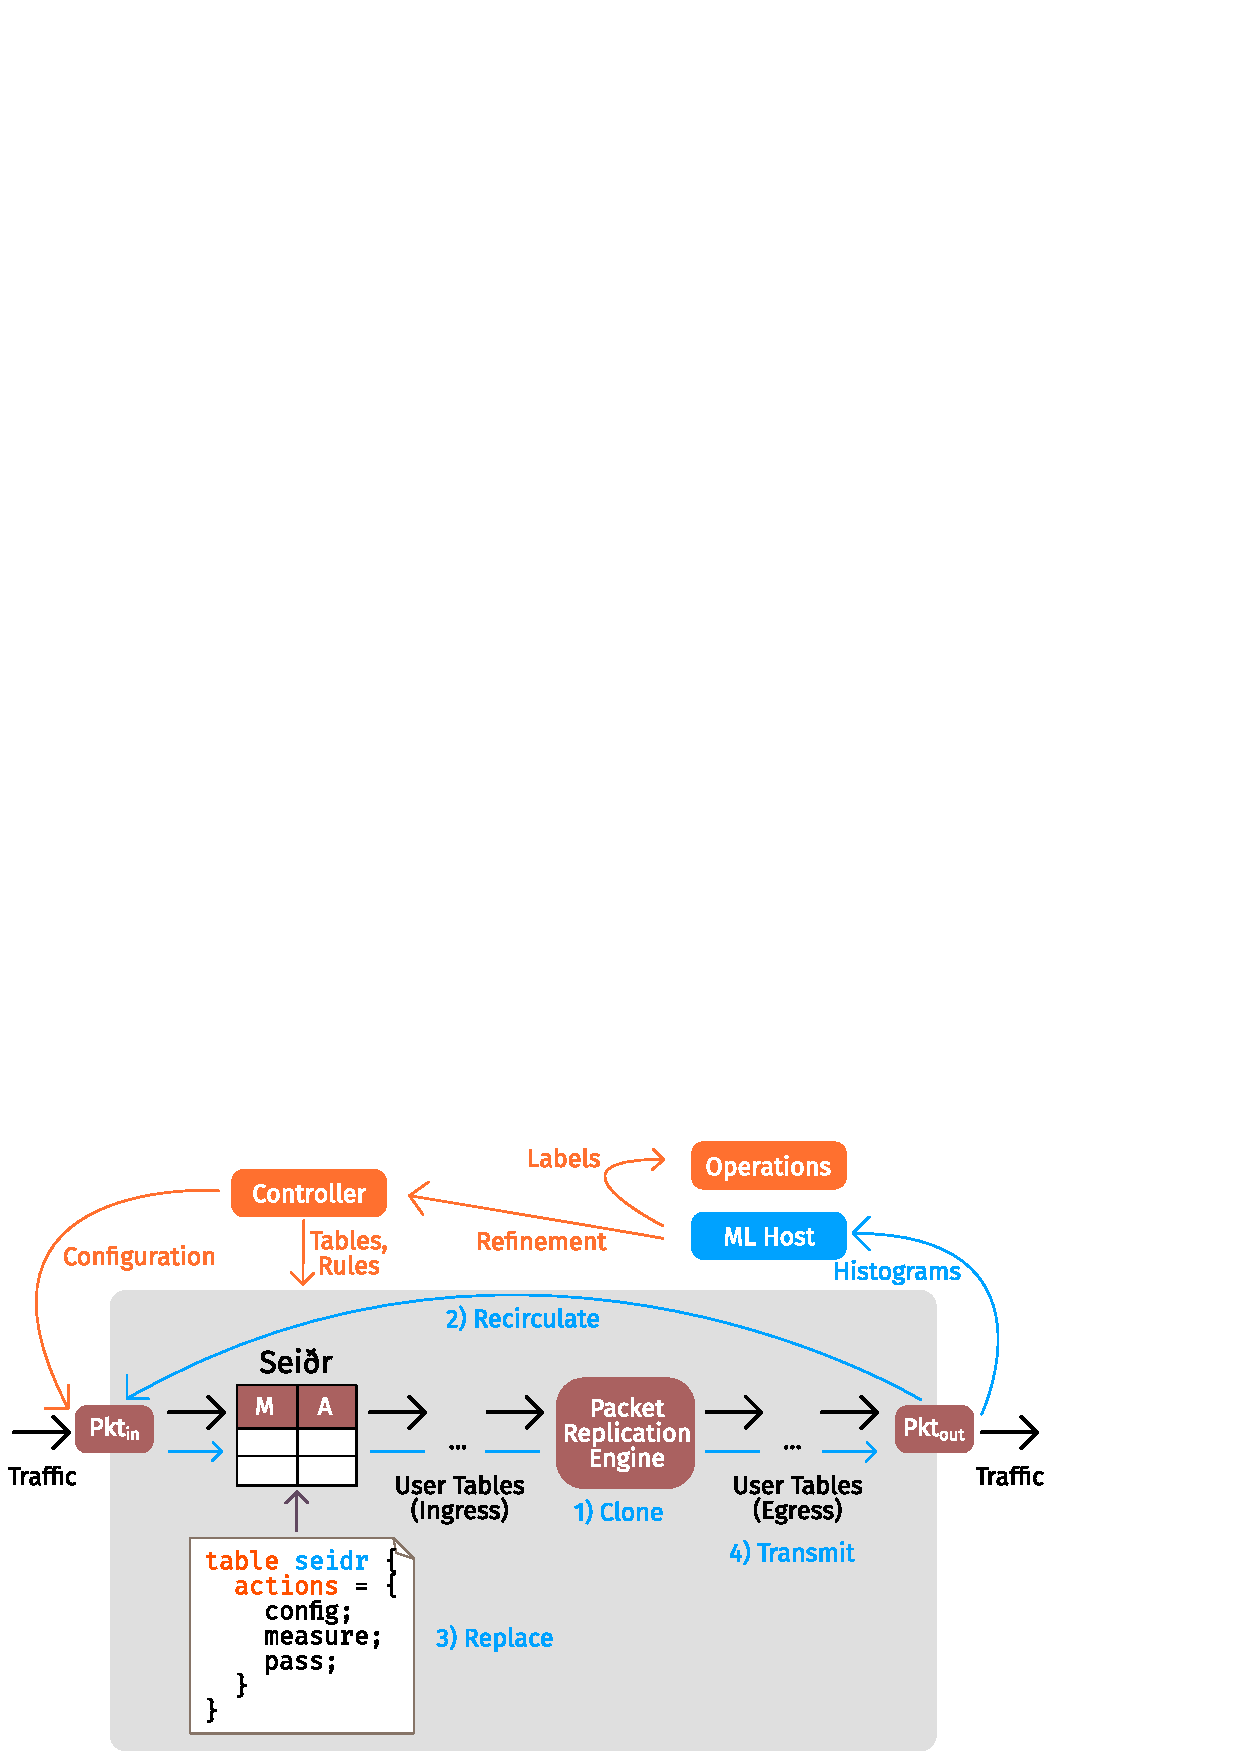
\includegraphics{diagrams/seidr/dp-arch-diagram.pdf}}
    \caption{\seidr{}'s integration with a PSA-compatible~\cite{p4-psa} dataplane.}
    \label{fig:arch}
\end{figure}

% Let's show them a histogram datastructure would look like purely with registers and how would a P4 action populate it - pseudocode or P4 snippet would be nice.

Although packet timing information is useful in understanding network and flow behaviour, without volume or packet rate reduction it is prohibitively expensive for hosts to handle each packet.
Histogramming acts as the \emph{aggregation step} which makes this class of analysis feasible in high-speed networks.
\Cref{fig:arch} demonstrates how \seidr{}, installed as an additional table in any P4 program, records and transmits inter-arrival time histograms.
The format for these histogram packets is outlined in \cref{fig:seidr-headers}; we choose to store individual buckets as \mintinline{rust}{u16}s, and the number of buckets in any histogram is fixed at compile time.
We set this to \num{100} buckets per histogram.
Packets traverse a table which requires \num{3} actions to be implemented:
\begin{enumerate}
    \item \mintinline{rust}{config} reads any matched packets as a \mintinline{rust}{seidr_cfg_t} of type \mintinline{rust}{SET_}\{ \mintinline{rust}{MIN}, \mintinline{rust}{MAX}, \mintinline{rust}{DST}, \mintinline{rust}{SRC}, \mintinline{rust}{LEN} \} by using the P4 parser.
    These update registers \numrange{1}{5} in \cref{tab:registers}, dropping any matched packets.
    
    \item \mintinline{rust}{measure} calculates the inter-arrival time, update per-flow histograms, and transmits finished histograms to the correct host. We describe its operation in \cref{alg:measure}.
    
    \item \mintinline{rust}{pass} ignores packets, and is the default action.
\end{enumerate}
Constructing \seidr{} in this manner allows the control plane to install rules to enable/disable runtime reconfiguration as needed, and to monitor as many or as few flows as desired (\ie, using wildcard rules, or exact matching).

The PSA does not have any mechanisms for generating new packets.
To circumvent this, any packet which would complete a histogram is tagged for cloning at the end of the ingress pipeline, and recirculation at egress (\cref{algline:recirc}).
This truncated copy returns to \seidr{}'s table, where we enable the relevant headers, change L2/3 fields, and write out the histogram contents (\crefrange{algline:rewrite-start}{algline:rewrite-end}).
The P4 deparser outputs the new protocol stack at egress, and transmits the histogram UDP packet into the network.
Event-driven architecture proposals~\cite{DBLP:conf/hotnets/IbanezABM19} may allow a more natural means of packet generation.

\begin{figure}
\centering
\begin{subfigure}{0.45\linewidth}
\centering
\adjustbox{max width = 0.6\linewidth}{
\begin{minipage}{\linewidth}
\begin{minted}[escapeinside=||]{rust}
|\textbf{\textcolor{Keyword}{header}}| seidr_cfg_t {
    bit<8> function;
    bit<144> payload;
}
\end{minted}
\end{minipage}
}
\end{subfigure}
\begin{subfigure}{0.45\linewidth}
\centering
\adjustbox{max width = 0.6\linewidth}{
\begin{minipage}{\linewidth}
\begin{minted}[escapeinside=||]{rust}
|\textbf{\textcolor{Keyword}{header}}| seidr_t {
    bit<128> src_ip;
    bit<128> dst_ip;
    bit<16> src_port;
    bit<16> dst_port;
    bit<16> eth_type;
    bit<BUCKETS * 16> histo;
}
\end{minted}
\end{minipage}
}
\end{subfigure}
\caption{P4 headers for \seidr{} configuration and histograms.}\label{fig:seidr-headers}
\end{figure}

\begin{algorithm}
% \vspace{-0.25cm}
% \DontPrintSemicolon
\KwData{5-tuple, P4 metadata, P4 headers, Registers}
h $\leftarrow$ hash(5-tuple)\;
index $\leftarrow$ BUCKETS * h\;
owner $\leftarrow$ HistoOwner[h]\;
\uIf{metadata.packet\_path = RECIRCULATE}{
    headers.tcp.valid $\leftarrow$ false\label{algline:rewrite-start}\;
    headers.udp.valid $\leftarrow$ true\;
    headers.seidr.valid $\leftarrow$ true\;
    copy 5-tuple into headers.seidr\;
    rewrite headers.ip, headers.udp using HistoSrc/Dest\;
    headers.seidr.histo $\leftarrow$ HistoData[index..]\;
    truncate payload\;
    zero out registers: BucketCount, HistoOwner[h], HistoData[index..]\;\label{algline:rewrite-end}
}
\ElseIf{owner = 0 \textbf{or} owner = 5-tuple}{\label{algline:owner-check}
    HistoOwner[h] $\leftarrow$ 5-tuple\;
    iat $\leftarrow$ LastTimestamp - metadata.mac\_ingress\_time\;
    \If{iat $\ge$ Min \textbf{and} iat $\le$ Max}{
        bucket $\leftarrow$ BUCKETS * (iat - Min) / (Max - Min)\;
        HistoData[index + bucket] $\leftarrow$ HistoData[index + bucket] + 1\;
        BucketCount[h] $\leftarrow$ BucketCount[h] + 1\;
        \If{BucketCount[h] = Len}{
            mark packet for cloning and recirculation\label{algline:recirc}\;
        }
    }
}

\caption{Histogram update and transmission.}\label{alg:measure}
\end{algorithm}

In the event of hash collision (\cref{algline:owner-check}), we ignore packets outside of the tracked flow to ensure that data is accurate.
As later processing and classification directly affect what decisions are made by operators or automatically taken by a policy (possibly leading to incorrect flow limits, QoS, \emph{etc.}), avoiding corruption/cross-contamination of operational data is paramount.
To gain collision resistance, Robin Hood hashing could be used up to a maximum distance in the table, treating a zeroed owner as empty and an illegal source IP as a tombstone value.

\begin{table}
    \centering
    \caption{Register map (Datatype, Amount) for an $h$-bit hash.}
    \resizebox{\linewidth}{!}{\begin{tabular}{@{}ccccccccc@{}}\toprule
        Min & Max & Length & HistoSrc & HistoDest & BucketCount & LastTimestamp & HistoOwner & HistoData \\ \midrule
        \mintinline{rust}{u16} & \mintinline{rust}{u16} & \mintinline{rust}{u16} & \mintinline{rust}{u16 + u128} & \mintinline{rust}{u16 + u128} & \mintinline{rust}{u16} & \mintinline{rust}{u64} & \mintinline{rust}{3 * u16 + 2 * u128} & \mintinline{rust}{BUCKETS * u16} \\
        1 & 1 & 1 & 1 & 1 & $2^h$ & $2^h$ & $2^h$ & $2^h$ \\ \bottomrule
    \end{tabular}}
    \label{tab:registers}
\end{table}

% Basic Logic:
% \begin{itemize}
%     \item table 1: three actions
%     \begin{itemize}
%         \item config: set R1 or R2 (controller installs rule matching a specific port/ip combo)
%         \item measure: take ingress timestamp from metadata, do stuff, write into lasttime, add to bucket and total if within bounds
%         \item pass (default)
%     \end{itemize}
%     \item then pass onto rest of tables
%     \item Why do it this way? can make it all or nothing through control plane.
%     \item How to write and send packet? Same trick as ESNET? (recirc w/ custom metadata to transform pkt)
% \end{itemize}

% ?? NOTE: See PSA \cite{p4-psa} for register format. Some papers, like Dapper, suggest that hash tables should be possible? That would work out very well in our benefit.

% ?? What is configurable? Min, max of the histogramming range

This design allows runtime configuration of all aspects save for the bucket count; at runtime, the only way to increase bucket resolution is to examine a smaller region of IATs.
While in theory this could be configured below a maximum compiled into the firmware, the difficulties introduced in classification/data processing make this infeasible.
Unless using stream-capable classifiers such as LSTMs~\cite{DBLP:journals/neco/HochreiterS97}, changing the input size requires retraining from scratch since new neuron weights must be added and structural properties of the input data change.
Increasing the bucket count requires new firmware installation, as many dataplane P4 implementations cannot allocate variable-length stores due to the lack of a dynamic allocator.

\begin{figure}[t]
    \centering
    \begin{subfigure}[t]{0.49\linewidth}
        \centering
        \resizebox{\linewidth}{!}{\includegraphics{plots/seidr/dt-cubic-1000-app.pdf}}
        \subcaption{TCP Cubic}
        \label{fig:cubic-hist-app}
    \end{subfigure}
    \begin{subfigure}[t]{0.49\linewidth}
        \centering
        \resizebox{\linewidth}{!}{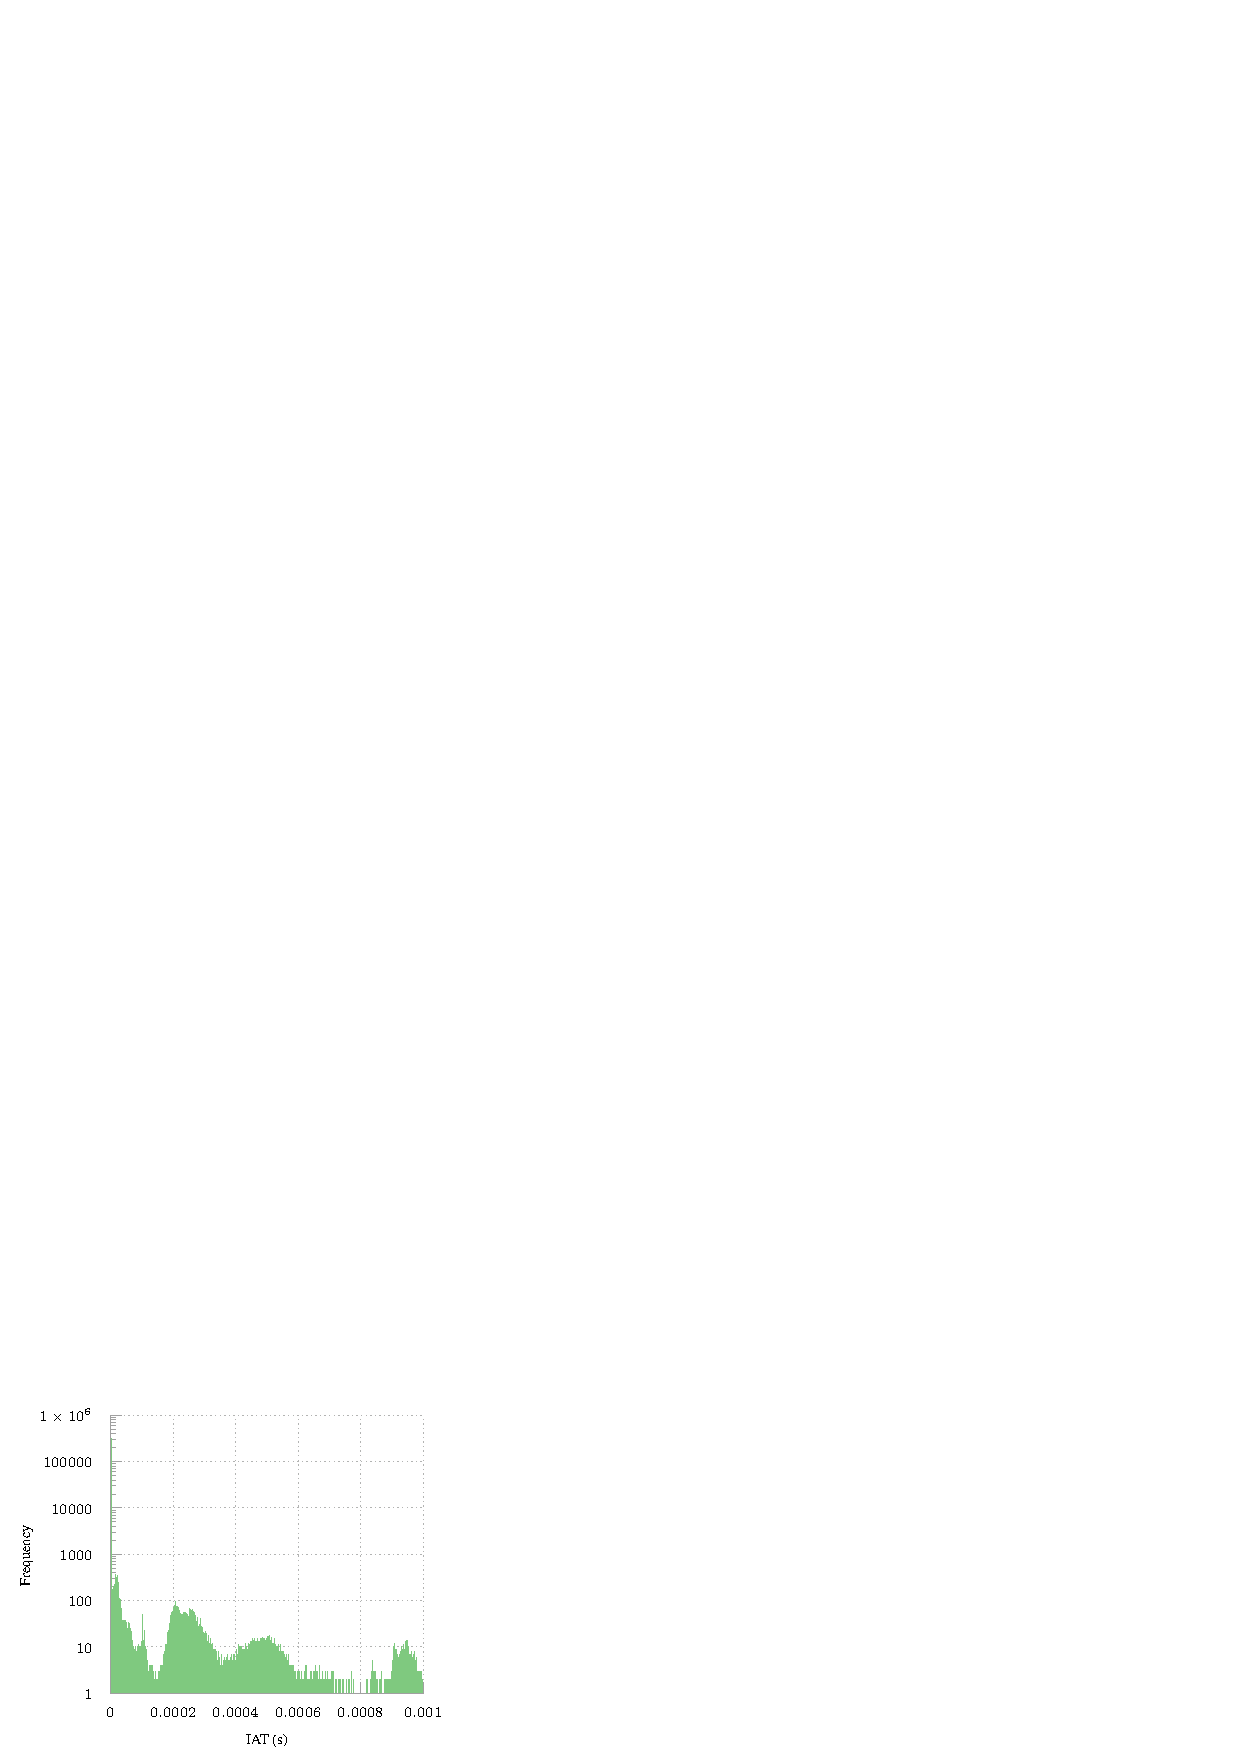
\includegraphics{plots/seidr/dt-bbr-1000-app.pdf}}
        \subcaption{TCP BBR}
        \label{fig:bbr-hist-app}
    \end{subfigure}
    \caption{Example dataplane histograms showing visible differences in inter-arrival times of selected TCP flavours. Our ML solutions are trained to programmatically identify such differences.}
    \label{fig:tcp-hist-app}
\end{figure}

As an example of dataplane-generated histograms, \cref{fig:tcp-hist-app} shows the distribution of inter-arrival times between two TCP congestion control algorithms. The visible differences are programmatically identified using our ML algorithms.

\subsection{Accurate, Precise and High-Resolution Timestamping}

Precise timestamps are critical when detecting temporal properties of flow behaviour, such as microbursts or inferring flow congestion control algorithms.
It is especially important in high speed (\SI{100}{\giga\bit\per\second}) networks, where there can be as little as \SI{6.7}{\nano\second} between packets that need to be analysed.
With a Linux-based software solution (\eg, reading packets from a link with \emph{tcpdump}), the Linux kernel can only provide microsecond-level accuracy with precision in the order of \SI{100}{\micro\second}~\cite{kundel2020p4sta}.
DPDK improves on this, increasing the accuracy to \SI{100}{\nano\second} in the best case~\cite{primorac2017measure}.
However, today's dataplane devices (\eg, Netronome SmartNICs, NetFPGA SUME) allow nanosecond-accurate timestamps to be retrieved from the \emph{Media Access Control} (MAC) modules with a precision of \SI{10}{\nano\second}~\cite{kundel2020p4sta}, a timestamp property \seidr{} relies upon.

% Some platforms provide picosecond-level precision and many solutions allow time synchronisation between multiple devices using the IEEE 1588-2002 (Precision Time Protocol) standard.



\section{TCP congestion control classification}\label{sec:seidr-tcpcc}


% We present an example of first-stage analysis performed for each flow and each packet---stateful TCP analysis.
% This includes numerous metrics which are considered standard when measured at connection endpoints, yet are difficult or invite numerous issues when performed in the network (of which we include a discussion on drawbacks and, curiously, benefits).
% The introduction of accurate timestamps allows us to explore rate-monitoring at a per-packet level, a new view of flow behaviour which may enable flow and hardware characterisation.

% \subsection{Per-Packet Rate Monitoring}

% \begin{figure*}
%     \centering
%     \begin{subfigure}[t]{0.49\linewidth}
%         \centering
%         \resizebox{0.5\linewidth}{!}{
% 	    \begin{tikzpicture}
%     		[packet/.style={draw, fill=uofgsunshine}]
% 		    \node[packet] (p1) {$p_1$: 1500B};
% 		    \node[packet, right= 1cm of p1] (p2) {$p_2$: 800B};
		
% 		    \node at ($(p1.south west) - (0,1)$) (t1) {$t_1$};
% 		    \node at ($(p2.south west) - (0,1)$) (t2) {$t_2$};
		
% 		    \draw[-, dotted] (t1.north)--(p1.south west);
% 		    \draw[-, dotted] (t2.north)--(p2.south west);
		
%     		\draw[<->] (t1.north) -- node[below]{$\mathit{dt}$} (t2.north);
% 	    	\draw[<->] ($(t1.north) + (0,0.2)$) -- node[above]{$s$} ($(t1.north) + (1.8,0.2)$);
% 		    \draw[<->] ($(t1.north) + (1.8,0.2)$) -- node[above]{$g$} ($(t2.north) + (0,0.2)$);
% 	    \end{tikzpicture} 
% 	}
%     \caption{\centering Per-packet rate, visualised. Note that $p_1$ and $p_2$ are not necessarily packets from the same flow.}
%     \label{fig:per-packet-rate}
%     \end{subfigure}
%     \begin{subfigure}[t]{0.49\linewidth}
%     \centering
%     \resizebox{0.9\linewidth}{!}{
% 		\begin{tikzpicture}
% 		[packet/.style={draw, fill=uofgsunshine}]
% 		\node[packet] (p1) {$p_1$: 1500B};
% 		\node[packet, right= 1cm of p1] (p2) {$p_2$: 800B};
% 		\node[right= 1cm of p2] (p3) {...};
% 		\node[packet, right= 1cm of p3] (p4) {$p_{n-1}$: 1500B};
% 		\node[packet, right= 1cm of p4] (p5) {$p_n$: 1500B};
		
% 		\node at ($(p1.south west) - (0,1)$) (t1) {$t_1$};
% 		\node at ($(p2.south west) - (0,1)$) (t2) {$t_2$};
% 		\node at ($(p4.south west) - (0,1)$) (t4) {$t_{n-1}$};
% 		\node at ($(p5.south west) - (0,1)$) (t5) {$t_{n}$};
		
% 		\draw[-, dotted] (t1.north)--(p1.south west);
% 		\draw[-, dotted] (t2.north)--(p2.south west);
% 		\draw[-, dotted] (t4.north)--(p4.south west);
% 		\draw[-, dotted] (t5.north)--(p5.south west);

%         \draw[<->] ($(t2.south) + (0,-0.25)$) -- node[above]{$s$} ($(t2.south) + (6.25,-0.25)$);
%         \draw[<->] ($(t2.south) + (6.25,-0.25)$) -- node[above]{$g$} ($(t5.south) + (0,-0.25)$);
% 		\draw[-, thick] ($(t2.south) - (0,0.5)$) -- node[below]{$W$} ($(t5.south) - (0,0.5)$);
% 		\end{tikzpicture} 
% 	}
%     \caption{\centering Sliding window rate, visualised. Rate estimates are computed using the sizes of the last $W$ packets seen in the current flow. Packets $p_2$ and $p_{n-1}$ belong to the same flow, but $p_n$ is not assumed to.}
%     \label{fig:sliding-window-rate}
%     \end{subfigure}
%     \caption{Comparison of per-packet and sliding window rates. The lengths of packets and inter-packet gaps are not to scale, and are purely demonstrative.}
%     \label{fig:pr-vs-slide}
% \end{figure*}

% Associating each packet with a high-resolution timestamp allows us to introduce the notion of a \emph{per-packet rate}.
% Assuming a packet with size $p$ arrives at time $t_1$ and is followed by another packet (potentially from another flow) which arrives at $t_2$, we measure $\mathit{dt}=t_2-t_1$ for this packet.
% Supposing this first packet spends time $s$ on the wire and assuming that the inter-packet gap $g$ is negligible compared to the length of a packet, then $\mathit{s} = \mathit{dt} - g \approx \mathit{dt}$.
% This packet then has a point rate, $r$:
% \begin{equation}
%     r = \frac{p}{s} \approx \frac{p}{\mathit{dt}}
% \end{equation}
% \Cref{fig:pr-vs-slide} demonstrates how this timing information arises, contrasted with sliding-window rate measurements taken over a longer time period.
% This assumes almost back-to-back traffic, which is realistic in our deployment environment, but to the best of our knowledge no programmable switches expose the timestamp at which the final bit of a packet has been ingested.
% Such a timestamp would allow exact measurement of $s$.

% % ?? we need to be clear about the unintuitive nature of these measurements, include a quick sketch proof which shows that the weighted average of a set of point rates is analytically identical to the sliding window rate/throughput taken over the same period of time.
% While this is an interesting measure to associate with each packet, considering how best to view such rates in aggregate can be counter-intuitive.
% Viewing these rates as time series data reveals interesting distributional characteristics which disagree starkly with our understanding of a flow's rate---for instance, clusters which suggest a different mean.
% Suppose we have a set of measurement indices $C$ with no gaps captured between $t$ and $t'$, partitioned into flows $C = F_1 \cup \dots \cup F_p$.
% To correctly combine a set of point measurements for a flow $F_i$ into an average rate $\overline{r}_{F_i}$, we compute:
% \begin{equation}
%     \overline{r}_{F_i} = \frac{\sum_{a \in F_i} \mathit{dt}_a r_a}{\sum_{c \in C} \mathit{dt}_c}.
% \end{equation}
% In the instance that only one flow is captured (\emph{i.e.}, $F_i = C$), this is a weighted average over point rates, using the $\mathit{dt}$ measured between each packet and the next packet in the same flow as its weight.
% Similarly, this is analytically equivalent to the sliding-window rate measured over the same set of packets:
% \begin{equation}
%     \frac{\sum_{a \in F_i} \mathit{dt}_a r_a}{\sum_{a \in F_i} \mathit{dt}_a} \simeq \frac{\sum_{a \in F_i} p_a}{t' - t}.
% \end{equation}
% % \begin{proof}
% % Given a set of contiguous measurements from the same flow $S \subseteq \mathbb{Z}$, admitting $p_s$, $r_s$, $\mathit{IAT}_s$ and $t_s$, the weighted average of point rates is then
% % $$
% % \overline{r}_S = \frac{\sum_{s \in S} \mathit{IAT}_s r_s}{\sum_{s \in S} \mathit{IAT}_s}
% % $$
% % The sliding-window average:
% % $$
% % \overline{r}_S = \frac{\sum_{s \in S} \mathit{IAT}_s r_s}{\sum_{s \in S} \mathit{IAT}_s}
% % $$
% % \end{proof}

% We assume that inter-packet gaps will be negligible (\emph{i.e.}, that the link is never in a state of very low utilisation), due to typically high utilisation on a WAN.
% % Similarly, we need to discuss the effects of selective monitoring or an abundance of UDP/ICMP traffic (which will distort $dt$s).
% However, this assumption can be distorted if selective TCP flow monitoring is used, or if UDP/ICMP traffic is overabundant; both these scenarios create larger gaps between TCP packets of interest, inflating $g$ to the point where it is comparable in size to $s$.
% This has an impact on our notion of per-packet rates, but not inter-arrival times or other such dependent metrics.
% The effect is small on sliding window rates, particularly at larger window sizes.
% ?? Justify. On paper, it looked like error term was O(1/n), O(g) for an n packet window.


% \section{Inter-Arrival Time}

% Having assigned each packet in a flow with a nanosecond-accurate timestamp ?? tbc

\Cref{fig:tcp-hist-app} suggests that a notable use-case for this type of measurement is \emph{congestion control algorithm} (CCA) detection.
In a TCP connection, each machine is free to choose the CCA it uses to send bytes, and thus how it responds to network congestion signals.
This choice is local, and so is invisible to the other machine (and the network).
In datacentre networks, operators choose these to ensure optimal behaviour.
In a transit network or large WAN however, these hosts (and thus the CCAs in use) are outside the control of network operators, which introduces difficulties when CCA interactions lead to \emph{unfairness}.
Consider the recent (and widespread) introduction of \emph{TCP BBR}~\parencite{DBLP:journals/queue/CardwellCGYJ16}.
\emph{BBR} is a delay/model-based CCA which converges on a fair share of bottleneck bandwidth by reducing its rate if the round-trip time increases, while periodically attempting to increase send rate to account for path/load changes.
However, \emph{BBR} traffic can consume \SI{40}{\percent} of link capacity when multiplexed with loss-based CCAs, regardless of the number of competing flows~\parencite{DBLP:conf/imc/WareMSS19}. 
When ensuring fair transit to all flows, this is hardly a desirable outcome; in fact, it's one which may frustrate clients or violate SLAs.

A curious property of \emph{BBR}'s algorithm which sets it apart from other variants is that packet transmission is \emph{timer-based}.
\texttt{send(packet)}, as defined in the canonical algorithm, asks that on transmission of a packet, the sender should wait for the estimated time that packet would take to reach the recipient.
For instance, at an estimated bottleneck bandwidth of \SI{8}{\mega\bit\per\second}, a \SI{1024}{\kilo\byte} packet would hold back the next packet in the flow until \SI{976.6}{\micro\second} had elapsed.
When packet sizes remain similar this causes strongly periodic behaviour, while mode switches in the \emph{BBR} algorithm cause these periodic bands to shift up or down accordingly.
This effect is stronger than in existing loss- and delay-based algorithms which remain intrinsically tied to the notion of a congestion window (where release of buffered packets follows the receipt of ACK messages).
As a result, timing behaviour of past CCAs may be influenced by (the lack of) packet pacing, periodic components might be made noisier by jitter along the return path, or the behaviour of the receiver might add further noise.

This high-level analysis of \emph{BBR} gives us a strong feature to use as the basis for classification: the \emph{inter-arrival times} (IATs) for each packet in a flow.
We have two options for processing this for classification: we may use a compressed, fixed-size representation such as histograms to capture the aggregate distribution, or we may attempt to capture structural behaviour by using a variable-length stream of IATs.
In many networks, the data and packet rate reduction offered by the former is required to make this possible.
Indeed, in-switch aggregation has seen great success in aiding ML for training~\parencite{DBLP:conf/isca/LiLYCSH19}, and direct execution~\parencite{DBLP:conf/hotnets/XiongZ19}.
We make use of the following standard classification algorithms on a fixed-size representation to attempt to single out the CCA in use:

\begin{itemize}
    \item \emph{$k$-Nearest Neighbours ($k$-NN)}. A simple and well-understood classifier which assigns labels based on the closest members of the training corpus (\ie, by the $L_2$ metric). Linear memory cost in amount of training data, and no training cost other than loading all data points, but capable of learning complex decision boundaries on fixed-length input.
    
    \item \emph{Convolutional Neural Networks (CNNs)}. A neural network approach which learns convolution kernels to classify fixed-length data, particularly when recognising spatial features. Memory cost is fixed for a given architecture irrespective of training data, with a high training cost.
\end{itemize}
% \fakepara{Long Short-Term Memory~\parencite{DBLP:journals/neco/HochreiterS97} units (LSTMs)} A class of recurrent neural network used for stream classification, forecasting, and prediction of variable-length data. Memory cost is fixed, with longer training times (and more data required) than similarly sized CNNs.
% Of these, we apply $k$-NN and CNNs to histograms of packet IATs, and LSTMS to raw IAT streams.

When examining $k$-NN classifiers, we measured accuracy across choices of $k \in \left[2, 8\right]$.
We found $k=2$ to be the most effective choice with our input data using the $L_2$ metric.
Our CNN architecture is described in \cref{tab:cnn-arch}, using ReLu activation and $1 \times 1$ stride in convolutional layers unless stated otherwise.
Training occurred over 5 epochs using the Adam optimiser with categorical cross-entropy as a loss metric, and a batch size of \num{64} histograms (\num{8} for full sequences due to the smaller data volume).
For \emph{BBR vs.\ Cubic}, the complete model consists of \num{104898} 32-bit floating-point parameters (\SI{409.76}{\kibi\byte}), while the full classification task adds a further \num{130} parameters (\SI{0.51}{\kibi\byte}).

\begin{table}
    \centering
    \caption{CNN architecture for \num{100}-entry histograms.}
    \resizebox{0.7\linewidth}{!}{\begin{tabular}{@{}cccc@{}}\toprule
        Layer & Nodes/Filters & Filter Size & Output Dimension \\ \midrule
        Conv2D & 32 & $(3 \times 1)$ & $(98 \times 1 \times 32)$ \\
        MaxPool & --- & $(2 \times 1)$ & $(49 \times 1 \times 32)$ \\
        Conv2D & 64 & $(3 \times 1)$ & $(47 \times 1 \times 64)$ \\
        MaxPool & --- & $(2 \times 1)$ & $(23 \times 1 \times 64)$ \\
        Conv2D & 64 & $(3 \times 1)$ & $(21 \times 1 \times 64)$ \\
        Flatten & --- & --- & \num{1344} \\
        Dense & 64 & --- & \num{64} \\
        Dense (Softmax) & $n_\mathit{classes}$ & --- & $n_\mathit{classes}$ \\
        \bottomrule
    \end{tabular}}
    \label{tab:cnn-arch}
\end{table}


\section{Evaluation}\label{sec:seidr-evaluation}
%Traffic is played back from hosts via Tcpreplay at a bandwidth assigned uniformly from a `good' or `bad' distribution, each using the same pcap file with source and destination IP addresses rewritten.

This work is most naturally compared against Marl, introduced by \textcite{DBLP:journals/eaai/MalialisK15}, the state-of-the-art in \gls{acr:rl}-based \gls{acr:ddos} prevention.
We are most interested in seeing how their approach contrasts with the new agent designs across different topologies and workloads.
Different network environments will also impose different levels of host density, where popular web servers may have orders of magnitude more clients than egress points from their network---I aim to show how these characteristics affect performance and learning rate.
Marl is known to outperform the AIMD~\parencite{DBLP:journals/ton/YauLLY05} strategy, yet the state of the art has long since moved on.
To paint a more current picture, I compare this work against an effective modern approach, \emph{SPIFFY}~\parencite{DBLP:conf/ndss/KangGS16}.
SPIFFY tests a proportion of flows by routing them through an alternate path with higher bandwidth, observing how their speed changes some time later.
This comparison lets us position our new agent designs against the state of the art, observing that SPIFFY has a similar mode of interaction to \gls{acr:rl}-based systems (taking action, observing an effect, and acting once again) and does not rely on protocol characteristics or signatures.
In reimplementing SPIFFY, I make the simplifying assumption that a suitable unused path exists (with identical bandwidth to the server's link).
\qty{10}{\percent} of active flows were tested at a time (according to the authors' observation that there is a factor of \qty{10}{\times} difference between the ideal and achieved bandwidth expansion), excluding flows below \qty{50}{\kilo\bit\per\second} and requiring a \qty{3}{\times} expansion from legitimate flows, making a judgement after \qty{5}{\second}.

To test this, I made use of both traffic models introduced in \cref{sec:a-new-normal} (Opus and \gls{acr:tcp}), both topologies discussed below (1-dest vs.\ Fat-Tree), and vary the amount of hosts typically communicating over each agent's ingress/egress node.
Additionally, these new models were evaluated in multi-agent mode (\emph{separate}, no model sharing), and in single-agent mode (\emph{single}, zero-cost perfect information sharing).
In each case, the algorithm's performance was averaged over \num{10} episodes of length \num{10000} timesteps (setting each agent's $\wvec{}=\mathbf{0}$ between episodes).
Host allocations at the beginning of each episode were generated pseudorandomly to ensure fairness between episodes---a host is malicious with probability $\operatorname{P}\left(\mathit{malicious}\right)$, and is benign otherwise.
Benign hosts generate traffic according to either \cref{sec:tcp-http-traffic-model,sec:udp-opus-traffic-model} depending on the experiment, while malicious hosts generate traffic as described in \cref{sec:attack-traffic-model} (both at experiment-dependent rates).

All experiments were executed on Ubuntu 18.04.2 LTS (GNU/Linux 4.4.3-040403-generic x86\_64), using an Intel Core i7-6700K (\qtyproduct[product-units=single]{4 x 4.2}{\giga\hertz}) which had \SI{32}{\gibi\byte} of \gls{acr:ram}.
%All code underpinning these findings is available on a public repository\footnote{\url{https://github.com/FelixMcFelix/rln-dc-ddos-paper}}.
%All code underpinning these findings is available on a public repository.\footnote{Private until publication.}

\subsection{Single destination}\label{sec:single-dest}
%?? Move description of tree topol to here.
The network is tree-structured, where one server $s$ connects through a dedicated switch to $k$ team leader switches, each connected to $\ell$ intermediate switches, which in turn each connect to $m$ egress switches.
We then have $N_{\mathit{hosts}} = k \ell m n$.
\Cref{fig:marl-topol} demonstrates this.
%Although \citeauthor{DBLP:journals/ccr/MahajanBFIPS02a}, the originators of this topology, make it clear that it exists as a fairly unrepresentative example \cite{DBLP:journals/ccr/MahajanBFIPS02a}, it remains the case that such a network topology allows for functional testing, and indeed is illustrative of one way in which attack traffic might aggregate in the network.
%It is hard, however, to argue its relevance to specific classes of victim or to reason about the interactions it might have with dependent applications.
%We aim to address this through \cref{sec:performance-in-an-emulated-environment}.
The network topology was configured using $k=2$ teams, $\ell=3$ intermediate nodes per team, $m=2$ agents per intermediate node, and $n \in \{2, 4, 8, 16\}$ hosts per learner.
This is a slight simplification of \Textcite{DBLP:journals/eaai/MalialisK15}'s \textquote{online} experiment, choosing fewer teams but remaining as a single server with a fan-out network.
%The algorithm parameters were set at $\gamma=0$ (leading to opportunistic behaviour), $\alpha=0.05$, having linearly annealed $\epsilon=0.2 \rightarrow 0$ by $t=3000$.
%Benign and malicious hosts uploaded between \SIrange{0}{1}{\mega\bit\per\second} and \SIrange{2.5}{6}{\mega\bit\per\second} respectively, and hosts were redrawn at each episode's start with $\operatorname{P}(\mathit{malicious})=0.4$.
%$U_s$  $k \ell mn+2$ \si{\mega\bit\per\second}.
%The performance of each choice of $n$ was averaged over \num{10} episodes of length \num{10000} timesteps (setting each agent's $\wvec{}=\bm{0}$ between episodes).
%Host allocations were generated pseudorandomly to ensure fairness between choices of $n$.
%These parameter choices match those of the original study to enable direct comparison, and are (to the best of our knowledge) arbitrary, but we justify our range of $n$ as capturing increasing scales of host activity.

\begin{figure}
	\centering
	\resizebox{0.9\linewidth}{!}{\begin{tikzpicture}[
	texts/.style = {text=black},
	labeltexts/.style = {text=uofgsandstone},
	treeline/.style = {draw=uofgburgundy},
	treenode/.style = {texts, circle, centered, fill=white, treeline},
	load/.style = {fill=uofgcobalt},
	loadhide/.style = {fill=uofgcobalt!40!white},
	external/.style = {fill=uofgrust},
	externalhide/.style = {fill=uofgrust!40!white},
	hideline/.style = {draw=uofgsandstone!40!white},
	hidenode/.style = {treenode, hideline},
	grow'=right
]
	\node[treenode, label={[texts]above:Server}] (root) {}
	child [treeline] { node [treenode, label={[texts]above:Core}] (sswitch) {}
		child [treeline] { node [treenode, label={[texts]above:Leader}] (teaml) {} 
			child [treeline] { node [treenode, label={[texts]above:Intermediate}] (inter) {}
				child [treeline] { node [treenode, load, label={[texts]above:Agent/Egress}] (agent) {}
					child [treeline] { node [treenode, external] (extern) {}
						child [treeline] { node [treenode, external, label={[texts]above:Host}] (host) {} }
						child [hideline] { node [hidenode, externalhide] (endhost) {} }
					}
				}
				child [hideline] { node [hidenode, loadhide] (endagent) {} }
			}
			child [hideline] { node [hidenode] (endinter) {} }
		}
		child [hideline] { node [hidenode] (endteaml) {} }
		edge from parent
		node[below, labeltexts] {$U_s$}
	};
	
	%\draw[-] (teaml) -- (endteaml);
	\node [labeltexts] (kdots) at ($(teaml)!0.5!(endteaml)$) {$\rvdots$};
	\node [labeltexts, right = -0.1cm of kdots] {$k$};
	\node [labeltexts] (ldots) at ($(inter)!0.5!(endinter)$) {$\rvdots$};
	\node [labeltexts, right = -0.1cm of ldots] {$\ell$};
	\node [labeltexts] (mdots) at ($(agent)!0.5!(endagent)$) {$\rvdots$};
	\node [labeltexts, right = -0.1cm of mdots] {$m$};
	\node [labeltexts] (ndots) at ($(host)!0.5!(endhost)$) {$\rvdots$};
	\node [labeltexts, right = -0.1cm of ndots] {$n$};
\end{tikzpicture}}
	\caption[Tree-structured network topology diagram for evaluating a single-destination network.]{
		Network topology diagram, showing how the server and its core switch's $k$ teams are structured, with $\ell$ intermediate routers per team, connected to $m$ agents which each moderate $n$ hosts beyond a single external switch.
		%	Empty nodes are considered to be internal.
		Red nodes are external, and each blue node hosts an agent.
		\label{fig:marl-topol}
	}
\end{figure}

\subsection{Multiple destinations}
The previous topology allows for direct comparison against the state-of-the-art, and indeed is illustrative of one way in which attack traffic might aggregate in the network.
It is hard, however, to argue its relevance to specific classes of victim or to reason about the interactions it might have with dependent applications.
In contrast, the fat-tree topology~\parencite{DBLP:conf/sigcomm/Al-FaresLV08} sees regular use in real-world data centres and scales well horizontally.
%?? Come up with description of fat-tree (multi-dest) topol.
%?? Why fat tree? regularly appears in modern datacentres.
%?? $k=4$ fat-tree , with one pod hosting two servers $s_0,s_1$.
We use a $k=4$ fat-tree, with one pod hosting two servers $s_0$ and $s_1$.
$n$ external hosts connect through each core switch (where agents are hosted), and communicate with $s_0, s_1$ uniformly randomly.
Both servers host identical services.
We set $n \in \{6, 12, 24, 48\}$ hosts per learner (keeping $N_{\mathit{hosts}}$ identical to each tier of the single-host topology), and restrict $U_{s_0} = U_{s_1} = U_s / 2$.

\subsection{Parameters}
The algorithm parameters were set at $\alpha=0.05$, linearly annealing $\epsilon=$ \num{0.2} $\rightarrow$ 0 by $t=$~\num{3000} in the case of Marl (\num{8000} actions per agent in the \emph{Instant/Guarded} models).

Benign hosts each occupied \qtyrange{0}{1}{\mega\bit\per\second}, and hosts were redrawn at each episode's start with $\operatorname{P}(\mathit{malicious})=$~\num{0.4}.
%The original introduction of this approach to direct-control reinforcement learning as introduced by \textcite{DBLP:journals/eaai/MalialisK15} fails to consider key cases: the absence of a suitable heuristic classifier $g(\cdot)$, disjoint ranges of traffic distribution (i.e., the presence of benign heavy-hitters), the accurate simulation of TCP-like behaviour (and its effects on collateral damage), and high densities of hosts at egress points.
%?? Why? ...
%Of these, the latter two are most deserving of a closer investigation, as they have stronger implications for wide-scale deployment.
%These are important issues, particularly when we consider real-world deployment.
%Heuristic estimates of traffic legitimacy come with computational cost and couple the reward function to the accuracy of the estimator, hosts often show diversity in their own traffic patterns (perhaps being multi-modal), and it is known that TCP is the most used transport protocol for Internet traffic \cite{DBLP:conf/saint/ZhangDJC09}.
%?? NEED TO VERIFY VOLUME OF CONGESTION-AWARE PROTOCOLS
Malicious hosts each sent \qtyrange{2.5}{6}{\mega\bit\per\second} when attacking \gls{acr:udp} traffic, though this was increased to \qtyrange{4}{7}{\mega\bit\per\second} when using \gls{acr:tcp}-like traffic (to meaningfully impact benign flows).
Given $n$ and $\operatorname{P}(\mathit{malicious})$, we see an expected malicious bandwidth \numrange{1.27}{1.87} and \qtyrange{2.03}{2.18}{\times} $U_s$ respectively.
%The expected fraction of $U_s$ consumed by each host is \SI{21.5}{\percent} for $n=2$, and \SI{2.84}{\percent} for $n=16$.
For these choices of $n$ in both topologies, we observe $N_{\mathit{hosts}} \in \left\{24, 48, 96, 192\right\}$, and an expected number of malicious hosts $\mathbb{E}\left[N_{\mathit{attackers}}\right] \in \left\{9.6, 19.2, 38.4, 76.8\right\}$.
For the largest choice of $n$, we see an expected total attack traffic $\mathbb{E}\left[V_{\mathit{attack}}\right] =$ \qtylist{334.05;422.4}{\mega\bit\per\second} for Opus and \gls{acr:http} traffic respectively.

$U_s$ was fixed at $N_{\mathit{hosts}}+2$ \unit{\mega\bit\per\second} (to account for burstiness), and each link had a delay of \qty{10}{\milli\second}.
All links had unbounded capacity, save for each server-switch.
These parameters match those of the original study to enable direct comparison, and many are (to the best of our knowledge) arbitrary, but I justify the range of $n$ as capturing increasing scales of host activity.

% \section{Related Work}\label{sec:related}
% %?? Try and compare my work here when possible?

\fakepara{DDoS Prevention}
\Textcite{DBLP:conf/lcn/BragaMP10} examine the detection of flooding DDoS attacks through \emph{self-organising maps}, using SDN to gather statistics effectively.
Many of their features aren't overly relevant, as their focus is not active defence or discovering \emph{which} hosts contribute to an attack.
%?? Actually talk about Marl (???) to appease reviewer \#1.
The closest available approach within this field is that of \textcite{DBLP:journals/eaai/MalialisK15} (whom we have positioned our work against), and their contribution in applying RL to the task of intrusion prevention is significant: their work helps to show the viability of live, adaptive, feedback-loop-like control of the network to detect and prevent DDoS attacks.
They create a tree overlay topology (subdivided into teams), where each agent applies packet drop to \emph{all} flows inbound to a protected server.
%?? Recap their flaws, since they've been cut form every other aspect.
Our results show that their technique underperforms at high host density and when congestion-aware traffic dominates---that their results do not demonstrate this suggests an evaluation driven purely by traces (rather than live application dynamics).

\emph{SPIFFY} \cite{DBLP:conf/ndss/KangGS16} aims to remedy transit-link attacks by observing how flows from each source respond to a sudden increase in available bandwidth.
\Citeauthor{DBLP:conf/ndss/KangGS16} realise that bots participating in an attack are often unable to match this bandwidth expansion (having already saturated the capacity of their outbound links), while legitimate flows typically speed up to match the new fair-share rate.
%Attackers must either be detected or reduce the throughput of each bot, increasing the cost of launching an attack.
%Unlike our approach (and due to the class of attacks it is designed to defend against), SPIFFY is intended to be deployed within ASes, although .
A weakness of their approach is that computing a route to measure bandwidth expansion on real networks can be costly (up to \SI{14}{\second} for the Cogent topology), and that the low expansion factors in real network can require more ``rounds'' of filtering.
By contrast, our approach takes a constant time to compute an action for a flow regardless of topology size.
Their assumptions about traffic response to such bandwidth expansion do not hold for constant bitrate flows (e.g., VoIP) and may not extend to HTTP DASH flows, both of which make up a sizeable proportion of network traffic.

\emph{Athena} \cite{DBLP:conf/dsn/LeeKSPY17} is a generalised SDN framework for intrusion detection, but has shown the use of a \emph{k-nearest neighbours} classifier to detect individual attack flows.
Although heavyweight (and proven to be effective compared with \textcite{DBLP:conf/lcn/BragaMP10}), their comparison against SPIFFY lacks the quantitative evidence required to understand how the system compares.
\Textcite{DBLP:conf/sp/SmithS18} use AS-level routing to tackle both transit-link and flooding-based attacks.
This view is taken due to the perceived cost of per-stream classification and inherent sensitivity to adversarial examples.
The approach is creative, relying upon BGP \emph{fraudulent route reverse poisoning} to preserve traffic to a target AS, but unlike SPIFFY the approach doesn't actually \emph{remove} the congestion.
Because of this, flooding-based attacks aren't fully alleviated.

%?? Abuses of RL 
\fakepara{RL in Networks}
Earnest, well-considered application of RL towards the challenge of intrusion prevention has seen comparatively little examination.
Past work treats the paradigm as a traditional classifier for anomaly detection \cite{shamshirband2014anomaly} and DDoS prevention \cite{DBLP:conf/mates/ServinK08}.
Given that the main strengths of RL techniques are the ability to control ongoing interaction and adapt by observing the concrete effects of actions, such works don't apply the rich literature on the subject to its fullest potential.

For categorising how RL fits into solving problems, we label works as direct- or indirect-control RL.
A \emph{direct-control} RL problem is one where the RL agent(s) learn optimal control over a set of actions as the \emph{primary} defence or decision-maker---requiring measurements, reward functions and action sets tailored for this purpose.
%We feel there is a shortage of work in this category at present, at least in the field of networks.
To date, the best-fitting example we have encountered is that of \textcite{DBLP:journals/eaai/MalialisK15}.
An \emph{indirect-control} RL problem is one where agents act in service to \emph{another technique} responsible for decision-making, optimising or generalising aspects of its operation beyond that of hand-coded heuristics.
A past example includes learning when best to share knowledge between \emph{hidden Markov model} anomaly detectors \cite{DBLP:conf/paisi/XuSH07}.
%The position of this work is weakened by its reliance on the problematic `DARPA99' dataset \cite{DARPA-IDD, DBLP:conf/cisda/TavallaeeBLG09, DBLP:conf/sp/SommerP10}, but the idea itself is well-treated and this acts as a driver for improvements in this direction.
This work is weakened by its reliance on the problematic `DARPA99' dataset \cite{DBLP:conf/sp/SommerP10}, but the idea itself is well-treated.
Outside of intrusion detection, there has been growing interest in the use of RL in data-driven networking, such as for intra-AS route optimisation \cite{DBLP:conf/hotnets/ValadarskySST17} and resource-constrained process allocation \cite{DBLP:conf/hotnets/MaoAMK16}.
\textcite{DBLP:conf/sigcomm/MaoNA17} employ client-side observations of network state and video performance with RL to optimise bitrate selection for multimedia streaming.
\emph{AuTO} \cite{DBLP:conf/sigcomm/ChenL0L18} employs deep RL to perform traffic optimisation.
Crucially, they find that the vast majority of flows are short-lived, requiring effective decisions in less than a millisecond.
To overcome the high latency of action computation via a neural network, two agents are trained, handling aspects of short and long flows respectively.
The first learns to optimise the flow size thresholds to demarcate long and short flows; these short flows are routed by ECMP.
The second agent makes bespoke decisions about routing, prioritisation etc.\ for each of the remaining long flows.


\section{Summary}\label{sec:seidr-conclustion}
We have presented \seidr{}, a dataplane assisted flow classification solution that can be used to detect fine-grained temporal flow behaviour. We have shown a PSA-compliant way to implement in-network data aggregation in the form of histograms, while using nanosecond-precision timestamping. Our in-network generated histogram datastructure (\eg, on per-flow packet inter-arrival times) has been presented as the input for various ML algorithms, including CNN and $k$-NN. We have shown with our extensive evaluation that \seidr{} can successfully tell apart TCP CCAs, in particular, it identifies BBR from its predecessors with over \SIrange{88}{96}{\percent} accuracy, while only consuming a maximum \SI{15.5}{\mebi\byte} of dataplane memory. We presented the trade-offs between training and inference times, memory requirements, and accuracy in the context of CNN and $k$-NN classifiers and shown that \seidr{} outperforms prior work by increasing classification accuracy on novel TCP CCAs, providing the ability to classify at very high traffic rates (in the order of \SI{10}{\tera\bit\per\second}).
Furthermore, we have identified a key temporal property of \emph{BBR} which allows its easy detection among other flows.
In the future, we aim to examine the use of \seidr{} towards microburst detection and diagnosis~\cite{DBLP:conf/sigcomm/ChenFKRR18} and for the identification of \emph{BBR}-like temporal properties of emerging UDP-based congestion-aware protocols, such as \emph{QUIC}.%~\cite{DBLP:conf/sigcomm/LangleyRWVKZYKS17}.

?? Through this chapter, we have discussed ..., lending credence to one of the claims in my thesis statement: \superrecallthesis{3}


% -----

%\part{Enabling New Use Cases}

\chapter{Scalable Flow Classification}\label{chap:seidr}

% \section{Motivation}
% \section{Sei\dh{}r Histograms}
% \subsection{Algorithm}
% \subsection{Packet Generation on PSA}
% \section{Use case: TCP CCA Detection}
% \subsection{Observable Differences}
% \subsection{Investigating the BBR Algorithm}
% \section{Methodology}
% \subsection{Testing Environments}
% \subsection{Data Collection/Generation}
% \subsection{ML Model Architecture}
% \section{Evaluation}
% \subsection{Device Memory Costs}
% \subsection{Bandwidth Costs}
% \subsection{CCA Detection Accuracy and Costs}

?? Problem statement: damn, all this ML is cool
?? We can do cool real-time analysis of operational Internet traffic
?? What do we do if we need more complex ML models: i.e., need to use LSTMs, or complex CNNs because we need to make use of complex temporal or structural features of data? We still need to get it to host machonies.
?? Okay... but in that case, how can we reduce data so that PPS and Gbps of data don't overwhelm the host, or that we lose lots of asid data and make poor decisions when we have many (or very fast) flows?

?? Relate some of this \emph{specifically} back to discussion of flow measurement in the dataplane in the INC use-cases? (i.e., considering all th below IPfix, sFLow, etc. etc.)
?? Try to relate some of the same problems.

There has been significant research and development on real-time analysis of operational Internet traffic.
Accurate flow characterisation (or \emph{classification}) can drive intrusion detection, detecting unusual or illegal patterns of network traffic, or to prioritize traffic for certain customers, to provide path-diversity as well as to mark Quality of Service (QoS) of various users and protocols~\parencite{DBLP:journals/ccr/BernailleTASS06,DBLP:conf/lisa/Roesch99}.
However, flow classification solutions today can usually only rely on sampled data provided by routers, such as sFlow, Netflow, or IPFIX, along with imprecise timing (\si{\micro\second} and \si{\milli\second}-level)~\parencite{rfc7011,rfc3954}.
While sampled, low-precision telemetry can be used to classify network traffic based on some flow properties (such as port and protocol numbers)~\parencite{DBLP:conf/iwcmc/RossiV10}, it cannot be used to classify based on fine temporal properties (\eg, identifying bursty flows and senders that can cause microbursts and buffer overflow on the network).

On the other hand, full-software solutions for traffic classification have been proposed by commercial vendors (\eg, Barracuda DPI\footnote{https://www.barracuda.com/glossary/deep-packet-inspection}), the open-source community (\eg, Snort~\parencite{DBLP:conf/lisa/Roesch99}, Zeek (formerly Bro)~\parencite{DBLP:conf/uss/Paxson98,zeek}), and the research community, with extensible feature sets and algorithms for classification~\parencite{DBLP:conf/icccn/HagosEYK18}.
Unfortunately, these software solutions designed for commodity hardware do not provide accurate timing of packets, and therefore make certain time-critical events hard or impossible to detect (\eg, microbursts~\parencite{DBLP:conf/sigcomm/ChenFKRR18} or congestion control properties~\parencite{DBLP:conf/icccn/HagosEYK18}).
Moreover, even the most sophisticated software solutions process packets orders of magnitude slower than current backbone traffic of large operators, making them unusable for large-scale operational analysis~\parencite{DBLP:journals/wpc/ParkA17}.

At the same time, programming and fast reconfiguration of network devices is being explored in all types of networks: datacenter and cloud networks, CDNs and WANs.
Specifically, with the recent developments of generalized dataplanes (\eg, the \emph{Portable Switch Architecture}~\parencite{p4-psa}), target devices (\eg, Barefoot Tofino and Netronome SmartNICs) along with the high-level programming languages presented for them (\eg, P4~\parencite{DBLP:journals/ccr/BosshartDGIMRSTVVW14}), operators can now express in-network functionality running on their devices, including accurate nanosecond-precision packet timing.
However, programming in-network services has its own challenges (\eg, restricted instruction sets, data types and memory), prohibiting the implementation of a fully in-network classification solution.

% To solve the aforementioned challenges, this paper presents an architecture that marries the precision timing and fast data aggregation capabilities of the dataplane with software classifiers that can run complex classification models due on a the reduced data rate.

To solve the aforementioned challenges, we present \seidr{}\sidenote{Pronounced ``SAY-ther''. ?? Explain naming?}, a dataplane assisted flow classification solution.
Our design philosophy of \seidr{} keeps functionality where it belongs: dataplane devices create accurately timestamped, aggregated data structures for our analysis, and we let a scalable software stack perform ML-based classification on commodity machines.\sidenote{?? Yeah this directly contradicts the main theme and line of reasoning of my thesis LMAO}
As in-network aggregation reduces the data rate by a factor of $\sim$\num{740}, our solution can analyse aggregated data from a total rate of \SI{10}{\tera\bit\per\second} original traffic using a single commodity processing machine.

As a concrete use-case, we look at fine dynamics of TCP congestion control algorithms.
Understanding and classifying them is important for network providers as inadequate choices have severe effects on transfer rates, especially in networks with high bandwidth-delay product~\parencite{DBLP:journals/queue/CardwellCGYJ16} and in networks where multiple congestion control algorithms are used~\parencite{DBLP:conf/imc/WareMSS19}. 
By using accurate congestion control diagnostics, operators will be able to infer sender problems (\eg, backlogged or application-limited senders), network inefficiencies (\eg, increased path latency and congestion), as well as receiver issues (\eg, delayed acknowledgements, small receiver windows) and fairness issues between delay-based and loss-based algorithms~\parencite{DBLP:conf/imc/WareMSS19}.

The contributions of this paper are summarized below:
\begin{itemize}
	\item A flexible dataplane-assisted architecture compatible with the \emph{Portable Switch Architecture} (PSA)~\parencite{p4-psa} that allows data aggregation in the form of histograms with nanosecond-accurate timing (\Cref{sec:architecture}),
	\item A high-accuracy method for telling apart timer-based (\eg, BBR) and cwnd-based TCP flavours using our system with machine learning algorithms (\Cref{sec:tcpcc}),
	\item An extensive evaluation of TCP congestion control classification using our solution (\Cref{sec:evaluation}).
\end{itemize}

The work presented in this chapter considers how \gls{acr:pdp} hardware can reduce input, though fine-grained, measurements into digests suitable for \gls{acr:ml} models running on host machines, and is based upon \citetitle{DBLP:conf/globecom/SimpsonCP20}~\parencite{DBLP:conf/globecom/SimpsonCP20}.
?? Then summarise contents from here...

?? Big open qs:
?? relevance of PSA digests? These can emit packets, no? These can emit an arbitrary struct to the ctl plane over P4Runtime API. Might be good if no digest support, . Digests have a few extra benefits: In some dataplanes can be emitted in egress. Is message fusion a possible downside? (unpredictable)
?? Maybe 2 options? Can be in-band or out-of-band. Digests are the out-of-band option, meanwhile in-band allows you to use dataplane to forward to accelerators like BrainWave (don't add extra load to ctl plane in this way?)

?? Header size limits are the other main constraint.
?? THis is probably not a problem with digests.
?? WHen emitting to dataplane, however? Will have plat-dependent limits on output. Header size limits, PHV limits, register access reqs that could prevent digest access? Need to mark in-progress histo emissions, progress for each, and emit bitslices spread over multiple egress pkts. Logic: CLONE LOOP WHile still pkts to write, block updates to histo if progress (1 bit?). Limitation: Histo emission freq must be reduced to prevent massive traffic amp. slicing logic could be extended to include the digest case? Are there PHV limits in the digest case that make this really suck?

%\section{Introduction}\label{sec:seidr-introduction}
%Network anomaly detection and intrusion detection/prevention are continually evolving problems, compounded by the partial, non-\emph{independent and identically distributed} (IID) view of data at each point in the network.
Attacks and anomalous behaviours evolve, becoming more sophisticated or employing new vectors to harm a network or system's confidentiality, integrity, and availability without being detected \cite{DBLP:journals/comsur/BhuyanBK14}.
These attacks and anomalies have measurable consequences and symptoms which allow a skilled analyst to infer new signatures for detection by misuse-based classifiers, but unseen attacks may only be defended against after-the-fact.
This issue is inherent to \emph{misuse-} or \emph{signature-based} intrusion detectors, and it has been long-hoped that \emph{anomaly-based} detectors would surpass this by making effective use of statistical measures \cite{DBLP:journals/comsur/BhuyanBK14}.

While \emph{machine learning} (ML) approaches seem like a sensible fit for this problem, in \citeyear{DBLP:conf/sp/SommerP10} \citeauthor{DBLP:conf/sp/SommerP10} identified the `failure to launch' of ML-based anomaly detection systems---a distinct lack of real-world system deployments \cite{DBLP:conf/sp/SommerP10}.
To quite a large extent, this remains the case today.
They posit that their use is made difficult due to significant operational differences from standard ML tasks, including: the high cost of errors and extraordinarily low tolerance for false positives inherent to network intrusion detection \cite{DBLP:conf/ccs/Axelsson99}; a general lack of recent, openly available (and high-quality) training data; and diversity of network traffic across varying timescales combined with significant burstiness \cite{DBLP:journals/ccr/LelandWTW95}.
Above the aggregate level, the constant deployment of new services and protocols means that traffic is \emph{non-stationary} and displays an evolving notion of normality.
Learning is made harder still by the challenges encountered with unlabelled (often partial) data.
All of these factors greatly inflate the difficulty of the detection problem.

%?? Make it clearer here what problem I specifically want to solve: principally a particular class of DDoS attacks; volume-based DDoS attacks. Amplification attacks are just a specialisation, this can be made more obvious. I think I need to be clearer about the \emph{intended deployment environment} of service hosts (i.e., not ISPs).

For certain classes of problem e.g., volumetric \emph{distributed denial of service} (DDoS) attacks, \emph{reinforcement learning} (RL) offers another perspective.
%?? Unclear explanation of RL here?
RL agents operate by following a \emph{policy} to interact with or control a system, while at the same time using observed performance metrics and deliberate exploration to dynamically improve this policy.
In this way the role of a RL agent differs from that of a standard classifier, adaptively reacting to threats by assuming the role of a feedback loop for network optimisation, typically to safeguard service guarantees.
In a sense, this allows us to ``overcome'' some of the difficulties of the detection problem by monitoring \emph{performance characteristics and consequences} in real-time; by looking for (and controlling) the effect rather than the cause.
Long-term, we expect that the value of RL-based defence systems will be to augment what existing misuse-based solutions can provide, by automatically alerting, recording and controlling what are believed to be illegal system states.
The goal of this work is much less general; we aim to prevent volume-based DDoS attacks with the aid of RL-based techniques (an important goal in its own right), while bringing to light the flexibility and applicability of these techniques in the security domain.
%Whether it takes direct control of the network, or is used indirectly to optimise a key part of another system, more powerful `deep' RL techniques (and well-founded action spaces) aren't yet well explored for network IDS/IPS.
%These range from more modern training algorithms \cite{DBLP:journals/corr/SchulmanWDRK17, DBLP:conf/icml/SchulmanLAJM15}, to evolutionary strategies \cite{DBLP:journals/corr/SalimansHCS17, DBLP:journals/corr/abs-1802-08842}, hierarchical action composition \cite{DBLP:journals/corr/abs-1710-09767}, and competitive multi-agent learning \cite{DBLP:journals/corr/abs-1710-03748}.

To date, there have been few applications of this class of algorithms towards intrusion detection and prevention which make use of their full potential for online control, rather than using them as the basis for a classifier.
We aim to take steps to redress this and establish their proper capabilities, beyond simple ``blind application''.
%?? Expand as required
What approaches do exist are aimed towards the task of adaptive online DDoS mitigation, and rely upon learning to control probabilistic packet drop.
%?? THAT IS A MAJOR CONTRIB, MENTION IT EVERYWHERE YOU CAN

%?? Discuss the most important conclusions before the outline.
We find that the existing work for this task \cite{DBLP:journals/eaai/MalialisK15} fails to account for congestion-aware traffic (i.e., TCP) and environments with high host density per egress point, achieving poor results due to an overly coarse view of the network.
To remedy this, we make throttling decisions on a per-source basis and present the engineering decisions this mandates: updating RL agents from multiple traces per timestep, timed random sequential action computation and a supporting \emph{software-defined network} (SDN) architecture.
In tandem with the development and evaluation of an effective state space and model, we provide the design of a second model inspired by past work on algorithmic DDoS prevention, as an example of the integration of domain-specific knowledge.
Our introduction of per-source decisions improves substantially upon the state-of-the-art when acting upon most internet traffic (i.e., congestion-aware protocols), and we show that our second model achieves excellent performance for high host density in this case.
Crucially, both models remain protocol- and content-agnostic to offer future-proofing against the rollout of future protocols like QUIC \cite{DBLP:conf/sigcomm/LangleyRWVKZYKS17}.
%?? Also algorithmic enhancements such as multiple actions per timestep, 
%?? PROTOCOL-AGNOSTIC -- HOW WILL THESE THINGS COPE WITH QUIC ET AL.?!?!

\subsection{Contributions}
This paper contributes two source-level granularity approaches to RL-driven DDoS prevention (\emph{Instant} and \emph{Guarded} action models), improving upon past aggregate-based models (\cref{sec:ddos-mitigation-with-per-flow-reinforcement-learning}).
These are designed to make effective decisions irrespective of protocol, and act on individual flows at the edge of any network topology.
We offer an in-depth investigation into suitable features for automatic DDoS mitigation, with qualitative and quantitative justification (\cref{sec:rethinking-the-state-space}).
These features have been suggested by past studies, and independently tested in their own contexts.
Our study is the first attempt to quantify the individual efficacy of each in an RL setting.

We implement reactive simulations of HTTP and VoIP web-server traffic, designed to test system characteristics that packet trace playback fails to capture (\cref{sec:a-new-normal}).
To our knowledge, this is the first attempt to study or replicate Opus-based VoIP traffic, which has become commonplace since the codec's release in 2012.
These new traffic models inform an empirical evaluation of our new models against the state-of-the-art in RL-based DDoS mitigation using (\cref{sec:the-results-of-doing-so}), alongside a discussion of security concerns and real-world deployment (\cref{sec:discussion}).
We additionally compare our work against SPIFFY \cite{DBLP:conf/ndss/KangGS16}, reuniting two divergent strands of research and grounding the study of RL-based DDoS defences.

\section{Telemetry creation in the dataplane}\label{sec:seidr-architecture}


%  No need for this... space issues
% \begin{figure}
%     \centering
%     \resizebox{0.7\linewidth}{!}{\includegraphics{plots/Hyllus-architecture.pdf}}
%     \caption{Architecture (placeholder).}
%     \label{fig:arch}
% \end{figure}

% As shown on Figure~\ref{fig:arch},



\subsection{Limitations of Programmable Dataplanes}
While dataplane programming promises easy reconfiguration of network devices, it poses some challenges.
First, network devices support only a limited set of operations and control flows (no loops) without use of platform-specific \mintinline{rust}{extern}s, and restrict the user to specific primitive data types, \ie, no floating-point units due to tight hardware constraints.
Second, these devices have limited low-latency memory (on the order of a few tens of \si{\mega\byte}s~\cite{jin2017netcache}) and do not provide dynamic memory management.
These limitations prohibit complex algorithms from being implemented, but allow certain restricted solutions, such as what is presented in DAPPER~\cite{DBLP:conf/sosr/GhasemiBR17}, where the authors implement a TCP state machine purely in the dataplane.

\subsection{Histogram Generation}

\begin{figure}
    \centering
    \resizebox{0.8\linewidth}{!}{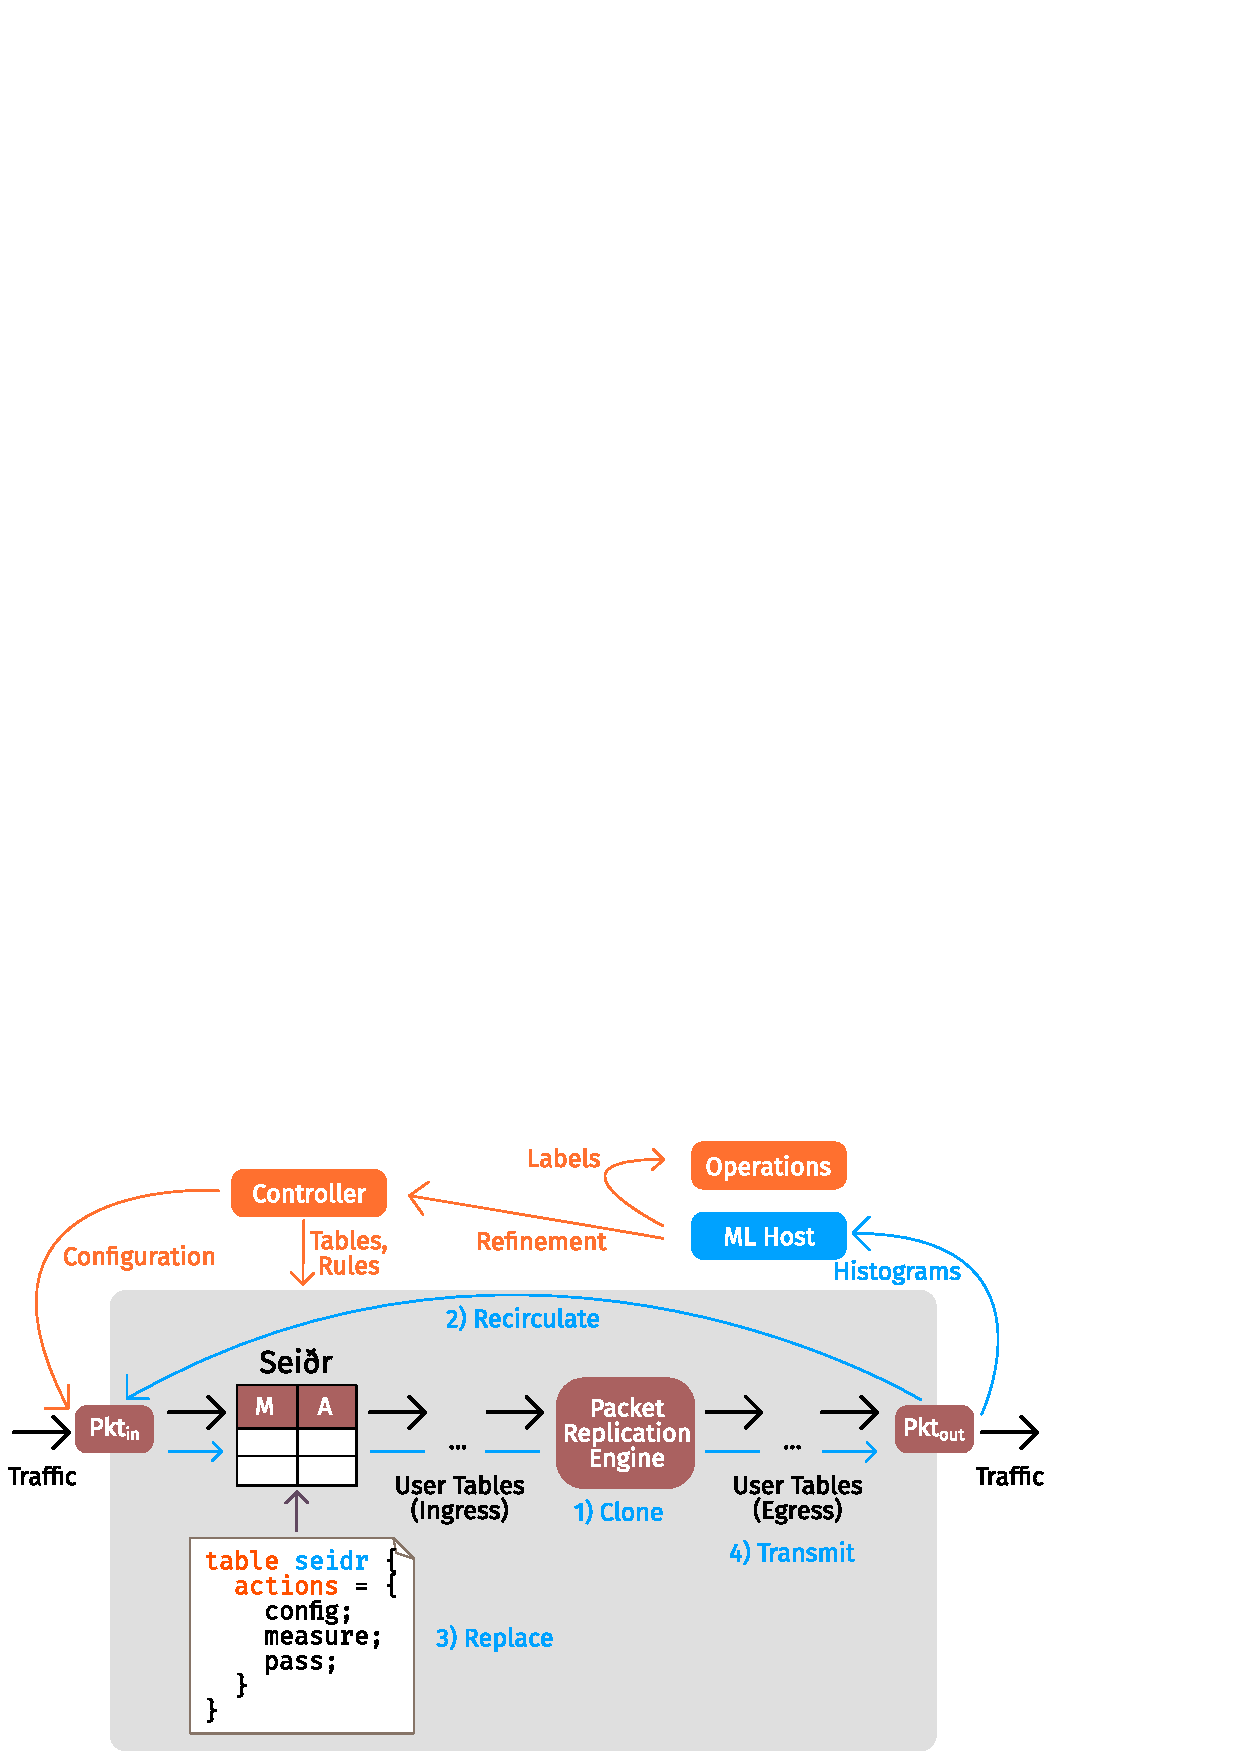
\includegraphics{diagrams/seidr/dp-arch-diagram.pdf}}
    \caption{\seidr{}'s integration with a PSA-compatible~\cite{p4-psa} dataplane.}
    \label{fig:arch}
\end{figure}

% Let's show them a histogram datastructure would look like purely with registers and how would a P4 action populate it - pseudocode or P4 snippet would be nice.

Although packet timing information is useful in understanding network and flow behaviour, without volume or packet rate reduction it is prohibitively expensive for hosts to handle each packet.
Histogramming acts as the \emph{aggregation step} which makes this class of analysis feasible in high-speed networks.
\Cref{fig:arch} demonstrates how \seidr{}, installed as an additional table in any P4 program, records and transmits inter-arrival time histograms.
The format for these histogram packets is outlined in \cref{fig:seidr-headers}; we choose to store individual buckets as \mintinline{rust}{u16}s, and the number of buckets in any histogram is fixed at compile time.
We set this to \num{100} buckets per histogram.
Packets traverse a table which requires \num{3} actions to be implemented:
\begin{enumerate}
    \item \mintinline{rust}{config} reads any matched packets as a \mintinline{rust}{seidr_cfg_t} of type \mintinline{rust}{SET_}\{ \mintinline{rust}{MIN}, \mintinline{rust}{MAX}, \mintinline{rust}{DST}, \mintinline{rust}{SRC}, \mintinline{rust}{LEN} \} by using the P4 parser.
    These update registers \numrange{1}{5} in \cref{tab:registers}, dropping any matched packets.
    
    \item \mintinline{rust}{measure} calculates the inter-arrival time, update per-flow histograms, and transmits finished histograms to the correct host. We describe its operation in \cref{alg:measure}.
    
    \item \mintinline{rust}{pass} ignores packets, and is the default action.
\end{enumerate}
Constructing \seidr{} in this manner allows the control plane to install rules to enable/disable runtime reconfiguration as needed, and to monitor as many or as few flows as desired (\ie, using wildcard rules, or exact matching).

The PSA does not have any mechanisms for generating new packets.
To circumvent this, any packet which would complete a histogram is tagged for cloning at the end of the ingress pipeline, and recirculation at egress (\cref{algline:recirc}).
This truncated copy returns to \seidr{}'s table, where we enable the relevant headers, change L2/3 fields, and write out the histogram contents (\crefrange{algline:rewrite-start}{algline:rewrite-end}).
The P4 deparser outputs the new protocol stack at egress, and transmits the histogram UDP packet into the network.
Event-driven architecture proposals~\cite{DBLP:conf/hotnets/IbanezABM19} may allow a more natural means of packet generation.

\begin{figure}
\centering
\begin{subfigure}{0.45\linewidth}
\centering
\adjustbox{max width = 0.6\linewidth}{
\begin{minipage}{\linewidth}
\begin{minted}[escapeinside=||]{rust}
|\textbf{\textcolor{Keyword}{header}}| seidr_cfg_t {
    bit<8> function;
    bit<144> payload;
}
\end{minted}
\end{minipage}
}
\end{subfigure}
\begin{subfigure}{0.45\linewidth}
\centering
\adjustbox{max width = 0.6\linewidth}{
\begin{minipage}{\linewidth}
\begin{minted}[escapeinside=||]{rust}
|\textbf{\textcolor{Keyword}{header}}| seidr_t {
    bit<128> src_ip;
    bit<128> dst_ip;
    bit<16> src_port;
    bit<16> dst_port;
    bit<16> eth_type;
    bit<BUCKETS * 16> histo;
}
\end{minted}
\end{minipage}
}
\end{subfigure}
\caption{P4 headers for \seidr{} configuration and histograms.}\label{fig:seidr-headers}
\end{figure}

\begin{algorithm}
% \vspace{-0.25cm}
% \DontPrintSemicolon
\KwData{5-tuple, P4 metadata, P4 headers, Registers}
h $\leftarrow$ hash(5-tuple)\;
index $\leftarrow$ BUCKETS * h\;
owner $\leftarrow$ HistoOwner[h]\;
\uIf{metadata.packet\_path = RECIRCULATE}{
    headers.tcp.valid $\leftarrow$ false\label{algline:rewrite-start}\;
    headers.udp.valid $\leftarrow$ true\;
    headers.seidr.valid $\leftarrow$ true\;
    copy 5-tuple into headers.seidr\;
    rewrite headers.ip, headers.udp using HistoSrc/Dest\;
    headers.seidr.histo $\leftarrow$ HistoData[index..]\;
    truncate payload\;
    zero out registers: BucketCount, HistoOwner[h], HistoData[index..]\;\label{algline:rewrite-end}
}
\ElseIf{owner = 0 \textbf{or} owner = 5-tuple}{\label{algline:owner-check}
    HistoOwner[h] $\leftarrow$ 5-tuple\;
    iat $\leftarrow$ LastTimestamp - metadata.mac\_ingress\_time\;
    \If{iat $\ge$ Min \textbf{and} iat $\le$ Max}{
        bucket $\leftarrow$ BUCKETS * (iat - Min) / (Max - Min)\;
        HistoData[index + bucket] $\leftarrow$ HistoData[index + bucket] + 1\;
        BucketCount[h] $\leftarrow$ BucketCount[h] + 1\;
        \If{BucketCount[h] = Len}{
            mark packet for cloning and recirculation\label{algline:recirc}\;
        }
    }
}

\caption{Histogram update and transmission.}\label{alg:measure}
\end{algorithm}

In the event of hash collision (\cref{algline:owner-check}), we ignore packets outside of the tracked flow to ensure that data is accurate.
As later processing and classification directly affect what decisions are made by operators or automatically taken by a policy (possibly leading to incorrect flow limits, QoS, \emph{etc.}), avoiding corruption/cross-contamination of operational data is paramount.
To gain collision resistance, Robin Hood hashing could be used up to a maximum distance in the table, treating a zeroed owner as empty and an illegal source IP as a tombstone value.

\begin{table}
    \centering
    \caption{Register map (Datatype, Amount) for an $h$-bit hash.}
    \resizebox{\linewidth}{!}{\begin{tabular}{@{}ccccccccc@{}}\toprule
        Min & Max & Length & HistoSrc & HistoDest & BucketCount & LastTimestamp & HistoOwner & HistoData \\ \midrule
        \mintinline{rust}{u16} & \mintinline{rust}{u16} & \mintinline{rust}{u16} & \mintinline{rust}{u16 + u128} & \mintinline{rust}{u16 + u128} & \mintinline{rust}{u16} & \mintinline{rust}{u64} & \mintinline{rust}{3 * u16 + 2 * u128} & \mintinline{rust}{BUCKETS * u16} \\
        1 & 1 & 1 & 1 & 1 & $2^h$ & $2^h$ & $2^h$ & $2^h$ \\ \bottomrule
    \end{tabular}}
    \label{tab:registers}
\end{table}

% Basic Logic:
% \begin{itemize}
%     \item table 1: three actions
%     \begin{itemize}
%         \item config: set R1 or R2 (controller installs rule matching a specific port/ip combo)
%         \item measure: take ingress timestamp from metadata, do stuff, write into lasttime, add to bucket and total if within bounds
%         \item pass (default)
%     \end{itemize}
%     \item then pass onto rest of tables
%     \item Why do it this way? can make it all or nothing through control plane.
%     \item How to write and send packet? Same trick as ESNET? (recirc w/ custom metadata to transform pkt)
% \end{itemize}

% ?? NOTE: See PSA \cite{p4-psa} for register format. Some papers, like Dapper, suggest that hash tables should be possible? That would work out very well in our benefit.

% ?? What is configurable? Min, max of the histogramming range

This design allows runtime configuration of all aspects save for the bucket count; at runtime, the only way to increase bucket resolution is to examine a smaller region of IATs.
While in theory this could be configured below a maximum compiled into the firmware, the difficulties introduced in classification/data processing make this infeasible.
Unless using stream-capable classifiers such as LSTMs~\cite{DBLP:journals/neco/HochreiterS97}, changing the input size requires retraining from scratch since new neuron weights must be added and structural properties of the input data change.
Increasing the bucket count requires new firmware installation, as many dataplane P4 implementations cannot allocate variable-length stores due to the lack of a dynamic allocator.

\begin{figure}[t]
    \centering
    \begin{subfigure}[t]{0.49\linewidth}
        \centering
        \resizebox{\linewidth}{!}{\includegraphics{plots/seidr/dt-cubic-1000-app.pdf}}
        \subcaption{TCP Cubic}
        \label{fig:cubic-hist-app}
    \end{subfigure}
    \begin{subfigure}[t]{0.49\linewidth}
        \centering
        \resizebox{\linewidth}{!}{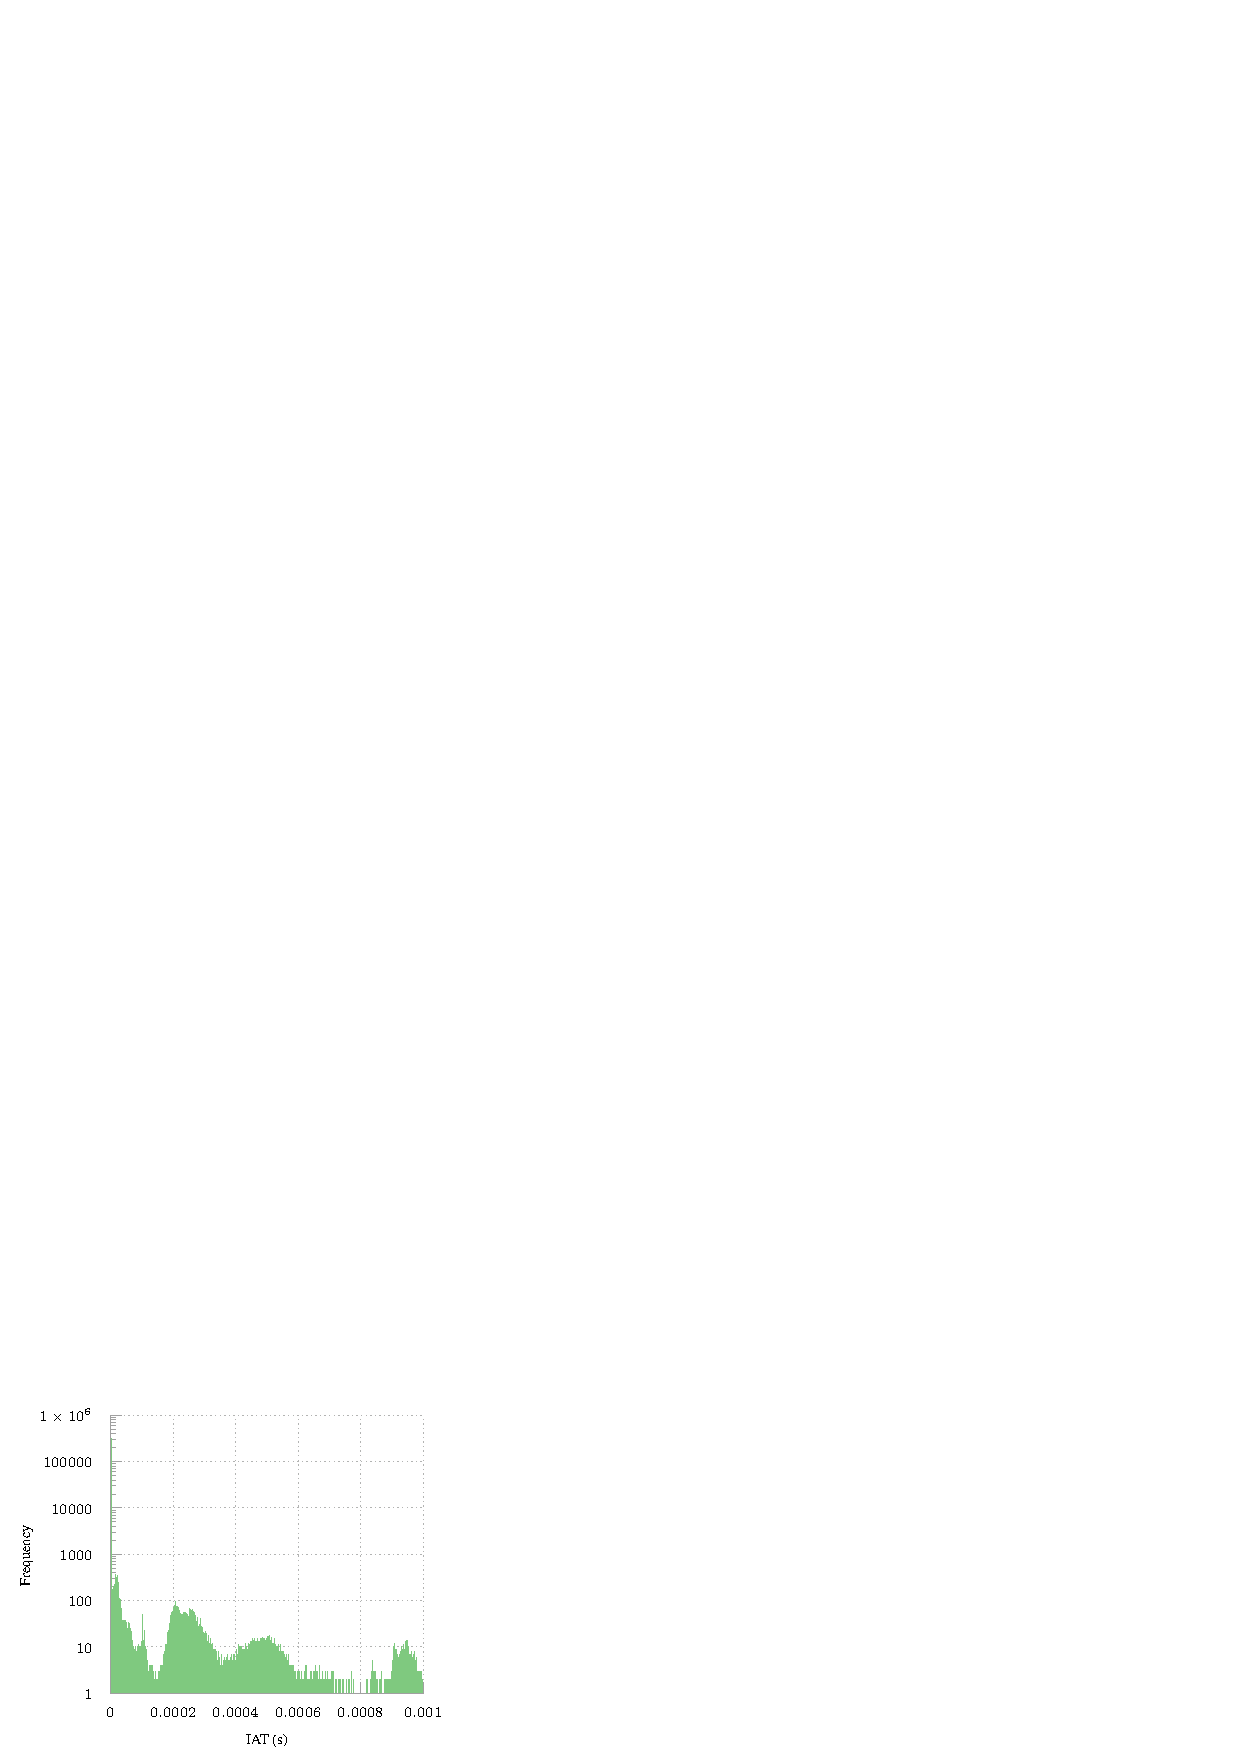
\includegraphics{plots/seidr/dt-bbr-1000-app.pdf}}
        \subcaption{TCP BBR}
        \label{fig:bbr-hist-app}
    \end{subfigure}
    \caption{Example dataplane histograms showing visible differences in inter-arrival times of selected TCP flavours. Our ML solutions are trained to programmatically identify such differences.}
    \label{fig:tcp-hist-app}
\end{figure}

As an example of dataplane-generated histograms, \cref{fig:tcp-hist-app} shows the distribution of inter-arrival times between two TCP congestion control algorithms. The visible differences are programmatically identified using our ML algorithms.

\subsection{Accurate, Precise and High-Resolution Timestamping}

Precise timestamps are critical when detecting temporal properties of flow behaviour, such as microbursts or inferring flow congestion control algorithms.
It is especially important in high speed (\SI{100}{\giga\bit\per\second}) networks, where there can be as little as \SI{6.7}{\nano\second} between packets that need to be analysed.
With a Linux-based software solution (\eg, reading packets from a link with \emph{tcpdump}), the Linux kernel can only provide microsecond-level accuracy with precision in the order of \SI{100}{\micro\second}~\cite{kundel2020p4sta}.
DPDK improves on this, increasing the accuracy to \SI{100}{\nano\second} in the best case~\cite{primorac2017measure}.
However, today's dataplane devices (\eg, Netronome SmartNICs, NetFPGA SUME) allow nanosecond-accurate timestamps to be retrieved from the \emph{Media Access Control} (MAC) modules with a precision of \SI{10}{\nano\second}~\cite{kundel2020p4sta}, a timestamp property \seidr{} relies upon.

% Some platforms provide picosecond-level precision and many solutions allow time synchronisation between multiple devices using the IEEE 1588-2002 (Precision Time Protocol) standard.



\section{TCP congestion control classification}\label{sec:seidr-tcpcc}


% We present an example of first-stage analysis performed for each flow and each packet---stateful TCP analysis.
% This includes numerous metrics which are considered standard when measured at connection endpoints, yet are difficult or invite numerous issues when performed in the network (of which we include a discussion on drawbacks and, curiously, benefits).
% The introduction of accurate timestamps allows us to explore rate-monitoring at a per-packet level, a new view of flow behaviour which may enable flow and hardware characterisation.

% \subsection{Per-Packet Rate Monitoring}

% \begin{figure*}
%     \centering
%     \begin{subfigure}[t]{0.49\linewidth}
%         \centering
%         \resizebox{0.5\linewidth}{!}{
% 	    \begin{tikzpicture}
%     		[packet/.style={draw, fill=uofgsunshine}]
% 		    \node[packet] (p1) {$p_1$: 1500B};
% 		    \node[packet, right= 1cm of p1] (p2) {$p_2$: 800B};
		
% 		    \node at ($(p1.south west) - (0,1)$) (t1) {$t_1$};
% 		    \node at ($(p2.south west) - (0,1)$) (t2) {$t_2$};
		
% 		    \draw[-, dotted] (t1.north)--(p1.south west);
% 		    \draw[-, dotted] (t2.north)--(p2.south west);
		
%     		\draw[<->] (t1.north) -- node[below]{$\mathit{dt}$} (t2.north);
% 	    	\draw[<->] ($(t1.north) + (0,0.2)$) -- node[above]{$s$} ($(t1.north) + (1.8,0.2)$);
% 		    \draw[<->] ($(t1.north) + (1.8,0.2)$) -- node[above]{$g$} ($(t2.north) + (0,0.2)$);
% 	    \end{tikzpicture} 
% 	}
%     \caption{\centering Per-packet rate, visualised. Note that $p_1$ and $p_2$ are not necessarily packets from the same flow.}
%     \label{fig:per-packet-rate}
%     \end{subfigure}
%     \begin{subfigure}[t]{0.49\linewidth}
%     \centering
%     \resizebox{0.9\linewidth}{!}{
% 		\begin{tikzpicture}
% 		[packet/.style={draw, fill=uofgsunshine}]
% 		\node[packet] (p1) {$p_1$: 1500B};
% 		\node[packet, right= 1cm of p1] (p2) {$p_2$: 800B};
% 		\node[right= 1cm of p2] (p3) {...};
% 		\node[packet, right= 1cm of p3] (p4) {$p_{n-1}$: 1500B};
% 		\node[packet, right= 1cm of p4] (p5) {$p_n$: 1500B};
		
% 		\node at ($(p1.south west) - (0,1)$) (t1) {$t_1$};
% 		\node at ($(p2.south west) - (0,1)$) (t2) {$t_2$};
% 		\node at ($(p4.south west) - (0,1)$) (t4) {$t_{n-1}$};
% 		\node at ($(p5.south west) - (0,1)$) (t5) {$t_{n}$};
		
% 		\draw[-, dotted] (t1.north)--(p1.south west);
% 		\draw[-, dotted] (t2.north)--(p2.south west);
% 		\draw[-, dotted] (t4.north)--(p4.south west);
% 		\draw[-, dotted] (t5.north)--(p5.south west);

%         \draw[<->] ($(t2.south) + (0,-0.25)$) -- node[above]{$s$} ($(t2.south) + (6.25,-0.25)$);
%         \draw[<->] ($(t2.south) + (6.25,-0.25)$) -- node[above]{$g$} ($(t5.south) + (0,-0.25)$);
% 		\draw[-, thick] ($(t2.south) - (0,0.5)$) -- node[below]{$W$} ($(t5.south) - (0,0.5)$);
% 		\end{tikzpicture} 
% 	}
%     \caption{\centering Sliding window rate, visualised. Rate estimates are computed using the sizes of the last $W$ packets seen in the current flow. Packets $p_2$ and $p_{n-1}$ belong to the same flow, but $p_n$ is not assumed to.}
%     \label{fig:sliding-window-rate}
%     \end{subfigure}
%     \caption{Comparison of per-packet and sliding window rates. The lengths of packets and inter-packet gaps are not to scale, and are purely demonstrative.}
%     \label{fig:pr-vs-slide}
% \end{figure*}

% Associating each packet with a high-resolution timestamp allows us to introduce the notion of a \emph{per-packet rate}.
% Assuming a packet with size $p$ arrives at time $t_1$ and is followed by another packet (potentially from another flow) which arrives at $t_2$, we measure $\mathit{dt}=t_2-t_1$ for this packet.
% Supposing this first packet spends time $s$ on the wire and assuming that the inter-packet gap $g$ is negligible compared to the length of a packet, then $\mathit{s} = \mathit{dt} - g \approx \mathit{dt}$.
% This packet then has a point rate, $r$:
% \begin{equation}
%     r = \frac{p}{s} \approx \frac{p}{\mathit{dt}}
% \end{equation}
% \Cref{fig:pr-vs-slide} demonstrates how this timing information arises, contrasted with sliding-window rate measurements taken over a longer time period.
% This assumes almost back-to-back traffic, which is realistic in our deployment environment, but to the best of our knowledge no programmable switches expose the timestamp at which the final bit of a packet has been ingested.
% Such a timestamp would allow exact measurement of $s$.

% % ?? we need to be clear about the unintuitive nature of these measurements, include a quick sketch proof which shows that the weighted average of a set of point rates is analytically identical to the sliding window rate/throughput taken over the same period of time.
% While this is an interesting measure to associate with each packet, considering how best to view such rates in aggregate can be counter-intuitive.
% Viewing these rates as time series data reveals interesting distributional characteristics which disagree starkly with our understanding of a flow's rate---for instance, clusters which suggest a different mean.
% Suppose we have a set of measurement indices $C$ with no gaps captured between $t$ and $t'$, partitioned into flows $C = F_1 \cup \dots \cup F_p$.
% To correctly combine a set of point measurements for a flow $F_i$ into an average rate $\overline{r}_{F_i}$, we compute:
% \begin{equation}
%     \overline{r}_{F_i} = \frac{\sum_{a \in F_i} \mathit{dt}_a r_a}{\sum_{c \in C} \mathit{dt}_c}.
% \end{equation}
% In the instance that only one flow is captured (\emph{i.e.}, $F_i = C$), this is a weighted average over point rates, using the $\mathit{dt}$ measured between each packet and the next packet in the same flow as its weight.
% Similarly, this is analytically equivalent to the sliding-window rate measured over the same set of packets:
% \begin{equation}
%     \frac{\sum_{a \in F_i} \mathit{dt}_a r_a}{\sum_{a \in F_i} \mathit{dt}_a} \simeq \frac{\sum_{a \in F_i} p_a}{t' - t}.
% \end{equation}
% % \begin{proof}
% % Given a set of contiguous measurements from the same flow $S \subseteq \mathbb{Z}$, admitting $p_s$, $r_s$, $\mathit{IAT}_s$ and $t_s$, the weighted average of point rates is then
% % $$
% % \overline{r}_S = \frac{\sum_{s \in S} \mathit{IAT}_s r_s}{\sum_{s \in S} \mathit{IAT}_s}
% % $$
% % The sliding-window average:
% % $$
% % \overline{r}_S = \frac{\sum_{s \in S} \mathit{IAT}_s r_s}{\sum_{s \in S} \mathit{IAT}_s}
% % $$
% % \end{proof}

% We assume that inter-packet gaps will be negligible (\emph{i.e.}, that the link is never in a state of very low utilisation), due to typically high utilisation on a WAN.
% % Similarly, we need to discuss the effects of selective monitoring or an abundance of UDP/ICMP traffic (which will distort $dt$s).
% However, this assumption can be distorted if selective TCP flow monitoring is used, or if UDP/ICMP traffic is overabundant; both these scenarios create larger gaps between TCP packets of interest, inflating $g$ to the point where it is comparable in size to $s$.
% This has an impact on our notion of per-packet rates, but not inter-arrival times or other such dependent metrics.
% The effect is small on sliding window rates, particularly at larger window sizes.
% ?? Justify. On paper, it looked like error term was O(1/n), O(g) for an n packet window.


% \section{Inter-Arrival Time}

% Having assigned each packet in a flow with a nanosecond-accurate timestamp ?? tbc

\Cref{fig:tcp-hist-app} suggests that a notable use-case for this type of measurement is \emph{congestion control algorithm} (CCA) detection.
In a TCP connection, each machine is free to choose the CCA it uses to send bytes, and thus how it responds to network congestion signals.
This choice is local, and so is invisible to the other machine (and the network).
In datacentre networks, operators choose these to ensure optimal behaviour.
In a transit network or large WAN however, these hosts (and thus the CCAs in use) are outside the control of network operators, which introduces difficulties when CCA interactions lead to \emph{unfairness}.
Consider the recent (and widespread) introduction of \emph{TCP BBR}~\parencite{DBLP:journals/queue/CardwellCGYJ16}.
\emph{BBR} is a delay/model-based CCA which converges on a fair share of bottleneck bandwidth by reducing its rate if the round-trip time increases, while periodically attempting to increase send rate to account for path/load changes.
However, \emph{BBR} traffic can consume \SI{40}{\percent} of link capacity when multiplexed with loss-based CCAs, regardless of the number of competing flows~\parencite{DBLP:conf/imc/WareMSS19}. 
When ensuring fair transit to all flows, this is hardly a desirable outcome; in fact, it's one which may frustrate clients or violate SLAs.

A curious property of \emph{BBR}'s algorithm which sets it apart from other variants is that packet transmission is \emph{timer-based}.
\texttt{send(packet)}, as defined in the canonical algorithm, asks that on transmission of a packet, the sender should wait for the estimated time that packet would take to reach the recipient.
For instance, at an estimated bottleneck bandwidth of \SI{8}{\mega\bit\per\second}, a \SI{1024}{\kilo\byte} packet would hold back the next packet in the flow until \SI{976.6}{\micro\second} had elapsed.
When packet sizes remain similar this causes strongly periodic behaviour, while mode switches in the \emph{BBR} algorithm cause these periodic bands to shift up or down accordingly.
This effect is stronger than in existing loss- and delay-based algorithms which remain intrinsically tied to the notion of a congestion window (where release of buffered packets follows the receipt of ACK messages).
As a result, timing behaviour of past CCAs may be influenced by (the lack of) packet pacing, periodic components might be made noisier by jitter along the return path, or the behaviour of the receiver might add further noise.

This high-level analysis of \emph{BBR} gives us a strong feature to use as the basis for classification: the \emph{inter-arrival times} (IATs) for each packet in a flow.
We have two options for processing this for classification: we may use a compressed, fixed-size representation such as histograms to capture the aggregate distribution, or we may attempt to capture structural behaviour by using a variable-length stream of IATs.
In many networks, the data and packet rate reduction offered by the former is required to make this possible.
Indeed, in-switch aggregation has seen great success in aiding ML for training~\parencite{DBLP:conf/isca/LiLYCSH19}, and direct execution~\parencite{DBLP:conf/hotnets/XiongZ19}.
We make use of the following standard classification algorithms on a fixed-size representation to attempt to single out the CCA in use:

\begin{itemize}
    \item \emph{$k$-Nearest Neighbours ($k$-NN)}. A simple and well-understood classifier which assigns labels based on the closest members of the training corpus (\ie, by the $L_2$ metric). Linear memory cost in amount of training data, and no training cost other than loading all data points, but capable of learning complex decision boundaries on fixed-length input.
    
    \item \emph{Convolutional Neural Networks (CNNs)}. A neural network approach which learns convolution kernels to classify fixed-length data, particularly when recognising spatial features. Memory cost is fixed for a given architecture irrespective of training data, with a high training cost.
\end{itemize}
% \fakepara{Long Short-Term Memory~\parencite{DBLP:journals/neco/HochreiterS97} units (LSTMs)} A class of recurrent neural network used for stream classification, forecasting, and prediction of variable-length data. Memory cost is fixed, with longer training times (and more data required) than similarly sized CNNs.
% Of these, we apply $k$-NN and CNNs to histograms of packet IATs, and LSTMS to raw IAT streams.

When examining $k$-NN classifiers, we measured accuracy across choices of $k \in \left[2, 8\right]$.
We found $k=2$ to be the most effective choice with our input data using the $L_2$ metric.
Our CNN architecture is described in \cref{tab:cnn-arch}, using ReLu activation and $1 \times 1$ stride in convolutional layers unless stated otherwise.
Training occurred over 5 epochs using the Adam optimiser with categorical cross-entropy as a loss metric, and a batch size of \num{64} histograms (\num{8} for full sequences due to the smaller data volume).
For \emph{BBR vs.\ Cubic}, the complete model consists of \num{104898} 32-bit floating-point parameters (\SI{409.76}{\kibi\byte}), while the full classification task adds a further \num{130} parameters (\SI{0.51}{\kibi\byte}).

\begin{table}
    \centering
    \caption{CNN architecture for \num{100}-entry histograms.}
    \resizebox{0.7\linewidth}{!}{\begin{tabular}{@{}cccc@{}}\toprule
        Layer & Nodes/Filters & Filter Size & Output Dimension \\ \midrule
        Conv2D & 32 & $(3 \times 1)$ & $(98 \times 1 \times 32)$ \\
        MaxPool & --- & $(2 \times 1)$ & $(49 \times 1 \times 32)$ \\
        Conv2D & 64 & $(3 \times 1)$ & $(47 \times 1 \times 64)$ \\
        MaxPool & --- & $(2 \times 1)$ & $(23 \times 1 \times 64)$ \\
        Conv2D & 64 & $(3 \times 1)$ & $(21 \times 1 \times 64)$ \\
        Flatten & --- & --- & \num{1344} \\
        Dense & 64 & --- & \num{64} \\
        Dense (Softmax) & $n_\mathit{classes}$ & --- & $n_\mathit{classes}$ \\
        \bottomrule
    \end{tabular}}
    \label{tab:cnn-arch}
\end{table}


\section{Evaluation}\label{sec:seidr-evaluation}
%Traffic is played back from hosts via Tcpreplay at a bandwidth assigned uniformly from a `good' or `bad' distribution, each using the same pcap file with source and destination IP addresses rewritten.

This work is most naturally compared against Marl, introduced by \textcite{DBLP:journals/eaai/MalialisK15}, the state-of-the-art in \gls{acr:rl}-based \gls{acr:ddos} prevention.
We are most interested in seeing how their approach contrasts with the new agent designs across different topologies and workloads.
Different network environments will also impose different levels of host density, where popular web servers may have orders of magnitude more clients than egress points from their network---I aim to show how these characteristics affect performance and learning rate.
Marl is known to outperform the AIMD~\parencite{DBLP:journals/ton/YauLLY05} strategy, yet the state of the art has long since moved on.
To paint a more current picture, I compare this work against an effective modern approach, \emph{SPIFFY}~\parencite{DBLP:conf/ndss/KangGS16}.
SPIFFY tests a proportion of flows by routing them through an alternate path with higher bandwidth, observing how their speed changes some time later.
This comparison lets us position our new agent designs against the state of the art, observing that SPIFFY has a similar mode of interaction to \gls{acr:rl}-based systems (taking action, observing an effect, and acting once again) and does not rely on protocol characteristics or signatures.
In reimplementing SPIFFY, I make the simplifying assumption that a suitable unused path exists (with identical bandwidth to the server's link).
\qty{10}{\percent} of active flows were tested at a time (according to the authors' observation that there is a factor of \qty{10}{\times} difference between the ideal and achieved bandwidth expansion), excluding flows below \qty{50}{\kilo\bit\per\second} and requiring a \qty{3}{\times} expansion from legitimate flows, making a judgement after \qty{5}{\second}.

To test this, I made use of both traffic models introduced in \cref{sec:a-new-normal} (Opus and \gls{acr:tcp}), both topologies discussed below (1-dest vs.\ Fat-Tree), and vary the amount of hosts typically communicating over each agent's ingress/egress node.
Additionally, these new models were evaluated in multi-agent mode (\emph{separate}, no model sharing), and in single-agent mode (\emph{single}, zero-cost perfect information sharing).
In each case, the algorithm's performance was averaged over \num{10} episodes of length \num{10000} timesteps (setting each agent's $\wvec{}=\mathbf{0}$ between episodes).
Host allocations at the beginning of each episode were generated pseudorandomly to ensure fairness between episodes---a host is malicious with probability $\operatorname{P}\left(\mathit{malicious}\right)$, and is benign otherwise.
Benign hosts generate traffic according to either \cref{sec:tcp-http-traffic-model,sec:udp-opus-traffic-model} depending on the experiment, while malicious hosts generate traffic as described in \cref{sec:attack-traffic-model} (both at experiment-dependent rates).

All experiments were executed on Ubuntu 18.04.2 LTS (GNU/Linux 4.4.3-040403-generic x86\_64), using an Intel Core i7-6700K (\qtyproduct[product-units=single]{4 x 4.2}{\giga\hertz}) which had \SI{32}{\gibi\byte} of \gls{acr:ram}.
%All code underpinning these findings is available on a public repository\footnote{\url{https://github.com/FelixMcFelix/rln-dc-ddos-paper}}.
%All code underpinning these findings is available on a public repository.\footnote{Private until publication.}

\subsection{Single destination}\label{sec:single-dest}
%?? Move description of tree topol to here.
The network is tree-structured, where one server $s$ connects through a dedicated switch to $k$ team leader switches, each connected to $\ell$ intermediate switches, which in turn each connect to $m$ egress switches.
We then have $N_{\mathit{hosts}} = k \ell m n$.
\Cref{fig:marl-topol} demonstrates this.
%Although \citeauthor{DBLP:journals/ccr/MahajanBFIPS02a}, the originators of this topology, make it clear that it exists as a fairly unrepresentative example \cite{DBLP:journals/ccr/MahajanBFIPS02a}, it remains the case that such a network topology allows for functional testing, and indeed is illustrative of one way in which attack traffic might aggregate in the network.
%It is hard, however, to argue its relevance to specific classes of victim or to reason about the interactions it might have with dependent applications.
%We aim to address this through \cref{sec:performance-in-an-emulated-environment}.
The network topology was configured using $k=2$ teams, $\ell=3$ intermediate nodes per team, $m=2$ agents per intermediate node, and $n \in \{2, 4, 8, 16\}$ hosts per learner.
This is a slight simplification of \Textcite{DBLP:journals/eaai/MalialisK15}'s \textquote{online} experiment, choosing fewer teams but remaining as a single server with a fan-out network.
%The algorithm parameters were set at $\gamma=0$ (leading to opportunistic behaviour), $\alpha=0.05$, having linearly annealed $\epsilon=0.2 \rightarrow 0$ by $t=3000$.
%Benign and malicious hosts uploaded between \SIrange{0}{1}{\mega\bit\per\second} and \SIrange{2.5}{6}{\mega\bit\per\second} respectively, and hosts were redrawn at each episode's start with $\operatorname{P}(\mathit{malicious})=0.4$.
%$U_s$  $k \ell mn+2$ \si{\mega\bit\per\second}.
%The performance of each choice of $n$ was averaged over \num{10} episodes of length \num{10000} timesteps (setting each agent's $\wvec{}=\bm{0}$ between episodes).
%Host allocations were generated pseudorandomly to ensure fairness between choices of $n$.
%These parameter choices match those of the original study to enable direct comparison, and are (to the best of our knowledge) arbitrary, but we justify our range of $n$ as capturing increasing scales of host activity.

\begin{figure}
	\centering
	\resizebox{0.9\linewidth}{!}{\begin{tikzpicture}[
	texts/.style = {text=black},
	labeltexts/.style = {text=uofgsandstone},
	treeline/.style = {draw=uofgburgundy},
	treenode/.style = {texts, circle, centered, fill=white, treeline},
	load/.style = {fill=uofgcobalt},
	loadhide/.style = {fill=uofgcobalt!40!white},
	external/.style = {fill=uofgrust},
	externalhide/.style = {fill=uofgrust!40!white},
	hideline/.style = {draw=uofgsandstone!40!white},
	hidenode/.style = {treenode, hideline},
	grow'=right
]
	\node[treenode, label={[texts]above:Server}] (root) {}
	child [treeline] { node [treenode, label={[texts]above:Core}] (sswitch) {}
		child [treeline] { node [treenode, label={[texts]above:Leader}] (teaml) {} 
			child [treeline] { node [treenode, label={[texts]above:Intermediate}] (inter) {}
				child [treeline] { node [treenode, load, label={[texts]above:Agent/Egress}] (agent) {}
					child [treeline] { node [treenode, external] (extern) {}
						child [treeline] { node [treenode, external, label={[texts]above:Host}] (host) {} }
						child [hideline] { node [hidenode, externalhide] (endhost) {} }
					}
				}
				child [hideline] { node [hidenode, loadhide] (endagent) {} }
			}
			child [hideline] { node [hidenode] (endinter) {} }
		}
		child [hideline] { node [hidenode] (endteaml) {} }
		edge from parent
		node[below, labeltexts] {$U_s$}
	};
	
	%\draw[-] (teaml) -- (endteaml);
	\node [labeltexts] (kdots) at ($(teaml)!0.5!(endteaml)$) {$\rvdots$};
	\node [labeltexts, right = -0.1cm of kdots] {$k$};
	\node [labeltexts] (ldots) at ($(inter)!0.5!(endinter)$) {$\rvdots$};
	\node [labeltexts, right = -0.1cm of ldots] {$\ell$};
	\node [labeltexts] (mdots) at ($(agent)!0.5!(endagent)$) {$\rvdots$};
	\node [labeltexts, right = -0.1cm of mdots] {$m$};
	\node [labeltexts] (ndots) at ($(host)!0.5!(endhost)$) {$\rvdots$};
	\node [labeltexts, right = -0.1cm of ndots] {$n$};
\end{tikzpicture}}
	\caption[Tree-structured network topology diagram for evaluating a single-destination network.]{
		Network topology diagram, showing how the server and its core switch's $k$ teams are structured, with $\ell$ intermediate routers per team, connected to $m$ agents which each moderate $n$ hosts beyond a single external switch.
		%	Empty nodes are considered to be internal.
		Red nodes are external, and each blue node hosts an agent.
		\label{fig:marl-topol}
	}
\end{figure}

\subsection{Multiple destinations}
The previous topology allows for direct comparison against the state-of-the-art, and indeed is illustrative of one way in which attack traffic might aggregate in the network.
It is hard, however, to argue its relevance to specific classes of victim or to reason about the interactions it might have with dependent applications.
In contrast, the fat-tree topology~\parencite{DBLP:conf/sigcomm/Al-FaresLV08} sees regular use in real-world data centres and scales well horizontally.
%?? Come up with description of fat-tree (multi-dest) topol.
%?? Why fat tree? regularly appears in modern datacentres.
%?? $k=4$ fat-tree , with one pod hosting two servers $s_0,s_1$.
We use a $k=4$ fat-tree, with one pod hosting two servers $s_0$ and $s_1$.
$n$ external hosts connect through each core switch (where agents are hosted), and communicate with $s_0, s_1$ uniformly randomly.
Both servers host identical services.
We set $n \in \{6, 12, 24, 48\}$ hosts per learner (keeping $N_{\mathit{hosts}}$ identical to each tier of the single-host topology), and restrict $U_{s_0} = U_{s_1} = U_s / 2$.

\subsection{Parameters}
The algorithm parameters were set at $\alpha=0.05$, linearly annealing $\epsilon=$ \num{0.2} $\rightarrow$ 0 by $t=$~\num{3000} in the case of Marl (\num{8000} actions per agent in the \emph{Instant/Guarded} models).

Benign hosts each occupied \qtyrange{0}{1}{\mega\bit\per\second}, and hosts were redrawn at each episode's start with $\operatorname{P}(\mathit{malicious})=$~\num{0.4}.
%The original introduction of this approach to direct-control reinforcement learning as introduced by \textcite{DBLP:journals/eaai/MalialisK15} fails to consider key cases: the absence of a suitable heuristic classifier $g(\cdot)$, disjoint ranges of traffic distribution (i.e., the presence of benign heavy-hitters), the accurate simulation of TCP-like behaviour (and its effects on collateral damage), and high densities of hosts at egress points.
%?? Why? ...
%Of these, the latter two are most deserving of a closer investigation, as they have stronger implications for wide-scale deployment.
%These are important issues, particularly when we consider real-world deployment.
%Heuristic estimates of traffic legitimacy come with computational cost and couple the reward function to the accuracy of the estimator, hosts often show diversity in their own traffic patterns (perhaps being multi-modal), and it is known that TCP is the most used transport protocol for Internet traffic \cite{DBLP:conf/saint/ZhangDJC09}.
%?? NEED TO VERIFY VOLUME OF CONGESTION-AWARE PROTOCOLS
Malicious hosts each sent \qtyrange{2.5}{6}{\mega\bit\per\second} when attacking \gls{acr:udp} traffic, though this was increased to \qtyrange{4}{7}{\mega\bit\per\second} when using \gls{acr:tcp}-like traffic (to meaningfully impact benign flows).
Given $n$ and $\operatorname{P}(\mathit{malicious})$, we see an expected malicious bandwidth \numrange{1.27}{1.87} and \qtyrange{2.03}{2.18}{\times} $U_s$ respectively.
%The expected fraction of $U_s$ consumed by each host is \SI{21.5}{\percent} for $n=2$, and \SI{2.84}{\percent} for $n=16$.
For these choices of $n$ in both topologies, we observe $N_{\mathit{hosts}} \in \left\{24, 48, 96, 192\right\}$, and an expected number of malicious hosts $\mathbb{E}\left[N_{\mathit{attackers}}\right] \in \left\{9.6, 19.2, 38.4, 76.8\right\}$.
For the largest choice of $n$, we see an expected total attack traffic $\mathbb{E}\left[V_{\mathit{attack}}\right] =$ \qtylist{334.05;422.4}{\mega\bit\per\second} for Opus and \gls{acr:http} traffic respectively.

$U_s$ was fixed at $N_{\mathit{hosts}}+2$ \unit{\mega\bit\per\second} (to account for burstiness), and each link had a delay of \qty{10}{\milli\second}.
All links had unbounded capacity, save for each server-switch.
These parameters match those of the original study to enable direct comparison, and many are (to the best of our knowledge) arbitrary, but I justify the range of $n$ as capturing increasing scales of host activity.

% \section{Related Work}\label{sec:related}
% %?? Try and compare my work here when possible?

\fakepara{DDoS Prevention}
\Textcite{DBLP:conf/lcn/BragaMP10} examine the detection of flooding DDoS attacks through \emph{self-organising maps}, using SDN to gather statistics effectively.
Many of their features aren't overly relevant, as their focus is not active defence or discovering \emph{which} hosts contribute to an attack.
%?? Actually talk about Marl (???) to appease reviewer \#1.
The closest available approach within this field is that of \textcite{DBLP:journals/eaai/MalialisK15} (whom we have positioned our work against), and their contribution in applying RL to the task of intrusion prevention is significant: their work helps to show the viability of live, adaptive, feedback-loop-like control of the network to detect and prevent DDoS attacks.
They create a tree overlay topology (subdivided into teams), where each agent applies packet drop to \emph{all} flows inbound to a protected server.
%?? Recap their flaws, since they've been cut form every other aspect.
Our results show that their technique underperforms at high host density and when congestion-aware traffic dominates---that their results do not demonstrate this suggests an evaluation driven purely by traces (rather than live application dynamics).

\emph{SPIFFY} \cite{DBLP:conf/ndss/KangGS16} aims to remedy transit-link attacks by observing how flows from each source respond to a sudden increase in available bandwidth.
\Citeauthor{DBLP:conf/ndss/KangGS16} realise that bots participating in an attack are often unable to match this bandwidth expansion (having already saturated the capacity of their outbound links), while legitimate flows typically speed up to match the new fair-share rate.
%Attackers must either be detected or reduce the throughput of each bot, increasing the cost of launching an attack.
%Unlike our approach (and due to the class of attacks it is designed to defend against), SPIFFY is intended to be deployed within ASes, although .
A weakness of their approach is that computing a route to measure bandwidth expansion on real networks can be costly (up to \SI{14}{\second} for the Cogent topology), and that the low expansion factors in real network can require more ``rounds'' of filtering.
By contrast, our approach takes a constant time to compute an action for a flow regardless of topology size.
Their assumptions about traffic response to such bandwidth expansion do not hold for constant bitrate flows (e.g., VoIP) and may not extend to HTTP DASH flows, both of which make up a sizeable proportion of network traffic.

\emph{Athena} \cite{DBLP:conf/dsn/LeeKSPY17} is a generalised SDN framework for intrusion detection, but has shown the use of a \emph{k-nearest neighbours} classifier to detect individual attack flows.
Although heavyweight (and proven to be effective compared with \textcite{DBLP:conf/lcn/BragaMP10}), their comparison against SPIFFY lacks the quantitative evidence required to understand how the system compares.
\Textcite{DBLP:conf/sp/SmithS18} use AS-level routing to tackle both transit-link and flooding-based attacks.
This view is taken due to the perceived cost of per-stream classification and inherent sensitivity to adversarial examples.
The approach is creative, relying upon BGP \emph{fraudulent route reverse poisoning} to preserve traffic to a target AS, but unlike SPIFFY the approach doesn't actually \emph{remove} the congestion.
Because of this, flooding-based attacks aren't fully alleviated.

%?? Abuses of RL 
\fakepara{RL in Networks}
Earnest, well-considered application of RL towards the challenge of intrusion prevention has seen comparatively little examination.
Past work treats the paradigm as a traditional classifier for anomaly detection \cite{shamshirband2014anomaly} and DDoS prevention \cite{DBLP:conf/mates/ServinK08}.
Given that the main strengths of RL techniques are the ability to control ongoing interaction and adapt by observing the concrete effects of actions, such works don't apply the rich literature on the subject to its fullest potential.

For categorising how RL fits into solving problems, we label works as direct- or indirect-control RL.
A \emph{direct-control} RL problem is one where the RL agent(s) learn optimal control over a set of actions as the \emph{primary} defence or decision-maker---requiring measurements, reward functions and action sets tailored for this purpose.
%We feel there is a shortage of work in this category at present, at least in the field of networks.
To date, the best-fitting example we have encountered is that of \textcite{DBLP:journals/eaai/MalialisK15}.
An \emph{indirect-control} RL problem is one where agents act in service to \emph{another technique} responsible for decision-making, optimising or generalising aspects of its operation beyond that of hand-coded heuristics.
A past example includes learning when best to share knowledge between \emph{hidden Markov model} anomaly detectors \cite{DBLP:conf/paisi/XuSH07}.
%The position of this work is weakened by its reliance on the problematic `DARPA99' dataset \cite{DARPA-IDD, DBLP:conf/cisda/TavallaeeBLG09, DBLP:conf/sp/SommerP10}, but the idea itself is well-treated and this acts as a driver for improvements in this direction.
This work is weakened by its reliance on the problematic `DARPA99' dataset \cite{DBLP:conf/sp/SommerP10}, but the idea itself is well-treated.
Outside of intrusion detection, there has been growing interest in the use of RL in data-driven networking, such as for intra-AS route optimisation \cite{DBLP:conf/hotnets/ValadarskySST17} and resource-constrained process allocation \cite{DBLP:conf/hotnets/MaoAMK16}.
\textcite{DBLP:conf/sigcomm/MaoNA17} employ client-side observations of network state and video performance with RL to optimise bitrate selection for multimedia streaming.
\emph{AuTO} \cite{DBLP:conf/sigcomm/ChenL0L18} employs deep RL to perform traffic optimisation.
Crucially, they find that the vast majority of flows are short-lived, requiring effective decisions in less than a millisecond.
To overcome the high latency of action computation via a neural network, two agents are trained, handling aspects of short and long flows respectively.
The first learns to optimise the flow size thresholds to demarcate long and short flows; these short flows are routed by ECMP.
The second agent makes bespoke decisions about routing, prioritisation etc.\ for each of the remaining long flows.


\section{Summary}\label{sec:seidr-conclustion}
We have presented \seidr{}, a dataplane assisted flow classification solution that can be used to detect fine-grained temporal flow behaviour. We have shown a PSA-compliant way to implement in-network data aggregation in the form of histograms, while using nanosecond-precision timestamping. Our in-network generated histogram datastructure (\eg, on per-flow packet inter-arrival times) has been presented as the input for various ML algorithms, including CNN and $k$-NN. We have shown with our extensive evaluation that \seidr{} can successfully tell apart TCP CCAs, in particular, it identifies BBR from its predecessors with over \SIrange{88}{96}{\percent} accuracy, while only consuming a maximum \SI{15.5}{\mebi\byte} of dataplane memory. We presented the trade-offs between training and inference times, memory requirements, and accuracy in the context of CNN and $k$-NN classifiers and shown that \seidr{} outperforms prior work by increasing classification accuracy on novel TCP CCAs, providing the ability to classify at very high traffic rates (in the order of \SI{10}{\tera\bit\per\second}).
Furthermore, we have identified a key temporal property of \emph{BBR} which allows its easy detection among other flows.
In the future, we aim to examine the use of \seidr{} towards microburst detection and diagnosis~\cite{DBLP:conf/sigcomm/ChenFKRR18} and for the identification of \emph{BBR}-like temporal properties of emerging UDP-based congestion-aware protocols, such as \emph{QUIC}.%~\cite{DBLP:conf/sigcomm/LangleyRWVKZYKS17}.

?? Through this chapter, we have discussed ..., lending credence to one of the claims in my thesis statement: \superrecallthesis{3}


%\chapter{Dynamic Fault Detection}

%\part{Conclusions}

\chapter{Scalable Flow Classification}\label{chap:seidr}

% \section{Motivation}
% \section{Sei\dh{}r Histograms}
% \subsection{Algorithm}
% \subsection{Packet Generation on PSA}
% \section{Use case: TCP CCA Detection}
% \subsection{Observable Differences}
% \subsection{Investigating the BBR Algorithm}
% \section{Methodology}
% \subsection{Testing Environments}
% \subsection{Data Collection/Generation}
% \subsection{ML Model Architecture}
% \section{Evaluation}
% \subsection{Device Memory Costs}
% \subsection{Bandwidth Costs}
% \subsection{CCA Detection Accuracy and Costs}

?? Problem statement: damn, all this ML is cool
?? We can do cool real-time analysis of operational Internet traffic
?? What do we do if we need more complex ML models: i.e., need to use LSTMs, or complex CNNs because we need to make use of complex temporal or structural features of data? We still need to get it to host machonies.
?? Okay... but in that case, how can we reduce data so that PPS and Gbps of data don't overwhelm the host, or that we lose lots of asid data and make poor decisions when we have many (or very fast) flows?

?? Relate some of this \emph{specifically} back to discussion of flow measurement in the dataplane in the INC use-cases? (i.e., considering all th below IPfix, sFLow, etc. etc.)
?? Try to relate some of the same problems.

There has been significant research and development on real-time analysis of operational Internet traffic.
Accurate flow characterisation (or \emph{classification}) can drive intrusion detection, detecting unusual or illegal patterns of network traffic, or to prioritize traffic for certain customers, to provide path-diversity as well as to mark Quality of Service (QoS) of various users and protocols~\parencite{DBLP:journals/ccr/BernailleTASS06,DBLP:conf/lisa/Roesch99}.
However, flow classification solutions today can usually only rely on sampled data provided by routers, such as sFlow, Netflow, or IPFIX, along with imprecise timing (\si{\micro\second} and \si{\milli\second}-level)~\parencite{rfc7011,rfc3954}.
While sampled, low-precision telemetry can be used to classify network traffic based on some flow properties (such as port and protocol numbers)~\parencite{DBLP:conf/iwcmc/RossiV10}, it cannot be used to classify based on fine temporal properties (\eg, identifying bursty flows and senders that can cause microbursts and buffer overflow on the network).

On the other hand, full-software solutions for traffic classification have been proposed by commercial vendors (\eg, Barracuda DPI\footnote{https://www.barracuda.com/glossary/deep-packet-inspection}), the open-source community (\eg, Snort~\parencite{DBLP:conf/lisa/Roesch99}, Zeek (formerly Bro)~\parencite{DBLP:conf/uss/Paxson98,zeek}), and the research community, with extensible feature sets and algorithms for classification~\parencite{DBLP:conf/icccn/HagosEYK18}.
Unfortunately, these software solutions designed for commodity hardware do not provide accurate timing of packets, and therefore make certain time-critical events hard or impossible to detect (\eg, microbursts~\parencite{DBLP:conf/sigcomm/ChenFKRR18} or congestion control properties~\parencite{DBLP:conf/icccn/HagosEYK18}).
Moreover, even the most sophisticated software solutions process packets orders of magnitude slower than current backbone traffic of large operators, making them unusable for large-scale operational analysis~\parencite{DBLP:journals/wpc/ParkA17}.

At the same time, programming and fast reconfiguration of network devices is being explored in all types of networks: datacenter and cloud networks, CDNs and WANs.
Specifically, with the recent developments of generalized dataplanes (\eg, the \emph{Portable Switch Architecture}~\parencite{p4-psa}), target devices (\eg, Barefoot Tofino and Netronome SmartNICs) along with the high-level programming languages presented for them (\eg, P4~\parencite{DBLP:journals/ccr/BosshartDGIMRSTVVW14}), operators can now express in-network functionality running on their devices, including accurate nanosecond-precision packet timing.
However, programming in-network services has its own challenges (\eg, restricted instruction sets, data types and memory), prohibiting the implementation of a fully in-network classification solution.

% To solve the aforementioned challenges, this paper presents an architecture that marries the precision timing and fast data aggregation capabilities of the dataplane with software classifiers that can run complex classification models due on a the reduced data rate.

To solve the aforementioned challenges, we present \seidr{}\sidenote{Pronounced ``SAY-ther''. ?? Explain naming?}, a dataplane assisted flow classification solution.
Our design philosophy of \seidr{} keeps functionality where it belongs: dataplane devices create accurately timestamped, aggregated data structures for our analysis, and we let a scalable software stack perform ML-based classification on commodity machines.\sidenote{?? Yeah this directly contradicts the main theme and line of reasoning of my thesis LMAO}
As in-network aggregation reduces the data rate by a factor of $\sim$\num{740}, our solution can analyse aggregated data from a total rate of \SI{10}{\tera\bit\per\second} original traffic using a single commodity processing machine.

As a concrete use-case, we look at fine dynamics of TCP congestion control algorithms.
Understanding and classifying them is important for network providers as inadequate choices have severe effects on transfer rates, especially in networks with high bandwidth-delay product~\parencite{DBLP:journals/queue/CardwellCGYJ16} and in networks where multiple congestion control algorithms are used~\parencite{DBLP:conf/imc/WareMSS19}. 
By using accurate congestion control diagnostics, operators will be able to infer sender problems (\eg, backlogged or application-limited senders), network inefficiencies (\eg, increased path latency and congestion), as well as receiver issues (\eg, delayed acknowledgements, small receiver windows) and fairness issues between delay-based and loss-based algorithms~\parencite{DBLP:conf/imc/WareMSS19}.

The contributions of this paper are summarized below:
\begin{itemize}
	\item A flexible dataplane-assisted architecture compatible with the \emph{Portable Switch Architecture} (PSA)~\parencite{p4-psa} that allows data aggregation in the form of histograms with nanosecond-accurate timing (\Cref{sec:architecture}),
	\item A high-accuracy method for telling apart timer-based (\eg, BBR) and cwnd-based TCP flavours using our system with machine learning algorithms (\Cref{sec:tcpcc}),
	\item An extensive evaluation of TCP congestion control classification using our solution (\Cref{sec:evaluation}).
\end{itemize}

The work presented in this chapter considers how \gls{acr:pdp} hardware can reduce input, though fine-grained, measurements into digests suitable for \gls{acr:ml} models running on host machines, and is based upon \citetitle{DBLP:conf/globecom/SimpsonCP20}~\parencite{DBLP:conf/globecom/SimpsonCP20}.
?? Then summarise contents from here...

?? Big open qs:
?? relevance of PSA digests? These can emit packets, no? These can emit an arbitrary struct to the ctl plane over P4Runtime API. Might be good if no digest support, . Digests have a few extra benefits: In some dataplanes can be emitted in egress. Is message fusion a possible downside? (unpredictable)
?? Maybe 2 options? Can be in-band or out-of-band. Digests are the out-of-band option, meanwhile in-band allows you to use dataplane to forward to accelerators like BrainWave (don't add extra load to ctl plane in this way?)

?? Header size limits are the other main constraint.
?? THis is probably not a problem with digests.
?? WHen emitting to dataplane, however? Will have plat-dependent limits on output. Header size limits, PHV limits, register access reqs that could prevent digest access? Need to mark in-progress histo emissions, progress for each, and emit bitslices spread over multiple egress pkts. Logic: CLONE LOOP WHile still pkts to write, block updates to histo if progress (1 bit?). Limitation: Histo emission freq must be reduced to prevent massive traffic amp. slicing logic could be extended to include the digest case? Are there PHV limits in the digest case that make this really suck?

%\section{Introduction}\label{sec:seidr-introduction}
%Network anomaly detection and intrusion detection/prevention are continually evolving problems, compounded by the partial, non-\emph{independent and identically distributed} (IID) view of data at each point in the network.
Attacks and anomalous behaviours evolve, becoming more sophisticated or employing new vectors to harm a network or system's confidentiality, integrity, and availability without being detected \cite{DBLP:journals/comsur/BhuyanBK14}.
These attacks and anomalies have measurable consequences and symptoms which allow a skilled analyst to infer new signatures for detection by misuse-based classifiers, but unseen attacks may only be defended against after-the-fact.
This issue is inherent to \emph{misuse-} or \emph{signature-based} intrusion detectors, and it has been long-hoped that \emph{anomaly-based} detectors would surpass this by making effective use of statistical measures \cite{DBLP:journals/comsur/BhuyanBK14}.

While \emph{machine learning} (ML) approaches seem like a sensible fit for this problem, in \citeyear{DBLP:conf/sp/SommerP10} \citeauthor{DBLP:conf/sp/SommerP10} identified the `failure to launch' of ML-based anomaly detection systems---a distinct lack of real-world system deployments \cite{DBLP:conf/sp/SommerP10}.
To quite a large extent, this remains the case today.
They posit that their use is made difficult due to significant operational differences from standard ML tasks, including: the high cost of errors and extraordinarily low tolerance for false positives inherent to network intrusion detection \cite{DBLP:conf/ccs/Axelsson99}; a general lack of recent, openly available (and high-quality) training data; and diversity of network traffic across varying timescales combined with significant burstiness \cite{DBLP:journals/ccr/LelandWTW95}.
Above the aggregate level, the constant deployment of new services and protocols means that traffic is \emph{non-stationary} and displays an evolving notion of normality.
Learning is made harder still by the challenges encountered with unlabelled (often partial) data.
All of these factors greatly inflate the difficulty of the detection problem.

%?? Make it clearer here what problem I specifically want to solve: principally a particular class of DDoS attacks; volume-based DDoS attacks. Amplification attacks are just a specialisation, this can be made more obvious. I think I need to be clearer about the \emph{intended deployment environment} of service hosts (i.e., not ISPs).

For certain classes of problem e.g., volumetric \emph{distributed denial of service} (DDoS) attacks, \emph{reinforcement learning} (RL) offers another perspective.
%?? Unclear explanation of RL here?
RL agents operate by following a \emph{policy} to interact with or control a system, while at the same time using observed performance metrics and deliberate exploration to dynamically improve this policy.
In this way the role of a RL agent differs from that of a standard classifier, adaptively reacting to threats by assuming the role of a feedback loop for network optimisation, typically to safeguard service guarantees.
In a sense, this allows us to ``overcome'' some of the difficulties of the detection problem by monitoring \emph{performance characteristics and consequences} in real-time; by looking for (and controlling) the effect rather than the cause.
Long-term, we expect that the value of RL-based defence systems will be to augment what existing misuse-based solutions can provide, by automatically alerting, recording and controlling what are believed to be illegal system states.
The goal of this work is much less general; we aim to prevent volume-based DDoS attacks with the aid of RL-based techniques (an important goal in its own right), while bringing to light the flexibility and applicability of these techniques in the security domain.
%Whether it takes direct control of the network, or is used indirectly to optimise a key part of another system, more powerful `deep' RL techniques (and well-founded action spaces) aren't yet well explored for network IDS/IPS.
%These range from more modern training algorithms \cite{DBLP:journals/corr/SchulmanWDRK17, DBLP:conf/icml/SchulmanLAJM15}, to evolutionary strategies \cite{DBLP:journals/corr/SalimansHCS17, DBLP:journals/corr/abs-1802-08842}, hierarchical action composition \cite{DBLP:journals/corr/abs-1710-09767}, and competitive multi-agent learning \cite{DBLP:journals/corr/abs-1710-03748}.

To date, there have been few applications of this class of algorithms towards intrusion detection and prevention which make use of their full potential for online control, rather than using them as the basis for a classifier.
We aim to take steps to redress this and establish their proper capabilities, beyond simple ``blind application''.
%?? Expand as required
What approaches do exist are aimed towards the task of adaptive online DDoS mitigation, and rely upon learning to control probabilistic packet drop.
%?? THAT IS A MAJOR CONTRIB, MENTION IT EVERYWHERE YOU CAN

%?? Discuss the most important conclusions before the outline.
We find that the existing work for this task \cite{DBLP:journals/eaai/MalialisK15} fails to account for congestion-aware traffic (i.e., TCP) and environments with high host density per egress point, achieving poor results due to an overly coarse view of the network.
To remedy this, we make throttling decisions on a per-source basis and present the engineering decisions this mandates: updating RL agents from multiple traces per timestep, timed random sequential action computation and a supporting \emph{software-defined network} (SDN) architecture.
In tandem with the development and evaluation of an effective state space and model, we provide the design of a second model inspired by past work on algorithmic DDoS prevention, as an example of the integration of domain-specific knowledge.
Our introduction of per-source decisions improves substantially upon the state-of-the-art when acting upon most internet traffic (i.e., congestion-aware protocols), and we show that our second model achieves excellent performance for high host density in this case.
Crucially, both models remain protocol- and content-agnostic to offer future-proofing against the rollout of future protocols like QUIC \cite{DBLP:conf/sigcomm/LangleyRWVKZYKS17}.
%?? Also algorithmic enhancements such as multiple actions per timestep, 
%?? PROTOCOL-AGNOSTIC -- HOW WILL THESE THINGS COPE WITH QUIC ET AL.?!?!

\subsection{Contributions}
This paper contributes two source-level granularity approaches to RL-driven DDoS prevention (\emph{Instant} and \emph{Guarded} action models), improving upon past aggregate-based models (\cref{sec:ddos-mitigation-with-per-flow-reinforcement-learning}).
These are designed to make effective decisions irrespective of protocol, and act on individual flows at the edge of any network topology.
We offer an in-depth investigation into suitable features for automatic DDoS mitigation, with qualitative and quantitative justification (\cref{sec:rethinking-the-state-space}).
These features have been suggested by past studies, and independently tested in their own contexts.
Our study is the first attempt to quantify the individual efficacy of each in an RL setting.

We implement reactive simulations of HTTP and VoIP web-server traffic, designed to test system characteristics that packet trace playback fails to capture (\cref{sec:a-new-normal}).
To our knowledge, this is the first attempt to study or replicate Opus-based VoIP traffic, which has become commonplace since the codec's release in 2012.
These new traffic models inform an empirical evaluation of our new models against the state-of-the-art in RL-based DDoS mitigation using (\cref{sec:the-results-of-doing-so}), alongside a discussion of security concerns and real-world deployment (\cref{sec:discussion}).
We additionally compare our work against SPIFFY \cite{DBLP:conf/ndss/KangGS16}, reuniting two divergent strands of research and grounding the study of RL-based DDoS defences.

\section{Telemetry creation in the dataplane}\label{sec:seidr-architecture}


%  No need for this... space issues
% \begin{figure}
%     \centering
%     \resizebox{0.7\linewidth}{!}{\includegraphics{plots/Hyllus-architecture.pdf}}
%     \caption{Architecture (placeholder).}
%     \label{fig:arch}
% \end{figure}

% As shown on Figure~\ref{fig:arch},



\subsection{Limitations of Programmable Dataplanes}
While dataplane programming promises easy reconfiguration of network devices, it poses some challenges.
First, network devices support only a limited set of operations and control flows (no loops) without use of platform-specific \mintinline{rust}{extern}s, and restrict the user to specific primitive data types, \ie, no floating-point units due to tight hardware constraints.
Second, these devices have limited low-latency memory (on the order of a few tens of \si{\mega\byte}s~\cite{jin2017netcache}) and do not provide dynamic memory management.
These limitations prohibit complex algorithms from being implemented, but allow certain restricted solutions, such as what is presented in DAPPER~\cite{DBLP:conf/sosr/GhasemiBR17}, where the authors implement a TCP state machine purely in the dataplane.

\subsection{Histogram Generation}

\begin{figure}
    \centering
    \resizebox{0.8\linewidth}{!}{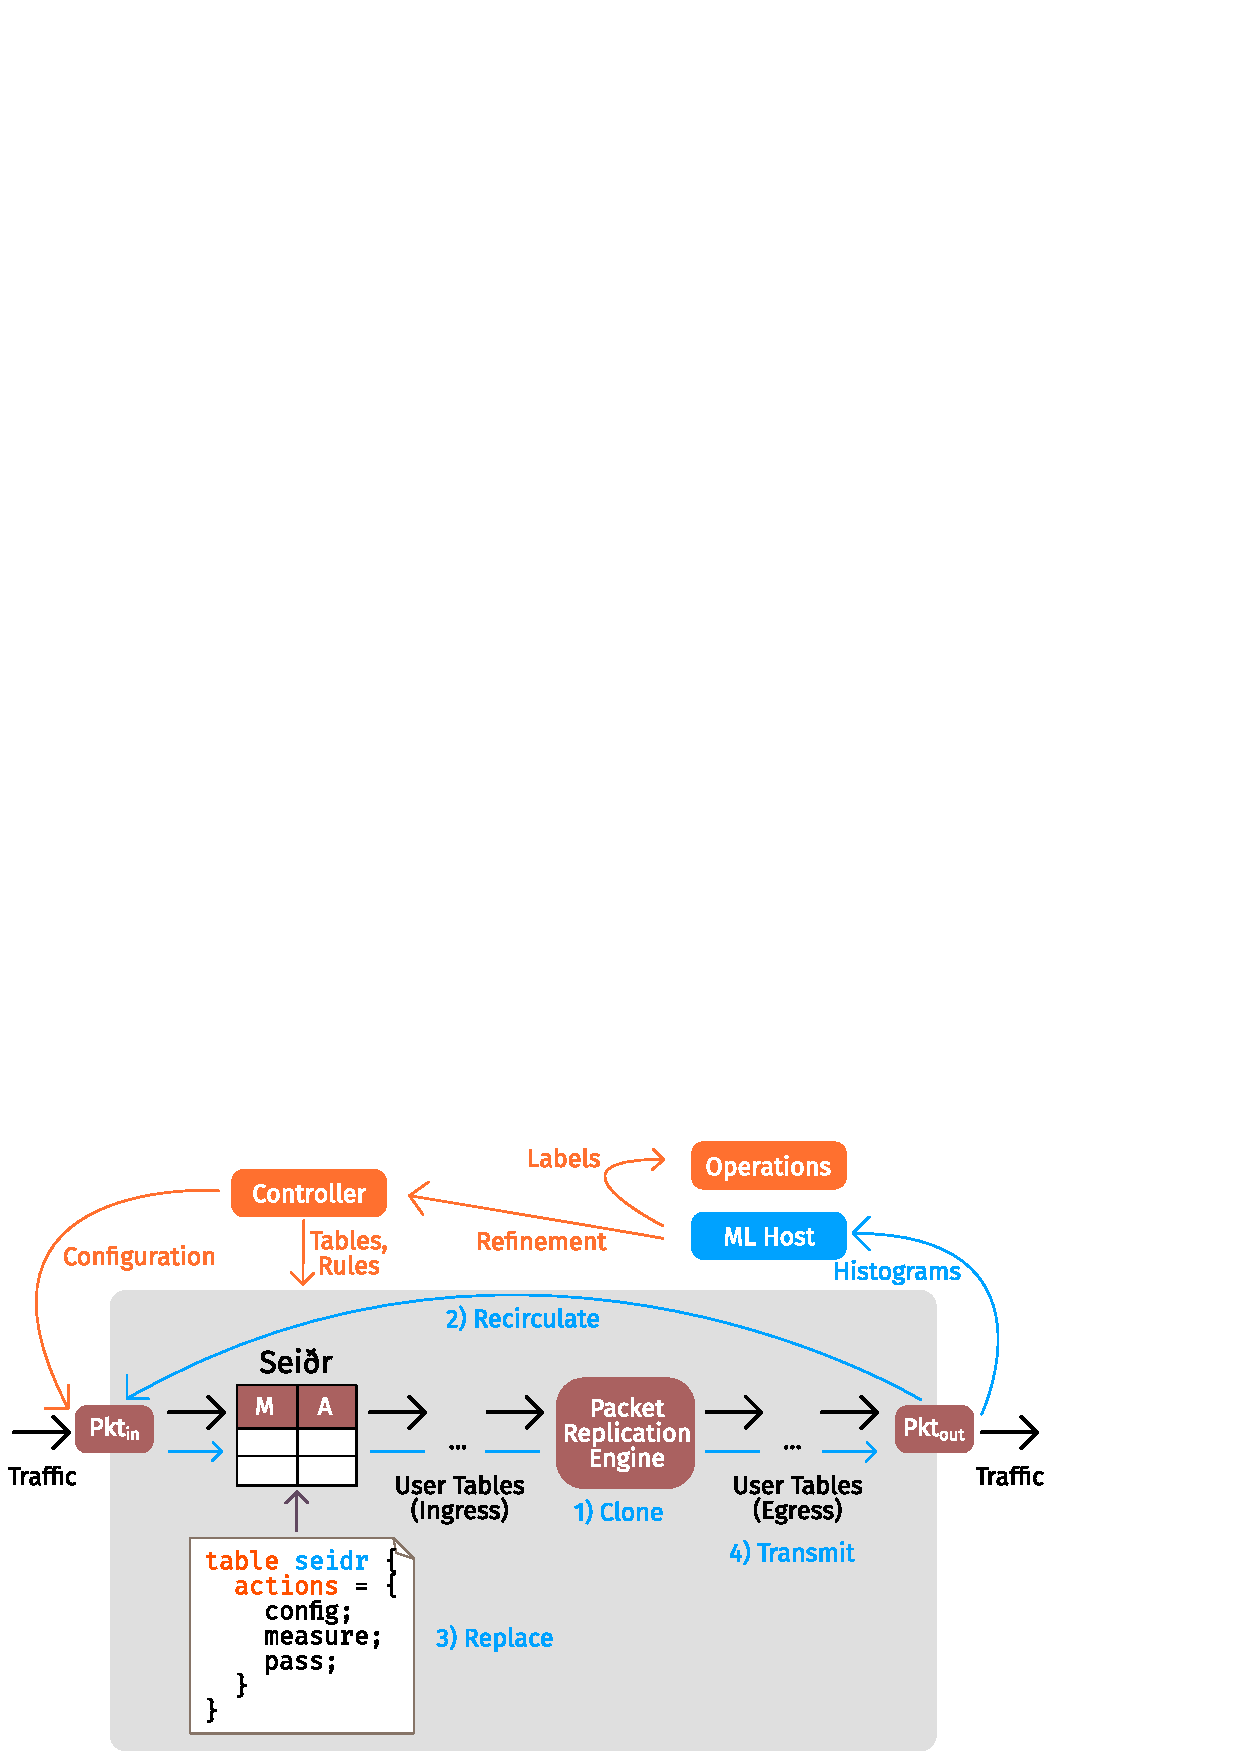
\includegraphics{diagrams/seidr/dp-arch-diagram.pdf}}
    \caption{\seidr{}'s integration with a PSA-compatible~\cite{p4-psa} dataplane.}
    \label{fig:arch}
\end{figure}

% Let's show them a histogram datastructure would look like purely with registers and how would a P4 action populate it - pseudocode or P4 snippet would be nice.

Although packet timing information is useful in understanding network and flow behaviour, without volume or packet rate reduction it is prohibitively expensive for hosts to handle each packet.
Histogramming acts as the \emph{aggregation step} which makes this class of analysis feasible in high-speed networks.
\Cref{fig:arch} demonstrates how \seidr{}, installed as an additional table in any P4 program, records and transmits inter-arrival time histograms.
The format for these histogram packets is outlined in \cref{fig:seidr-headers}; we choose to store individual buckets as \mintinline{rust}{u16}s, and the number of buckets in any histogram is fixed at compile time.
We set this to \num{100} buckets per histogram.
Packets traverse a table which requires \num{3} actions to be implemented:
\begin{enumerate}
    \item \mintinline{rust}{config} reads any matched packets as a \mintinline{rust}{seidr_cfg_t} of type \mintinline{rust}{SET_}\{ \mintinline{rust}{MIN}, \mintinline{rust}{MAX}, \mintinline{rust}{DST}, \mintinline{rust}{SRC}, \mintinline{rust}{LEN} \} by using the P4 parser.
    These update registers \numrange{1}{5} in \cref{tab:registers}, dropping any matched packets.
    
    \item \mintinline{rust}{measure} calculates the inter-arrival time, update per-flow histograms, and transmits finished histograms to the correct host. We describe its operation in \cref{alg:measure}.
    
    \item \mintinline{rust}{pass} ignores packets, and is the default action.
\end{enumerate}
Constructing \seidr{} in this manner allows the control plane to install rules to enable/disable runtime reconfiguration as needed, and to monitor as many or as few flows as desired (\ie, using wildcard rules, or exact matching).

The PSA does not have any mechanisms for generating new packets.
To circumvent this, any packet which would complete a histogram is tagged for cloning at the end of the ingress pipeline, and recirculation at egress (\cref{algline:recirc}).
This truncated copy returns to \seidr{}'s table, where we enable the relevant headers, change L2/3 fields, and write out the histogram contents (\crefrange{algline:rewrite-start}{algline:rewrite-end}).
The P4 deparser outputs the new protocol stack at egress, and transmits the histogram UDP packet into the network.
Event-driven architecture proposals~\cite{DBLP:conf/hotnets/IbanezABM19} may allow a more natural means of packet generation.

\begin{figure}
\centering
\begin{subfigure}{0.45\linewidth}
\centering
\adjustbox{max width = 0.6\linewidth}{
\begin{minipage}{\linewidth}
\begin{minted}[escapeinside=||]{rust}
|\textbf{\textcolor{Keyword}{header}}| seidr_cfg_t {
    bit<8> function;
    bit<144> payload;
}
\end{minted}
\end{minipage}
}
\end{subfigure}
\begin{subfigure}{0.45\linewidth}
\centering
\adjustbox{max width = 0.6\linewidth}{
\begin{minipage}{\linewidth}
\begin{minted}[escapeinside=||]{rust}
|\textbf{\textcolor{Keyword}{header}}| seidr_t {
    bit<128> src_ip;
    bit<128> dst_ip;
    bit<16> src_port;
    bit<16> dst_port;
    bit<16> eth_type;
    bit<BUCKETS * 16> histo;
}
\end{minted}
\end{minipage}
}
\end{subfigure}
\caption{P4 headers for \seidr{} configuration and histograms.}\label{fig:seidr-headers}
\end{figure}

\begin{algorithm}
% \vspace{-0.25cm}
% \DontPrintSemicolon
\KwData{5-tuple, P4 metadata, P4 headers, Registers}
h $\leftarrow$ hash(5-tuple)\;
index $\leftarrow$ BUCKETS * h\;
owner $\leftarrow$ HistoOwner[h]\;
\uIf{metadata.packet\_path = RECIRCULATE}{
    headers.tcp.valid $\leftarrow$ false\label{algline:rewrite-start}\;
    headers.udp.valid $\leftarrow$ true\;
    headers.seidr.valid $\leftarrow$ true\;
    copy 5-tuple into headers.seidr\;
    rewrite headers.ip, headers.udp using HistoSrc/Dest\;
    headers.seidr.histo $\leftarrow$ HistoData[index..]\;
    truncate payload\;
    zero out registers: BucketCount, HistoOwner[h], HistoData[index..]\;\label{algline:rewrite-end}
}
\ElseIf{owner = 0 \textbf{or} owner = 5-tuple}{\label{algline:owner-check}
    HistoOwner[h] $\leftarrow$ 5-tuple\;
    iat $\leftarrow$ LastTimestamp - metadata.mac\_ingress\_time\;
    \If{iat $\ge$ Min \textbf{and} iat $\le$ Max}{
        bucket $\leftarrow$ BUCKETS * (iat - Min) / (Max - Min)\;
        HistoData[index + bucket] $\leftarrow$ HistoData[index + bucket] + 1\;
        BucketCount[h] $\leftarrow$ BucketCount[h] + 1\;
        \If{BucketCount[h] = Len}{
            mark packet for cloning and recirculation\label{algline:recirc}\;
        }
    }
}

\caption{Histogram update and transmission.}\label{alg:measure}
\end{algorithm}

In the event of hash collision (\cref{algline:owner-check}), we ignore packets outside of the tracked flow to ensure that data is accurate.
As later processing and classification directly affect what decisions are made by operators or automatically taken by a policy (possibly leading to incorrect flow limits, QoS, \emph{etc.}), avoiding corruption/cross-contamination of operational data is paramount.
To gain collision resistance, Robin Hood hashing could be used up to a maximum distance in the table, treating a zeroed owner as empty and an illegal source IP as a tombstone value.

\begin{table}
    \centering
    \caption{Register map (Datatype, Amount) for an $h$-bit hash.}
    \resizebox{\linewidth}{!}{\begin{tabular}{@{}ccccccccc@{}}\toprule
        Min & Max & Length & HistoSrc & HistoDest & BucketCount & LastTimestamp & HistoOwner & HistoData \\ \midrule
        \mintinline{rust}{u16} & \mintinline{rust}{u16} & \mintinline{rust}{u16} & \mintinline{rust}{u16 + u128} & \mintinline{rust}{u16 + u128} & \mintinline{rust}{u16} & \mintinline{rust}{u64} & \mintinline{rust}{3 * u16 + 2 * u128} & \mintinline{rust}{BUCKETS * u16} \\
        1 & 1 & 1 & 1 & 1 & $2^h$ & $2^h$ & $2^h$ & $2^h$ \\ \bottomrule
    \end{tabular}}
    \label{tab:registers}
\end{table}

% Basic Logic:
% \begin{itemize}
%     \item table 1: three actions
%     \begin{itemize}
%         \item config: set R1 or R2 (controller installs rule matching a specific port/ip combo)
%         \item measure: take ingress timestamp from metadata, do stuff, write into lasttime, add to bucket and total if within bounds
%         \item pass (default)
%     \end{itemize}
%     \item then pass onto rest of tables
%     \item Why do it this way? can make it all or nothing through control plane.
%     \item How to write and send packet? Same trick as ESNET? (recirc w/ custom metadata to transform pkt)
% \end{itemize}

% ?? NOTE: See PSA \cite{p4-psa} for register format. Some papers, like Dapper, suggest that hash tables should be possible? That would work out very well in our benefit.

% ?? What is configurable? Min, max of the histogramming range

This design allows runtime configuration of all aspects save for the bucket count; at runtime, the only way to increase bucket resolution is to examine a smaller region of IATs.
While in theory this could be configured below a maximum compiled into the firmware, the difficulties introduced in classification/data processing make this infeasible.
Unless using stream-capable classifiers such as LSTMs~\cite{DBLP:journals/neco/HochreiterS97}, changing the input size requires retraining from scratch since new neuron weights must be added and structural properties of the input data change.
Increasing the bucket count requires new firmware installation, as many dataplane P4 implementations cannot allocate variable-length stores due to the lack of a dynamic allocator.

\begin{figure}[t]
    \centering
    \begin{subfigure}[t]{0.49\linewidth}
        \centering
        \resizebox{\linewidth}{!}{\includegraphics{plots/seidr/dt-cubic-1000-app.pdf}}
        \subcaption{TCP Cubic}
        \label{fig:cubic-hist-app}
    \end{subfigure}
    \begin{subfigure}[t]{0.49\linewidth}
        \centering
        \resizebox{\linewidth}{!}{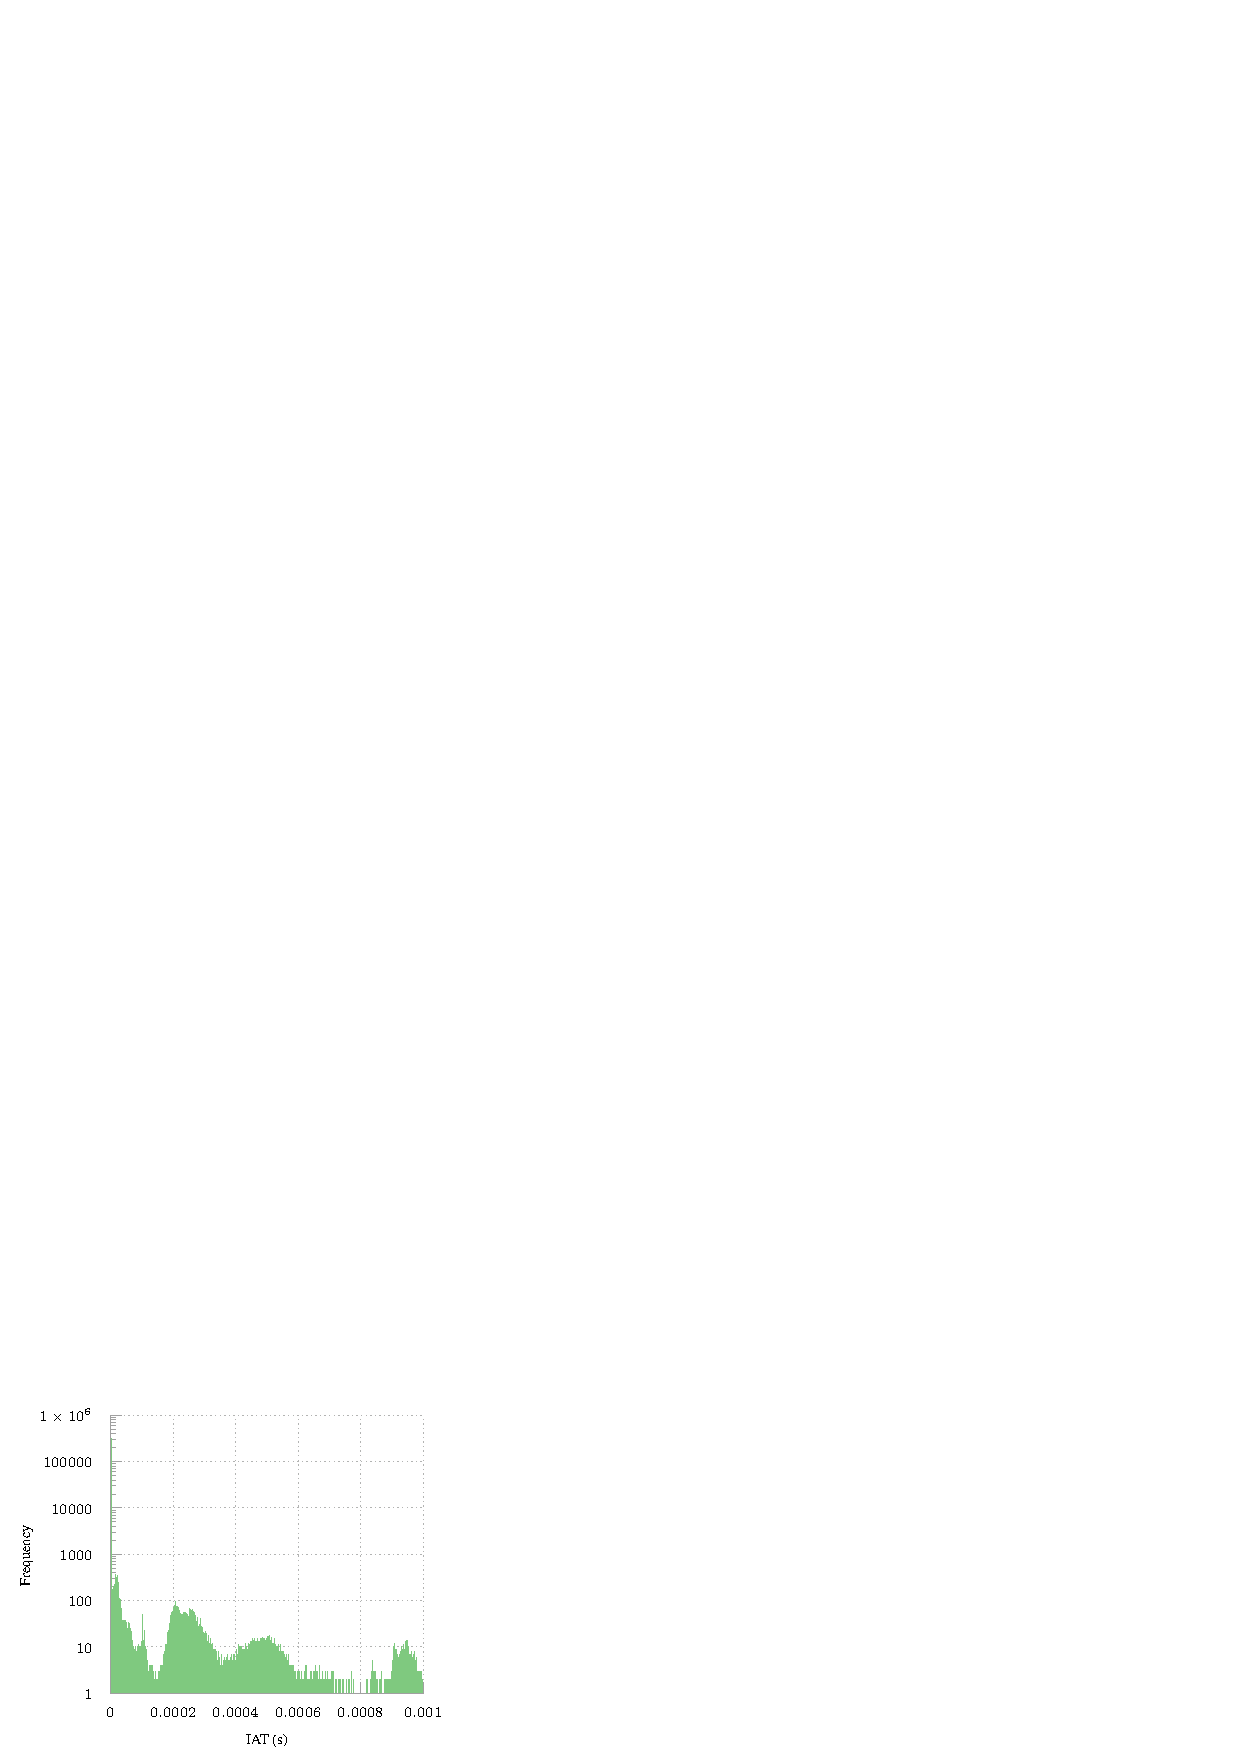
\includegraphics{plots/seidr/dt-bbr-1000-app.pdf}}
        \subcaption{TCP BBR}
        \label{fig:bbr-hist-app}
    \end{subfigure}
    \caption{Example dataplane histograms showing visible differences in inter-arrival times of selected TCP flavours. Our ML solutions are trained to programmatically identify such differences.}
    \label{fig:tcp-hist-app}
\end{figure}

As an example of dataplane-generated histograms, \cref{fig:tcp-hist-app} shows the distribution of inter-arrival times between two TCP congestion control algorithms. The visible differences are programmatically identified using our ML algorithms.

\subsection{Accurate, Precise and High-Resolution Timestamping}

Precise timestamps are critical when detecting temporal properties of flow behaviour, such as microbursts or inferring flow congestion control algorithms.
It is especially important in high speed (\SI{100}{\giga\bit\per\second}) networks, where there can be as little as \SI{6.7}{\nano\second} between packets that need to be analysed.
With a Linux-based software solution (\eg, reading packets from a link with \emph{tcpdump}), the Linux kernel can only provide microsecond-level accuracy with precision in the order of \SI{100}{\micro\second}~\cite{kundel2020p4sta}.
DPDK improves on this, increasing the accuracy to \SI{100}{\nano\second} in the best case~\cite{primorac2017measure}.
However, today's dataplane devices (\eg, Netronome SmartNICs, NetFPGA SUME) allow nanosecond-accurate timestamps to be retrieved from the \emph{Media Access Control} (MAC) modules with a precision of \SI{10}{\nano\second}~\cite{kundel2020p4sta}, a timestamp property \seidr{} relies upon.

% Some platforms provide picosecond-level precision and many solutions allow time synchronisation between multiple devices using the IEEE 1588-2002 (Precision Time Protocol) standard.



\section{TCP congestion control classification}\label{sec:seidr-tcpcc}


% We present an example of first-stage analysis performed for each flow and each packet---stateful TCP analysis.
% This includes numerous metrics which are considered standard when measured at connection endpoints, yet are difficult or invite numerous issues when performed in the network (of which we include a discussion on drawbacks and, curiously, benefits).
% The introduction of accurate timestamps allows us to explore rate-monitoring at a per-packet level, a new view of flow behaviour which may enable flow and hardware characterisation.

% \subsection{Per-Packet Rate Monitoring}

% \begin{figure*}
%     \centering
%     \begin{subfigure}[t]{0.49\linewidth}
%         \centering
%         \resizebox{0.5\linewidth}{!}{
% 	    \begin{tikzpicture}
%     		[packet/.style={draw, fill=uofgsunshine}]
% 		    \node[packet] (p1) {$p_1$: 1500B};
% 		    \node[packet, right= 1cm of p1] (p2) {$p_2$: 800B};
		
% 		    \node at ($(p1.south west) - (0,1)$) (t1) {$t_1$};
% 		    \node at ($(p2.south west) - (0,1)$) (t2) {$t_2$};
		
% 		    \draw[-, dotted] (t1.north)--(p1.south west);
% 		    \draw[-, dotted] (t2.north)--(p2.south west);
		
%     		\draw[<->] (t1.north) -- node[below]{$\mathit{dt}$} (t2.north);
% 	    	\draw[<->] ($(t1.north) + (0,0.2)$) -- node[above]{$s$} ($(t1.north) + (1.8,0.2)$);
% 		    \draw[<->] ($(t1.north) + (1.8,0.2)$) -- node[above]{$g$} ($(t2.north) + (0,0.2)$);
% 	    \end{tikzpicture} 
% 	}
%     \caption{\centering Per-packet rate, visualised. Note that $p_1$ and $p_2$ are not necessarily packets from the same flow.}
%     \label{fig:per-packet-rate}
%     \end{subfigure}
%     \begin{subfigure}[t]{0.49\linewidth}
%     \centering
%     \resizebox{0.9\linewidth}{!}{
% 		\begin{tikzpicture}
% 		[packet/.style={draw, fill=uofgsunshine}]
% 		\node[packet] (p1) {$p_1$: 1500B};
% 		\node[packet, right= 1cm of p1] (p2) {$p_2$: 800B};
% 		\node[right= 1cm of p2] (p3) {...};
% 		\node[packet, right= 1cm of p3] (p4) {$p_{n-1}$: 1500B};
% 		\node[packet, right= 1cm of p4] (p5) {$p_n$: 1500B};
		
% 		\node at ($(p1.south west) - (0,1)$) (t1) {$t_1$};
% 		\node at ($(p2.south west) - (0,1)$) (t2) {$t_2$};
% 		\node at ($(p4.south west) - (0,1)$) (t4) {$t_{n-1}$};
% 		\node at ($(p5.south west) - (0,1)$) (t5) {$t_{n}$};
		
% 		\draw[-, dotted] (t1.north)--(p1.south west);
% 		\draw[-, dotted] (t2.north)--(p2.south west);
% 		\draw[-, dotted] (t4.north)--(p4.south west);
% 		\draw[-, dotted] (t5.north)--(p5.south west);

%         \draw[<->] ($(t2.south) + (0,-0.25)$) -- node[above]{$s$} ($(t2.south) + (6.25,-0.25)$);
%         \draw[<->] ($(t2.south) + (6.25,-0.25)$) -- node[above]{$g$} ($(t5.south) + (0,-0.25)$);
% 		\draw[-, thick] ($(t2.south) - (0,0.5)$) -- node[below]{$W$} ($(t5.south) - (0,0.5)$);
% 		\end{tikzpicture} 
% 	}
%     \caption{\centering Sliding window rate, visualised. Rate estimates are computed using the sizes of the last $W$ packets seen in the current flow. Packets $p_2$ and $p_{n-1}$ belong to the same flow, but $p_n$ is not assumed to.}
%     \label{fig:sliding-window-rate}
%     \end{subfigure}
%     \caption{Comparison of per-packet and sliding window rates. The lengths of packets and inter-packet gaps are not to scale, and are purely demonstrative.}
%     \label{fig:pr-vs-slide}
% \end{figure*}

% Associating each packet with a high-resolution timestamp allows us to introduce the notion of a \emph{per-packet rate}.
% Assuming a packet with size $p$ arrives at time $t_1$ and is followed by another packet (potentially from another flow) which arrives at $t_2$, we measure $\mathit{dt}=t_2-t_1$ for this packet.
% Supposing this first packet spends time $s$ on the wire and assuming that the inter-packet gap $g$ is negligible compared to the length of a packet, then $\mathit{s} = \mathit{dt} - g \approx \mathit{dt}$.
% This packet then has a point rate, $r$:
% \begin{equation}
%     r = \frac{p}{s} \approx \frac{p}{\mathit{dt}}
% \end{equation}
% \Cref{fig:pr-vs-slide} demonstrates how this timing information arises, contrasted with sliding-window rate measurements taken over a longer time period.
% This assumes almost back-to-back traffic, which is realistic in our deployment environment, but to the best of our knowledge no programmable switches expose the timestamp at which the final bit of a packet has been ingested.
% Such a timestamp would allow exact measurement of $s$.

% % ?? we need to be clear about the unintuitive nature of these measurements, include a quick sketch proof which shows that the weighted average of a set of point rates is analytically identical to the sliding window rate/throughput taken over the same period of time.
% While this is an interesting measure to associate with each packet, considering how best to view such rates in aggregate can be counter-intuitive.
% Viewing these rates as time series data reveals interesting distributional characteristics which disagree starkly with our understanding of a flow's rate---for instance, clusters which suggest a different mean.
% Suppose we have a set of measurement indices $C$ with no gaps captured between $t$ and $t'$, partitioned into flows $C = F_1 \cup \dots \cup F_p$.
% To correctly combine a set of point measurements for a flow $F_i$ into an average rate $\overline{r}_{F_i}$, we compute:
% \begin{equation}
%     \overline{r}_{F_i} = \frac{\sum_{a \in F_i} \mathit{dt}_a r_a}{\sum_{c \in C} \mathit{dt}_c}.
% \end{equation}
% In the instance that only one flow is captured (\emph{i.e.}, $F_i = C$), this is a weighted average over point rates, using the $\mathit{dt}$ measured between each packet and the next packet in the same flow as its weight.
% Similarly, this is analytically equivalent to the sliding-window rate measured over the same set of packets:
% \begin{equation}
%     \frac{\sum_{a \in F_i} \mathit{dt}_a r_a}{\sum_{a \in F_i} \mathit{dt}_a} \simeq \frac{\sum_{a \in F_i} p_a}{t' - t}.
% \end{equation}
% % \begin{proof}
% % Given a set of contiguous measurements from the same flow $S \subseteq \mathbb{Z}$, admitting $p_s$, $r_s$, $\mathit{IAT}_s$ and $t_s$, the weighted average of point rates is then
% % $$
% % \overline{r}_S = \frac{\sum_{s \in S} \mathit{IAT}_s r_s}{\sum_{s \in S} \mathit{IAT}_s}
% % $$
% % The sliding-window average:
% % $$
% % \overline{r}_S = \frac{\sum_{s \in S} \mathit{IAT}_s r_s}{\sum_{s \in S} \mathit{IAT}_s}
% % $$
% % \end{proof}

% We assume that inter-packet gaps will be negligible (\emph{i.e.}, that the link is never in a state of very low utilisation), due to typically high utilisation on a WAN.
% % Similarly, we need to discuss the effects of selective monitoring or an abundance of UDP/ICMP traffic (which will distort $dt$s).
% However, this assumption can be distorted if selective TCP flow monitoring is used, or if UDP/ICMP traffic is overabundant; both these scenarios create larger gaps between TCP packets of interest, inflating $g$ to the point where it is comparable in size to $s$.
% This has an impact on our notion of per-packet rates, but not inter-arrival times or other such dependent metrics.
% The effect is small on sliding window rates, particularly at larger window sizes.
% ?? Justify. On paper, it looked like error term was O(1/n), O(g) for an n packet window.


% \section{Inter-Arrival Time}

% Having assigned each packet in a flow with a nanosecond-accurate timestamp ?? tbc

\Cref{fig:tcp-hist-app} suggests that a notable use-case for this type of measurement is \emph{congestion control algorithm} (CCA) detection.
In a TCP connection, each machine is free to choose the CCA it uses to send bytes, and thus how it responds to network congestion signals.
This choice is local, and so is invisible to the other machine (and the network).
In datacentre networks, operators choose these to ensure optimal behaviour.
In a transit network or large WAN however, these hosts (and thus the CCAs in use) are outside the control of network operators, which introduces difficulties when CCA interactions lead to \emph{unfairness}.
Consider the recent (and widespread) introduction of \emph{TCP BBR}~\parencite{DBLP:journals/queue/CardwellCGYJ16}.
\emph{BBR} is a delay/model-based CCA which converges on a fair share of bottleneck bandwidth by reducing its rate if the round-trip time increases, while periodically attempting to increase send rate to account for path/load changes.
However, \emph{BBR} traffic can consume \SI{40}{\percent} of link capacity when multiplexed with loss-based CCAs, regardless of the number of competing flows~\parencite{DBLP:conf/imc/WareMSS19}. 
When ensuring fair transit to all flows, this is hardly a desirable outcome; in fact, it's one which may frustrate clients or violate SLAs.

A curious property of \emph{BBR}'s algorithm which sets it apart from other variants is that packet transmission is \emph{timer-based}.
\texttt{send(packet)}, as defined in the canonical algorithm, asks that on transmission of a packet, the sender should wait for the estimated time that packet would take to reach the recipient.
For instance, at an estimated bottleneck bandwidth of \SI{8}{\mega\bit\per\second}, a \SI{1024}{\kilo\byte} packet would hold back the next packet in the flow until \SI{976.6}{\micro\second} had elapsed.
When packet sizes remain similar this causes strongly periodic behaviour, while mode switches in the \emph{BBR} algorithm cause these periodic bands to shift up or down accordingly.
This effect is stronger than in existing loss- and delay-based algorithms which remain intrinsically tied to the notion of a congestion window (where release of buffered packets follows the receipt of ACK messages).
As a result, timing behaviour of past CCAs may be influenced by (the lack of) packet pacing, periodic components might be made noisier by jitter along the return path, or the behaviour of the receiver might add further noise.

This high-level analysis of \emph{BBR} gives us a strong feature to use as the basis for classification: the \emph{inter-arrival times} (IATs) for each packet in a flow.
We have two options for processing this for classification: we may use a compressed, fixed-size representation such as histograms to capture the aggregate distribution, or we may attempt to capture structural behaviour by using a variable-length stream of IATs.
In many networks, the data and packet rate reduction offered by the former is required to make this possible.
Indeed, in-switch aggregation has seen great success in aiding ML for training~\parencite{DBLP:conf/isca/LiLYCSH19}, and direct execution~\parencite{DBLP:conf/hotnets/XiongZ19}.
We make use of the following standard classification algorithms on a fixed-size representation to attempt to single out the CCA in use:

\begin{itemize}
    \item \emph{$k$-Nearest Neighbours ($k$-NN)}. A simple and well-understood classifier which assigns labels based on the closest members of the training corpus (\ie, by the $L_2$ metric). Linear memory cost in amount of training data, and no training cost other than loading all data points, but capable of learning complex decision boundaries on fixed-length input.
    
    \item \emph{Convolutional Neural Networks (CNNs)}. A neural network approach which learns convolution kernels to classify fixed-length data, particularly when recognising spatial features. Memory cost is fixed for a given architecture irrespective of training data, with a high training cost.
\end{itemize}
% \fakepara{Long Short-Term Memory~\parencite{DBLP:journals/neco/HochreiterS97} units (LSTMs)} A class of recurrent neural network used for stream classification, forecasting, and prediction of variable-length data. Memory cost is fixed, with longer training times (and more data required) than similarly sized CNNs.
% Of these, we apply $k$-NN and CNNs to histograms of packet IATs, and LSTMS to raw IAT streams.

When examining $k$-NN classifiers, we measured accuracy across choices of $k \in \left[2, 8\right]$.
We found $k=2$ to be the most effective choice with our input data using the $L_2$ metric.
Our CNN architecture is described in \cref{tab:cnn-arch}, using ReLu activation and $1 \times 1$ stride in convolutional layers unless stated otherwise.
Training occurred over 5 epochs using the Adam optimiser with categorical cross-entropy as a loss metric, and a batch size of \num{64} histograms (\num{8} for full sequences due to the smaller data volume).
For \emph{BBR vs.\ Cubic}, the complete model consists of \num{104898} 32-bit floating-point parameters (\SI{409.76}{\kibi\byte}), while the full classification task adds a further \num{130} parameters (\SI{0.51}{\kibi\byte}).

\begin{table}
    \centering
    \caption{CNN architecture for \num{100}-entry histograms.}
    \resizebox{0.7\linewidth}{!}{\begin{tabular}{@{}cccc@{}}\toprule
        Layer & Nodes/Filters & Filter Size & Output Dimension \\ \midrule
        Conv2D & 32 & $(3 \times 1)$ & $(98 \times 1 \times 32)$ \\
        MaxPool & --- & $(2 \times 1)$ & $(49 \times 1 \times 32)$ \\
        Conv2D & 64 & $(3 \times 1)$ & $(47 \times 1 \times 64)$ \\
        MaxPool & --- & $(2 \times 1)$ & $(23 \times 1 \times 64)$ \\
        Conv2D & 64 & $(3 \times 1)$ & $(21 \times 1 \times 64)$ \\
        Flatten & --- & --- & \num{1344} \\
        Dense & 64 & --- & \num{64} \\
        Dense (Softmax) & $n_\mathit{classes}$ & --- & $n_\mathit{classes}$ \\
        \bottomrule
    \end{tabular}}
    \label{tab:cnn-arch}
\end{table}


\section{Evaluation}\label{sec:seidr-evaluation}
%Traffic is played back from hosts via Tcpreplay at a bandwidth assigned uniformly from a `good' or `bad' distribution, each using the same pcap file with source and destination IP addresses rewritten.

This work is most naturally compared against Marl, introduced by \textcite{DBLP:journals/eaai/MalialisK15}, the state-of-the-art in \gls{acr:rl}-based \gls{acr:ddos} prevention.
We are most interested in seeing how their approach contrasts with the new agent designs across different topologies and workloads.
Different network environments will also impose different levels of host density, where popular web servers may have orders of magnitude more clients than egress points from their network---I aim to show how these characteristics affect performance and learning rate.
Marl is known to outperform the AIMD~\parencite{DBLP:journals/ton/YauLLY05} strategy, yet the state of the art has long since moved on.
To paint a more current picture, I compare this work against an effective modern approach, \emph{SPIFFY}~\parencite{DBLP:conf/ndss/KangGS16}.
SPIFFY tests a proportion of flows by routing them through an alternate path with higher bandwidth, observing how their speed changes some time later.
This comparison lets us position our new agent designs against the state of the art, observing that SPIFFY has a similar mode of interaction to \gls{acr:rl}-based systems (taking action, observing an effect, and acting once again) and does not rely on protocol characteristics or signatures.
In reimplementing SPIFFY, I make the simplifying assumption that a suitable unused path exists (with identical bandwidth to the server's link).
\qty{10}{\percent} of active flows were tested at a time (according to the authors' observation that there is a factor of \qty{10}{\times} difference between the ideal and achieved bandwidth expansion), excluding flows below \qty{50}{\kilo\bit\per\second} and requiring a \qty{3}{\times} expansion from legitimate flows, making a judgement after \qty{5}{\second}.

To test this, I made use of both traffic models introduced in \cref{sec:a-new-normal} (Opus and \gls{acr:tcp}), both topologies discussed below (1-dest vs.\ Fat-Tree), and vary the amount of hosts typically communicating over each agent's ingress/egress node.
Additionally, these new models were evaluated in multi-agent mode (\emph{separate}, no model sharing), and in single-agent mode (\emph{single}, zero-cost perfect information sharing).
In each case, the algorithm's performance was averaged over \num{10} episodes of length \num{10000} timesteps (setting each agent's $\wvec{}=\mathbf{0}$ between episodes).
Host allocations at the beginning of each episode were generated pseudorandomly to ensure fairness between episodes---a host is malicious with probability $\operatorname{P}\left(\mathit{malicious}\right)$, and is benign otherwise.
Benign hosts generate traffic according to either \cref{sec:tcp-http-traffic-model,sec:udp-opus-traffic-model} depending on the experiment, while malicious hosts generate traffic as described in \cref{sec:attack-traffic-model} (both at experiment-dependent rates).

All experiments were executed on Ubuntu 18.04.2 LTS (GNU/Linux 4.4.3-040403-generic x86\_64), using an Intel Core i7-6700K (\qtyproduct[product-units=single]{4 x 4.2}{\giga\hertz}) which had \SI{32}{\gibi\byte} of \gls{acr:ram}.
%All code underpinning these findings is available on a public repository\footnote{\url{https://github.com/FelixMcFelix/rln-dc-ddos-paper}}.
%All code underpinning these findings is available on a public repository.\footnote{Private until publication.}

\subsection{Single destination}\label{sec:single-dest}
%?? Move description of tree topol to here.
The network is tree-structured, where one server $s$ connects through a dedicated switch to $k$ team leader switches, each connected to $\ell$ intermediate switches, which in turn each connect to $m$ egress switches.
We then have $N_{\mathit{hosts}} = k \ell m n$.
\Cref{fig:marl-topol} demonstrates this.
%Although \citeauthor{DBLP:journals/ccr/MahajanBFIPS02a}, the originators of this topology, make it clear that it exists as a fairly unrepresentative example \cite{DBLP:journals/ccr/MahajanBFIPS02a}, it remains the case that such a network topology allows for functional testing, and indeed is illustrative of one way in which attack traffic might aggregate in the network.
%It is hard, however, to argue its relevance to specific classes of victim or to reason about the interactions it might have with dependent applications.
%We aim to address this through \cref{sec:performance-in-an-emulated-environment}.
The network topology was configured using $k=2$ teams, $\ell=3$ intermediate nodes per team, $m=2$ agents per intermediate node, and $n \in \{2, 4, 8, 16\}$ hosts per learner.
This is a slight simplification of \Textcite{DBLP:journals/eaai/MalialisK15}'s \textquote{online} experiment, choosing fewer teams but remaining as a single server with a fan-out network.
%The algorithm parameters were set at $\gamma=0$ (leading to opportunistic behaviour), $\alpha=0.05$, having linearly annealed $\epsilon=0.2 \rightarrow 0$ by $t=3000$.
%Benign and malicious hosts uploaded between \SIrange{0}{1}{\mega\bit\per\second} and \SIrange{2.5}{6}{\mega\bit\per\second} respectively, and hosts were redrawn at each episode's start with $\operatorname{P}(\mathit{malicious})=0.4$.
%$U_s$  $k \ell mn+2$ \si{\mega\bit\per\second}.
%The performance of each choice of $n$ was averaged over \num{10} episodes of length \num{10000} timesteps (setting each agent's $\wvec{}=\bm{0}$ between episodes).
%Host allocations were generated pseudorandomly to ensure fairness between choices of $n$.
%These parameter choices match those of the original study to enable direct comparison, and are (to the best of our knowledge) arbitrary, but we justify our range of $n$ as capturing increasing scales of host activity.

\begin{figure}
	\centering
	\resizebox{0.9\linewidth}{!}{\begin{tikzpicture}[
	texts/.style = {text=black},
	labeltexts/.style = {text=uofgsandstone},
	treeline/.style = {draw=uofgburgundy},
	treenode/.style = {texts, circle, centered, fill=white, treeline},
	load/.style = {fill=uofgcobalt},
	loadhide/.style = {fill=uofgcobalt!40!white},
	external/.style = {fill=uofgrust},
	externalhide/.style = {fill=uofgrust!40!white},
	hideline/.style = {draw=uofgsandstone!40!white},
	hidenode/.style = {treenode, hideline},
	grow'=right
]
	\node[treenode, label={[texts]above:Server}] (root) {}
	child [treeline] { node [treenode, label={[texts]above:Core}] (sswitch) {}
		child [treeline] { node [treenode, label={[texts]above:Leader}] (teaml) {} 
			child [treeline] { node [treenode, label={[texts]above:Intermediate}] (inter) {}
				child [treeline] { node [treenode, load, label={[texts]above:Agent/Egress}] (agent) {}
					child [treeline] { node [treenode, external] (extern) {}
						child [treeline] { node [treenode, external, label={[texts]above:Host}] (host) {} }
						child [hideline] { node [hidenode, externalhide] (endhost) {} }
					}
				}
				child [hideline] { node [hidenode, loadhide] (endagent) {} }
			}
			child [hideline] { node [hidenode] (endinter) {} }
		}
		child [hideline] { node [hidenode] (endteaml) {} }
		edge from parent
		node[below, labeltexts] {$U_s$}
	};
	
	%\draw[-] (teaml) -- (endteaml);
	\node [labeltexts] (kdots) at ($(teaml)!0.5!(endteaml)$) {$\rvdots$};
	\node [labeltexts, right = -0.1cm of kdots] {$k$};
	\node [labeltexts] (ldots) at ($(inter)!0.5!(endinter)$) {$\rvdots$};
	\node [labeltexts, right = -0.1cm of ldots] {$\ell$};
	\node [labeltexts] (mdots) at ($(agent)!0.5!(endagent)$) {$\rvdots$};
	\node [labeltexts, right = -0.1cm of mdots] {$m$};
	\node [labeltexts] (ndots) at ($(host)!0.5!(endhost)$) {$\rvdots$};
	\node [labeltexts, right = -0.1cm of ndots] {$n$};
\end{tikzpicture}}
	\caption[Tree-structured network topology diagram for evaluating a single-destination network.]{
		Network topology diagram, showing how the server and its core switch's $k$ teams are structured, with $\ell$ intermediate routers per team, connected to $m$ agents which each moderate $n$ hosts beyond a single external switch.
		%	Empty nodes are considered to be internal.
		Red nodes are external, and each blue node hosts an agent.
		\label{fig:marl-topol}
	}
\end{figure}

\subsection{Multiple destinations}
The previous topology allows for direct comparison against the state-of-the-art, and indeed is illustrative of one way in which attack traffic might aggregate in the network.
It is hard, however, to argue its relevance to specific classes of victim or to reason about the interactions it might have with dependent applications.
In contrast, the fat-tree topology~\parencite{DBLP:conf/sigcomm/Al-FaresLV08} sees regular use in real-world data centres and scales well horizontally.
%?? Come up with description of fat-tree (multi-dest) topol.
%?? Why fat tree? regularly appears in modern datacentres.
%?? $k=4$ fat-tree , with one pod hosting two servers $s_0,s_1$.
We use a $k=4$ fat-tree, with one pod hosting two servers $s_0$ and $s_1$.
$n$ external hosts connect through each core switch (where agents are hosted), and communicate with $s_0, s_1$ uniformly randomly.
Both servers host identical services.
We set $n \in \{6, 12, 24, 48\}$ hosts per learner (keeping $N_{\mathit{hosts}}$ identical to each tier of the single-host topology), and restrict $U_{s_0} = U_{s_1} = U_s / 2$.

\subsection{Parameters}
The algorithm parameters were set at $\alpha=0.05$, linearly annealing $\epsilon=$ \num{0.2} $\rightarrow$ 0 by $t=$~\num{3000} in the case of Marl (\num{8000} actions per agent in the \emph{Instant/Guarded} models).

Benign hosts each occupied \qtyrange{0}{1}{\mega\bit\per\second}, and hosts were redrawn at each episode's start with $\operatorname{P}(\mathit{malicious})=$~\num{0.4}.
%The original introduction of this approach to direct-control reinforcement learning as introduced by \textcite{DBLP:journals/eaai/MalialisK15} fails to consider key cases: the absence of a suitable heuristic classifier $g(\cdot)$, disjoint ranges of traffic distribution (i.e., the presence of benign heavy-hitters), the accurate simulation of TCP-like behaviour (and its effects on collateral damage), and high densities of hosts at egress points.
%?? Why? ...
%Of these, the latter two are most deserving of a closer investigation, as they have stronger implications for wide-scale deployment.
%These are important issues, particularly when we consider real-world deployment.
%Heuristic estimates of traffic legitimacy come with computational cost and couple the reward function to the accuracy of the estimator, hosts often show diversity in their own traffic patterns (perhaps being multi-modal), and it is known that TCP is the most used transport protocol for Internet traffic \cite{DBLP:conf/saint/ZhangDJC09}.
%?? NEED TO VERIFY VOLUME OF CONGESTION-AWARE PROTOCOLS
Malicious hosts each sent \qtyrange{2.5}{6}{\mega\bit\per\second} when attacking \gls{acr:udp} traffic, though this was increased to \qtyrange{4}{7}{\mega\bit\per\second} when using \gls{acr:tcp}-like traffic (to meaningfully impact benign flows).
Given $n$ and $\operatorname{P}(\mathit{malicious})$, we see an expected malicious bandwidth \numrange{1.27}{1.87} and \qtyrange{2.03}{2.18}{\times} $U_s$ respectively.
%The expected fraction of $U_s$ consumed by each host is \SI{21.5}{\percent} for $n=2$, and \SI{2.84}{\percent} for $n=16$.
For these choices of $n$ in both topologies, we observe $N_{\mathit{hosts}} \in \left\{24, 48, 96, 192\right\}$, and an expected number of malicious hosts $\mathbb{E}\left[N_{\mathit{attackers}}\right] \in \left\{9.6, 19.2, 38.4, 76.8\right\}$.
For the largest choice of $n$, we see an expected total attack traffic $\mathbb{E}\left[V_{\mathit{attack}}\right] =$ \qtylist{334.05;422.4}{\mega\bit\per\second} for Opus and \gls{acr:http} traffic respectively.

$U_s$ was fixed at $N_{\mathit{hosts}}+2$ \unit{\mega\bit\per\second} (to account for burstiness), and each link had a delay of \qty{10}{\milli\second}.
All links had unbounded capacity, save for each server-switch.
These parameters match those of the original study to enable direct comparison, and many are (to the best of our knowledge) arbitrary, but I justify the range of $n$ as capturing increasing scales of host activity.

% \section{Related Work}\label{sec:related}
% %?? Try and compare my work here when possible?

\fakepara{DDoS Prevention}
\Textcite{DBLP:conf/lcn/BragaMP10} examine the detection of flooding DDoS attacks through \emph{self-organising maps}, using SDN to gather statistics effectively.
Many of their features aren't overly relevant, as their focus is not active defence or discovering \emph{which} hosts contribute to an attack.
%?? Actually talk about Marl (???) to appease reviewer \#1.
The closest available approach within this field is that of \textcite{DBLP:journals/eaai/MalialisK15} (whom we have positioned our work against), and their contribution in applying RL to the task of intrusion prevention is significant: their work helps to show the viability of live, adaptive, feedback-loop-like control of the network to detect and prevent DDoS attacks.
They create a tree overlay topology (subdivided into teams), where each agent applies packet drop to \emph{all} flows inbound to a protected server.
%?? Recap their flaws, since they've been cut form every other aspect.
Our results show that their technique underperforms at high host density and when congestion-aware traffic dominates---that their results do not demonstrate this suggests an evaluation driven purely by traces (rather than live application dynamics).

\emph{SPIFFY} \cite{DBLP:conf/ndss/KangGS16} aims to remedy transit-link attacks by observing how flows from each source respond to a sudden increase in available bandwidth.
\Citeauthor{DBLP:conf/ndss/KangGS16} realise that bots participating in an attack are often unable to match this bandwidth expansion (having already saturated the capacity of their outbound links), while legitimate flows typically speed up to match the new fair-share rate.
%Attackers must either be detected or reduce the throughput of each bot, increasing the cost of launching an attack.
%Unlike our approach (and due to the class of attacks it is designed to defend against), SPIFFY is intended to be deployed within ASes, although .
A weakness of their approach is that computing a route to measure bandwidth expansion on real networks can be costly (up to \SI{14}{\second} for the Cogent topology), and that the low expansion factors in real network can require more ``rounds'' of filtering.
By contrast, our approach takes a constant time to compute an action for a flow regardless of topology size.
Their assumptions about traffic response to such bandwidth expansion do not hold for constant bitrate flows (e.g., VoIP) and may not extend to HTTP DASH flows, both of which make up a sizeable proportion of network traffic.

\emph{Athena} \cite{DBLP:conf/dsn/LeeKSPY17} is a generalised SDN framework for intrusion detection, but has shown the use of a \emph{k-nearest neighbours} classifier to detect individual attack flows.
Although heavyweight (and proven to be effective compared with \textcite{DBLP:conf/lcn/BragaMP10}), their comparison against SPIFFY lacks the quantitative evidence required to understand how the system compares.
\Textcite{DBLP:conf/sp/SmithS18} use AS-level routing to tackle both transit-link and flooding-based attacks.
This view is taken due to the perceived cost of per-stream classification and inherent sensitivity to adversarial examples.
The approach is creative, relying upon BGP \emph{fraudulent route reverse poisoning} to preserve traffic to a target AS, but unlike SPIFFY the approach doesn't actually \emph{remove} the congestion.
Because of this, flooding-based attacks aren't fully alleviated.

%?? Abuses of RL 
\fakepara{RL in Networks}
Earnest, well-considered application of RL towards the challenge of intrusion prevention has seen comparatively little examination.
Past work treats the paradigm as a traditional classifier for anomaly detection \cite{shamshirband2014anomaly} and DDoS prevention \cite{DBLP:conf/mates/ServinK08}.
Given that the main strengths of RL techniques are the ability to control ongoing interaction and adapt by observing the concrete effects of actions, such works don't apply the rich literature on the subject to its fullest potential.

For categorising how RL fits into solving problems, we label works as direct- or indirect-control RL.
A \emph{direct-control} RL problem is one where the RL agent(s) learn optimal control over a set of actions as the \emph{primary} defence or decision-maker---requiring measurements, reward functions and action sets tailored for this purpose.
%We feel there is a shortage of work in this category at present, at least in the field of networks.
To date, the best-fitting example we have encountered is that of \textcite{DBLP:journals/eaai/MalialisK15}.
An \emph{indirect-control} RL problem is one where agents act in service to \emph{another technique} responsible for decision-making, optimising or generalising aspects of its operation beyond that of hand-coded heuristics.
A past example includes learning when best to share knowledge between \emph{hidden Markov model} anomaly detectors \cite{DBLP:conf/paisi/XuSH07}.
%The position of this work is weakened by its reliance on the problematic `DARPA99' dataset \cite{DARPA-IDD, DBLP:conf/cisda/TavallaeeBLG09, DBLP:conf/sp/SommerP10}, but the idea itself is well-treated and this acts as a driver for improvements in this direction.
This work is weakened by its reliance on the problematic `DARPA99' dataset \cite{DBLP:conf/sp/SommerP10}, but the idea itself is well-treated.
Outside of intrusion detection, there has been growing interest in the use of RL in data-driven networking, such as for intra-AS route optimisation \cite{DBLP:conf/hotnets/ValadarskySST17} and resource-constrained process allocation \cite{DBLP:conf/hotnets/MaoAMK16}.
\textcite{DBLP:conf/sigcomm/MaoNA17} employ client-side observations of network state and video performance with RL to optimise bitrate selection for multimedia streaming.
\emph{AuTO} \cite{DBLP:conf/sigcomm/ChenL0L18} employs deep RL to perform traffic optimisation.
Crucially, they find that the vast majority of flows are short-lived, requiring effective decisions in less than a millisecond.
To overcome the high latency of action computation via a neural network, two agents are trained, handling aspects of short and long flows respectively.
The first learns to optimise the flow size thresholds to demarcate long and short flows; these short flows are routed by ECMP.
The second agent makes bespoke decisions about routing, prioritisation etc.\ for each of the remaining long flows.


\section{Summary}\label{sec:seidr-conclustion}
We have presented \seidr{}, a dataplane assisted flow classification solution that can be used to detect fine-grained temporal flow behaviour. We have shown a PSA-compliant way to implement in-network data aggregation in the form of histograms, while using nanosecond-precision timestamping. Our in-network generated histogram datastructure (\eg, on per-flow packet inter-arrival times) has been presented as the input for various ML algorithms, including CNN and $k$-NN. We have shown with our extensive evaluation that \seidr{} can successfully tell apart TCP CCAs, in particular, it identifies BBR from its predecessors with over \SIrange{88}{96}{\percent} accuracy, while only consuming a maximum \SI{15.5}{\mebi\byte} of dataplane memory. We presented the trade-offs between training and inference times, memory requirements, and accuracy in the context of CNN and $k$-NN classifiers and shown that \seidr{} outperforms prior work by increasing classification accuracy on novel TCP CCAs, providing the ability to classify at very high traffic rates (in the order of \SI{10}{\tera\bit\per\second}).
Furthermore, we have identified a key temporal property of \emph{BBR} which allows its easy detection among other flows.
In the future, we aim to examine the use of \seidr{} towards microburst detection and diagnosis~\cite{DBLP:conf/sigcomm/ChenFKRR18} and for the identification of \emph{BBR}-like temporal properties of emerging UDP-based congestion-aware protocols, such as \emph{QUIC}.%~\cite{DBLP:conf/sigcomm/LangleyRWVKZYKS17}.

?? Through this chapter, we have discussed ..., lending credence to one of the claims in my thesis statement: \superrecallthesis{3}


% -----------------------------------------------------------------------------

%\part{Appendices}
\appendix
\renewcommand\chaptername{Appendix}

\chapter{Protocol Trends in CAIDA Traces}
\label{adx:caida-traffic}

Detail and explain the stuff in that repo here.\gls{acr:caida}~\parencite{caida-2018-passive}

\chapter{Opus VoIP Traffic Capture and Generation}\label{adx:opus-traffic}
To provide a realistic model of normal congestion-unaware traffic to properly evaluate the work in \cref{chap:ddos-rl}, I passively measured \gls{acr:voip} traffic generated by users of the Discord~\parencite{discord} online chat service to acquire reasonable traces and then generate appropriately similar traffic.
Discord allows text, voice and streaming video conversation between users---the latter two allow real-time communication over \gls{acr:udp}.
I am interested here in voice, which is effectively \gls{acr:cbr} and congestion-unaware, but is easily accessible by bot users (unlike video).

\gls{acr:voip} application traffic has interesting characteristics.
Client$\rightarrow$server flows contain an audio stream mixed with in-band and out-of-band control traffic.
Audio streams are encoded at a target bitrate (e.g., \qty{96}{\kilo\bit\per\second}) and divided into individual packets to provide continuous delivery of traffic---these are usually relatively large ($\sim$\qty{20}{\milli\second}) to reduce packet transport overhead, but small enough to minimise the impact of packet losses.
Due to this real-time requirement, audio packet arrivals and transmissions are then highly periodic.
There are other interesting dynamics, aside from the trivial observation that flows won't react substantially to lost packets.
In Discord's architecture (and I suspect in the general case nowadays to achieve better and more consistent \gls{acr:qoe}), \emph{all} packets are sent to a single \gls{acr:turn} server~\parencite{rfc8656}, which relays them between users to ensure connectivity (as opposed to, say, peer-to-peer session links).
This causes inbound \gls{acr:rtp} packets to fan out to all other participants in a call, leading to a moderate amplification factor.

%?? Also interesting per-server dynamics. TURN servers, fan in/out -- similarity to attacks in some respects? (i.e., \gls{acr:turn}~\parencite{rfc8656} server amplifies.)

Sadly, it is insufficient to just encode arbitrary audio at a voice channel's supposed bitrate and then divide that into fixed-size packets.
The exact size of each packet depends on the carried content, but tends in the long term towards \gls{acr:cbr} for speech or music.
Silent frames are, of course, the smallest to encode (e.g., \qty{5}{\byte} for the Opus codec).
Smaller signal-dependent variations aside, since users tend to converse with each other they typically speak in bursts of various lengths rather than continuously, and can cease sending packets during these times to save bandwidth.
Obviously, this leads to burstier traffic than simply taking the expected link occupation over each user's stream.
Moreover, the duration of individual voice sessions and number of recipients also play a part in how traffic is fanned out at the \gls{acr:turn} server, and to whom.

From the above, we have quite a few factors which affect both client$\rightarrow$server and server$\rightarrow$client behaviour.
At the time I was designing the evaluation for \cref{chap:ddos-rl}, I couldn't find conclusive studies on \gls{acr:voip} traffic which would be at all useful in modelling these sorts of dynamics---and still haven't quite seen any works which fill the same niche.
This appendix describes my methodology for capturing and generating somewhat simplified variants of these flows---i.e., discounting control traffic and shared sessions to minimise out-of-band coordination.

%?? WHy all this? Couldn't find a good generator.
%
%?? Problem description: Discord \gls{acr:voip} flows are \gls{acr:cbr} while speaking (bitrate is chosen per voice channel, not adaptive in this circumstance). 

%?? Highly periodic

\section{Voice session behaviour}
Discord's \gls{acr:voip} sessions target a preset bitrate per voice channel chosen by that server's administrators---\qtyrange{8}{96}{\kilo\bit\per\second} on free servers\sidenote{\qtylist{128;256;384}{\kilo\bit\per\second} are offered to paying users. This only affects client behaviour: the \gls{acr:turn} server is not stringent enough to block or re-encode voice data sent by bots or custom clients.}, defaulting to \qty{64}{\kilo\bit\per\second}.
Clients connect by requesting session IDs and keys over the main WebSocket \gls{acr:api}, which are used to open another WebSocket session for voice control traffic.
This includes negotiating the cryptographic tag scheme, and receiving an \gls{acr:rtp} \gls{acr:ssrc}, URL and port for a \gls{acr:udp} \gls{acr:turn} server.
Connection then proceeds to make use of WebRTC (web browser users) or vanilla \gls{acr:rtp}: in the latter case, explicit \gls{acr:nat} hole punching is performed.
This WebSocket session is maintained over the call's lifetime to provide information about other users and exchange periodic heartbeat messages.

% \gls{acr:voip} flows are \gls{acr:cbr} while speaking (bitrate is chosen per voice channel, not adaptive in this circumstance). 

Audio is encoded using the Opus codec, split into \qty{20}{\milli\second} \gls{acr:rtp}~\parencite{rfc3550} packets at the session's target bitrate.
In practice, these include \gls{acr:rtp} extensions to denote (among other functions) hosts' \gls{acr:ntp} timestamps and per-packet loudness.
Clients additionally send random \qty{4}{\byte} \gls{acr:udp} keepalive values to the \gls{acr:turn} server every \qty{5}{\second}, along with \gls{acr:rtcp} reports generated at the intervals defined in the specification.
\gls{acr:rtp} and \gls{acr:rtcp} are multiplexed over the same socket~\parencite{rfc5761}, while payloads are encrypted using XSalsa20-Poly1305~\parencite{xsalsa20,rfc8439}.
The method of doing so is not quite adherent to the Secure \gls{acr:rtp} specification~\parencite{rfc3711}---encryption and placement of the message authentication code occur using fixed offsets in the parent \gls{acr:udp} packet.
When users cease speaking, they will send up to 5 silent frames of audio before they stop transmitting packets (resuming on the next significant audio data).
Encrypted, multiplexed \gls{acr:rtp} and \gls{acr:rtcp} packets from other users are received on the socket used for earlier \gls{acr:nat} hole-punching.

%To (I assume) achieve better and more consistent \gls{acr:qoe} than peer-to-peer transmission, all voice and video traffic is sent to a central \gls{acr:turn}~\parencite{rfc8656} server which
%
%?? turn does encrypt/re-encrypt as MAC mode is user-negotiated. 

\section{Capture and storage}
%?? Emphasise anonymity, nature of servers, consent for all users.
Traces were captured using two strategies by a voice bot, \emph{Felyne}, which probabilistically played sounds and music from the \emph{Monster Hunter} series of games following simple \glspl{acr:fsm}.
In both cases, consent was given by captured users in a limited set of close-knit servers (general purpose, role-playing, games-focussed) and all traces are fully anonymised to comply with GDPR.
The first strategy (\emph{Version \RN{1}}) was developed and used for \cref{chap:ddos-rl}, while the second (\emph{Version \RN{2}}) is used in ongoing measurement.

\paragraph{Version \RN{1}}
Traces are captured on a per-user or -\gls{acr:ssrc} basis, to make generation simpler than tracking all call dynamics.
During a call, for every packet received from each \gls{acr:ssrc} I record its \gls{acr:rtp} timestamp\sidenote{This is in sample units of the source audio data, }, sequence number, and Opus payload size in bytes.
Payload sizes do not include \gls{acr:rtp} extensions or additional bytes required to store message authentication codes or cryptographic nonces.
\gls{acr:rtcp} packets and \gls{acr:rtp} extensions are discarded.

When a user disconnects, or the next packet would cause the timestamp to overflow relative to its first seen value ($\sim$\qty{1491.3}{\minute} for \mintinline{rust}|u32|s at \num{960} samples per packet), the session is finalised and stored.
To finalise a trace, packet metadata is sorted by its timestamp.
I then replace each packet with its payload size, insert `Missing' markers where expected sequence numbers are not observed, and insert `Silent' duration markers for valid packet gaps longer than \qty{20}{\milli\second}.

\paragraph{Version \RN{2}}
Traces are captured on a per-call basis, and instead record all \gls{acr:rtp} and \gls{acr:rtcp} packet arrivals as a single stream of events timestamped using the system clock.
This model is designed to capture the interactions between user voice sessions, rather than simply speaking-silent burst modelling.
WebSocket events and timestamps are stored and used to detect user arrivals, departures, and associate multiple \glspl{acr:ssrc} to individual users in the event of reconnections.
For each arrived \gls{acr:rtp} packet, I capture its arrival time, \gls{acr:ssrc}, sequence number, \gls{acr:rtp} timestamp, extension data, and the Opus payload size.
Sequence numbers and \gls{acr:rtp} timestamps are reduced such that every flow's counters begin from 0.

For processing, user IDs and \glspl{acr:ssrc} are converted into opaque identifiers (i.e., the first seen \gls{acr:ssrc} is `user 0', and so on).
\glspl{acr:ssrc} and IDs in all observed WebSocket, \gls{acr:rtp}, and \gls{acr:rtcp} packets are replaced with these identifiers.
Felyne tracks users who have opted in and out according to per-server configuration (using opt-in `roles' and explicit global opt-outs): any \gls{acr:rtp}, \gls{acr:rtcp}, or speech events from such users are filtered out.
Join and disconnect events from these users are not removed, so as to correctly preserve fan-out behaviour of the \gls{acr:turn} server for this call
A list of all opt-out IDs is stored to make it clear how accurate a trace is (e.g., making it clear whether packet events are present for 6/8 users over the duration).
\gls{acr:rtp} extensions are kept intact if the type is known to include no personal data (i.e., loudness indicators)---otherwise, extension payloads are zeroed while their types are kept, including those encoded past the one- and two-byte header extensions~\parencite{rfc8285}.
\gls{acr:rtcp} packets are sanitised such that \gls{acr:ntp} timestamps begin at zero, and \glspl{acr:ssrc} are anonymised as above.

\section{Traffic generation}
Currently, \gls{acr:rtp} traffic generation is only supported using \emph{Version \RN{1}} traces.
%\paragraph{Version \RN{1}}
I designed a client and server program for this purpose, implementing a simplified form of the session behaviour described above---i.e., without WebSocket control traffic, sender-to-sender coordination of speaking periods, or \gls{acr:rtcp} packets.

The server program receives \gls{acr:udp} traffic on a given port, where it reflects keepalive packets back to their sender and attempts to forward \gls{acr:rtp} packets to the other recipients in a `room'.
Inbound flow 5-tuples plus \glspl{acr:ssrc} are assigned to these rooms: each is given a uniformly random capacity from \numrange{2}{8} participants, and one room-in-progress is held at a time.

Clients randomly draw (without replacement) from the set of all traces, generating \gls{acr:rtp} packets every \qty{20}{\milli\second} during speaking phases.
Source \gls{acr:ip} addresses, ports, and \glspl{acr:ssrc} are randomly generated, and packet bodies are filled with pre-generated random bytes.
Sent packets include enough extra bytes on top of the payload to store the Poly1305 message authentication code (\qty{16}{\byte}).
Additionally, hosts punctuate these \gls{acr:rtp} frames with a \qty{4}{\byte} keepalive every \qty{5}{\second}.
Due to the lengthy talk and silence bursts introduced by users in tabletop role-playing servers, silent periods are trimmed to a maximum \qty{5}{\second}.
Missed packets are handled by calculating an exponentially-weighted moving average over the observed payload sizes.
This process continues until the current trace completes \emph{and} the flow has exceeded a user-specified minimum time, at which point a new session is begun.
Individual client flows were found to occupy an expected \qty{52.4}{\kilo\bit\per\second} upstream bandwidth.

%We trim these silent periods to a maximum \qty{5}{\second} due to the lengthy talk/silence bursts introduced by users in RPG servers, and estimate the size of missed packets by taking an exponentially-weighted moving average over known sizes.
%Hosts punctuate audio frames with a 4-byte keepalive every \qty{5}{\second}.
%All traffic passes over a central server which groups hosts into rooms, and is forwarded to other participants; we do not replicate pre-call Websocket traffic which would be used for authentication.
%There is no peer-to-peer traffic---the server acts as a \gls{acr:turn} relay for all hosts.
%%?? Reflective factor among \emph{authenticated hosts}.
%Each flow occupies an expected \qty{52.4}{\kilo\bit\per\second} upstream bandwidth.
%To match the target upload rate assigned to a host, each runs enough individual sessions to meet the target data rate.
%
%?? Expand??

%\paragraph{Version \RN{2}} BBB
%?? Not actually a thing yet


\chapter{Netronome NFP Architectural Details}
\label{adx:nfp-arch}

\glsxtrfull{acr:nfp} SmartNICs are many-core \glsxtrfull{acr:soc} \glspl{acr:nic} designed for high performance packet processing at up to \qtyrange{40}{100}{\giga\bit\per\second}.
In concert with other SmartNIC designs, \gls{acr:nfp} SmartNICs are designed to allow virtually arbitrary packet processing written in the \emph{MicroC} language.
This appendix goes into greater detail on these particular SmartNIC devices due to their key role in \cref{chap:in-net-rl,chap:seidr}---primarily because going into meaningful depth concerning device particulars in those chapters would dilute their clarity.
Specific quantities, particularly around memory sizes or core counts, refer to the Netronome Agilio LX \numproduct{1 x 40}GbE SmartNIC (containing the NFP-6480 chipset).

\section{Execution Model}
\paragraph{Core layout.}
The Netronome NFP-6480 offers \num{112} cores, or \glsxtrfullpl{acr:me}, on which arbitrary programs may be run.
Cores are clustered into physical groups, termed \emph{islands}, each containing 4 or 12 \glspl{acr:me}.
Each \gls{acr:me} runs a single code store and operates at \qty{1.2}{\giga\hertz}, and all 12-\gls{acr:me} islands are used by a default P4 pipeline.
%How many islands?
%Some islands specialised.
Generally speaking, \glspl{acr:me} are able to communicate with one another and access one another's memory resources or capabilities.
As remote accesses, requests, and atomic operations are typically mediated by a shared \glsxtrfull{acr:cpp} bus, the cost of doing so typically scales such that cross-island operations are more expensive than island-local.
Many islands co-host specific accelerator functions or I/O capabilities, such as the \gls{acr:mac} and \gls{acr:pcie} bus, a management ARM processor, local memories, and cryptography accelerator units.

\paragraph{Threading.}
Threads on each \gls{acr:me} are known as \emph{contexts}, which are a class of hardware threads.
Each \gls{acr:me} may choose at compile time to run either 4 or 8 contexts, which then equally divide the register file and LMEM among themselves.\sidenote{In some cases, per-context resource use may be too great to allow all threads to operate.}
As one code store is maintained per \gls{acr:me}, all of its child contexts run the same program code though may query the current context number to enable branching behaviour.
Contexts are cooperatively scheduled at run time, where context switches are triggered by signalled I/O operations (who must be awaited) or by voluntary yield hints inserted by the programmer.
Context switches are effectively zero cost: as the register file is divided among all threads, another thread may instantly progress when the active thread chooses to sleep.
Each core offers \num{15} separate signals which can be independently fired for each context, and a thread may await any or all of a bitset of signals before it may progress.
These signals may be fired by other \glspl{acr:me}, contexts, or by the memory units in response to a completed I/O operation.

\paragraph{Programming.}
\gls{acr:nfp} devices support a proprietary assembler language, and a variant of the C programming language termed \emph{MicroC}.
This constitutes C with some additions, including an explicit memory model tailored towards this device, signalling and signal datatypes, and agressive inlining capabilities.
P4 programs may be compiled to target the \gls{acr:nfp}, at which point they are compiled into a selection of MicroC programs installed across most available islands.
Accordingly, P4 \texttt{extern}s resolve to MicroC programs which are arbitrarily defined and included by the programmer.

\section{Memory}
\Cref{tab:nfp-adx-mem} outlines the primary memory regions available, organised in terms of memory cost (where all registers are equal).
As above, these register files are split among all contexts at compile time.
Xfer registers are not usable outside of their purpose as holding space for the source and destination for I/O operations (and are visible to other \glspl{acr:me} and memory units).
Next-neighbour registers allow very fast writes between adjacent \glspl{acr:me} in an island.
These allow \glspl{acr:me} to communicate in one of two orders: \emph{chain} (0$\rightarrow$1$\rightarrow\dots\rightarrow$6$\rightarrow$7), and alternate (0$\rightarrow$2$\rightarrow\dots\rightarrow$5$\rightarrow$7).
Note that this communication is unidirectional and does not form a cycle.
Additionally, this functionality may be disabled on a per-\gls{acr:me} basis to provide additional register space.

Memories outside of EMEM are small in line with the typical expectations surrounding resource-limited environments like \gls{acr:pdp} hardware.
While almost all per-island or shared memories may be accessed from remote islands, cross-island accesses are more expensive and are typically avoided.
\Textcite[p.~30]{langlet-ml-netronome} relates his own measurements of these costs, save for EMEM Cache which is allocated and accessed---to the best of my knowledge---entirely by the compiler.
My understanding is that these are primarily occupied by \gls{acr:cam}-accelerated lookups via the provided hashtable primitives.

\begin{table}
	\centering
	\caption[NFP memory hierarchy, locations, and sizes.]{\gls{acr:nfp} memory hierarchy, locations, and sizes.\label{tab:nfp-adx-mem}}
	\begin{tabular}{@{}cccc@{}}
		\toprule
		Memory Region & Location & Remote Access & Size \\
		\midrule
		Register (GPR) & Per-\gls{acr:me} & \xmark & \qty{2}{\kibi\byte} \\
		Register (Xfer) & Per-\gls{acr:me} & \cmark & \qty{1}{\kibi\byte} In, \qty{1}{\kibi\byte} Out \\
		Register (NN) & Per-\gls{acr:me} & \xmark & \qty{512}{\byte} \\
		LMEM & Per-\gls{acr:me} & \xmark & \qty{4}{\kibi\byte} \\
		CLS & Per-Island & \cmark & \qty{64}{\kibi\byte} \\
		CTM & Per-Island & \cmark & \qty{256}{\kibi\byte} \\
		IMEM & i28, i29 & \cmark & \qty{4}{\mebi\byte} \\
		EMEM Cache & i24, i25, i26 & \cmark& \qty{3}{\mebi\byte} \\
		EMEM & i24, i25 & \cmark & \qty{4}{\gibi\byte}, \qty{3.5}{\gibi\byte}\\
		\bottomrule
	\end{tabular}
\end{table}


\chapter{OPaL Control Protocol}
\label{adx:opal-proto}

\approachshort{}'s control protocol is carried within \gls{acr:udp} packets.
Its presence is signalled to the P4 control plane by setting the \gls{acr:dscp} field of the \gls{acr:ip} header to \mintinline{rust}{0b000011}, though in practice this choice is fairly arbitrary and only serves to allow for easy detection and filtering in the network without impacting valid user choices of more common fields such as \gls{acr:udp} port number.

Firstly, we choose a fixed-point representation type at compile time, setting \mintinline{rust}{type Tile} $\in$ \{\mintinline{rust}{i8}, \mintinline{rust}{i16}, \mintinline{rust}{i32}\}.
These and any other numeric types are stored in big-endian format.
To minimise packet size, it is assumed that the sender is aware of the datatype employed by the target \approachshort{} agent.
Any fields marked with a $\star$ are of type \mintinline{rust}{Tile} and scale according to \mintinline{c}{sizeof(Tile)} (affecting the offset of all subsequent fields).
Any fields marked with a $\diamondsuit$ are of type \mintinline{rust}{Tile} and are zero-padded to \qty{4}{\byte}.
Packet diagrams display these layouts assuming that quantised numbers are \qty{4}{\byte} wide.

\paragraph{Configuration.}
Configuration of \approachshort{} is managed using two classes of packet: \emph{setup} (\cref{fig:nfp-adx-opalctl-setup}) and \emph{tilings} (\cref{fig:nfp-adx-opalctl-tiling}).
Setup packets contain a mixture of operational and policy structure parameters.
While most of these fields are self-explanatory, they behave as follows:
\begin{description}
	\item[F] Forces \gls{acr:rl} update logic to occur if set to 1, even if a valid historic state and reward pair cannot be found.
	\item[N] Disables writeout of inferred state-action pairs over the \outring{} ring if set to 1.
	\item[O] Enables online learning if set to 1.
	\item[shift\_amt] The number of fractional bits in each fixed-point number.
	\item[worker\_limit] A software limit on active worker threads. A setting of 0 disables this limit.
	\item[n\_dims] The total number of dimensions expected in state vectors.
	\item[tiles\_per\_dim] The number of tiles which every dimension is subdivided into.
	\item[tilings\_per\_set] The number of tilings to offset and stride across each list of dimensions.
	\item[n\_actions] The number of output actions to select between.
	\item[$\epsilon^\star$] The current chance of selecting a randomised action (i.e., $\epsilon$-greedy action selection).
	\item[$\alpha^\star$] The learning rate as in \cref{eqn:sg-sarsa}.
	\item[$\gamma^\star$] The discount factor as in \cref{eqn:sg-sarsa}.
	\item[$\epsilon_\textit{decay amount}^\star$] The amount by which $\epsilon$ should be decreased every time it is annealed.
	\item[$\epsilon_\textit{decay frequency}$] The number of actions to wait before decreasing $\epsilon$.
	\item[state\_key] The selection method for retrieving historic state-action tuples mapped to an input state (i.e., execution trajectories).
	\item[reward\_key] The selection method for retrieving the reward value mapped to an input state.
	\item[maxes$^\star$] The maximum value allowed in a state vector for each input dimension.
	\item[mins$^\star$] The minimum value allowed in a state vector for each input dimension.
\end{description}
Of these, state/reward key lookups (\cref{fig:nfp-adx-opalctl-keysrc}) admit 3 types.
Keys may be retrieved as a single shared value, ignoring the \texttt{location} field (type 0).
Alternately, they may admit a field of the input state as the key (type 1) retrieving, e.g., \mintinline{rust}{rewards[hash(input[location])]}.
They may directly access the storage map (type 2) retrieving, e.g., \mintinline{rust}{rewards[input[location]]}.
Finally, \emph{reward} values may be accessed as a field in the input vector (type 4), where \texttt{location} is the index in the state vector to select---this obviously cannot extend to state lookup.
These correspond to \emph{Shared}, \emph{Field}, \emph{Raw Field}, and \emph{Value} respectively as covered by \cref{sec:opal-sys-model}.

\begin{figure}
	\centering
	\begin{bytefield}{32}
		\bitheader{0,7,8,15,16,18,19,20,21,22,23,24,31} \\
		\bitbox{8}[]{type=0} &
		\bitbox{8}[]{cfg\_type=0} &
		\bitbox{3}[bgcolor=bitscratch]{} &
		\bitbox{1}[]{F} &
		\bitbox{2}[bgcolor=bitscratch]{} &
		\bitbox{1}[]{N} &
		\bitbox{1}[]{O} &
		\bitbox{8}[]{shift\_amt} \\
		
		\bitbox{16}[]{worker\_limit} &
		\bitbox{16}[]{n\_dims} \\
		
		\bitbox{16}[]{tiles\_per\_dim} &
		\bitbox{16}[]{tilings\_per\_set} \\
		
		\bitbox{16}[]{n\_actions} &
		\bitbox{16}[]{$\epsilon^\star$} \\

		\bitbox{16}[]{... $\epsilon^\star$} &
		\bitbox{16}[]{$\alpha^\star$} \\
		
		\bitbox{16}[]{... $\alpha^\star$} &
		\bitbox{16}[]{$\gamma^\star$} \\
		
		\bitbox{16}[]{... $\gamma^\star$} &
		\bitbox{16}[]{$\epsilon_\textit{decay amount}^\star$} \\
		
		\bitbox{16}[]{... $\epsilon_\textit{decay amount}^\star$} &
		\bitbox{16}[]{$\epsilon_\textit{decay frequency}$} \\
		
		\bitbox{16}[]{... $\epsilon_\textit{decay frequency}$} &
		\bitbox{16}[]{state\_key} \\
		
		\bitbox{24}[]{... state\_key (\cref{fig:nfp-adx-opalctl-keysrc})}
		\bitbox{8}[]{reward\_key} \\
		
		\bitbox{32}[]{... reward\_key (\cref{fig:nfp-adx-opalctl-keysrc})} \\
		
		\bitbox{32}[]{maxes$^\star$=\mintinline{rust}{[Tile; n_dims]}} \\
		\bitbox{32}[]{\vdots} \\
		
		\bitbox{32}[]{mins$^\star$=\mintinline{rust}{[Tile; n_dims]}} \\
		\bitbox{32}[]{\vdots}
	\end{bytefield}
	\caption{\approachshort{} configuration (setup) packet.\label{fig:nfp-adx-opalctl-setup}}
\end{figure}

\begin{figure}
	\centering
	\begin{bytefield}{32}
		\bitheader{0,7,8,31} \\
		\bitbox{8}[]{type} &
		\bitbox{24}[]{location} \\
		\bitbox{8}[]{... location}
	\end{bytefield}
	\caption{\approachshort{} lookup key source layout.\label{fig:nfp-adx-opalctl-keysrc}}
\end{figure}

Tiling packets are composed of a list of individual tiling instances (\cref{fig:nfp-adx-opalctl-tiling-inst}), parsed until the end of the \gls{acr:udp} datagram.
Each tiling instance contains a length \texttt{dim\_list\_len}, a \texttt{location} $\in [0,2]$ (CLS, CTM or IMEM according to \cref{sec:policy-storage}), and a list of \texttt{dim\_list\_len} state indices to be used as tiling dimensions.
These instances must be present in location-sorted order, smallest to largest.
Additionally, dimension lists' size must not exceed the limit for their parent memory region (1, 2, and 4 dims respectively).

\begin{figure}
	\centering
	\begin{bytefield}{32}
		\bitheader{0,7,8,15,16,31} \\
		\bitbox{8}[]{type=0} &
		\bitbox{8}[]{cfg\_type=1} &
		\bitbox{16}[]{tilings} \\
		\bitbox{32}[]{... tilings (\cref{fig:nfp-adx-opalctl-tiling-inst})}
	\end{bytefield}
	\caption{\approachshort{} configuration (tiling) packet.\label{fig:nfp-adx-opalctl-tiling}}
\end{figure}

\begin{figure}
	\centering
	\begin{bytefield}{32}
		\bitheader{0,15,16,23,24,31} \\
		\bitbox{16}[]{dim\_list\_len} &
		\bitbox{8}[]{location} &
		\bitbox{8}[]{dims} \\
		\bitbox{32}[]{... dims=\mintinline{rust}{[u16; dim_list_len]}}
	\end{bytefield}
	\caption{\approachshort{} tiling instance layout.\label{fig:nfp-adx-opalctl-tiling-inst}}
\end{figure}

\paragraph{Policy Insertion.}
\emph{Insert} packets (\cref{fig:nfp-adx-opalctl-ins}) contain an \texttt{offset}---the index of the first policy value contained in this packet---and are then filled for the remainder of the datagram with tile values (\texttt{body}).
These packets are free to straddle memory region boundaries, be unaligned with respect to actions in a tiling, and arrive in any order.

\begin{figure}
	\centering
	\begin{bytefield}{32}
		\bitheader{0,7,8,31} \\
		\bitbox{8}[]{type=1} &
		\bitbox{24}[]{offset} \\
		\bitbox{8}[]{... offset} &
		\bitbox{24}[]{body$^\star$=\mintinline{rust}{[Tile]}} \\
		\bitbox{32}[]{... body$^\star$} \\
	\end{bytefield}
	\caption{\approachshort{} policy insertion header.\label{fig:nfp-adx-opalctl-ins}}
\end{figure}

\paragraph{State Vectors.}
\emph{State} packets (\cref{fig:nfp-adx-opalctl-state}) are used to pass in state from the network to \approachshort{}, and simply contain a list of \mintinline{rust}{Tile}s of size \texttt{dim\_count}.

\begin{figure}
	\centering
	\begin{bytefield}{32}
		\bitheader{0,7,8,23,24,31} \\
		\bitbox{8}[]{type=2} &
		\bitbox{16}[]{dim\_count} &
		\bitbox{8}[]{body$^\star$} \\
		\bitbox{32}[]{... body$^\star$=\mintinline{rust}{[Tile; dim_count]}}
	\end{bytefield}
	\caption{\approachshort{} state vector packet.\label{fig:nfp-adx-opalctl-state}}
\end{figure}

\begin{figure}
	\centering
	\begin{bytefield}{32}
		\bitheader{0,7,8,15,16,23,24,31} \\
		\bitbox{8}[]{type=3} &
		\bitbox{24}[]{value$^\diamondsuit$} \\
		\bitbox{8}[]{... value$^\diamondsuit$} &
		\bitbox{24}[]{key} \\
		\bitbox{8}[]{... key}
	\end{bytefield}
	\caption{\approachshort{} reward header.\label{fig:nfp-adx-opalctl-reward}}
\end{figure}

\paragraph{Reward Measurements.}
\emph{Reward} packets contain a reward \texttt{value} of type \mintinline{rust}{Tile} padded to \qty{4}{\byte}.
If reward lookups rely on state vector fields to match a trace (\emph{Field} or \emph{Raw Field}) then \texttt{key} is used to store this value in the correct location.



% -----------------------------------------------------------------------------
\newpage
%\makeatletter
%\let\ps@plain=\ps@fancy
%\makeatother


% Bibliography
\renewcommand*{\mkbibnamefamily}[1]{\textsc{#1}}
\renewcommand*{\mkbibnameprefix}[1]{\textsc{#1}}
\chapter*{References}
\addcontentsline{toc}{chapter}{References}
\markboth{References}{}
\sloppy
%\printbibliography[title={References},]
\printbibliography[heading=none]
\fussy

\end{document}

